
\documentclass[11pt]{article}
\usepackage[a4paper,margin=1in]{geometry}
\usepackage[T1]{fontenc}
\usepackage[utf8]{inputenc}
\usepackage{lmodern}
\usepackage{microtype}
\usepackage{amsmath,amssymb}
\usepackage{graphicx}
\usepackage{tikz}
\usepackage{enumitem}
\usepackage[hyperfootnotes=false,hypertexnames=false]{hyperref}
\hypersetup{hidelinks,pdfcreator={LaTeX archival transcription workflow}}
\setlength{\parindent}{1.35em}
\setlength{\parskip}{0.25em}
\setlength{\emergencystretch}{2em}
\hbadness=10000
\newcommand{\ornament}{\begin{center}\rule{2.5em}{0.4pt}\,\raisebox{0.1ex}{\tiny$\bullet\bullet\bullet$}\,\rule{2.5em}{0.4pt}\end{center}}
\newcommand{\shortline}{\begin{center}\rule{3.5em}{0.4pt}\end{center}}
\newcommand{\figscan}[2]{\begin{center}\begin{minipage}{#2}\centering {\small Fig. #1.}\\[0.25em]\includegraphics[width=\linewidth]{fig#1_scan.png}\end{minipage}\end{center}}
\newcommand{\publisheremblem}{%
\begin{center}

\begin{tikzpicture}[scale=.58]
  \foreach \i/\ang in {0/120,1/135,2/150,3/165,4/180,5/195,6/210,7/225,8/240}{
    \path (-.95+0.11*\i,-.9+0.23*\i) node[rotate=\ang] {\footnotesize$\blacklozenge$};}
  \foreach \i/\ang in {0/60,1/45,2/30,3/15,4/0,5/-15,6/-30,7/-45,8/-60}{
    \path (.95-0.11*\i,-.9+0.23*\i) node[rotate=\ang] {\footnotesize$\blacklozenge$};}
  \draw[very thick] (-1.0,-.9) .. controls (-1.45,.05) and (-.85,1.25) .. (-.35,1.65);
  \draw[very thick] (1.0,-.9) .. controls (1.45,.05) and (.85,1.25) .. (.35,1.65);
  \node at (0,.38) {\fontsize{34}{34}\selectfont\itshape G};
  \node at (.08,.15) {\fontsize{32}{32}\selectfont\itshape V};
  \draw[thick] (-1.45,-1.32) .. controls (-.75,-1.85) and (.75,-1.85) .. (1.45,-1.32);
  \node[rotate=-14] at (-.92,-1.42) {\scriptsize ALENDO};
  \node at (0,-1.64) {\scriptsize ET};
  \node[rotate=14] at (.92,-1.42) {\scriptsize PROMOVENDO};
\end{tikzpicture}
\end{center}}
\pagestyle{empty}
\usepackage[english]{babel}
\begin{document}

\begin{center}
{\Large WORKS}\\[1.2em]
{\small OF}\\[1.2em]
{\huge HENRI POINCARÉ}
\end{center}
\clearpage

\begin{center}
PARIS. — GAUTHIER-VILLARS ET C\textsuperscript{ie} PRINTING HOUSE,\\
Quai des Grands-Augustins, 55.\\
56530-27
\end{center}
\clearpage

\begin{center}
{\Large WORKS}\\[-0.2em]
{\small OF}\\[0.6em]
{\huge HENRI POINCARÉ}\\[-0.2em]
{\small PUBLISHED}\\[0.8em]
{\normalsize UNDER THE AUSPICES OF THE ACADEMY OF SCIENCES}\\[0.8em]
{\small BY}\\[0.4em]
{\Large PAUL APPELL}\\[-0.1em]
{\scriptsize MEMBER OF THE ACADEMY OF SCIENCES}\\[1.1em]
{\Large VOLUME I}\\[0.8em]
{\small PUBLISHED WITH THE COLLABORATION}\\[0.5em]
{\small OF}\\[0.4em]
{\large JULES DRACH,}\\[-0.1em]
{\scriptsize PROFESSOR AT THE FACULTY OF SCIENCES OF PARIS}\\[1.0em]
\publisheremblem
{\Large PARIS,}\\
{\large GAUTHIER-VILLARS ET C\textsuperscript{ie}, PUBLISHERS,}\\[-0.1em]
{\scriptsize BOOKSELLERS TO THE BUREAU OF LONGITUDES AND THE ÉCOLE POLYTECHNIQUE,}\\
{\small Quai des Grands-Augustins, 55.}\\[0.4em]
{1928}
\end{center}
\clearpage

\begin{center}
All rights of translation, reproduction, and adaptation reserved for all countries.
\end{center}
\clearpage

\begin{center}
{\Large PREFACE}
\end{center}
\shortline

The publication of the Works of Henri Poincaré, undertaken by Gaston Darboux under the auspices of the Ministry of Public Instruction and begun immediately after the death of the illustrious geometer (Volume II alone has appeared), was interrupted by the war as well as by the death of Gaston Darboux and of Pierre Boutroux, who had assumed the greater part of the task to be accomplished.

The present economic difficulties would have made the resumption of this publication difficult, though necessary for mathematical science, had the Academy of Sciences not decided, on the unanimous proposal of its Geometry section, to devote to it an important sum drawn from the funds collected during the Pasteur Day.

Thanks to this decision of the Academy, the Geometry section hopes, with the assistance of Mr. Jules Drach, professor at the Faculty of Sciences of Paris, who has kindly undertaken to review the manuscripts and proofs, to bring out the successive volumes regularly.

The publishing house Gauthier-Villars, whose skill is universally known, continues to give its valued assistance to the publication.

France will thus raise to Henri Poincaré the monument most worthy of his memory. Thanks to his Works, young mathematicians will be able to know the thought of the incomparable master whose influence on mathematics has been so considerable, and to continue to progress along the fertile paths that he opened.

\begin{flushright}
PAUL APPELL.
\end{flushright}
\ornament
\clearpage

\begin{center}
{\small FIRST SECTION.}\\[1.4em]
{\Large PURE ANALYSIS}
\end{center}
\clearpage

\begin{center}
{\Large ANALYSIS}\\[0.6em]
{\small OF THE}\\[0.6em]
{\huge SCIENTIFIC WORKS}\\[0.7em]
{\small OF}\\[0.5em]
{\large Henri POINCARÉ}\\[0.5em]
{\small MADE BY HIMSELF}\\[0.8em]
\shortline
\emph{Acta mathematica}, vol. 38, pp. 1-135, 1921.\\
\shortline
{\Large ANALYTICAL SUMMARY}\\[0.8em]
\shortline
{\large INTRODUCTION.}
\end{center}

I have classified the works that I have to summarize under the following seven headings:

\begin{description}[leftmargin=3em, itemsep=0pt]
\item[1\textsuperscript{st}] Differential equations;
\item[2\textsuperscript{nd}] General theory of Functions;
\item[3\textsuperscript{rd}] Various questions of pure Mathematics (Algebra, Arithmetic, Theory of Groups, Analysis situs);
\item[4\textsuperscript{th}] Celestial mechanics;
\item[5\textsuperscript{th}] Mathematical physics;
\item[6\textsuperscript{th}] Philosophy of the Sciences;
\item[7\textsuperscript{th}] Teaching, popularization, miscellaneous (Bibliography, various reports).
\end{description}

It is needless to add that I have not pursued all these different aims independently of one another and that there is more than one unforeseen connection among them.

One will see, in fact, that some Memoirs had to appear several times, under two or three different headings.

The numbers in parentheses, in bold type, refer to the numbers of the bibliography.

\ornament

\begin{center}
{\Large FIRST PART.}\\[0.4em]
{\large DIFFERENTIAL EQUATIONS.}
\end{center}
\shortline

\begin{center}
\textbf{I. — Generalities (64, 78, 83, 57, 73, 182, 278, Chap. II).}
\end{center}

As soon as the principles of infinitesimal Calculus had been established, the analyst found himself facing three problems:

\begin{center}
Solution of algebraic equations;\\
Integration of algebraic differentials;\\
Integration of differential equations.
\end{center}

The history of these three problems is the same. After long and vain efforts to reduce them to simpler problems, geometers finally resigned themselves to studying them for their own sake, and they were rewarded for this by success.

For a long time it was possible to hope that all equations could be solved by radicals. This has been given up, and today algebraic functions are as well known to us as the radicals to which one wished to reduce them. Likewise the integrals of algebraic differentials, which for a long time one sought to reduce to logarithmic or trigonometric functions, are now expressed with the aid of new transcendents.

It had to be nearly the same for differential equations. The number of equations integrable by quadratures is extremely restricted, and so long as one had not decided to study the properties of the integrals in themselves, this whole analytic domain was only a vast \emph{terra incognita} that seemed forever forbidden to the geometer.

It is Cauchy who entered it first, thanks to the invention of an ingenious method that he called the \emph{calculus of limits}. After him, Messrs. Fuchs, Briot and Bouquet, and Mme. Kowalewski used the same method successfully.

It was therefore the work of these geometers that served me as point of departure.

Faced with so complicated a problem, these various scholars, instead of studying the behavior of the integrals of differential equations or of partial differential equations \emph{for all values of the variable}, that is, in the entire plane, first concerned themselves with determining the properties of these integrals \emph{in the neighborhood of a given point}. They had thus recognized that these properties are very different according as the point in question is an ordinary point or a singular point. In the neighborhood of an ordinary point, the differential equation can be put in the form

\begin{equation}
\frac{dy}{dx}=f(x,y)
\end{equation}

[where $f(x,y)$ is holomorphic in $x-x_0$, $y-y_0$], and $y$ can be expanded according to the powers of $x-x_0$.

In the neighborhood of a singular point, the differential equation can be put under one of the two forms

\begin{align}
(x-x_0)\frac{dy}{dx}&=f(x,y),\\
(x-x_0)^m\frac{dy}{dx}&=f(x,y)
\end{align}

if it is of the first order or, under analogous forms, if it is of higher order or in partial derivatives. In the case where the differential equation is put under form (2) (or under analogous forms for the second order or higher orders), Messrs. Briot and Bouquet had pointed out certain properties of the integrals, and M. Fuchs had given their development in series in the particular case of linear equations.

I completed Cauchy’s results concerning ordinary points (278, Chap. II) by showing under what conditions the solution can be expanded not only according to the powers of the independent variable, but according to those of the initial values, or those of a small arbitrary parameter, in the case where the differential equations depend on such a parameter. I showed how these series proceeding according to the powers of this parameter or of the initial values can still remain convergent not only for small values of the independent variable, but for arbitrary values of this variable. But above all I occupied myself with studying what takes place in the neighborhood of a singular point.

I first sought to study equation (2), supposed non-linear, and to find the series development of its integrals. I recognized (78)\footnote{The numbers placed in parentheses refer to the numbers of the General Bibliography that accompanies the Analytical Summary; they are reproduced, for the First Part, after the article.} that these integrals can be developed according to the powers of $(x-x_0)$ and of $(x-x_0)^\lambda$, $\lambda$ being a constant easy to determine or, in a particular case, according to the powers of $(x-x_0)$ and of $\log(x-x_0)$. The result can moreover be extended to equations of higher order.

I then wanted (64) to study, from the same point of view, partial differential equations of the first order. Cauchy and Mme. Kowalewski had taught us how one can expand in series the integrals of these equations in the neighborhood of an ordinary point. It remained to study these integrals in the neighborhood of a singular point, as Messrs. Briot and Bouquet had done for differential equations. In approaching this problem, I encountered two kinds of singularities: the first accidental and special to the particular integral under consideration, the second essential and arising from the partial differential equation itself. In the first case, I readily saw that the integrals satisfy algebraic equations whose coefficients are holomorphic with respect to the variables. In the second case, the difficulties to be overcome were greater.

I first considered the equation

\begin{equation}
X_1\frac{dz}{dx_1}+X_2\frac{dz}{dx_2}+\cdots+X_n\frac{dz}{dx_n}=\lambda z,
\end{equation}

where the $X$ are holomorphic functions of $x_1$, $x_2$, ..., $x_n$ (when these variables are sufficiently close to zero) and vanish together with these variables.

For this equation to admit a holomorphic integral, it is first necessary that $\lambda$ satisfy a certain algebraic equation of degree $n$; but this condition is not sufficient; the roots of this equation must, in addition, be subject to a special condition: the convex polygon that contains all the points of the plane representing these roots must not contain the origin. If this condition is fulfilled, there is always a holomorphic integral, and there is none, in general, in the contrary case. We shall see further on what the consequences of this fact are in the general theory of functions.

Considering next the equations

\[
\frac{dx_1}{X_1}=\frac{dx_2}{X_2}=\cdots=\frac{dx_n}{X_n},
\]

I recognized that the integrals of this system are of the form

\[
\frac{T_1^{\lambda_1}}{K_1}=\frac{T_2^{\lambda_2}}{K_2}=\cdots=\frac{T_n^{\lambda_n}}{K_n},
\]

where the $T$ are holomorphic functions with respect to the $x$, where the $\lambda$ are the roots of the algebraic equation of which we have just spoken, and the $K$ are constants of integration.

This is true, however, only if the $\lambda$ satisfy the condition stated above, and, in that case, it is possible to find the development of the various particular integrals of equation (4).

Everything I have just said applies only to the simplest singular points, analogous to that of equation (2). For singularities of higher order, such as the one presented by equation (3), almost nothing is known. These singularities of higher order occur in particular in the study of linear equations, whose integrals are then called \emph{irregular}; but, even in this special case, we know very little about them.

M. Thomé, who studied them, showed that the equations are then formally satisfied by series of the following form:

\[
e^{P(x)}\varphi\!\left(\frac{1}{x}\right),
\]

$P(x)$ being an integral polynomial in $x$ and $\varphi\!\left(\dfrac{1}{x}\right)$ being a series ordered according to the decreasing powers of $x$. (I suppose here, to fix the ideas, that the singular point has been thrown to infinity.) But, in order for these series to represent the integrals sought, they would have to be convergent, which occurs only in particular cases. I had the idea of applying Laplace’s transformation (104, 83, 73 and 182) to these irregular integrals, and I thereby obtained, in a new and simple form, the condition for convergence of these series; but the case of convergence was only exceptional, and it seemed that, in the general case, nothing could be drawn from M. Thomé’s developments. It was not so. A series has long been known, that of Stirling, which, although divergent, can legitimately be employed to represent the function

\[
\frac{\Gamma'(x)}{\Gamma(x)};
\]

for, if $x$ is very large, the error committed on this function by stopping in the series at a term of suitable rank is extremely small. I showed that M. Thomé’s series enjoy the same property. Even when they are divergent, they represent the integrals of the proposed equations in the same way that Stirling’s series represents the function $\dfrac{\Gamma'(x)}{\Gamma(x)}$. I found, in addition, in passing, a certain number of properties of linear equations, among others this one:

If a linear equation of order $n$ has as coefficients integral polynomials of order $m$ ($m<n$), it will admit $n-m$ holomorphic integrals in the whole plane.

But the study of the integrals of differential equations \emph{in the neighborhood of a given point}, whatever its usefulness from the point of view of numerical calculation, cannot be regarded except as a first step. These developments, which are valid only in a very limited domain, do not teach us, concerning these equations, what theta functions teach us concerning the integrals of algebraic differentials: they cannot be considered a genuine integration.

They must therefore be taken as the point of departure in a more thorough study of the integrals of differential equations, in which one will propose to leave the limited domains to which one had systematically confined oneself, in order to follow the integrals throughout the whole extent of the plane.

But this study can be made from two different points of view:

1\textsuperscript{st} One may propose to express the integrals with the aid of developments that are \emph{always} valid and no longer limited to a particular domain. One is thus led to introduce into Science new transcendents; but this introduction is necessary, for the formerly known functions permit the integration of only a very small number of differential equations.

2\textsuperscript{nd} But this mode of integration, which makes known to us the properties of the equations from the point of view of the theory of functions, cannot suffice by itself if one wants to apply differential equations, for example, to questions of Mechanics or Physics. Our developments would not teach us, without considerable work, whether, for example, the function is constantly increasing, or whether it oscillates between certain limits, whether it can grow beyond every limit, \ldots{} In other words, if one considers the function as defining a plane curve, one would not know what the general form of this curve is. In certain applications, all these questions have as much importance as numerical calculation, and there was there a new problem to be solved.

In the paragraphs that follow, I am going to set out the efforts I made to find the solution of these two problems.


\begin{center}
\textbf{II. — Fuchsian functions (6, 9, 11, 13, 15, 16, 17, 18, 19, 22, 25, 26, 27, 28, 30, 34, 36, 37, 59, 61, 65, 66, 68, 69, 70, 101, 104, 174, 191, 197).}
\end{center}

Wishing, as I explained above, to express the integrals of differential equations by means of \emph{always} convergent series, I was naturally led first to attack linear equations. These equations, in fact, which had lately been the object of the work of Messrs. \textsc{Fuchs}, \textsc{Thomé}, \textsc{Frobenius}, \textsc{Schwarz}, \textsc{Klein}, and \textsc{Halphen}, were the best known of all; the developments of their integrals \emph{in the neighborhood of a given point} had long been possessed, and, in a fairly large number of cases, one had succeeded in integrating them completely by means of the formerly known functions. It was therefore by beginning their study that I had the greatest chance of reaching a result.

But it was also necessary to make an additional hypothesis concerning the coefficients of the equations that I wished to study. If, in fact, I had taken \emph{arbitrary functions} for coefficients, I should also have obtained \emph{arbitrary functions} for the integrals, and, consequently, I should have been unable to say anything precise about the nature of these integrals, which was my aim. I was therefore led to examine linear equations with rational and algebraic coefficients. To simplify somewhat the exposition that follows, I shall suppose that the coefficients are rational.

Here is now the classification that I adopted for these linear equations, and which is the most natural from the point of view of the problem that we wish to solve (28, 70). Let $y$ be an integral of a linear equation of order $n$ with rational coefficients. Put

\begin{equation}
 z=e^{\int \lambda\,dx}\left(F_{n-1}\frac{d^{n-1}y}{dx^{n-1}}+F_{n-2}\frac{d^{n-2}y}{dx^{n-2}}+\cdots+F_1\frac{dy}{dx}+F_0y\right),
\tag{5}
\end{equation}

where $\lambda$ and the $F$ are rational functions of $x$. It is clear that $z$, like $y$, will satisfy a linear equation of order $n$ with rational coefficients. I shall say that these two equations belong to the same \emph{family}. One sees easily, in fact, that the knowledge of the properties of the function $y$ entails that of the properties of the function $z$.

In each family there is an infinity of different equations, but certain functions of the coefficients have the same value for the equations of one and the same family; in other words, there are, as I showed in my Note of 22 May 1882, \emph{invariants} which remain unchanged by the substitution represented by equation (5). These invariants are not the same as those of M. \textsc{Halphen}. This learned geometer considers the transformation which consists in replacing $x$ by an arbitrary function of $x'$ and in multiplying $y$ by another arbitrary function of $x'$. By contrast, the functions entering into my substitution (5) are not arbitrary, but rational. Nothing could make better understood the difference between M. \textsc{Halphen}’s point of view and my own. M. \textsc{Halphen} seeks above all relations between diverse integrals, and he can without harm introduce arbitrary functions into his calculations; on the contrary, since my aim is to study the \emph{nature} of the integral itself, that nature would evidently be altered if I multiplied the integral by an arbitrary function, as M. \textsc{Halphen} does.

But this intimate study of the nature of the integral functions can only be made by the introduction of new transcendents, of which I shall now say a few words. These transcendents have a great analogy with elliptic functions, and one should not be surprised at this, for if I imagined these new functions it was in order to do for linear differential equations what had been done, by means of elliptic and Abelian $\theta$-series, for the integrals of algebraic differentials.

It is therefore the analogy with elliptic functions that served as my guide in all my researches. Elliptic functions are uniform functions which are not altered when the variable is increased by certain periods. This notion is so useful in mathematical analysis that all geometers must long ago have thought that it would be desirable to generalize it by seeking uniform functions of a variable $x$ which remain unchanged when certain transformations are made to act on this variable; but these transformations cannot be chosen in an arbitrary manner. They must evidently form a group, and, moreover, it must not be possible to find in this group an infinitesimal transformation, that is to say one which makes $x$ vary only by an infinitely small amount. Otherwise, by indefinitely repeating this transformation, one would make $x$ vary continuously, and our uniform function, which would not be altered when the variable increased continuously, would reduce to a constant. In other words, our group must be discontinuous (104, 6, 65). The first problem to solve is therefore to find all the discontinuous groups that can be formed.

In the case of elliptic functions, the transformations of the group (which is evidently discontinuous) consist in adding certain constants to $x$. Here again a new analogy with elliptic functions can help us. To study these functions, one divides the plane into an infinity of parallelograms known under the name of \emph{parallelograms of periods}. One can obtain all the parallelograms by transforming one of them by the various substitutions of the group, so that knowledge of the function inside one of the parallelograms entails its knowledge in the whole plane. Likewise, if we consider a more complicated discontinuous group, generating a transcendent of higher order, we shall be able to divide the plane (or the region of the plane where the function exists) into an infinity of regions or curvilinear polygons, in such a way that all these regions can be obtained by applying to one of them all the transformations of the group. The knowledge of the function inside one of these curvilinear polygons entails its knowledge for all possible values of the variable.

It is easy to see what particular species of discontinuous groups it is fitting to introduce. One recalls the mode of generation of elliptic functions: one considers certain integrals called \emph{of the first kind}; then, by a process known under the name of \emph{inversion}, one regards the variable $x$ as a function of the integral; the function thus defined is uniform and doubly periodic.

Likewise here, we shall consider a linear equation of the second order and, by a sort of inversion, we shall regard the variable $x$ as a function, no longer of an integral, but of the ratio $z$ of the two integrals of our equation. In certain cases, the function thus defined will be uniform, and then it will remain unchanged by an infinity of linear substitutions changing $z$ into $\dfrac{\alpha z+\beta}{\gamma z+\delta}$.

For this, the group formed by these substitutions must be discontinuous, and it is easy to see that the curvilinear polygons in question above are bounded by arcs of circles. I first supposed that the coefficients of the substitutions $\left(z,\dfrac{\alpha z+\beta}{\gamma z+\delta}\right)$ were real or, what comes to the same thing, that these substitutions did not alter a certain circle called \emph{fundamental}. In that case, the arcs of circles which serve as sides of our curvilinear polygons are orthogonal to this fundamental circle.

What then is the condition for the group generated by a given curvilinear polygon to be discontinuous? To solve this problem, there was a special difficulty to overcome which I want to explain in a few words. Starting from the generating curvilinear polygon, one easily constructs the neighboring polygons, then the polygons neighboring these, and so on. One thus has a sort of surface which continually increases, and what must be shown is that this surface will not cover itself again, either partially or totally, that is to say that a newly annexed polygon will not cover in part a previously constructed polygon. For this, it is not enough to remark that our surface is simply connected and without branch point (\emph{unverzweigt}). This way of reasoning is only a paralogism which has already led some scholars into various errors and which, in the problem before us, would certainly mislead us. It is further necessary to show that the surface covers a part of the plane which is itself simply connected (the contrary could occur, and a simply connected surface, by covering itself several times, could cover a plane region of multiple connectivity). Here the simply connected region, covered once and only once by our surface, is the area of the fundamental circle.

It is therefore a matter of proving that, by successively constructing all our polygons, as I have just said, one will never leave this circle and that one will necessarily reach any point whatever of the circle. The second of these propositions might perhaps have stopped me for a long time without the aid that I found in a very different theory: I mean \emph{non-Euclidean Geometry}. This Geometry, founded on the hypothesis that the sum of the angles of a triangle is less than two right angles, seems at first only a mere play of the mind, of interest only to the philosopher and of no possible use to the mathematician. This is not so; the theorems of the geometry of \textsc{Lowatschevski} are as true as those of the geometry of \textsc{Euclid}, provided that they are interpreted as they must be. Thus, for example, these theorems are not true of the straight line as we conceive it, but they become true if, wherever \textsc{Lowatschevski} says “a straight line,” we say a circle cutting the fundamental circle orthogonally. I thus found myself in the presence of a whole theory, imagined, it is true, for a metaphysical purpose, but each proposition of which, suitably interpreted, supplied me with a theorem applicable to ordinary Geometry. It turned out that by combining all these theorems, I easily obtained the solution of the difficulty of which I spoke above.

I was thus able to construct all the discontinuous groups formed of substitutions not altering the fundamental circle, and I called them \emph{Fuchsian groups}.

But an important problem arose: given a Fuchsian group, do there exist uniform functions unchanged by the substitutions of this group (66)? This is what I proved, and I gave to these functions the name of M. \textsc{Fuchs}. To reach this result, it would have been possible, in certain particular cases, to apply the proposition known as the \emph{Dirichlet principle}, so often applied by \textsc{Riemann} and more recently proved by M. \textsc{Schwarz}. I did not know this principle at that time; but had I known it, I should not have used it, for it could give me the solution of the problem only in certain particular cases, and even in those cases it could serve to prove the existence of the function, but it did not give its analytic development.

It was again to the analogy with elliptic functions that I had to appeal. It is known that these functions may be regarded as the quotient of two transcendents, not merely uniform, but also entire, and which are called the $\theta$-series. These functions are no longer doubly periodic, but they are multiplied by an exponential when the variable is increased by a period. Likewise here, I had to seek to express Fuchsian functions as the quotient of two finite and uniform transcendents, entirely analogous to the $\theta$-functions, and reproducing themselves multiplied by a simple factor when the variable $z$ undergoes one of the transformations of the group.

I easily found series satisfying these conditions, and I called them \emph{theta-Fuchsian}. The quotient of two such series was evidently a Fuchsian function: I had therefore at the same stroke proved the existence of these functions and found their analytic expression. The quotient of unity by a theta-Fuchsian series is also susceptible of a simple development, and it is the consideration of these new developments which enabled me to prove conversely that every Fuchsian function can be regarded as the quotient of two theta-Fuchsian series.

These Fuchsian functions are of two sorts: some existing in the whole plane, others existing only inside the fundamental circle. In both cases, there is between two Fuchsian functions which have the same group an algebraic relation. The determination of the \emph{genus} of this relation is of capital importance; I obtained it first by analytic procedures, and afterward more simply by the geometry of position.

Thanks to these algebraic relations, it is possible to use Fuchsian functions for the study of algebraic functions and curves. Thus, \emph{one can express the coordinates of the points of an algebraic curve by Fuchsian functions, that is to say uniform functions, of one and the same parameter.} One can then use these expressions for the coordinates to arrive at a certain number of theorems about these curves. One can also use them to set out the theory of Abelian functions in a simpler manner.

If, in an Abelian integral of the first kind, the variable is replaced by a Fuchsian function of $z$, this integral in turn becomes a uniform function of $z$ whose analytic development is easily found. Thus these integrals, which were already known to be obtainable by means of $\theta$-functions, are susceptible of an entirely different analytic expression, involving transcendents depending on only one variable.

But this is not all. Every Fuchsian function can be regarded as arising from the inversion of an equation of the second order with algebraic coefficients, that is, one can obtain it by regarding the variable $x$ as a function of the ratio $z$ of the integrals of this equation. Our transcendents therefore immediately furnish us with the integration of an infinity of linear equations that can be called \emph{Fuchsian}.

For the analogy with elliptic functions to be complete, the other properties of these functions, such as the laws of addition, multiplication, and transformation, would have to extend to the new transcendents.

The theory of transformation generalizes immediately, with this difference, however, that since the group of Fuchsian functions is much more complicated than that of elliptic functions, the cases to be considered are much more numerous and varied. What is especially interesting about it is that it can be used to throw some light on the question of the reduction of Abelian integrals (59). I shall return to this below.

On the contrary, the addition theorem cannot be extended to all Fuchsian functions. This is possible only in a particular case and for a special class of these transcendents (61, 191). I mean those Fuchsian functions which have their origin in the consideration of indefinite ternary quadratic forms, and to which I shall return in the paragraph concerning Arithmetic.

The linear substitutions whose coefficients are no longer real but arbitrary can also form discontinuous groups, which I called \emph{Kleinian} (15, 16, 68). To prove the existence of these groups, I met the same difficulty as for the Fuchsian groups, and at first it seemed impossible to apply non-Euclidean geometry. In certain particular cases the difficulty was easy to overcome; but in the general case it persisted entirely. I then devised an artifice which allowed me to use non-Euclidean geometry, not now in two, but in three dimensions, and I easily proved the existence of Kleinian groups. I had only to apply the methods which had succeeded for me the first time in order to find a new category of functions entirely analogous to Fuchsian functions. The only difference worth noting is that which results from the form of the domain inside which these functions exist. This domain, instead of being a circle, is bounded by a non-analytic curve which has no determinate radius of curvature. In other cases, this domain is bounded by an infinity of circumferences.

Fuchsian functions are susceptible of another mode of generalization: I mean the hyperfuchsian functions imagined by M. \textsc{Picard}. But, since they can scarcely be applied to differential equations properly so called, I reserve myself to return to them in the second Part, devoted to the general theory of functions.

The results already obtained thereafter suggested what interest there would be in determining the coefficients of the group of a linear equation as functions of the coefficients of the equation itself (34, 36, 69). This problem was not new, and it had already been the object of the work of various German mathematicians, among others Messrs. \textsc{Fuchs} and \textsc{Hamburger}. I devised new methods of numerical calculation, analogous to those of these scholars, and I recognized that one could vary these procedures indefinitely. But these methods teach us nothing, from the point of view of the general theory of functions, about the properties of the transcendents, of which they give only the numerical value. It was necessary also to seek to solve the problem from this new point of view. I obtained along this path various results which may present some interest. Thus the coefficients of the group, considered as functions of certain coefficients of the equation (the other coefficients being regarded as constants), are entire functions of them. I also studied the inverse functions, which, in certain cases, are uniform.

The results thus obtained still gave only a very incomplete solution of the problem that I had proposed to myself, namely the integration of linear differential equations. The equations that I called above Fuchsian, and which can be integrated by a simple inversion, are only very particular cases of linear equations of the second order. One should not be surprised at this if one reflects a little on the analogy with elliptic functions. The process of inversion allows one to calculate only the elliptic integrals of the first kind. For integrals of the second and third kind, one must proceed in another manner.

Let us consider, for example, the integral of the second kind

\[
 u=\int_0^x \frac{x^2\,dx}{\sqrt{(1-x^2)(1-k^2x^2)}}.
\]

To obtain it, we shall consider as auxiliary equation the one which gives the integral of the first kind

\[
 z=\int_0^x \frac{dx}{\sqrt{(1-x^2)(1-k^2x^2)}};
\]

whence by inversion

\[
 x=\operatorname{sn} z.
\]

Replacing $x$ by $\operatorname{sn} z$, one finds that $u$ is equal to a uniform function of $z$, $Z(z)$, which is increased by a constant when $z$ is increased by a period. One is therefore led here to employ an analogous process: given a linear equation $E$ of arbitrary order, with algebraic coefficients in $x$, one uses an auxiliary equation $E'$ of the second order, and this auxiliary equation must be chosen in such a way that $x$ is a Fuchsian function of the ratio $z$ of the integrals of $E'$ and that the integrals of $E$ are uniform functions of $z$.

Is it always possible to make this choice so as to satisfy all these conditions? This is the question which naturally arises. It is, moreover, the same as asking whether, among the linear equations satisfying certain conditions which it is useless to state here, there is always a Fuchsian equation. I succeeded in proving that the answer to this question had to be affirmative. I cannot explain here what the method consisted of which M. \textsc{Klein} and I first used in the study of various particular examples; how M. \textsc{Klein} sought to apply this method in the general case; nor how I filled the gaps that still remained in the demonstration of the German geometer by introducing a theory which has the greatest analogies with that of the reduction of quadratic forms (18, 19, 26, 27, 69).

One can arrive at the same result by an entirely different path, as various scholars have recognized. It is enough to prove that the equation

\[
 \Delta u=e^u
\]

always admits, on a given \textsc{Riemann} surface, a solution presenting given singularities. M. \textsc{Picard} gave the first proof of this theorem; I gave one (174, 197) which is entirely different and which makes it possible to complete M. \textsc{Picard}’s result by extending it to a case that this geometer had left aside and that is important from the point of view of the theory of Fuchsian functions. It is the case where one of the vertices of the generating polygon lies on the fundamental circle.

Thus, the auxiliary equation $E'$ will always exist; but it is not enough to be able to prove its existence, one must also know how to form it. This is the object of the last Part of my Memoir \emph{On the groups of linear equations}. In that last Part I gave procedures for calculating the coefficients of the equation $E'$, not exactly, which is impossible, but with an approximation as great as one wishes.

If now one considers the ratio $z$ of the integrals of this auxiliary equation, $x$ is a Fuchsian function of $z$ which I call $f(z)$, and the integrals of the equation $E$ are uniform functions of $z$, which undergo linear transformations when $z$ undergoes a transformation of the group, in the same way that the function $Z(z)$ is increased by a constant when $z$ is increased by a period (70). These uniform functions play, for the integration of the equation $E$, the same role that the function $Z(z)$ plays for the calculation of elliptic integrals of the second kind. It is for this reason that I called them \emph{zeta-Fuchsian}.

These zeta-Fuchsian functions can evidently be put in the form of the quotient of two series ordered according to increasing powers of $z$. These two series are convergent inside the fundamental circle. If the function $f(z)$ exists only inside the fundamental circle (as we suppose), the variable $z$ can never leave this circle, so that our two series are always convergent. Moreover, the coefficients of these series are easily calculated by recurrence. From this point of view, one can therefore already say that these developments give us the complete integration of the equation $E$, since they are always valid instead of being limited to a particular domain. I did not, however, content myself with this result, for it is possible to give much more satisfying developments of the zeta-Fuchsian functions, because the terms are linked to one another by a simple law and because, consequently, the development brings into evidence the characteristic properties of these functions. Thus the expression of $\operatorname{sn} z$ by \textsc{Eisenstein}’s series is much more satisfying to the mind (although less convergent) than the development of this function according to the powers of $z$ and $k^2$. It is for this purpose that I expressed the zeta-Fuchsian functions by the quotient of two series; the denominator is a theta-Fuchsian series and the numerator is a series with rational terms, where the expression of the general term is very simple.

Thus, it is possible to express the integrals of linear equations with algebraic coefficients by means of the new transcendents, in the same way that, by means of Abelian functions, the integrals of algebraic differentials have been expressed. Moreover, these latter integrals themselves are susceptible of being obtained also through the intermediary of Fuchsian functions, and one thus has a new expression, entirely different from that in which $\theta$-series of several variables enter.

\renewcommand{\thefootnote}{(\arabic{footnote})}
\setcounter{footnote}{0}

\begin{center}
\textbf{III. — Nonlinear equations (24, 48, 71).}
\end{center}

There would remain to do for nonlinear equations what I have done for linear equations, that is, to find developments of the integrals that are \emph{always} convergent. I have not been able to achieve this; I have only recognized that one can, in infinitely many ways, express these integrals by series that converge for all real values of the variable. Here is how I proceeded (24, 77).

I put the differential equations in the form

\[
\frac{dx_1}{X_1}=\frac{dx_2}{X_2}=\cdots=\frac{dx_n}{X_n},
\]

the $X_i$ being integral polynomials with respect to the variables $x$. This is always possible. I then introduce an auxiliary variable $s$ defined by the equation

\[
\frac{dx_1}{X_1}=\frac{dx_2}{X_2}=\cdots=\frac{dx_n}{X_n}=\frac{ds}{X_1^2+X_2^2+\cdots+X_n^2+1}.
\]

I can then prove that if $\alpha$ is suitably chosen, the variables $x_i$ can be developed according to increasing powers of

\[
\frac{e^{\alpha s}-1}{e^{\alpha s}+1},
\]

and that the developments remain valid for all real values of $s$.

If one applies the foregoing to the three-body problem, one will see that, when $s$ varies from $-\infty$ to $+\infty$, $t$ varies from $-\infty$ to $+\infty$, so that the developments remain convergent for all real values of the time. There would be an exception only under the hypothesis, rather implausible moreover, in which two bodies should collide at the epoch $t_0$, and the developments would teach us nothing about what would happen after the epoch of the collision; the problem, moreover, would no longer even arise. If, in addition, one supposes that the initial elements have been chosen in such a way that the mutual distances remain constantly greater than a given limit, one may replace the auxiliary variable $s$ by the time itself and develop according to the powers of

\[
\frac{e^{\alpha t}-1}{e^{\alpha t}+1}.
\]

As I said above, I gave this solution only as an example. Such an integration has a very different character and is evidently much less satisfactory to the mind than the integration of linear equations by Fuchsian functions. Thus there was reason to ask whether the methods that had succeeded for linear equations were not applicable to other classes of equations, although they were not so in the general case.

A little reflection immediately makes clear what the essential difference is between the general case and that of linear equations. Linear equations have only a finite number of singular points, whereas nonlinear equations generally have infinitely many. One is therefore led to seek whether there do not exist other classes of equations whose singular points are finite in number.

Mr. \textsc{Fuchs} published, in the \emph{Sitzungsberichte} of the Berlin Academy, a Memoir in which he sets out the necessary and sufficient conditions for a differential equation and, in particular, for a first-order equation to have only a finite number of singular points. For a moment one could believe that one was on the path to a new category of uniform transcendents and a new class of integrable equations.

I was therefore led to make a more thorough examination of the question (48, 71); but this examination obliged me to give up the hope I had conceived. First-order equations that satisfy Mr. \textsc{Fuchs}’s conditions either reduce to the \textsc{Riccati} equation and through it to linear equations, or are integrable by elliptic or algebraic functions. One is therefore never led to a genuinely new class of integrable equations. Mr. \textsc{Painlevé} was more fortunate in passing to equations of higher order.

Be that as it may, Mr. \textsc{Fuchs}’s result still retains its interest, since it makes known to us a category of differential equations integrable algebraically. But, in any case, the problem of integrating nonlinear equations cannot be regarded as solved.

\begin{center}
\textbf{IV. — Integration of equations\\
by algebraic and Abelian functions (7, 10, 40, 124, 219, 221).}
\end{center}

Although the problem of integrating linear equations is solved in the general case by the use of our new transcendents, this result leaves wholly intact the interest attaching to the particular cases in which the integration can be carried out by means of simpler functions, such as algebraic, elliptic, and Abelian functions. Moreover, the procedures of integration by algebraic and elliptic functions easily enter into the general method, which thus includes as particular cases the procedures already known. It follows that this method throws some light on the difficulties connected with the use of the particular procedures. As regards the search for cases of algebraic integrability, the first problem to be solved was to form the finite-order groups contained in the linear group. This result was obtained by Mr. \textsc{Jordan} some years ago; but I do not believe that this scholar demonstrated that to every finite-order group there corresponds a linear equation algebraically integrable. The use of Fuchsian functions made me see easily (40) that to every finite-order group there corresponds, not one, but an infinity of equations whose integrals are algebraic. Penetrating next more deeply into the question, I sought the conditions under which an algebraic function, whose \textsc{Galois} group is given, satisfies a linear equation of order $p$. I found that certain determinants whose elements are expressed sometimes by means of roots of unity, sometimes by means of the periods of Abelian integrals of the first kind corresponding to the algebraic function considered, had to vanish simultaneously. On the other hand, except in certain exceptional cases, one can find a fundamental system of integrals of the first kind such that the normal periods of any one of them are linear functions with integral coefficients of the normal periods of the first. I was thus led to express the desired condition in the form of certain relations between the normal periods of the integrals of the first kind that can be formed with the algebraic function considered.

On the contrary, the procedures of integration by Abelian functions do not enter into the general method. One is led to them by seeking to generalize the methods of integration by elliptic functions (10). It is known that the theory of elliptic functions makes it possible to calculate the integrals of second-order linear equations in three entirely different cases:

1\textsuperscript{o} When, the coefficients being rational, there are three singular points such that the difference of the roots of the three determining equations is respectively $\frac12$, $\frac13$ and $\frac16$, or else $\frac12$, $\frac14$ and $\frac14$, or else again $\frac13$, $\frac13$ and $\frac13$;

2\textsuperscript{o} When, the coefficients being rational, there are four singular points such that the difference of the roots of each determining equation is $\frac12$;

3\textsuperscript{o} When, the coefficients being doubly periodic, the integrals have no singularity other than poles.

Mr. \textsc{Appell} generalized the third case by showing that, when the group of the linear equation reduces to a pencil, the logarithmic derivative of certain integrals is algebraic and that the integration can be effected by Abelian functions. I wished similarly to generalize the first and the second cases.

I thus arrived at an infinity of third-order linear equations with algebraic coefficients whose integrals are expressed by means of Abelian functions of two variables. Likewise, Abelian functions with $p$ variables make it possible to integrate an infinity of linear equations of order $p+1$.

I then indicated succinctly the principal properties of the groups of these equations.

I also concerned myself with finding cases in which nonlinear equations are susceptible of algebraic integration, but I restricted myself to equations of the first order and first degree.

The way had been opened by Mr. \textsc{Darboux}. I followed it in turn in two Memoirs inserted in the \emph{Rendiconti del Circolo Matematico di Palermo} (219, 221). The problem must be posed thus: given a differential equation, to recognize, by a finite number of operations, whether or not it is algebraically integrable. This problem could evidently be regarded as solved if one knew how to determine an upper bound for the degree of the general integral, supposing it algebraic.

After giving a certain number of numerical relations between the degree of the general integral, its genus, the number of singular points of the various species, the number of remarkable values for which the algebraic curve representing the general integral decomposes, and the degrees of the components, I solve the problem in a particular case, that in which the two characteristic integers relating to all the saddles are equal to 1.

In the general case, I obtained only partial results; for example, I bounded the number of remarkable values for which our curve decomposes and the number of components; but there are still two integers that play a role in the problem and remain unknown, which prevents me from bounding the degree except in certain particular cases.

When one wishes to go further, the algebraic inequalities of which I made use can no longer suffice, and the difficulties to be overcome are of a nature that is, so to speak, arithmetical; this is what I show by a simple example in which these difficulties can be overcome thanks to the use of elliptic functions.

I end with a study of what happens in the neighborhood of certain singular points. In the neighborhood of any node, one can find two infinite series $X_1$ and $X_2$ proceeding according to the powers of the variables and which, when set equal to zero, furnish two particular solutions of the differential equation. One then sees that the general integral, if it is algebraic, reduces to a homogeneous rational function of two integral powers of $X_1$ and $X_2$. Now to each node there will correspond a similar expression for our general integral. If we equate two of these expressions, the discussion of the equality thus obtained, a discussion into which Fuchsian functions enter, leads to several important results.

\begin{center}
\textbf{V. — Curves defined by differential equations\\
(3, 20, 23, 74, 75, 76, 77).}
\end{center}

Even if one were to succeed in doing for any equation what I have done for linear equations, that is, in finding developments of the integrals valid throughout the entire extent of the plane, this would not be a reason to set aside the results that can be obtained by other methods, for it may happen that these methods lead us to discover certain particularities that the developments would not immediately make evident. This is what led me to take a new point of view, and I cannot make it better understood than by reproducing what I wrote at the moment when I was beginning these researches\footnote[1]{\emph{Journal de Liouville}, 3rd series, vol. VII.}:

\begin{quote}
“It is therefore necessary to study the functions defined by differential equations in themselves and without seeking to reduce them to simpler functions, as was done for algebraic functions, which one had sought to reduce to radicals and which are now studied directly, and as was done for the integrals of algebraic differentials, which one long tried to express in finite terms.

To seek the properties of differential equations is therefore a question of the highest interest. A first step has already been taken along this path by studying the proposed function \emph{in the neighborhood of one of the points of the plane}. Today it is a matter of going further and studying this function \emph{throughout the whole extent of the plane}. In this research, our point of departure will evidently be what is already known about the function studied \emph{in a certain region of the plane}.

The complete study of a function comprises two parts: 1\textsuperscript{o} the qualitative part, so to speak, or the geometric study of the curve defined by the function; 2\textsuperscript{o} the quantitative part, or the numerical calculation of the values of the function.

Thus, for example, to study an algebraic equation, one begins by seeking, with the help of \textsc{Sturm}’s theorem, the number of real roots: this is the qualitative part; then one calculates the numerical value of these roots, which constitutes the quantitative study of the equation. Similarly, to study an algebraic curve, one begins by \emph{constructing} this curve, as they say in courses in special mathematics, that is, one seeks what the closed branches of the curve are, the infinite branches, etc. After this qualitative study of the curve, one can determine exactly a certain number of its points.

It is naturally through the qualitative part that one must approach the theory of every function, and this is why the problem that first presents itself is the following: \emph{To construct the curves defined by differential equations}.

This qualitative study, when it is completely carried out, will be of the greatest utility for the numerical calculation of the function, and it will lead to it all the more easily because convergent series are already known that represent the function sought in a certain region of the plane, and because the principal difficulty that presents itself is to find a sure guide for passing from a region where the function is represented by a series to another region of the plane where it is expressible by a different series\footnote[1]{These considerations did in fact serve me as a guide in researches concerning the numerical calculation of the zeta-Fuchsian function.}.

Moreover, this qualitative study will itself have an interest of the first order. Various very important questions of Analysis and Mechanics can in fact be reduced to it. Take, for example, the three-body problem: can one not ask whether one of the bodies will always remain in a certain region of the sky or whether it can move away indefinitely; whether the distance of two bodies will increase, or decrease to infinity, or whether it will remain comprised between certain limits? Can one not pose a thousand questions of this kind, all of which will be solved when one knows how to construct qualitatively the trajectories of the three bodies? And, if one considers a greater number of bodies, what is the question of the invariability of the elements of the planets, if not a true question of qualitative geometry, since to show that the major axis has no secular variations is to show that it oscillates constantly between certain limits?

Such is the vast field of discoveries that opens before geometers. I have not claimed to traverse it entirely, but I have wished at least to cross its frontiers, and I restricted myself to a very particular case, the one that first presents itself quite naturally, that is, to the study of differential equations of the first order and first degree.”
\end{quote}

I therefore began my researches (3, 74) with the study of curves defined by differential equations of the form

\begin{equation*}
\frac{dx}{X}=\frac{dy}{Y},
\tag{1}
\end{equation*}

where $X$ and $Y$ are integral polynomials in $x$ and $y$, and I first recognized that these curves could present the form of closed curves or that of spirals. I also proved the following theorem:

\begin{quote}
\emph{If a curve defined by an equation of the form (1) has no stopping point and intersects no algebraic curve except in a finite number of real points, it is a closed curve.}
\end{quote}

To push the study of the form of these curves further, I had to begin by seeking what happens in the neighborhood of any singular point. In reality, the problem had been solved by the earlier work of Messrs. \textsc{Briot} and \textsc{Bouquet} and by my own (\emph{Journal de l’École Polytechnique}, XLVth fascicle, and inaugural thesis), but I had to adapt the solution to my new aim; in the Memoirs I have just cited, and where I placed myself from the point of view of the theory of functions, I attached equal importance to the real and to the imaginary. For my new aim of qualitative geometry, the real alone interested me, and I had to carry out a special discussion which led me to distinguish four sorts of singular points (not to mention more complicated singular points that occur only in certain particular cases and that can be regarded as composed of several simple singular points superposed).

I gave these four sorts the following names:

1\textsuperscript{o} The saddles, through which pass two curves defined by the equation, and two only;

2\textsuperscript{o} The nodes, where an infinity of curves defined by the equation come to cross one another;

3\textsuperscript{o} The foci, around which these curves turn while approaching them continually in the manner of a logarithmic spiral;

4\textsuperscript{o} The centers, around which these curves present themselves in the form of closed cycles enveloping one another and enveloping the center. (Centers occur only in very exceptional cases.)

I then studied the distribution of these various singular points in the plane. I thus showed that there are always some (at finite or infinite distance) and that there is a simple relation between the numbers of saddles, foci, and centers, and that, on the curve $X=0$, the saddles and the nodes or foci succeed one another alternately.

These problems solved, I concerned myself with the contacts that a given algebraic curve can have with the curves defined by equation (1), and I saw that, in a very large number of cases, there exist branches of closed curves that touch at no point any of the curves satisfying our differential equation. I called them \emph{cycles without contact} (75).

It is easy to understand the importance of determining cycles without contact; one sees easily, in fact, that a curve defined by equation (1) cannot meet such a cycle in more than one point. Thus, if one imagines a moving point describing our curve, once it has left a cycle without contact, it can no longer re-enter it. In other words, if this point has once occupied a given position, it can never return to it, nor even return into the immediate neighborhood of that position. The coordinates of the point will not oscillate between certain limits and cannot be represented by trigonometric series, so that, if one wished to apply to the trajectory of this moving point the same language that astronomers use for the orbits of the planets, one would have to say that the orbit of this point is \emph{unstable}.

Besides cycles without contact, there is another kind of closed curve that plays a capital role in this theory: these are the \emph{limit cycles}. I so call the closed curves that satisfy our differential equation and which the other curves defined by the same equation approach asymptotically without ever reaching them. This second notion is no less important than the first. Suppose, in fact, that one has drawn a limit cycle; it is clear that the moving point of which we spoke above will never be able to cross it and that it will remain always inside this cycle, or always outside it. It is true that limit cycles are in general transcendent curves that one could not trace exactly. But one can often trace two closed algebraic curves, concentric with one another, determining a kind of annulus, in such a way that one can distinguish in the plane three regions: the interior of the annulus, the annular region, and the exterior of the annulus. Suppose that one has demonstrated in some way that the limit cycle lies in the annular region; one will then be certain that, if our moving point is inside the annulus, it will never be able to go outside this annulus. Thus, despite the \emph{instability} of this moving point, one can assign upper bounds to its coordinates.

I then recognized that one could in all cases furrow the plane by an infinity of closed curves enveloping one another and recalling, by their form and disposition, the level curves of a topographic plane. To pursue this comparison, I shall say that, in this topographic plane, the summits and the hollows would be represented by the nodes and the foci, and the passes by the singular points that I called above by that name. Among these closed curves, some are cycles without contact, others are limit cycles. Apart from these limit cycles, the curves defined by our differential equation are spirals approaching asymptotically the singular points and the limit cycles.

After proving that the number of limit cycles is finite, except in certain exceptional cases, I gave a general method for determining this number and for tracing annular regions in which there is one limit cycle, and only one.

At the end of the Memoir, I gave several examples of applications of this method. I shall cite only the last of these examples, that of the equation

\[
\frac{dx}{-y+x(x^2+y^2-2x-3)(x^2+y^2-2x-8)}=
\frac{dy}{x+y(x^2+y^2-2x-3)(x^2+y^2-2x-8)}.
\]

I divided the plane into four regions, bounded by the three circles\footnote[1]{In such a way that the first region is interior to the first of the circles (2), the second comprised between the first and the second of these circles, the third comprised between the second and the third, and the fourth region exterior to the third circle.}

\begin{equation*}
 x^2+y^2=1,\qquad x^2+y^2=2x+5.5,\qquad x^2+y^2=16,
\tag{2}
\end{equation*}

which envelop one another. Of these four regions, the second and the third contain one limit cycle and contain only one; the other two contain none. It follows from this that if, at the origin of time, our moving point is inside the first of the circles (2), it will never be able to leave the second, and that, if it is inside the second, it will never be able to leave the third.

There is a particular case that deserves attention, although it occurs only very exceptionally: it is the case where all the curves defined by equation (1) are closed curves enveloping one another in the manner of the level curves of a topographic plane. This is the only case in which, to use again a comparison borrowed from Astronomy, the moving point in question above has a \emph{stable} orbit. It is in fact the only case in which the plane cannot be furrowed by cycles without contact (76).

For this particular case to occur, an infinity of conditions is necessary, and one might first believe that it is impossible to recognize whether they are all fulfilled at once. On the contrary, this is most often very easy, and one proves \emph{a priori} that these conditions must all be satisfied in a certain number of cases and, in particular, when one has

\[
\frac{dX}{dx}+\frac{dY}{dy}=0.
\]

I applied these principles to a differential equation encountered by \textsc{Delaunay} in the theory of the Moon.

I next approached (20, 76) the study of first-order equations of higher degree of the following form:

\begin{equation*}
F\left(x,y,\frac{dy}{dx}\right)=0,
\tag{3}
\end{equation*}

$F$ denoting an integral polynomial in $x$, $y$, and $\frac{dy}{dx}$. To study this equation more easily, I use three auxiliary variables $\xi$, $\eta$, $\zeta$, linked to the primitive variables in such a way that $x$, $y$, and $\frac{dy}{dx}$ are rational functions of $\xi$, $\eta$, and $\zeta$, and I regard these three variables as the coordinates of a point in space. Equation (3) then signifies that this point is situated on a certain algebraic surface. I take care to choose my new variables in such a way that this surface has no infinite sheets and reduces to a certain number of closed sheets. I consider in particular one of these sheets, which I call $S$. Thanks to the conventions made, through each nonsingular point of $S$ there will pass one and only one curve defined by equation (3). As for the singular points, they are subdivided into saddles, foci, nodes, and centers and enjoy the same properties as the points that I called above by these names.

A notion that plays a capital role here is the genus of the sheet $S$. I shall say that this sheet is of genus $0$ if it is convex in the manner of a sphere; of genus $1$ if it presents a \emph{hole} in the manner of a torus; of genus $2$ if it presents two holes, etc.

I proved a very simple relation between the genus of this sheet and the number of saddles, foci, and nodes that are found on it. It is the generalization of a relation of which I spoke above and which applies to equations of the first order and first degree.

The remainder of the discussion is moreover quite the same as for the curves defined by equation (1), that is, by an equation of the first degree. The sheet $S$ is furrowed by an infinity of closed curves, which are cycles without contact or limit cycles; there is, however, an essential difference to which I should like to call attention. Suppose, for example, that the sheet $S$ is a torus and that a meridian circle of this torus is a cycle without contact; contrary to what we observed in the case of equations of the first degree, nothing prevents a curve defined by our differential equation from cutting this meridian circle at several points and even at an infinity of points. If this occurs and a moving point describes this curve starting from a given initial position, it will always end by returning to a position as near as desired to that initial position. One may therefore say that this moving point describes a \emph{stable} trajectory.

Thus the stability which, when equations of the first degree were in question, appeared only in very particular cases, is no longer an exception when equations of higher degree are involved.

Moreover the infinitely many points at which the moving point successively meets the meridian circle enjoy an unexpected arithmetical property.

Let us call $\mu$ a certain incommensurable number; let us call $M_i$ the point where the moving point comes to meet the meridian circle for the $i^{\text{th}}$ time. Let us seek in what circular order these points $M_i$ occur on this circle. \emph{This order will be the same as that of the numbers $\mu i-E(\mu i)$.}

Let us now pass (23, 77) to second-order equations, which I shall write in the following form:

\begin{equation*}
\frac{dx}{X}=\frac{dy}{Y}=\frac{dz}{Z}.
\tag{4}
\end{equation*}

$X$, $Y$, and $Z$ denoting integral polynomials in $x$, $y$, and $z$, and the variables $x$, $y$, and $z$ being regarded as the coordinates of a point in space. We can then study the curves satisfying these equations, which I shall call the curves $C$, and we shall see that through each point of space there passes one curve $C$ and only one, provided, however, that the singular points are excepted, that is, the points of intersection of the three surfaces

\begin{equation*}
X=0,\qquad Y=0,\qquad Z=0.
\tag{5}
\end{equation*}

The study of these singular points was first required. I recognized that there are four sorts of them (not to mention singular points that occur only very exceptionally, for example centers):

1\textsuperscript{o} The nodes, where all those of the curves $C$ that pass sufficiently near the singular point come to converge;

2\textsuperscript{o} The saddles, where an infinity of these curves come to converge, their totality forming a surface, and where there passes, in addition, another curve satisfying the equation and not situated on this surface;

3\textsuperscript{o} The foci, where one and only one curve $C$ passes, while the other curves approach the singular point asymptotically in the manner of spirals;

4\textsuperscript{o} The saddle-foci, through which one and only one curve $C$ passes, while an infinity of others, whose totality forms a surface, approach the singular point asymptotically.

I also studied the case where the three surfaces (5) have a common curve, which then becomes a \emph{singular line}. I recognized that the different points of a singular line have properties analogous to those of the ordinary singular points of which we have just spoken.

In the case of first-order equations, we found a relation between the numbers of singular points of the various species. There is no similar one for equations of the second order. A thorough analysis shows that there must be one for all equations of odd order, and that, on the contrary, equations of even order possess none.

Nevertheless, a fairly large number of properties of first-order equations extend to those of the second. Surfaces without contact are entirely analogous to cycles without contact, and one can prove, for example, that inside every surface without contact (if they are not triply connected) there are always singular points.

We saw above that it is the study of the singular points of first-order equations that made known to us the principal properties of the curves defined by these equations; on the contrary, the theory of the singular points of second-order equations cannot by itself suffice to make us penetrate as deeply into the knowledge of the curves $C$. One must introduce, in addition, a new notion which plays, to a certain extent, the same role as the singular points. Let $C_0$ be any \emph{closed} curve satisfying our equation, and let $D$ be a domain comprising all the points sufficiently near $C_0$; we can study the form and the general position of the curves $C$ inside this domain. Thus one will recognize, independently of a large number of less important cases, four principal cases, which are the following:

1\textsuperscript{o} One can pass through the curve $C_0$ two surfaces that can be furrowed by an infinity of curves $C$ satisfying equations (4). The other curves $C$, after entering the domain $D$ and approaching $C_0$, then move away from it and finally leave the domain. I have nothing to add about this first case, which teaches us little about the properties of our curves.

2\textsuperscript{o} One can construct a surface $S$ presenting an annular form analogous to that of the torus, and inside which lies the curve $C_0$, in the same way that the circle, locus of the centers of the meridian circles, lies inside a torus. Moreover, this surface $S$ is tangent at no point to any of the curves $C$: it is a surface without contact. Let us consider a moving point describing a curve $C$; once it has left the surface $S$, it can no longer re-enter it; we therefore have \emph{instability}, and this seems to be the general case here.

3\textsuperscript{o} One can construct a surface $S$ analogous to that of which we have just spoken; but it will not be a surface without contact, it will on the contrary be furrowed by an infinity of curves $C$. Then, if our moving point is situated on the surface $S$, it will remain there always; furthermore, if it starts from any initial position, it will always end by returning as near as desired to that position. Its orbit is therefore \emph{stable}.

4\textsuperscript{o} In the fourth case finally, the moving point can go as near as one wishes to \emph{any} point of the domain $D$, and, if it starts from a given initial position, it will always end by returning as near as one wishes to that position. In this sense, there is therefore \emph{stability}, and the proof of this stability would be complete if one knew how to assign limits to the coordinates of the moving point.

Unfortunately, my methods almost never allow me to distinguish the third case from the fourth, nor, in the fourth, to find the limits between which the coordinates of the moving point remain comprised. This is an important gap that until now I have vainly tried to fill.

These third and fourth cases occur only if $X$, $Y$, and $Z$ satisfy an infinity of conditions, so that at first they seem very exceptional. They nevertheless have great practical importance. One can moreover prove that they will always occur if the last multiplier $M$, defined by the equation

\[
\frac{d(MX)}{dx}+\frac{d(MY)}{dy}+\frac{d(MZ)}{dz}=0,
\]

is always uniform and positive in the domain considered. Now this circumstance occurs precisely in most applications.

To extend the preceding results to equations of order higher than the second, one must give up the geometric representation that has been so convenient for us, unless one uses the language of hypergeometry in $n$ dimensions. But this language is so unfamiliar to most geometers that one would thereby lose the principal advantages one can expect from the representation in question. The results nevertheless subsist, and one finds again the four cases of which we spoke above. What is remarkable is that the third and fourth cases, that is, those corresponding to stability, occur precisely in the general equations of Dynamics. This circumstance should make us all the more desire to see the gap I pointed out above filled.

To go further, I had to create an instrument intended to replace the geometric instrument that I lacked when I wished to penetrate into space of more than three dimensions. This is the principal reason that led me to approach the study of Analysis situs; my work on this subject will be set out below in a special paragraph.

I then continued my researches on the curves defined by differential equations, but the new results that I obtained, relating above all to Celestial Mechanics, will be set out in the fourth Part of this Notice\footnote[1]{The other parts of this Analysis, made by H. Poincaré, will precede, in the following volumes of the Works of H. Poincaré, the whole of the Memoirs that correspond to them.\par\hfill J. D.}.



\clearpage
\begin{center}
{\large BIBLIOGRAPHY OF THE FIRST PART:}\\[1em]
{\Large DIFFERENTIAL EQUATIONS}\\[1em]
{from the Analysis of the Scientific Works of Henri Poincaré, made by himself.}
\end{center}
\shortline

\begin{center}
{\scshape I. — Generalities.}
\end{center}

\begin{description}[leftmargin=3.4em,labelwidth=2.8em,style=nextline]
\item[64.] On the properties of functions defined by partial differential equations (\emph{Thèse inaugurale}, Paris, Gauthier-Villars, 1879).
\item[78.] Note on the properties of functions defined by differential equations (\emph{Journal de l’École Polytechnique}, XLV\textsuperscript{e} Cahier, 1878, p. 13-26).
\item[83.] On linear equations in ordinary differentials and in finite differences (\emph{American Journal of Mathematics}, vol. VII, n\textsuperscript{o} 3, 1885, 56 pages).
\item[57.] On the irregular integrals of linear equations (\emph{Comptes rendus des séances de l’Académie des Sciences}, 9 and 16 November 1885).
\item[73.] On the irregular integrals of linear equations (\emph{Acta mathematica}, t. VIII, 1886, p. 295-344).
\item[182.] Remarks on the irregular integrals of linear equations (reply to M. Thomé) (\emph{Acta mathematica}, t. 10).
\item[278.] \emph{The New Methods of Celestial Mechanics}, t. I, chap. II (Paris, Gauthier-Villars, 1892).
\end{description}

\begin{center}
{\scshape II. — Fuchsian Functions.}
\end{center}

\begin{description}[leftmargin=3.4em,labelwidth=2.8em,style=nextline]
\item[6.] On Fuchsian functions (\emph{Comptes rendus des séances de l’Académie des Sciences}, 14 and 21 February 1881).
\item[9.] On a new application and some important properties of Fuchsian functions (\emph{Ibid.}, 4 April 1881).
\item[11.] On Fuchsian functions (\emph{Ibid.}, 18 April 1881).
\item[13.] On Fuchsian functions (\emph{Ibid.}, 23 and 30 May 1881).
\item[15.] On Fuchsian functions (\emph{Ibid.}, 27 June 1881).
\item[16.] On Kleinian groups (\emph{Ibid.}, 11 July 1881).
\item[17.] On a function analogous to modular functions (\emph{Ibid.}, 18 July 1881).
\item[18.] On Fuchsian functions (\emph{Ibid.}, 8 August 1881).
\item[19.] On Fuchsian functions (\emph{Ibid.}, 17 October 1881).
\item[22.] On Fuchsian functions (\emph{Ibid.}, 23 January 1882).
\item[25.] On discontinuous groups (\emph{Ibid.}, 27 March 1882).
\item[26.] On Fuchsian functions (\emph{Ibid.}, 10 April 1882).
\item[27.] On Fuchsian functions (\emph{Ibid.}, 24 April 1882).
\item[28.] On a class of invariants relative to linear equations (\emph{Ibid.}, 22 May 1882).
\item[30.] On Fuchsian functions (\emph{Ibid.}, 9 October 1882).
\item[34.] On the groups of linear equations (\emph{Ibid.}, 12 March 1883).
\item[36.] On the groups of linear equations (\emph{Ibid.}, 30 April 1883).
\item[37.] On Fuchsian functions (\emph{Ibid.}, 21 May 1883).
\item[59.] On the transformation of Fuchsian functions and the reduction of Abelian integrals (\emph{Ibid.}, 4 January 1886).
\item[61.] On Fuchsian functions and indefinite ternary quadratic forms (\emph{Ibid.}, 29 March 1886).
\item[65.] Theory of Fuchsian groups (\emph{Acta mathematica}, t. I, 1882, p. 1-62).
\item[66.] Memoir on Fuchsian functions (\emph{Acta mathematica}, t. I, 1883, p. 193-294).
\item[68.] Memoir on Kleinian groups (\emph{Acta mathematica}, t. III, 1883, p. 49-92).
\item[69.] On the groups of linear equations (\emph{Acta mathematica}, t. IV, 1884, p. 201-312).
\item[70.] Memoir on zetafuchsian functions (\emph{Acta mathematica}, t. V, 1884, p. 209-278).
\item[101.] On uniform functions which reproduce themselves by linear substitutions (\emph{Mathematische Annalen}, Bd XXX, 1882, p. 553-564; Bd XX, 1882, p. 52-53).
\item[104.] Memoir for the competition for the Grand Prix of the Mathematical Sciences, 1880.

“Perfect in some important point the theory of linear differential equations in one independent variable.”

This Memoir, which obtained a very honorable mention, was not published in its original form.
\item[174.] Fuchsian functions and the equation $\Delta u=e^u$ (\emph{Comptes rendus des séances de l’Académie des Sciences}, t. 76, 1898, p. 627).
\item[191.] Fuchsian functions and Arithmetic (\emph{Journal de Mathématiques pures et appliquées} [Journal de Liouville], 4\textsuperscript{e} série, 1887).
\item[197.] Fuchsian functions and the equation $\Delta u=e^u$ (\emph{Journal de Mathématiques pures et appliquées}, 5\textsuperscript{e} série, t. IV, 1898).
\end{description}

\begin{center}
{\scshape III. — Nonlinear Equations.}
\end{center}

\begin{description}[leftmargin=3.4em,labelwidth=2.8em,style=nextline]
\item[24.] On the integration of differential equations by series (\emph{Comptes rendus des séances de l’Académie des Sciences}, 27 February 1882).
\item[48.] On a theorem of M. Fuchs (\emph{Comptes rendus des séances de l’Académie des Sciences}, 15 July 1884).
\item[71.] On a theorem of M. Fuchs (\emph{Acta mathematica}, t. VII, 1885, p. 1-32).
\end{description}

\begin{center}
{\scshape IV. — Integration of Equations}\\
{\scshape by Algebraic and Abelian Functions.}
\end{center}

\begin{description}[leftmargin=3.4em,labelwidth=2.8em,style=nextline]
\item[7.] On linear differential equations with algebraic integrals (\emph{Comptes rendus des séances de l’Académie des Sciences}, 21 March 1881).
\item[10.] On the integration of linear equations by means of Abelian functions (\emph{Comptes rendus des séances de l’Académie des Sciences}, 11 April 1881).
\item[40.] On the algebraic integration of linear equations (\emph{Comptes rendus des séances de l’Académie des Sciences}, 5 and 26 November 1883).
\item[124.] On the algebraic integration of differential equations (\emph{Comptes rendus des séances de l’Académie des Sciences}, 13 April 1891).
\item[219.] On the algebraic integration of first-order and first-degree differential equations (\emph{Rendiconti del Circolo Matematico di Palermo}, t. 5).
\item[221.] On the algebraic integration of first-order and first-degree differential equations (\emph{Rendiconti del Circolo Matematico di Palermo}, t. 11).
\end{description}

\begin{center}
{\scshape V. — Curves Defined by Differential Equations.}
\end{center}

\begin{description}[leftmargin=3.4em,labelwidth=2.8em,style=nextline]
\item[3.] On curves defined by a differential equation (\emph{Comptes rendus des séances de l’Académie des Sciences}, 22 March 1880).
\item[20.] On curves defined by differential equations (\emph{Comptes rendus des séances de l’Académie des Sciences}, 5 December 1881).
\item[23.] On the singular points of differential equations (\emph{Comptes rendus des séances de l’Académie des Sciences}, 13 February 1882).
\item[74.] Memoir on curves defined by a differential equation (first Part) (\emph{Journal de Mathématiques pures et appliquées}, 3\textsuperscript{e} série, t. VII, p. 375-422, November and December 1881).
\item[75.] Id. (second Part) (same journal, 3\textsuperscript{e} série, t. VIII, August 1882, p. 251-296).
\item[76.] Id. (third Part) (same journal, 4\textsuperscript{e} série, t. I, 1885, p. 167-244).
\item[77.] Id. (fourth Part) (same journal, 4\textsuperscript{e} série, t. II, 1886, p. 151-217).
\end{description}

\ornament
\clearpage

\begin{center}
{\Large NOTE}\\[0.8em]
{\small ON}\\[0.8em]
{\LARGE THE PROPERTIES OF FUNCTIONS DEFINED}\\[0.8em]
{\small BY}\\[0.8em]
{\Large DIFFERENTIAL EQUATIONS.}\\[1.2em]
{\small (\emph{Journal de l’École Polytechnique}, 45\textsuperscript{e} Cahier, 1878, p. 13-26.)}
\end{center}
\shortline

MM. Briot and Bouquet studied the properties of functions defined by differential equations. They proved that, when the differential coefficient is a holomorphic function of $y$ and of $x$, the equation admits an integral $y$ that is a holomorphic function of $x$. They then examined what happens when the differential coefficient ceases to be a holomorphic function of $x$ and of $y$, and they showed that two cases could present themselves:

1\textsuperscript{o} $y$ is a holomorphic function of $x$ or of $x^{\frac1n}$, $n$ being any integer;

2\textsuperscript{o} $y$ is a function presenting more complex singularities. In this case, the differential equation can be reduced to one of the three forms
\[
\begin{array}{lll}
x\dfrac{dy}{dx}=f(x,y), & \dfrac{df}{dy}\ne0, & \text{for } x=0,\quad y=0,\\[0.7em]
x\dfrac{dy}{dx}=f(x,y), & \dfrac{df}{dy}=0, & \text{” } x=0,\quad y=0,\\[0.4em]
\cdots\cdots\cdots & \cdots\cdots & \text{” } \cdots\cdots\quad \cdots\cdots,\\[0.7em]
x^m\dfrac{dy}{dx}=f(x,y), & &
\end{array}
\]
where $f(x,y)$ is holomorphic in $x$ and in $y$. It is the first of these forms that will present itself if the given differential equation, being algebraic, is the most general of its degree.

It is also the one that MM. Briot and Bouquet studied more particularly, and the present study will be limited to it.

MM. Briot and Bouquet proved that:

1\textsuperscript{o} If $\dfrac{df}{dy}$, for $x=y=0$, is not a positive integer, the equation admits a holomorphic integral vanishing with $x$;

2\textsuperscript{o} If $\dfrac{df}{dy}$, for $x=y=0$, is commensurable and positive, but not an integer, the equation admits an infinity of integrals holomorphic in $x^{\frac1m}$, $m$ being the denominator of $\dfrac{df}{dy}$;

3\textsuperscript{o} If $\dfrac{df}{dy}$, for $x=y=0$, has negative real part, the equation admits no other integral vanishing with $x$ than the holomorphic integral;

4\textsuperscript{o} If $\dfrac{df}{dy}$, for $x=y=0$, has positive real part, the equation admits, besides the holomorphic integral, an infinity of non-holomorphic integrals vanishing with $x$.

But these geometers left aside the study of these non-holomorphic integrals; concerning these integrals we prove:

1\textsuperscript{o} That, if $\dfrac{df}{dy}=\lambda$ for $x=y=0$, they are holomorphic in $x$ and $x^\lambda$ if $\lambda$ is not a positive integer and has positive real part;

2\textsuperscript{o} That, if $\dfrac{df}{dy}$ for $x=y=0$ is a positive integer, they are holomorphic in $x$ and $xLx$.

In what cases can a function $y$, defined by a differential equation of the form
\begin{equation*}\tag{1}
x\frac{dy}{dx}=f(x,y),
\end{equation*}
where $f$ is a holomorphic function of $x$ and of $y$ in the neighborhoods of $x=0$, $y=0$, be represented in the neighborhoods of $x=0$ by a convergent double series, according to increasing powers of $x$ and of $x^\lambda$, where $\lambda$ is any real or imaginary number?

Suppose that this is possible, and let us see what the coefficients of the series must be. We shall have
\[
y=\varphi(x,z),\qquad z=x^\lambda,
\]
where $\varphi$ is a holomorphic function of $x$ and of $z$ in the neighborhoods of $x=0$ and $z=0$.

In equation (1), replace $y$ by its value $\varphi(x,z)$ and $\dfrac{dy}{dx}$ by its value $\dfrac{d\varphi}{dx}+\dfrac{dz}{dx}\dfrac{d\varphi}{dz}$ or $\dfrac{d\varphi}{dx}+\lambda x^{\lambda-1}\dfrac{d\varphi}{dz}$,
\[
x\frac{dy}{dx}=x\frac{d\varphi}{dx}+\lambda z\frac{d\varphi}{dz}.
\]
Next differentiate equation (1), so transformed, any number of times with respect to $x$, any number of times with respect to $z$; we shall have the series of equations
\begin{align*}
x\frac{d^2y}{dx^2}+\lambda z\frac{d^2y}{dx\,dz}+\frac{dy}{dx}
&=\frac{df}{dx}+\frac{df}{dy}\frac{dy}{dx},\\
x\frac{d^2y}{dx\,dz}+\lambda z\frac{d^2y}{dz^2}+\lambda\frac{dy}{dz}
&=\frac{df}{dy}\frac{dy}{dz},\\
x\frac{d^3y}{dx^3}+\lambda z\frac{d^3y}{dx^2\,dz}+2\frac{d^2y}{dx^2}
&=\frac{d^2f}{dx^2}+2\frac{dy}{dx}\frac{d^2f}{dy\,dx}+\frac{d^2f}{dy^2}\frac{dy^2}{dx^2}+\frac{d^2y}{dx^2}\frac{df}{dy},\\[-0.2em]
&\hspace{6em}\cdots\cdots\cdots\cdots\cdots\cdots
\end{align*}

Let us examine the composition of the equation obtained by $m$ differentiations with respect to $x$ and $n$ with respect to $z$:

1\textsuperscript{o} I say that the left-hand side will be
\[
x\frac{d^{m+n+1}y}{d^{m+1}x\,d^nz}+\lambda z\frac{d^{m+n+1}y}{d^m x\,d^{n+1}z}+(m+n\lambda)\frac{d^{m+n}y}{d^m x\,d^nz}.
\]
Indeed, if this is true for the integers $m$, $n$, it will also be true for the integers $m+1$, $n$, or for $n+1$, $m$. In fact, differentiating the preceding expression successively with respect to $x$ and with respect to $z$, we shall have
\begin{align*}
x\frac{d^{m+n+2}y}{d^{m+2}x\,d^nz}+\lambda z\frac{d^{m+n+2}y}{d^{m+1}x\,d^{n+1}z}+(m+1+n\lambda)\frac{d^{m+n+1}y}{d^{m+1}x\,d^nz},\\
x\frac{d^{m+n+2}y}{d^{m+1}x\,d^{n+1}z}+\lambda z\frac{d^{m+n+2}y}{d^m x\,d^{n+2}z}+(m+\lambda+n\lambda)\frac{d^{m+n+1}y}{d^m x\,d^{n+1}z}.
\end{align*}

2\textsuperscript{o} I say that the right-hand side will be formed of a sum of products having as factors: 1\textsuperscript{o} a positive constant coefficient; 2\textsuperscript{o} a partial derivative of $f$ with respect to $x$ and to $y$; 3\textsuperscript{o} different factors of the form $\dfrac{d^{\alpha+\beta}y}{d^\alpha x\,d^\beta z}$, where $\alpha\le m$, $\beta\le n$.

Moreover, $\dfrac{d^{m+n}y}{d^m x\,d^n z}$ enters only in a term where it is multiplied by $\dfrac{df}{dy}$.

Indeed, it is easy to show, by a simple differentiation with respect to $x$, that, if this is true for the integers $m$, $n$, it is still true for the integers $m+1$, $n$ and $m$, $n+1$.

This being so, let us see how we shall be able to determine the successive coefficients
\[
\frac{1}{1.2\ldots m\,1.2\ldots n}\frac{d^{m+n}y}{d^m x\,d^nz}.
\]
Observe that $x$ and $z$ are zero; the left-hand side of each equation will reduce to $\dfrac{d^{m+n}y}{d^m x\,d^nz}(m+n\lambda)$; the second equation will become $\lambda=\dfrac{df}{dy}$, $\dfrac{dy}{dz}$ being moreover able to take any value.

If one moves the term $\dfrac{d^{m+n}y}{d^m x\,d^n z}\dfrac{df}{dy}$ to the left-hand side, this becomes $\dfrac{d^{m+n}y}{d^m x\,d^n z}\,[m+(n-1)\lambda]$, and the right-hand side contains only terms in $\dfrac{d^{\alpha+\beta}y}{d^\alpha x\,d^\beta z}$, where $\alpha<m$, $\beta<n$. Thus each of the partial derivatives of $y$ can be calculated successively.

1\textsuperscript{o} $\dfrac{d^{m+n}y}{d^m x\,d^n z}$ is equal to a sum of products having as factors: 1\textsuperscript{o} a positive coefficient; 2\textsuperscript{o} various partial derivatives of $f$; 3\textsuperscript{o} a product of terms of the form $\dfrac{1}{\alpha+\beta\lambda}$, where $\alpha=0,1,2,\ldots,m$, $\beta=-1,0,1,2,\ldots,n-1$.

Indeed, one easily sees that, if this is true for all the values of $\dfrac{d^{\alpha+\beta}y}{d^\alpha x\,d^\beta z}$, where $\alpha\le m$, $\beta\le n$, except for $\dfrac{d^{m+n}y}{d^m x\,d^n z}$, by replacing in the equation that gives this derivative all the known derivatives by their values, one will obtain an expression of the same form.

2\textsuperscript{o} The factor $\dfrac{1}{a-\lambda}$ cannot enter any of the products to a power greater than $\dfrac{m}{a}$.

Indeed, we have seen that the right-hand side of these equations reduces to
\[
\Sigma KP\left(\frac{d^{\alpha+\beta}y}{d^\alpha x\,d^\beta z}\right)\frac{d^{\gamma+\delta}f}{dy^\gamma dx^\delta},
\]
where $P$ represents a product of several factors of the same form.

If one differentiates this expression with respect to $x$, one obtains different terms. In each of them, either one of the $x$'s will be increased by one, or $\gamma$ will be increased by one, or $\delta$ will increase by one, and one will multiply by $\dfrac{dy}{dx}$. If one differentiates with respect to $z$, none of the $\alpha$'s will vary.

Thus the expression $\gamma+\Sigma\alpha$ will increase by one when one differentiates with respect to $x$, and will not change in differentiations with respect to $z$. Hence
\[
\gamma+\Sigma\alpha=m,
\qquad
\Sigma\alpha<m.
\]
Suppose that the power to which the factor $\dfrac{1}{a-\lambda}$ enters is smaller than $\dfrac{\alpha}{a}$ for all values of $\alpha$ smaller than $m$, and replace these known derivatives by their values in the expression of $\dfrac{d^{m+n}y}{d^m x\,d^n z}$, as we said above. The term $\dfrac{1}{a-\lambda}$ will be to a power smaller than $\dfrac{\Sigma\alpha}{a}$ and, \emph{a fortiori}, smaller than $\dfrac{m}{a}$. \hfill\mbox{Q. E. D.}

Let us now see in what cases the series is convergent, and, for this purpose, observe that each term of the series is formed of a sum of products. Consider each of these products as forming a term of the series, and let us prove that the array of moduli of the series thus constituted is convergent.

\emph{First case.} — Let the equation be
\[
x\frac{dy}{dx}=\alpha_0+\beta_0y+\frac{M}{\left(1-\frac{x}{R}\right)\left(1-\frac{y}{R'}\right)},
\]
where $\alpha_0$ and $\beta_0$ are chosen in such a way that, for $x=y=0$, the right-hand side vanishes and that $\lambda=\dfrac{df}{dy}=\dfrac1p$, $p$ being an integer.

The partial derivatives of the right-hand side are all positive. The same is true of the terms $\dfrac{1}{\alpha+\beta\lambda}$, where $\alpha$ is zero or positive and $\beta>-1$.

Thus all the terms of the series are positive. If, then, one proves that the terms arranged in a certain manner form a convergent series, the same will be true of the array of moduli of the terms of the series.

Now, since $\lambda=\dfrac1p$, putting $x=z^p$, one has an equation of the same form, where $\lambda=1$ and where, consequently, as MM. Briot and Bouquet have shown, $y$ is expandable in a convergent series according to powers of $z$, that is, of $x^{\frac1p}$.

Thus, in this case, the series is always convergent, because it is convergent when one orders the terms so that $m+n\lambda$ always goes on increasing.

\emph{Second case.} — Suppose the general case; only the real part of $\lambda$ is positive,
\[
x\frac{dy}{dx}=f(x,y).
\]
One can always choose $\lambda'=\dfrac1p$ so that the real part of $\lambda$ is greater than $\lambda'$.

Now consider an equation of the form examined in the preceding case, where $\lambda$ is equal to the value of $\lambda'$ that we have just chosen, where $M$ is the greatest modulus that $f$ can acquire when the modulus of $x$ remains smaller than $R$ and that of $y$ smaller than $R'$. The series relative to this second equation will have its array of moduli convergent.

To pass from this series to that which is relative to the given equation, it suffices to multiply each term:

1\textsuperscript{o} By the ratio of the partial derivatives of $f$ to those of the right-hand side of the second equation, a ratio always smaller than 1, since each derivative of $f$ is smaller than the corresponding derivative of $\dfrac{M}{\left(1-\frac{x}{R}\right)\left(1-\frac{y}{R'}\right)}$;

2\textsuperscript{o} By the ratio $\dfrac{x^m x^{n\lambda}}{x'^m x'^{n\lambda'}}$;

3\textsuperscript{o} By the ratio $\dfrac{\text{product of the }\alpha+\beta\lambda'}{\text{product of the }\alpha+\beta\lambda}$, where, for the moment, we consider only the terms in which $\beta$ is positive. The real part of $\alpha+\beta\lambda'$ is smaller than that of $\alpha+\beta\lambda$ by hypothesis; moreover, $\alpha+\beta\lambda'$ is real; hence
\[
\mathrm{mod}.\,\alpha+\beta\lambda'<\mathrm{mod}.\,\alpha+\beta\lambda.
\]
Therefore the ratio considered is smaller than 1.

4\textsuperscript{o} By the ratio $\dfrac{\text{product of the }\alpha-\lambda'}{\text{product of the }\alpha-\lambda}$.

First, since $\alpha-\lambda'$ is real and its real part is greater than that of $\alpha-\lambda$, one can always take $\alpha$ large enough for the modulus of $\dfrac{\alpha-\lambda'}{\alpha-\lambda}$ to be greater than 1.

Consequently, the ratio considered can be represented, unless $\lambda$ is a positive integer, by
\[
\theta^m
\frac{(1-\lambda')^m(2-\lambda')^{\frac m2}\cdots(\alpha-\lambda')^{\frac m\alpha}\cdots}
{(1-\lambda)^m(2-\lambda)^{\frac m2}\cdots(\alpha-\lambda)^{\frac m\alpha}\cdots},
\]
letting $\alpha$ vary from 1 to $\infty$, $\theta$ being unable to become greater than a certain quantity $K$, provided that I prove that the infinite product in question is convergent.

Consider its $m^{\text{th}}$ root,
\[
\frac{1-\lambda'}{1-\lambda}\frac{(2-\lambda')^{\frac12}}{(2-\lambda)^{\frac12}}\cdots;
\]
its logarithm will be the series
\[
\sum_{\alpha=1}^{\alpha=\infty}\left[\frac1\alpha L\left(1-\frac{\lambda'}{\alpha}\right)-\frac1\alpha L\left(1-\frac{\lambda}{\alpha}\right)\right].
\]
Let us multiply the general term by $\alpha^2$; there results
\[
L\left(1-\frac{\lambda'}{\alpha}\right)^\alpha-L\left(1-\frac{\lambda}{\alpha}\right)^\alpha,
\]
whose limit, for $\alpha=\infty$, is
\[
L e^{\lambda'}-L e^{\lambda}\qquad \text{or}\qquad \lambda'-\lambda,
\]
which is finite. Thus the series is convergent; let $\mu$ be its value. The value of the product multiplying $\theta^m$ is $e^{m\mu}$.

Thus, to pass from the series whose convergence we proved in studying the first case to the series we now have to examine, it suffices to multiply by a term that is always smaller than
\[
K^m e^{m\mu}\left(\frac{x}{x'}\right)^m\frac{x^{n\lambda}}{x'^{n\lambda'}}.
\]
Now one can always take the modulus of $\dfrac{x}{x'}$ small enough so that the modulus of $Ke^\mu\dfrac{x}{x'}<1$.

Let $x=\rho e^{i\varphi}$, $x'=\rho'e^{i\varphi'}$;
\[
\frac{x^{n\lambda}}{x'^{n\lambda'}}=\left(\frac{\rho^\lambda}{\rho'^{\lambda'}}\frac{e^{i\varphi\lambda}}{e^{i\varphi'\lambda'}}\right)^n.
\]
Let $\lambda=\alpha+i\beta$, $\rho=e^r$; there results
\[
\frac{x^{n\lambda}}{x'^{n\lambda'}}=\frac{\rho^{n\alpha}e^{-n\varphi\beta}}{\rho'^{n\lambda'}}e^{in\beta r+in\varphi\alpha-in\varphi'\lambda'},
\]
whose modulus is $\rho^{n\alpha}e^{-n\varphi\beta}\rho'^{-n\lambda'}$.

Now, if $\alpha$ is positive, one can always take $\rho$ small enough (whatever $\varphi$ may be) so that this modulus is smaller than 1. All the terms of the first series are therefore multiplied by a factor smaller than 1; the series therefore remains convergent.

Therefore:

\begin{quote}\itshape
Every function defined by a differential equation of the form
\[
x\frac{dy}{dx}=f(x,y),
\]
where $\dfrac{df}{dy}=\lambda$, and where $\lambda$ has positive real part and is not a positive integer, is expandable in the neighborhoods of $x=0$, according to increasing powers of $x$ and of $x^\lambda$.
\end{quote}

\emph{Limits of convergence.} — The two conditions
\[
Ke^\mu\frac{x}{x'}<1,
\qquad
\rho^\alpha e^{-\varphi\beta}\rho'^{-\lambda'}<1
\]
show that the region of convergence is limited at the same time by a circle and by a logarithmic spiral; at the same time one sees that the series can be convergent for one of the values that $x^\lambda$ can take for one and the same value of $x$, without being convergent at the same time for other values of $x^\lambda$. When one crosses the logarithmic spiral while going toward the origin, the number of values of $x^\lambda$ for which convergence occurs increases by one.

\emph{On the arbitrary parameter.} — The arbitrary parameter here is the value of $\dfrac{dy}{dz}$, which we were able to take arbitrarily. Observe that all the terms of the series are entire polynomials with respect to this parameter, whence it follows that the function $y$ can be ordered according to increasing powers of $x$, of $x^\lambda$, and of this parameter.

\emph{Equations of higher order.} — This proof would extend without difficulty to the case of equations of higher order. Indeed, in the cases where $z$ and $y$ are not holomorphic functions of $x^{\frac1n}$, these equations can be written in one of the forms
\[
\begin{array}{rcl}
x\dfrac{dy}{dx}&=&\lambda y+\varphi(x,y,z),\\[0.5em]
x\dfrac{dz}{dx}&=&\mu z+\psi(x,y,z),
\end{array}
\]
where $\varphi$ and $\psi$ contain neither constant term nor terms of the first degree in $x$, $y$, $z$, or
\[
\begin{array}{rcl}
x^m\dfrac{dy}{dx}&=&f(x,y),\\[0.5em]
x^m\dfrac{dz}{dx}&=&f_1(x,y).
\end{array}
\]
In the first case, if $\lambda$ and $\mu$ are neither positive integers nor of negative real part, $y$ and $z$ are holomorphic in $x$, $x^\lambda$, $x^\mu$. Indeed, taking up the preceding proof again, it will suffice to replace $\lambda$ by $\mu$ in a certain number of factors of the products in $m+n\lambda$.

The preceding discussion will evidently apply without changing anything in it.

\begin{center}
\emph{Case where $\lambda=1$.}
\end{center}

In the result that we have just obtained, we left aside two cases:

1\textsuperscript{o} The one where the real part of $\lambda$ is negative; now, in this case, MM. Briot and Bouquet proved that there existed no function defined by the equation and vanishing for $x=0$\footnote[1]{It is known that this supposes certain restrictions on the manner in which $y$ tends to zero: see the Notes.\par\hfill (J. D.)};

2\textsuperscript{o} The one where $\lambda$ is a positive integer; the latter is easily reduced to the one where $\lambda=1$ by a very simple transformation, also due to MM. Briot and Bouquet. We shall therefore reduce ourselves to the study of the case where $\lambda=1$.

Let
\begin{equation*}\tag{1}
x\frac{dy}{dx}=f(x,y),\qquad \frac{df}{dy}=1.
\end{equation*}
Consider the auxiliary equation
\begin{equation*}\tag{2}
x\frac{dy}{dx}=\alpha y+f(x,y),\qquad \alpha+\frac{df}{dy}=\lambda.
\end{equation*}
All the partial derivatives of the right-hand side of equation (2) are the same as for equation (1), except the first derivative with respect to $y$. Moreover, for equation (2), we have seen that $y$ was expandable according to increasing powers of $x$ and $x^\lambda$, that the coefficient of each term was a sum of monomials, and that the array of moduli of the terms formed by each of these monomials was convergent.

Let
\begin{equation*}\tag{3}
A x^m x^{n\lambda}
\end{equation*}
be one of these monomials; let $\lambda$ be real, for simplicity. The series of monomials
\begin{equation*}\tag{4}
\mathrm{mod}.\,A(\mathrm{mod}.\,x)^m(\mathrm{mod}.\,x)^{n\lambda}
\end{equation*}
is also convergent.

Put
\[
x^\lambda=t+x.
\]
We can develop expression (3) according to the binomial formula; one obtains a sequence of terms of the form
\begin{equation*}\tag{5}
AKx^{m+p}t^{n-p}.
\end{equation*}
For an instant replace, in the series, $x^\lambda$ by $z$, which will be independent of $x$; the series is then convergent when $x$ and $z$ take values of modulus less than certain limits $\rho$ and $\rho_1$. Suppose $t$ and $x$ positive and such that these conditions are fulfilled; series (4) will have its array of moduli convergent; the same will be true of the series
\[
K\,\mathrm{mod}.\,A\,x^{m+p}t^{n-p},
\]
since the terms of this second series are positive and, grouped in a certain manner, reproduce series (4). The same will again be true of series (5), whose terms have the same modulus as those of the preceding series, and the same will again be true when $t$ and $x$ are replaced by imaginary quantities of the same modulus.

The limits of convergence are given by the inequalities
\[
\mathrm{mod}.\,x<\rho,
\qquad
\mathrm{mod}.\,x+\mathrm{mod}.\,(x^\lambda-x)<\rho_1.
\]

An arbitrary term has the form
\[
K\frac{A}{P(m+n\lambda)}x^{m+p}t^{n-p},
\]
where $A$ is an entire polynomial with respect to the arbitrary parameter $\dfrac{dy}{dz}$, which we shall denote by $\alpha$.

The factors of the form $\dfrac{1}{\beta-\lambda}$ cannot enter to a power greater than the power $\dfrac{m}{\beta}$ or, \emph{a fortiori}, the power $\dfrac{m+p}{\beta}$.

Consider the series obtained directly:
\[
\begin{gathered}
t=x^\lambda-x,\\
\frac{dt}{dx}=\lambda x^{\lambda-1}-1,\\
x\frac{dy}{dx}=x\frac{dy}{dx}+(\lambda t-x)\frac{dy}{dt}.
\end{gathered}
\]
Equating to the right-hand side of equation (2), there results
\[
x\frac{dy}{dx}+(\lambda t-x)\frac{dy}{dt}=\alpha y+f(x,y);
\]
whence, by successive differentiations and observing that at the origin
\[
x=y=t=0,
\]
\begin{align*}
\frac{dy}{dx}-\frac{dy}{dt}&=\frac{df}{dx}+\left(\alpha+\frac{df}{dy}\right)\frac{dy}{dx},\\
\lambda\frac{dy}{dt}&=\left(\alpha+\frac{df}{dy}\right)\frac{dy}{dt},\\[-0.2em]
&\hspace{3em}\cdots\cdots\cdots\cdots\cdots
\end{align*}
It is easy to see that, by deducing from these equations the values of the partial derivatives of $y$, one obtains them in the form of a sum of monomials $\displaystyle\sum\frac{A_1}{P(m+n\lambda)}$; that any one of these monomials, multiplied by $x^{m+p}t^{n-p}$, by $\dfrac{1}{1.2\ldots(m+p)}$, and by $\dfrac{1}{1.2\ldots(n-p)}$, is the sum of a certain number of terms of the series that we have just considered.

Therefore the series
\[
\sum\frac{A_1}{1.2\ldots(m+p)\,1.2\ldots(n-p)\,P(m+n\lambda)}x^{m+p}t^{n-p}
\]
has its array of moduli convergent.

Moreover, it is easy to see that the two equations written first always give
\[
\alpha+\frac{df}{dy}=\lambda,\qquad \frac{dy}{dt}\ \text{remaining arbitrary},
\]
and if one takes
\[
\frac{dy}{dt}=\alpha,
\]
one will have
\[
\frac{dy}{dx}=\frac{\alpha+\dfrac{df}{dx}}{1-\lambda}.
\]
Thus, since the factor $\dfrac{1}{1-\lambda}$ can be introduced into one of the monomials only if it contains $\dfrac{dy}{dx}$ to a certain power, if one of these monomials contains the factor $\dfrac{1}{1-\lambda}$, the numerator $A_1$ will contain to the same power the factor $\alpha+\dfrac{df}{dx}$.

Let us now return to equation (1) and similarly seek the coefficients of the series. Nothing will be changed in the preceding calculation except that $\lambda$ must be replaced by 1.

Of the two equations written first, the first gives
\[
-\frac{dy}{dt}=\frac{df}{dx},
\]
and the second
\[
\frac{dy}{dt}=\frac{df}{dy}\cdot\frac{dy}{dt}
\]
is identically verified. It is therefore $\dfrac{dy}{dx}$ that will become the arbitrary parameter, since it can be given an arbitrary value $\beta$.

Nothing will be changed in the series, except that each term will be multiplied by
\begin{equation*}\tag{7}
\frac{\beta^q(1-\lambda)^q}{\left(\alpha+\dfrac{df}{dx}\right)^q}\frac{P(m+n\lambda)}{P(m+n)}\frac{x^r t^s}{x'^r t'^s},
\end{equation*}
where $r=m+p$, $s=n-p$.

Now we know that, if one supposes $\lambda<1$, the second fraction is always smaller than $K^r$, $K$ being a finite quantity.

Since $q<r$, the same will be true of the first factor.

One can therefore always take the moduli of $x$ and of $t$ small enough so that the modulus of expression (7) is smaller than 1.

Therefore the new series is convergent.

\begin{quote}\itshape
Every function defined by a differential equation of the form
\[
x\frac{dy}{dx}=f(x,y),
\]
where $\dfrac{df}{dy}=1$, is expandable according to increasing powers of $x$ and of a variable $t$ defined by $x\dfrac{dt}{dx}=t-x$, or of $xLx$, in the neighborhood of $x=0$, $y=0$.
\end{quote}

The limits of convergence are given by
\[
\mathrm{mod}.\,x<\rho,
\qquad
\mathrm{mod}.\,(xLx)<\rho_1.
\]

The arbitrary parameter is $\dfrac{dy}{dx}$, and the function $y$ can still be developed according to increasing powers of $x$, of $t$, and of this parameter.

\ornament

\clearpage
\begin{center}
(THESES presented to the FACULTY OF SCIENCES OF PARIS, to obtain the degree of Doctor of Mathematical Sciences, defended on 1 August 1879 before the examining committee: MM. Bouquet, President; O. Bonnet, Darboux, Examiners.)
\end{center}
\shortline

\begin{center}
{\large FIRST THESIS.}
\end{center}
\ornament

\begin{center}
{\Large ON THE PROPERTIES OF FUNCTIONS}\\[0.5em]
{\small DEFINED BY}\\[0.5em]
{\large PARTIAL DIFFERENCE EQUATIONS.}
\end{center}
\ornament

\begin{center}
{\large INTRODUCTION.}
\end{center}

The problem of integrating partial difference equations was approached as early as the last century by geometers; but it was only at the beginning of this century that Cauchy and Jacobi succeeded in completely reducing the integration of first-order partial derivative equations to that of ordinary differential equations.

The question, however, was not exhausted, for this latter problem, the integration of ordinary differential equations, was far from being solved. The very existence of the integral had not been demonstrated in a rigorous manner.

Cauchy approached this new problem, and, in Volume XIV of the \emph{Comptes rendus des séances de l'Académie des Sciences} (pp. 1020--1023), he devised, in order to solve it, a new mode of calculation which he called the \emph{calculus of limits}, and he proved that ordinary differential equations admit an integral; he completely defines this integral, or rather an element of this integral, by showing that it can in general be represented by a series ordered according to increasing powers of the variable and convergent within certain limits. It is therefore a complete integration, but one which does not tell us the value taken by the sought function when this variable is given an arbitrary value, but only when the modulus of this variable remains smaller than a given quantity.

In Volume XV of the \emph{Comptes rendus des séances de l'Académie des Sciences}, he applies the methods of the calculus of limits, first to linear first-order partial difference equations (pp. 44--58), then to an arbitrary system of partial difference equations of arbitrary order (pp. 85--101). He seeks the integral of these equations that is constrained to reduce, when one of the variables vanishes, to certain given functions of the other independent variables, and he proves that this integral can still, in general, be represented by a series ordered according to increasing powers of the variables.

Finally, in Volume XVI (p. 572), he investigates how the problem should be approached when the particular integral under study is subject to conditions other than that of reducing, when one of the variables vanishes, to certain given functions of the other variables.

In the most general case, the problem occupying us was therefore completely solved by Cauchy.

It has since been taken up again by two geometers. In an inaugural thesis inserted in Volume 80 of \emph{Crelle's Journal} (p. 1 and following), Mme de Kowalewski proved anew theorems already found by Cauchy; finally M. Darboux inserted a new proof of them in Volume LXXX of the \emph{Comptes rendus des séances de l'Académie des Sciences} (p. 101). Nevertheless, there still exist cases in which Cauchy's theorem cannot be applied and in which the integral, whether of an ordinary differential equation or of a partial difference equation, cannot be represented by a convergent series ordered according to increasing powers of the variables.

For ordinary differential equations, these exceptional cases were studied by MM. Briot and Bouquet, in a memoir entitled \emph{Mémoire sur les fonctions définies par les équations différentielles} and inserted in Volume XXXVI of the \emph{Journal de l'École Polytechnique}.

My purpose in this work is likewise to study, for first-order partial difference equations, the exceptional cases in which Cauchy's theorem no longer applies.

These cases are of two sorts: either the difficulty arises, not from the very form of the proposed equation, but from the way in which the particular integral under study is defined; or else it is due to the form of the proposed equation. Hence the natural division of this work into two Parts. The first is intended for the study of exceptions of the first sort and will lead us to recognize that one can obtain the implicit expression of the integral by setting equal to zero certain functions of the variables, of the integral, and of its first-order derivatives, and that these functions can be represented by series ordered according to increasing powers of these quantities.

In the second Part, the second sort of singularities is studied; but I have been able to reach results only when certain coefficients satisfy certain sign conditions, and I have been obliged to leave aside the cases in which these conditions are not fulfilled.

Before approaching the problem which is the principal object of this memoir, I had to study, in preliminary lemmas, some general properties of functions, and in particular to investigate what happens when one can no longer apply the theorems of MM. Briot and Bouquet relating to functions defined by equations whose second member is zero, and whose first member is a series ordered according to increasing powers of the variables and of the sought functions.

\begin{center}
{\large PRELIMINARY LEMMAS.}
\end{center}

It is known that a function $z$ of $n$ variables $x_1,x_2,\ldots,x_n$ (or rather an element of this function) is said to be holomorphic in $x_1-a_1$, $x_2-a_2$, $\ldots$, $x_n-a_n$ when it can be represented in a certain extent by a convergent series ordered according to increasing powers of $x_1-a_1$, $x_2-a_2$, $\ldots$, $x_n-a_n$ ($a_1,a_2,\ldots,a_n$ being given constants).

For this to occur, it is necessary and sufficient that the function $z$ remain finite, continuous, and monodromic when the moduli of $x_1-a_1$, $x_2-a_2$, $\ldots$, $x_n-a_n$ remain smaller than certain given quantities.

\begin{center}
\textbf{Theorem of MM. Briot and Bouquet.}
\end{center}

MM. Briot and Bouquet proved that, if $p$ functions $z_1,z_2,\ldots,z_p$ of $n$ variables $x_1,x_2,\ldots,x_n$ are defined by $p$ equations whose second member is zero and whose first members are $p$ functions holomorphic in $z_1-\beta_1$, $z_2-\beta_2$, $\ldots$, $z_p-\beta_p$, $x_1-\alpha_1$, $x_2-\alpha_2$, $\ldots$, $x_n-\alpha_n$ (the $\alpha$ and the $\beta$ being constants), if these $p$ equations are satisfied when one sets
\[
z_1=\beta_1,\quad z_2=\beta_2,\quad \ldots,\quad z_p=\beta_p,
\quad x_1=\alpha_1,\quad x_2=\alpha_2,\quad \ldots,\quad x_n=\alpha_n,
\]
if, for the same system of values, the functional determinant of the first members of the $p$ equations with respect to the $p$ functions $z$ is not zero, the $p$ functions $z$ so defined are holomorphic in $x_1-\alpha_1$, $x_2-\alpha_2$, $\ldots$, $x_n-\alpha_n$.

I shall make frequent use of this theorem in what follows, and I shall use it in particular to prove the lemmas that follow.

\medskip
\noindent\textbf{Definition.} — We shall say that a function $z$ of $n$ variables $x_1,x_2,\ldots,x_n$ is algebroid of degree $m$ in $x_1-\alpha_1$, $x_2-\alpha_2$, $\ldots$, $x_n-\alpha_n$ when it satisfies an equation of the form
\[
(z-\beta)^m+A_{m-1}(z-\beta)^{m-1}+\cdots+A_1(z-\beta)+A_0=0,
\]
where $A_{m-1},\ldots,A_1,A_0$ are series ordered according to increasing powers of $x_1-\alpha_1$, $x_2-\alpha_2$, $\ldots$, $x_n-\alpha_n$, which remain convergent when the moduli of $x_1-\alpha_1$, $x_2-\alpha_2$, $\ldots$, $x_n-\alpha_n$ remain smaller than certain given quantities and which vanish when
\[
x_1=\alpha_1,
\quad x_2=\alpha_2,
\quad \ldots,
\quad x_n=\alpha_n.
\]

In all that follows, we shall suppose that
\[
\alpha_1=\alpha_2=\cdots=\alpha_n=\beta=0.
\]
We can always do this, for if it were not so, one would set
\[
x_1=y_1+\alpha_1,
\quad x_2=y_2+\alpha_2,
\quad \ldots,
\quad x_n=y_n+\alpha_n,
\quad z=z_1+\beta,
\]
and with these new variables one would be brought back to the case in which the $\alpha$ and $\beta$ are zero.

\medskip
\noindent\textbf{Lemma I.} — \emph{If a function $z$ is algebroid of degree $m$ in $x_1,x_2,\ldots,x_n$, and one replaces $x_1,x_2,\ldots,x_n$ by functions holomorphic in $t$ and vanishing when $t=0$, the function $z$ is expandable into a convergent series in a certain extent and ordered according to increasing powers of $t^{1/p}$, $p$ being an integer such that}
\[
p\le m.
\]
Indeed, let us resume the equation
\[
z^m+A_{m-1}z^{m-1}+\cdots+A_1z+A_0=0.
\]
Replace in this equation $x_1,x_2,\ldots,x_n$ by certain functions
\[
\varphi_1(t),\quad \varphi_2(t),\quad \ldots,
\quad \varphi_n(t)
\]
holomorphic in $t$ and vanishing with this variable. The $A$ will become functions holomorphic in $t$ and will vanish for $t=0$, since they vanish for
\[
x_1=x_2=\cdots=x_n=0.
\]
The function $z$ thus becomes a function of $t$ susceptible of $m$ values. When $t$ is varied in such a way that the point representing its imaginary value in a plane describes a contour around the point $t=0$, there will be $p$ of these $m$ values that are circularly permuted like the $p$ values of $t^{1/p}$. It is clear that, if one gives $z$ one of these $p$ values as initial value and makes $t$ describe a path such that $t^{1/p}$ returns to its primitive value, $z$ will likewise return to its initial value. Moreover, $z$ keeps a finite value when the modulus of $t$ remains smaller than a given limit, and, being a continuous function of $t$, it is also a continuous function of $t^{1/p}$.

Thus $z$ is holomorphic in $t^{1/p}$, and it is moreover clear that
\[
p\le m. \qquad \text{Q. E. D.}
\]

In the two lemmas that follow, one will consider a function $z$ of $n$ variables $x_1,x_2,\ldots,x_n$ defined by an equation
\[
\varphi(z)=0,
\]
whose first member $\varphi(z)$ is a series
\[
A_0+A_1z+A_2z^2+\cdots
\]
ordered according to increasing powers of $z$ and whose coefficients $A_0,A_1,\ldots$ are functions holomorphic in $x_1,x_2,\ldots,x_n$.

One will suppose that, when in the $A$ one sets
\[
x_1=x_2=\cdots=x_n=0,
\]
one has
\[
A_0=A_1=A_2=\cdots=A_{m-1}=0
\qquad (A_m\ne0).
\]

\medskip
\noindent\textbf{Lemma II.} — \emph{There exist $m$ functions $z$ which satisfy the preceding definition and which tend to zero when $x_1,x_2,\ldots,x_n$ tend to zero.}

Indeed, let $\varphi_0(z)$ be what $\varphi(z)$ becomes when one sets
\[
x_1=x_2=\cdots=x_n=0.
\]
If the real and imaginary parts of $z$ are represented by the coordinates of a point in a plane, one can always trace in this plane a circle C having the point $z=0$ for center and whose radius R is small enough that $\varphi_0(z)$ does not vanish inside this circle, except for $z=0$. This being posed, it is clear that, if one takes the integral
\[
\int \frac{\varphi'_0(z)}{\varphi_0(z)}\,dz
\]
along any circle $\mathrm C_1$, concentric with C and of radius $\mathrm R_1<\mathrm R$, this integral will be equal to $2i\pi m$.

Now let $\varphi_1(z)$ be what $\varphi(z)$ becomes when $x_1,x_2,\ldots,x_n$ are given certain determined values different from zero. One can always take the moduli of these determined values small enough that:
\begin{enumerate}[label=\arabic*\textsuperscript{o}, leftmargin=3em, itemsep=0pt]
\item $\varphi_1(z)$ differs as little as desired from $\varphi_0(z)$;
\item $\varphi'_1(z)$ differs as little as desired from $\varphi'_0(z)$;
\item $\dfrac{\varphi'_1(z)}{\varphi_1(z)}$ differs as little as desired from $\dfrac{\varphi'_0(z)}{\varphi_0(z)}$;
\item Finally, so that $\displaystyle\int \frac{\varphi'_1(z)}{\varphi_1(z)}\,dz$, taken along the circle $\mathrm C_1$, differs as little as desired from $\displaystyle\int \frac{\varphi'_0(z)}{\varphi_0(z)}\,dz$, taken along the same circle, that is, since this integral is always equal to $2i\pi$ multiplied by an integer, so that it is equal to $2i\pi m$.
\end{enumerate}
Thus one can always take the moduli of $x_1,x_2,\ldots,x_n$ small enough that $\varphi_1(z)$ vanishes $m$ times inside the circle $\mathrm C_1$, however small the radius of this circle may be.

Thus there exist $m$ functions $z_1,z_2,\ldots,z_m$ of $x_1,x_2,\ldots,x_n$ that annul the function $\varphi(z)$ and that tend to zero when $x_1,x_2,\ldots,x_n$ tend to zero.
\[
\text{Q. E. D.}
\]

\medskip
\noindent\textbf{Lemma III.} — \emph{The $m$ functions $z_1,z_2,\ldots,z_m$ are algebroid of degree $m$ in $x_1,x_2,\ldots,x_n$.}

Indeed, the $m$ functions $z_1,z_2,\ldots,z_m$ are defined by the $m$ equations
\begin{equation*}\tag{1}
\varphi(z_1)=0,
\quad \varphi(z_2)=0,
\quad \ldots,
\quad \varphi(z_m)=0.
\end{equation*}
I shall first replace the system (1) by another equivalent system. To this end, I shall set
\[
f(v)=(v-z_1)(v-z_2)\cdots(v-z_m),
\qquad
f_1(v)=\frac{df}{dv},
\qquad \ldots,
\qquad
f_p(v)=\frac{d^p f}{dv^p}.
\]
I shall further set
\[
\begin{gathered}
B_1=\sum_{i=1}^m \frac{\varphi(z_i)f_1(z_i)}{f_1(z_i)},\\
B_2=\sum_{i=1}^m \frac{\varphi(z_i)f_2(z_i)}{f_1(z_i)},\qquad \ldots,\\
B_p=\sum_{i=1}^m \frac{\varphi(z_i)f_p(z_i)}{f_1(z_i)},\qquad \ldots,\\
B_m=\sum_{i=1}^m \frac{\varphi(z_i)f_m(z_i)}{f_1(z_i)}.
\end{gathered}
\]
It is clear that the system
\begin{equation*}\tag{2}
B_1=0,
\quad B_2=0,
\quad \ldots,
\quad B_m=0
\end{equation*}
is equivalent to the system (1).

The $B$ are symmetric with respect to $z_1,z_2,\ldots,z_m$. Moreover, they are entire functions with respect to these variables. Indeed, the denominators $f_1(z_i)$ contain only factors of the form $z_i-z_k$ and contain these factors only to the first power. Thus the $B$ will be equal to quotients of functions holomorphic in $z_1,z_2,\ldots,z_m,x_1,x_2,\ldots,x_n$ by the product of all factors such as $z_i-z_k$. I shall therefore have proved that the $B$ themselves are functions holomorphic in $z_1,z_2,\ldots,z_m,x_1,x_2,\ldots,x_n$ if I show that, by multiplying them by $z_i-z_k$ and setting $z_i=z_k$, one annuls them. But this is clear, for, since the $B$ are symmetric with respect to $z_i$ and $z_k$, $B(z_i-z_k)$ changes sign when one changes $z_i$ into $z_k$ and $z_k$ into $z_i$. It therefore vanishes when $z_i=z_k$. Thus the $B$ are holomorphic in $x_1,x_2,\ldots,x_n$, in $z_1,z_2,\ldots,z_m$, and symmetric with respect to these last $m$ variables.

Set
\[
S_1=\sum z_i,
\quad S_2=\sum z_i^2,
\quad \ldots,
\quad S_m=\sum z_i^m.
\]
These $m$ new variables will vanish at the same time as the $z$.

Moreover, it is known that every entire symmetric polynomial with respect to the $z$ and of degree $p$ is an entire polynomial in
\[
S_1,S_2,\ldots,S_p,\quad \text{if }p\le m,
\]
and in
\[
S_1,S_2,\ldots,S_m,
\quad \text{if }p\ge m.
\]
Thus the $B$ will be functions holomorphic in $S_1,S_2,\ldots,S_m,x_1,x_2,\ldots,x_n$.

The $S$ are therefore defined as functions of the $x$ by $m$ equations whose second member is zero and whose first members are functions holomorphic in $S_1,S_2,\ldots,S_m,x_1,x_2,\ldots,x_n$ that vanish when
\[
S_1=S_2=\cdots=S_m=x_1=x_2=\cdots=x_n=0.
\]
Thus, by the theorem of MM. Briot and Bouquet, the $S$ will be holomorphic in $x_1,x_2,\ldots,x_n$ if the functional determinant of the $B$ with respect to the $S$ does not vanish when
\[
S_1=S_2=\cdots=S_m=x_1=x_2=\cdots=x_n=0.
\]
It is therefore necessary to calculate the functional determinant of the $B$ with respect to the $S$ for this system of values, and for this to calculate, still for the same values of the variables, the partial derivatives
\[
\frac{dB_p}{dS_k}.
\]
1\textsuperscript{o} If $k<m-p+1$,
\[
\frac{dB_p}{dS_k}=0.
\]
Indeed, if in $\varphi(z)$ one sets
\[
x_1=x_2=\cdots=x_n=0,
\]
$\varphi(z)$ becomes
\[
\lambda_m z^m+\lambda_{m+1}z^{m+1}+\cdots.
\]
Likewise, when the $x$ vanish, one has
\begin{equation*}\tag{3}
B_p=\sum_{i=1}^m \frac{\lambda_m z_i^m f_p(z_i)}{f_1(z_i)}+
\sum_{i=1}^m \frac{\lambda_{m+1}z_i^{m+1} f_p(z_i)}{f_1(z_i)}+\cdots .
\end{equation*}
The first term is homogeneous and of degree $m-p+1$ with respect to the $z$, the second homogeneous and of degree $m-p+2$, etc.

Thus, if one now expresses the $B$ as functions of the $S$, the first term of $B_p$ in the development (3) will give a term in $S_{m-p+1}$ and terms formed by the product of two or more of the $S_k$ such that $k<m-p+1$, but it will give no term in $S_k$ $(k<m-p+1)$ independent of the other $S$. The following terms of the development (3) will not give any either, for the same reasons.

Thus $B_p$, developed as a function of the $S$, will contain no terms in $S_k$. Hence
\[
\frac{dB_p}{dS_k}=0.
\]
Thus the functional determinant of the $B$ with respect to the $S$ reduces, up to sign, to the product of the
\[
\frac{dB_p}{dS_{m-p+1}}.
\]
It therefore suffices, in order to show that the determinant is not zero, to show that none of these partial derivatives vanishes.

To calculate $\dfrac{dB_p}{dS_{m-p+1}}$, let us return to the development (3) and seek whence, in the development of $B_p$ as a function of the $S$, a term in $S_{m-p+1}$ can come. It can come only from the first term of the development (3), which we shall call $T_p$ for short, for the following terms of (3) are homogeneous with respect to the $z$ and of degree greater than $m-p+1$.

It is therefore enough to concern ourselves with the terms coming from $T_p$; one has
\[
T_p=\alpha_p S_{m-p+1}+\theta,
\]
$\theta$ being a function of $S_1,S_2,\ldots,S_{m-p}$ which vanishes with these variables, and it is $\alpha_p$ that must be calculated. Since $\alpha_p$ is a constant independent of the $z$, it will suffice to calculate its value by giving the $z$ arbitrary values, for example the roots of the equation
\[
z^m-z^{p-1}-1=0.
\]
All the $S_k$ are zero, and $S_{m-p+1}=m-p+1$. Therefore
\[
T_p=\alpha_p(m-p+1).
\]
Now, one has
\[
2i\pi T_p=\lambda_m\int \frac{v^m f_p(v)}{f(v)}\,dv,
\]
this integral being taken along a circle of sufficiently large radius.

Indeed, the residue of the function under the sign $\int$ with respect to the root $v=z_i$ is
\[
\frac{z_i^m f_p(z_i)}{f_1(z_i)}.
\]
The sum of the residues of this function is therefore the sum of these quantities, that is, $\dfrac{T_p}{\lambda_m}$. But, in the particular case in which we have placed ourselves,
\[
f(v)=v^m-v^{p-1}-1,
\quad
f_p(v)=C_m^p v^{m-p},
\quad \text{where}\quad C_m^p=m(m-1)\cdots(m-p+1).
\]
Thus
\[
\frac{1}{\lambda_m}2i\pi T_p=C_m^p\int \frac{v^{2m-p}}{v^m-v^{p-1}-1}\,dv,
\]
\[
\frac{1}{\lambda_m}2i\pi T_p=C_m^p\int v^{m-p}\,dv+C_m^p\int \frac{v^{m-1}+v^{m-p}}{v^m-v^{p-1}-1}\,dv.
\]
The first integral is zero; as regards the second, the function under the sign $\int$ is expandable (since the radius of the circle along which one takes the integral is very large) into a series ordered according to increasing powers of $\dfrac1v$, whose first term is $\dfrac1v$. This first term will give an integral $2i\pi$, the others a zero integral. Therefore
\[
\frac{1}{\lambda_m}2i\pi T_p=2i\pi C_m^p,
\qquad
T_p=\lambda_m C_m^p,
\qquad
\alpha_p=\frac{C_m^p\lambda_m}{m-p+1}=C_m^{p-1}\lambda_m.
\]
Thus the $\alpha_p$ are not zero; hence the functional determinant of the $B$ with respect to the $S$ is not zero either; therefore the $S$ are functions holomorphic in $x_1,x_2,\ldots,x_n$.

The $m$ values of $z$, namely $z_1,z_2,\ldots,z_m$, satisfy an equation
\[
z^m+A'_{m-1}z^{m-1}+\cdots+A'_1z+A'_0=0,
\]
where the $A'$ are entire polynomials symmetric with respect to $z_1,z_2,\ldots,z_m$; these polynomials are therefore also entire polynomials with respect to $S_1,S_2,\ldots,S_m$, and consequently functions holomorphic in $x_1,x_2,\ldots,x_n$.

This is to say that the $m$ values of $z$ are algebroid of degree $m$ in $x_1,x_2,\ldots,x_n$.
\[
\text{Q. E. D.}
\]
The preceding proof supposes that the equation
\[
\varphi(z)=0
\]
has no multiple roots; but it is easy to extend it to this exceptional case.

Let, indeed, again
\[
f(v)=(v-z_1)(v-z_2)\cdots(v-z_m)
\quad \text{and}\quad
f_p(v)=\frac{d^p f}{dv^p},
\]
where $z_1,z_2,\ldots,z_m$ represent for a moment arbitrary quantities, and let again
\[
S_p=\sum z_i^p.
\]
$f(v)$ and $f_p(v)$ are entire polynomials with respect to $v$ and the $S$.

Now let
\[
2i\pi B_p=\int \frac{\varphi(v)f_p(v)}{f(v)}\,dv,
\]
this integral being taken along a circle of radius small enough that $\varphi(v)$ is convergent for certain values of the $x$, and large enough to contain the $m$ roots of the equation
\[
\varphi(v)=0
\]
for these same values of the $x$.

Suppose, moreover, that $z_1,z_2,\ldots,z_m$ are given only values whose representative points are included inside this circle.

This is always possible.

This integral is a continuous function of the $S$ and the $x$, and it has been seen that in the case in which all the $z$ are distinct, that is, in which the $S$ do not take certain particular systems of values, this integral reduces to a function holomorphic in the $S$ and the $x$. It is therefore still the same in the case in which the $z$ cease to be all distinct.

To express that the $z$ reduce to the $m$ roots of the equation
\[
\varphi(z)=0
\]
while taking account of their degree of multiplicity, one must again write that the $B_p$ are zero, that is, one must set equal to zero the same functions holomorphic in the $S$ and the $x$ as in the case in which there are only simple roots, which means that the preceding proof applies.

\medskip
\noindent\textbf{Corollary I.} — \emph{If $\varphi$ is an algebroid function in $z,x_1,x_2,\ldots,x_n$ such that one of its values vanishes when one has simultaneously}
\[
z=x_1=x_2=\cdots=x_n=0,
\]
\emph{but none of its values vanishes, whatever $z$ may be, when one has simultaneously}
\[
x_1=x_2=\cdots=x_n=0,
\]
\emph{if $z$ is defined as a function of the $x$ by the equation}
\[
\varphi=0,
\]
\emph{$z$ is an algebroid function in $x_1,x_2,\ldots,x_n$.}

Indeed, since the function $\varphi$ is algebroid in $z,x_1,x_2,\ldots,x_n$, it is given by an equation
\[
\varphi^m+A_{m-1}\varphi^{m-1}+\cdots+A_1\varphi+A_0=0,
\]
where the $A$ are holomorphic in $z,x_1,x_2,\ldots,x_n$.

The equation $\varphi=0$ is therefore equivalent to the equation
\[
A_0=0.
\]
But $A_0$ is a function holomorphic in $z,x_1,\ldots,x_n$ which vanishes when all these variables vanish, since $\varphi$ vanishes in this case, but which does not vanish, whatever $z$ may be, when all the $x$ vanish, since $\varphi$ does not vanish in this case.

Thus $A_0$ contains one or more terms containing a power of $z$ and independent of the $x$.

If $z^m$ is the one of these terms whose degree is the least, one falls back on the case studied in the preceding lemma, and $z$ is an algebroid function of degree $m$ in $x_1,x_2,\ldots,x_n$.
\[
\text{Q. E. D.}
\]

\medskip
\noindent\textbf{Corollary II.} — \emph{If, in a function $F$ holomorphic in $x_1,x_2,\ldots,x_n$, one substitutes in place of these variables $n$ functions $\varphi_1,\varphi_2,\ldots,\varphi_n$ of $p$ new variables $y_1,y_2,\ldots,y_p$, algebroid with respect to $y_1,y_2,\ldots,y_p$ and vanishing with these variables, the function $F$ becomes an algebroid function in $y_1,y_2,\ldots,y_p$.}

Indeed, the functions $\varphi_1,\varphi_2,\ldots,\varphi_n$ are respectively susceptible of $m_1,m_2,\ldots,m_n$ different values. By substituting in $F$ any system of these values, one gives to this function
\[
m_1m_2\cdots m_n=M
\]
different values.

Let $F_1,F_2,\ldots,F_M$ be these values. The functions
\[
\sum_{i=1}^{M}F_i,
\quad \sum_{i=1}^{M}F_i^2,
\quad \ldots,
\quad \sum_{i=1}^{M}F_i^M
\]
are holomorphic with respect to the different values of $\varphi_1,\varphi_2,\ldots,\varphi_n$. Moreover, they are symmetric with respect to the different values of $\varphi_1$, to the different values of $\varphi_2$, etc.

Thus, calling $S_{1p}$ the sum of the $p^\text{th}$ powers of the various values of $\varphi_1$, $S_{2p}$ the sum of the $p^\text{th}$ powers of the various values of $\varphi_2$, the functions $\sum_{i=1}^{M}F_i^k$ are holomorphic with respect to the $S$, that is (since the $S$ are holomorphic with respect to the $y$), holomorphic with respect to the $y$. This is to say that the function $F$ itself is algebroid in $y_1,y_2,\ldots,y_p$.
\[
\text{Q. E. D.}
\]

\medskip
\noindent\textbf{Lemma IV.} — \emph{If $\varphi_1,\varphi_2,\ldots,\varphi_p$ are $p$ functions holomorphic in $z_1,z_2,\ldots,z_p,x_1,x_2,\ldots,x_n$, if these functions vanish when all the $z$ and all the $x$ are annulled, if the equations}
\[
\varphi_1=\varphi_2=\cdots=\varphi_p=0
\]
\emph{remain distinct when all the $x$ are annulled, if the $z$ are defined as functions of the $x$ by the equations}
\[
\varphi_1=\varphi_2=\cdots=\varphi_p=0,
\]
\emph{the $p$ functions thus defined are algebroid.}

Indeed, suppose $p=2$ to fix the ideas; $z_1$ and $z_2$ are then defined by the equations
\[
\varphi_1=0,
\quad \varphi_2=0;
\]
$\varphi_1$ and $\varphi_2$ cannot both vanish identically when one sets
\[
z_2=x_1=x_2=\cdots=x_n=0,
\]
for then the equations
\[
\varphi_1=\varphi_2=0
\]
would cease to be distinct when all the $x$ were annulled and would both reduce to
\[
z_2=0.
\]
Suppose it is $\varphi_1$ that does not vanish identically when
\[
z_2=x_1=x_2=\cdots=x_n=0;
\]
one can (Lemma III and Corollary I) draw from
\[
\varphi_1=0
\]
$z_1$ as an algebroid function of $z_2,x_1,x_2,\ldots,x_n$.

Substitute this value of $z_1$ into $\varphi_2$; this function will become algebroid in $z_2,x_1,x_2,\ldots,x_n$ (see Lemma III, Corollary II). The equation
\[
\varphi_2=0
\]
therefore has a first member algebroid in $z_2,x_1,x_2,\ldots,x_n$ and vanishing with these variables. Moreover, $\varphi_2$ does not vanish, whatever $z_2$ may be, when $x_1,x_2,\ldots,x_n$ vanish. This would mean that the equations
\[
\varphi_1=0,
\quad \varphi_2=0
\]
cease to be distinct when the $x$ are zero. Therefore $z_2$ is defined by the equation $\varphi_2=0$ as an algebroid function of $x_1,x_2,\ldots,x_n$. The same is true of $z_1$, since nothing distinguishes it from $z_2$.

The lemma is therefore proved.

\medskip
\noindent\textbf{Remark.} — It will be noticed that in the preceding lemma one is obliged to make a restriction, since one supposes that the equations
\[
\varphi_1=\varphi_2=\cdots=\varphi_p=0
\]
remain distinct when the $x$ vanish.

The two lemmas that follow have as their purpose to examine what happens when this restrictive condition is not satisfied.

\medskip
\noindent\textbf{Lemma V.} — \emph{If a function $z$ is defined as a function of $x_1,x_2,\ldots,x_n$ by an equation}
\[
\varphi=0
\]
\emph{whose first member is a function holomorphic in $z,x_1,x_2,\ldots,x_n$ and vanishing with these variables, one can express $z,x_1,x_2,\ldots,x_n$ by algebroid functions of $n$ auxiliary variables $\mu_1,\mu_2,\ldots,\mu_n$ vanishing with these variables.}

Indeed, all the partial derivatives of $\varphi$ are not zero, for otherwise this function would be identically zero. Suppose that all the partial derivatives of order $m$ are not zero, but that all derivatives of lower order are zero.

If among these derivatives of order $m$ that do not vanish there is $\dfrac{d^m\varphi}{dx_1^m}$, for example, one can express $x_1$ as an algebroid function of $z,x_2,x_3,\ldots,x_n$,
\[
x_1=f(z,x_2,x_3,\ldots,x_n),
\]
and then it will suffice to set
\[
z=\mu_1,
\quad x_2=\mu_2,
\quad x_3=\mu_3,
\quad \ldots,
\quad x_n=\mu_n,
\quad x_1=f(\mu_1,\mu_2,\mu_3,\ldots,\mu_n)
\]
to satisfy the statement of the lemma.

If, on the contrary, one has
\[
\frac{d^m\varphi}{dz^m}=\frac{d^m\varphi}{dx_1^m}=\cdots=\frac{d^m\varphi}{dx_n^m}=0,
\]
one sets
\[
\begin{gathered}
z=\lambda_1y_1+\lambda_2y_2+\cdots+\lambda_ny_n+\lambda_{n+1}y_{n+1},\\
x_1=\alpha_{1,1}y_1+\alpha_{1,2}y_2+\cdots+\alpha_{1,n+1}y_{n+1},\\
\cdots\cdots\cdots\cdots\cdots\cdots\cdots,\\
x_n=\alpha_{n,1}y_1+\alpha_{n,2}y_2+\cdots+\alpha_{n,n+1}y_{n+1}.
\end{gathered}
\]
One can always choose the $\lambda$ and $\alpha$ in such a way that their determinant is not zero and that after the substitution
\[
\frac{d^m\varphi}{dy_{n+1}^m}\ne0.
\]
One will then have $y_{n+1}$ as an algebroid function of $y_1,y_2,\ldots,y_n$,
\[
y_{n+1}=f(y_1,y_2,\ldots,y_n),
\]
and it will again suffice to set
\[
y_1=\mu_1,
\quad y_2=\mu_2,
\quad \ldots,
\quad y_n=\mu_n,
\]
\[
\begin{gathered}
z=\sum_{i=1}^{n}\lambda_i\mu_i+\lambda_{n+1}f(\mu_1,\mu_2,\ldots,\mu_n),\\
x_1=\sum_{i=1}^{n}\alpha_{1,i}\mu_i+\alpha_{1,n+1}f,\\
\cdots\cdots\cdots\cdots,\\
x_n=\sum_{i=1}^{n}\alpha_{n,i}\mu_i+\alpha_{n,n+1}f
\end{gathered}
\]
to satisfy the statement of the lemma.

\medskip
\noindent\textbf{Remark.} — It should be noted that this new way of defining the function $z$ makes known to us only an element more restricted than those that Lemmas III and IV enabled us to study. Of the algebroid functions defined by those lemmas, we knew an element bounded by those conditions that the moduli of $x_1,x_2,\ldots,x_n$ remain respectively smaller than certain given quantities.

The elements defined by Lemma V will be further restricted by other conditions, for example that, the moduli of the $x$ remaining smaller than certain given quantities, the moduli of
\[
\frac{x_2}{x_1},\quad \frac{x_3}{x_1},\quad \ldots,
\quad \frac{x_n}{x_1}
\]
are themselves smaller than certain given quantities.

\medskip
\noindent\textbf{Lemma VI.} — \emph{If $p$ functions $z_1,z_2,\ldots,z_p$ of $n$ variables $x_1,x_2,\ldots,x_n$ are defined by $p$ equations}
\[
\varphi_1=0,
\quad \varphi_2=0,
\quad \ldots,
\quad \varphi_p=0
\]
\emph{whose first members are functions holomorphic in $z_1,z_2,\ldots,z_p,x_1,x_2,\ldots,x_n$ and vanish with these variables, the functions $z_1,z_2,\ldots,z_p$ and the old variables $x_1,x_2,\ldots,x_n$ can be expressed by algebroid functions of $n$ suitably chosen new variables $\mu_1,\mu_2,\ldots,\mu_n$ that vanish with these new variables.}

Indeed, suppose $p=2$, to fix the ideas; $z_1$ and $z_2$ are then defined by the equations
\[
\varphi_1=0,
\quad \varphi_2=0.
\]
By virtue of Lemma V, one can draw from $\varphi_1=0$ the $z$ and the $x$ as algebroid functions with respect to $n+1$ new variables that we shall call $v_1,v_2,\ldots,v_{n+1}$ and that vanish with these variables. Substitute these values in $\varphi_2$; this function will become an algebroid function of $v_1,v_2,\ldots,v_{n+1}$ (Lemma III, Corollary II).

One therefore has
\[
\varphi_2^m+A_{m-1}\varphi_2^{m-1}+\cdots+A_1\varphi_2+A_0=0,
\]
where the $A$ are holomorphic in $v_1,v_2,\ldots,v_n,v_{n+1}$. Thus, setting $\varphi_2$ equal to zero is setting $A_0$ equal to zero.

Now, by virtue of Lemma V, one can draw from
\[
A_0=0
\]
$v_1,v_2,\ldots,v_{n+1}$ as algebroid functions of $n$ new variables $\mu_1,\mu_2,\ldots,\mu_n$ and vanishing with these variables.

Thus, since the $z$ and the $x$ are algebroid functions of the $v$, which are algebroid functions of the $\mu$, they are algebroid functions of the $\mu$. Moreover, $z$ and the $x$, vanishing when the $v$ are annulled, which themselves vanish when the $\mu$ are equal to zero, reduce to zero when one makes
\[
\mu_1=\mu_2=\cdots=\mu_n=0. \qquad \text{Q. E. D.}
\]

\medskip
\noindent\textbf{Remark.} — The remark relating to Lemma V applies equally to Lemma VI.

\begin{center}
\textbf{Generalities.}
\end{center}

We propose to study the properties of a function $z$ of $n$ variables $x_1,x_2,\ldots,x_n$ which is linked to its first-order partial derivatives, which we shall call
\[
p_1=\frac{dz}{dx_1},
\quad p_2=\frac{dz}{dx_2},
\quad \ldots,
\quad p_n=\frac{dz}{dx_n},
\]
by a relation of the form
\[
F(z,x_1,x_2,\ldots,x_n,p_1,p_2,\ldots,p_n)=0.
\]
We shall suppose, in order to simplify, that $F$ is an entire polynomial with respect to $z$, to the $p$, and to the $x$, and we set, in accordance with usage,
\[
Z=\frac{dF}{dz},
\quad X_i=\frac{dF}{dx_i},
\quad P_i=\frac{dF}{dp_i}.
\]
We shall restrict ourselves, as Cauchy did, to studying an element of the function $z$, that is, the series of values taken by this function when one gives to $x_1,x_2,\ldots,x_n$ a series of values such that, if
\[
\alpha_1,\alpha_2,\ldots,\alpha_n
\]
are given imaginary constants,
\[
\beta_1,\beta_2,\ldots,\beta_n
\]
real and positive constants, the moduli of $x_1-\alpha_1$, $x_2-\alpha_2$, $\ldots$, $x_n-\alpha_n$ remain respectively smaller than $\beta_1,\beta_2,\ldots,\beta_n$.

One can always suppose that
\[
\alpha_1=\alpha_2=\cdots=\alpha_n=0,
\]
for, if it were not so, one would set
\[
x_1=y_1+\alpha_1,
\quad x_2=y_2+\alpha_2,
\quad \ldots,
\quad x_n=y_n+\alpha_n,
\]
and with these new variables one would be brought back to the case in which the $\alpha$ are zero.

Likewise one will always suppose that the value taken by the function $z$ when the $x$ vanish is zero, for, if it were not so, if for example $z$ then took a finite value $\beta$, one would set
\[
z=z_1+\beta;
\]
if $z$ took an infinite value, one would set
\[
z=\frac1{z_1},
\]
and in every way one would be led to the case in which $z$ vanishes with the $x$.

It could happen that one is obliged to study an even more restricted element of function, as was seen to occur, for example, in the cases in which Lemma V applies (see the Remark).

The study that we propose to make of the equation
\[
F=0
\]
includes the solution of three problems.

\begin{center}
\textbf{PROBLEM I.}
\end{center}

\begin{quote}\itshape
To investigate what are the integrals $z$ of the equation $F=0$ that are holomorphic in $x_1,x_2,\ldots,x_n$.
\end{quote}

\begin{center}
\textbf{PROBLEM II.}
\end{center}

\begin{quote}\itshape
To integrate the differential equations
\end{quote}
\begin{equation*}\tag{4}
\frac{dz}{\sum p_iP_i}=\frac{dx_1}{P_1}=\frac{dx_2}{P_2}=\cdots=\frac{dx_n}{P_n}=\frac{-dp_1}{X_1+p_1Z}=\cdots=\frac{-dp_n}{X_n+p_nZ}:
\end{equation*}
\begin{quote}\itshape
1\textsuperscript{o} In the form
\end{quote}
\begin{equation*}\tag{5}
\varphi_1=K_1,
\quad \varphi_2=K_2,
\quad \ldots,
\quad \varphi_{2n}=K_{2n},
\end{equation*}
where the $K$ are arbitrary constants, and the $\varphi$ known functions of $z$, of the $x$, and of the $p$;

\begin{quote}\itshape
2\textsuperscript{o} In the form
\end{quote}
\begin{equation*}\tag{6}
x_1=\psi_1,
\quad x_2=\psi_2,
\quad \ldots,
\quad x_{n-1}=\psi_{n-1},
\quad z=\psi_n,
\quad p_1=\psi_{n+1},
\quad \ldots,
\quad p_n=\psi_{2n},
\end{equation*}
where the $\psi$ are known functions of $x_n$ and of $2n$ arbitrary constants.

\begin{center}
\textbf{PROBLEM III.}
\end{center}

\begin{quote}\itshape
To investigate what is the integral
\[
z=f(x_1,x_2,\ldots,x_n)
\]
that satisfies the equation $F=0$ and that reduces identically to a given function holomorphic in $x_1,x_2,\ldots,x_n$
\[
\beta(x_1,x_2,\ldots,x_n)
\]
when another given function holomorphic in $x_1,x_2,\ldots,x_n$
\[
\theta(x_1,x_2,\ldots,x_n)
\]
is equal to zero.
\end{quote}

The problem can also be stated in another way. Indeed, the two equations
\[
z-\beta=0,
\quad \theta=0
\]
allow us, by virtue of Lemma VI, to express $z,x_1,x_2,\ldots,x_n$ as algebroid functions of $n-1$ auxiliary variables $\mu_1,\mu_2,\ldots,\mu_{n-1}$, these functions vanishing with these new variables, namely
\[
\begin{gathered}
z=\beta_1(\mu_1,\mu_2,\ldots,\mu_{n-1}),\\
x_1=\theta_1(\mu_1,\mu_2,\ldots,\mu_{n-1}),\\
\cdots\cdots\cdots\cdots,\\
x_n=\theta_n(\mu_1,\mu_2,\ldots,\mu_{n-1}).
\end{gathered}
\]
Problem III is then stated as follows:

\begin{quote}\itshape
Find an integral of the equation $F=0$ which reduces identically to $\beta_1$, when one replaces in it respectively $x_1,x_2,\ldots,x_n$ by $\theta_1,\theta_2,\ldots,\theta_n$.
\end{quote}

Cauchy and Jacobi arrived, at nearly the same time, at reducing the solution of Problem III to that of Problem II. Let us briefly recall the results reached by these two great geometers.

\begin{center}
\textbf{Linear equations.}
\end{center}

Suppose that the equation $F=0$ is of the form
\[
X_1p_1+X_2p_2+\cdots+X_np_n-Z=0,
\]
where $X_1,X_2,\ldots,X_n,Z$ are known functions of $x_1,x_2,\ldots,x_n,z$. The differential equations (4), which bear the name \emph{equations of characteristics}, then take the form
\begin{equation*}\tag{4}
\frac{dx_1}{X_1}=\frac{dx_2}{X_2}=\cdots=\frac{dx_n}{X_n}=\frac{dz}{Z}.
\end{equation*}
Suppose that Problem II is solved, that is, that one has the integrals of equations (4) in the double form
\begin{equation*}\tag{5}
\varphi_1=K_1,
\quad \varphi_2=K_2,
\quad \ldots,
\quad \varphi_n=K_n,
\end{equation*}
\begin{equation*}\tag{6}
x_1=\psi_1,
\quad x_2=\psi_2,
\quad \ldots,
\quad x_{n-1}=\psi_{n-1},
\quad z=\psi_n;
\end{equation*}
one will find the integral that is proposed in Problem III by substituting respectively, in $\varphi_1,\varphi_2,\ldots,\varphi_n$, $\beta_1,\theta_1,\theta_2,\ldots,\theta_n$ in place of $z,x_1,x_2,\ldots,x_n$, which will give to these functions $\varphi$ the form
\[
\gamma_1(\mu_1,\mu_2,\ldots,\mu_{n-1}),
\quad
\gamma_2(\mu_1,\mu_2,\ldots,\mu_{n-1}),
\quad \ldots,
\quad
\gamma_n(\mu_1,\mu_2,\ldots,\mu_{n-1});
\]
and then, by substituting respectively, in $\psi_1,\psi_2,\ldots,\psi_n$, $\gamma_1,\gamma_2,\ldots,\gamma_n$ in place of $K_1,K_2,\ldots,K_n$, one will thus have the expression of $z,x_1,x_2,\ldots,x_{n-1}$ as a function of $x_n$ and the $\mu$. This will be the implicit expression of the sought integral, and afterwards, when this is possible, one will eliminate the $\mu$ among the equations that constitute this expression and solve with respect to the integral in order to have its explicit expression.

\begin{center}
\textbf{Non-linear equations.}
\end{center}

Cauchy first showed, concerning non-linear equations, that, if the sought integral exists:

1\textsuperscript{o} The first-order partial derivatives $p_1,p_2,\ldots,p_n$ must reduce identically, when one replaces respectively $x_1,x_2,\ldots,x_n$ by $\theta_1,\theta_2,\ldots,\theta_n$, to certain functions $\omega_1,\omega_2,\ldots,\omega_n$ that are easy to determine.

2\textsuperscript{o} If the equations
\begin{equation*}\tag{4}
\frac{dz}{\sum p_iP_i}=\frac{dx_1}{P_1}=\cdots=\frac{dx_n}{P_n}=\frac{-dp_1}{X_1+p_1Z}=\cdots=\frac{-dp_n}{X_n+p_nZ}
\end{equation*}
have been integrated in the double form
\begin{equation*}\tag{5}
\varphi_1=K_1,
\quad \ldots,
\quad \varphi_{2n}=K_{2n},
\end{equation*}
\begin{equation*}\tag{6}
x_1=\psi_1,
\quad \ldots,
\quad p_n=\psi_{2n},
\end{equation*}
we shall obtain the implicit expression of this integral in the following way.

In $\varphi_1,\varphi_2,\ldots,\varphi_{2n}$ replace respectively
\[
z,p_1,p_2,\ldots,p_n,x_1,x_2,\ldots,x_n
\]
by
\[
\beta_1,\omega_1,\omega_2,\ldots,\omega_n,\theta_1,\theta_2,\ldots,\theta_n;
\]
these functions $\varphi$ will become functions of the $\mu$, which we shall call
\[
\gamma_1,\gamma_2,\ldots,\gamma_{2n}.
\]
In $\psi_1,\psi_2,\ldots,\psi_{2n}$, replace respectively
\[
K_1,K_2,\ldots,K_{2n}
\]
by
\[
\gamma_1,\gamma_2,\ldots,\gamma_{2n},
\]
we shall have $x_1,x_2,\ldots,x_{n-1},z,p_1,p_2,\ldots,p_n$ as functions of $x_n$ and of the $\mu$, and this will be the implicit expression of the sought integral, if this integral exists.

Finally, Cauchy showed that, in order for the function $z$ thus defined really to represent an integral of the equation $F=0$, it is necessary and sufficient that the functions
\[
J_i=\frac{dz}{d\mu_i}-p_1\frac{dx_1}{d\mu_i}-p_2\frac{dx_2}{d\mu_i}-\cdots-p_{n-1}\frac{dx_{n-1}}{d\mu_i}
\]
be identically zero.

\medskip
\noindent\textbf{Remark I.} — One may always suppose that $\omega_1,\omega_2,\ldots,\omega_n$ are algebroid in $\mu_1,\mu_2,\ldots,\mu_{n-1}$.

Indeed, the functions $\omega_1,\omega_2,\ldots,\omega_n$ are defined by
\[
F(\beta_1,\theta_1,\theta_2,\ldots,\theta_n,\omega_1,\omega_2,\ldots,\omega_n)=0
\]
and by $n-1$ equations such as
\[
\frac{d\beta_1}{d\mu_i}=\frac{d\theta_1}{d\mu_i}\omega_1+\frac{d\theta_2}{d\mu_i}\omega_2+\cdots+\frac{d\theta_n}{d\mu_i}\omega_n.
\]
If these $n$ equations allow one to express the $\omega$ as algebroid functions of the $\mu$, there is no difficulty.

If, on the contrary, this does not occur, one can always, by virtue of Lemma VI, draw from these $n$ equations
\[
\mu_1,\mu_2,\ldots,\mu_{n-1},\omega_1,\omega_2,\ldots,\omega_n,
\]
as algebroid functions of $n-1$ new variables
\[
\nu_1,\nu_2,\ldots,\nu_{n-1}.
\]
One will then make these new variables play the role played by $\mu_1,\mu_2,\ldots,\mu_{n-1}$, and it is easy to see that $z$, the $x$, and the $\omega$ are expressed as algebroid functions of $\nu_1,\nu_2,\ldots,\nu_{n-1}$.

\medskip
\noindent\textbf{Remark II.} — The preceding remark does not apply to cases in which $\omega_1,\omega_2,\ldots,\omega_n$ do not keep finite values when the $\mu$ are annulled.

\medskip
\noindent\textbf{Remark III.} — Among the integrals of the equations of characteristics put in the form
\begin{equation*}\tag{5}
\varphi_1=K_1,
\quad \varphi_2=K_2,
\quad \ldots,
\quad \varphi_{2n}=K_{2n},
\end{equation*}
there is one, $\varphi_{2n}$ for example, which is none other than the first member $F$ of the equation $F=0$. Therefore, when the integrals of equations (4) are taken under the second form
\[
\psi_1,\psi_2,\ldots,\psi_{2n},
\]
one may replace everywhere, in $\psi_1,\psi_2,\ldots,\psi_{2n}$, $K_{2n}$ by zero.

\begin{center}
\textbf{Properties of the functions $J$.}
\end{center}

We have seen that Cauchy's method for integrating partial difference equations was subject to a restriction.

The function to which it leads represents the sought integral only if certain functions $J_1,J_2,\ldots,J_{n-1}$ are identically zero.

Now Cauchy proved:

1\textsuperscript{o} That these functions are zero when one replaces $x_n$ by $\theta_n(\mu_1,\mu_2,\ldots,\mu_{n-1})$ in them;

2\textsuperscript{o} That they satisfy the equation
\[
P_n\frac{dJ}{dx_n}=-JZ,
\]
that is, $J_0$ being the value of $J$ when $x_n=\theta_n$,
\[
J=J_0e^{-\int \frac{Z}{P_n}\,dx_n}.
\]
Suppose that arbitrary values have been given to the $\mu$, for example
\[
\mu_1=\mu_2=\cdots=\mu_{n-1}=0;
\]
the integral will be taken from the value of $x_n$ corresponding to $x_n=\theta_n$, that is, from zero, up to an arbitrary value of this variable.

If $P_n\ne0$, it is clear that the integral
\[
\int dx_n\,\frac{Z}{P_n}
\]
keeps a finite and determinate value, and consequently, since
\[
J_0=0,
\]
that $J$ is identically zero.

If $P_n=0$, but $P_i$, for example, is not zero, one will make $x_i$ play the role that $x_n$ had been made to play, that is, instead of solving the equations
\begin{equation*}\tag{5}
\varphi_1=K_1,
\quad \ldots,
\quad \varphi_{2n}=K_{2n}
\end{equation*}
as functions of $x_n$ in order to bring them to the form
\begin{equation*}\tag{6}
x_1=\psi_1,
\quad x_2=\psi_2,
\quad \ldots,
\quad x_{n-1}=\psi_{n-1},
\quad z=\psi_n,
\quad p_1=\psi_{n+1},
\quad \ldots,
\end{equation*}
one will solve them as functions of $x_i$; the integral $\displaystyle\int dx_n\,\frac{Z}{P_n}$ will be replaced by the integral $\displaystyle\int dx_i\,\frac{Z}{P_i}$, which will keep a finite value, and the functions $J$ will again be zero.

If
\[
P_1=P_2=\cdots=P_n=0,
\]
but
\[
X_i+p_iZ\ne0,
\]
one solves equations (5) as functions of $p_i$, and in place of the integral $\displaystyle\int dx_n\,\frac{Z}{P_n}$ one will encounter the integral $\displaystyle\int dp_i\,\frac{Z}{X_i+p_iZ}$, whose value is also finite.

In this case again, the functions $J$ are identically zero.

Thus one need be concerned with the restrictive condition relating to the functions $J$ only in the cases in which one has at the same time
\[
P_1=P_2=\cdots=P_n=0,
\]
\[
X_1+p_1Z=X_2+p_2Z=\cdots=X_n+p_nZ=0.
\]

\ornament

\begin{center}
{\Large FIRST PART.}\\[0.8em]
{\small STUDY OF THE CASES IN WHICH ONE DOES NOT HAVE AT ONCE}\\[0.6em]
$P_1=P_2=\cdots=P_n=0,$\\[0.35em]
$X_1+p_1Z=X_2+p_2Z=\cdots=X_n+p_nZ=0.$
\end{center}

In these cases, as we have just seen, one does not have to concern oneself with the condition relating to the J.

We first suppose:

1\textsuperscript{o} That one wishes to study an integral about the point
\[
z=x_1=x_2=\cdots=x_n=0,
\]
this integral being constrained to reduce to
\[
\beta(x_1,x_2,\ldots,x_n)
\]
when one has
\[
\theta(x_1,x_2,\ldots,x_n)=0,
\]
$\beta$ and $\theta$ being holomorphic functions of the $x$ that vanish with these variables;

2\textsuperscript{o} That the functions $\omega_1,\omega_2,\ldots,\omega_n$ to which the derivatives $p_1,p_2,\ldots,p_n$ are constrained to reduce, as was seen above, when
\[
\theta=0,
\]
take, when the $x$ vanish, finite values
\[
\gamma_1,\quad \gamma_2,\quad \ldots,\quad \gamma_n;
\]
3\textsuperscript{o} That, on substituting
\[
0,\quad 0,\quad 0,\quad \ldots,\quad 0,\quad \gamma_1,\quad \gamma_2,\quad \ldots,\quad \gamma_n,
\]
in
\[
P_1,\quad P_2,\quad \ldots,\quad P_n,
\]
\[
X_1+p_1Z,\quad \ldots,\quad X_n+p_nZ,
\]
in place of
\[
z,\quad x_1,\quad x_2,\quad \ldots,\quad x_n,\quad p_1,\quad p_2,\quad \ldots,\quad p_n,
\]
all these functions do not vanish at once.

\begin{center}
\textbf{PROBLEM I.}
\end{center}

Problem I was solved successively by Cauchy, by Mme de Kowalewski, and by M. Darboux.

\medskip
\noindent\textsc{Theorem of Mme de Kowalewski.} — \emph{If $\theta(x_1,x_2,\ldots,x_n)$ reduces identically to $x_n$, that is to say, if one has to study an integral that reduces to $\beta$ for $x_n=0$, this integral is holomorphic, provided that}
\[
P_n\ne0.
\]
(\emph{Crelle's Journal}, vol. 80, p. 13.)

\begin{center}
\textbf{PROBLEM II.}
\end{center}

I. \emph{Integrate equations} (4) \emph{under the form} (5).

This amounts to seeking $2n$ distinct integrals of the linear equation
\begin{equation*}\tag{7}
\sum_i \frac{d\varphi}{dp_i}(X_i+p_iZ)-\sum_i \frac{d\varphi}{dx_i}P_i-
\frac{d\varphi}{dz}\sum_i P_ip_i=0.
\end{equation*}

Now at least one of the coefficients of this equation, $P_1$ for example, is different from zero.

Let us therefore seek $2n$ integrals of equation (7) constrained to reduce respectively, when $x_1=0$, to
\[
\begin{gathered}
f_1(x_2,x_3,\ldots,x_n,z,p_1,p_2,\ldots,p_n),\\
f_2(x_2,x_3,\ldots,x_n,z,p_1,p_2,\ldots,p_n),\\
\cdots\cdots\cdots\cdots\cdots\cdots\cdots\cdots,\\
f_{2n}(x_2,x_3,\ldots,x_n,z,p_1,p_2,\ldots,p_n).
\end{gathered}
\]
1\textsuperscript{o} Where $f_1,f_2,\ldots,f_{2n}$ are holomorphic functions in $x_2,x_3,\ldots,x_n,z,p_1-\gamma_1,p_2-\gamma_2,\ldots,p_n-\gamma_n$;

2\textsuperscript{o} Where $f_{2n}$ is nothing other than what the first member of $F=0$ becomes when one sets $x_1=0$ in it;

3\textsuperscript{o} Where the functional determinant of the $f$ with respect to
\[
x_2,\quad x_3,\quad \ldots,\quad x_n,\quad z,\quad p_1,\quad p_2,\quad \ldots,\quad p_n
\]
does not vanish when these variables reduce respectively to
\[
0,\quad 0,\quad \ldots,\quad 0,\quad 0,\quad \gamma_1,\quad \gamma_2,\quad \ldots,\quad \gamma_n.
\]

One can always make all these assumptions.

Now, by virtue of Mme de Kowalewski's theorem, the $2n$ integrals so defined are holomorphic in
\[
x_1,\quad x_2,\quad \ldots,\quad x_n,\quad z,\quad p_1-\gamma_1,\quad p_2-\gamma_2,\quad \ldots,\quad p_n-\gamma_n
\]
and, moreover, the last reduces to $F$.

The integrals sought for system (4) are therefore
\[
\varphi_1=K_1,\quad \varphi_2=K_2,\quad \ldots,\quad \varphi_{2n-1}=K_{2n-1},\quad F=K_{2n},
\]
where $\varphi_1,\varphi_2,\ldots,\varphi_{2n-1}$ are holomorphic in $x_1,x_2,\ldots,x_n,z,p_1-\gamma_1,\ldots,p_n-\gamma_n$.

II. It remains now to \emph{bring the integrals of system} (4) \emph{under the form} (6).

This amounts to solving the system (5) with respect to all the variables that enter it as functions of one of them, as functions of $x_1$, for example.

Now the functional determinant of the $\varphi$ with respect to $x_2,\ldots,x_n,z,p_1,\ldots,p_n$ is nothing other, for the initial values, than the functional determinant of the $f$ with respect to the same variables, which is not zero by hypothesis.

Thus the theorem of MM. Briot and Bouquet applies, and one can express
\[x_2,x_3,\ldots,x_n,z,p_1,p_2,\ldots,p_n\]
as holomorphic functions of $x_1$ and of the K:
\begin{equation*}\tag{6}
\begin{gathered}
z=\psi_1,\quad x_2=\psi_2,\quad \ldots,\quad x_n=\psi_n,\\
p_1=\psi_{n+1},\quad \ldots,\quad p_n=\psi_{2n}.
\end{gathered}
\end{equation*}

\begin{center}
\textbf{PROBLEM III.}
\end{center}

\begin{center}
\textsc{First case.}
\end{center}

\noindent\textsc{Theorem I.} — \emph{In the case where}
\[
\sum_i P_i\frac{d\theta}{dx_i}
\]
\emph{does not vanish for the initial values of the variables, the integral $z$ is holomorphic.}

Indeed, let us make a change of variables by putting
\begin{equation*}\tag{8}
y=\theta(x_1,x_2,\ldots,x_n).
\end{equation*}
Since
\begin{equation*}\tag{9}
\sum_i P_i\frac{d\theta}{dx_i}\ne0,
\end{equation*}
not all the initial values of the $\dfrac{d\theta}{dx_i}$ are zero; let, for example,
\[
\frac{d\theta}{dx_1}\ne0.
\]
One can then solve equation (8) with respect to $x_1$, and one will have
\[
x_1=G(y,x_2,\ldots,x_n),
\]
$G$ being holomorphic.

Let $q_1,q_2,\ldots,q_n$ be the new partial derivatives of $z$ with respect to
\[
y,\quad x_2,\quad \ldots,\quad x_n;
\]
one will have
\[
\begin{gathered}
p_1=q_1\frac{d\theta}{dx_1},\\
p_2=q_1\frac{d\theta}{dx_2}+q_2,\\
\cdots\cdots\cdots\cdots,\\
p_n=q_1\frac{d\theta}{dx_n}+q_n.
\end{gathered}
\]
Let $Q_1,Q_2,\ldots,Q_n$ be the derivatives of $F$ with respect to $q_1,q_2,\ldots,q_n$; one will have
\[
Q_1=\sum_i P_i\frac{d\theta}{dx_i}\ne0.
\]

The integral sought is therefore constrained to reduce to a function
\[
\beta[G(y,x_2,\ldots,x_n),x_2,\ldots,x_n],
\]
which is holomorphic in $y,x_2,\ldots,x_n$ when
\[
y=0,
\]
and moreover
\[
Q_1\ne0.
\]
Hence Mme de Kowalewski's theorem applies, and $z$ is holomorphic in $y,x_2,\ldots,x_n$ and consequently also in $x_1,x_2,\ldots,x_n$.
\[
\text{Q. E. D.}
\]

\emph{Geometrical interpretation.} — Suppose that there are only two independent variables $x$ and $y$; the integral
\[
z=f(x,y)
\]
can then be considered as representing a surface S.

It is easy, in this case, to find a geometrical interpretation of condition (9).

The equation $F=0$ means that at the point
\[
x=y=z=0,
\]
that is, at the origin, the tangent plane P to the surface S is tangent to a given cone C.

To say that the integral $z$ is constrained to reduce to $\beta$ when one has $\theta=0$ is to say that S is constrained to pass through a given curve A which itself passes through the origin, and consequently that the plane P passes through the tangent at the origin T to the curve A.

One will therefore obtain the plane P by drawing through T a plane tangent to C. In general one will be able to draw several such planes, that is to say that through the curve A one will be able to pass several surfaces S.

Consider one of these surfaces. To say that $\gamma_1,\gamma_2,\ldots,\gamma_n$ are finite is to say that the corresponding plane P is not parallel to the $z$-axis. To say that
\[
\sum_i P_i\frac{d\theta}{dx_i}\ne0,
\]
is to say that T is not on the cone C.

Under these conditions, the surface S is representable by an equation in which $z$ is set equal to a holomorphic function of $x$ and $y$.

\begin{center}
\textsc{Second case.}
\end{center}

$\gamma_1,\gamma_2,\ldots,\gamma_n$ remain finite, but condition (9) is not fulfilled.

Geometrically, this is to say that the plane P does not pass through the $z$-axis, but that T is on the cone C.

Suppose first that the equation $F=0$ is linear.

\medskip
\noindent\textsc{Theorem II.} — \emph{In this case, the integral $z$ can be expressed by equating to zero a function $\Phi$ holomorphic with respect to $z$ and the $x$, and vanishing with these variables, provided that, if}
\[
\varphi_1=K_1,\quad \ldots,\quad \varphi_n=K_n
\]
\emph{represent the integrals of system} (4), \emph{and if $\varphi_1,\varphi_2,\ldots,\varphi_n$ vanish with $z$ and the $x$, $z-\beta$ and $\theta$ do not vanish identically at once when all the $\varphi$ are zero.}

Indeed, if such an expression of the integral exists, it can be written
\begin{equation*}\tag{10}
\Phi(\varphi_1,\varphi_2,\ldots,\varphi_n)=0;
\end{equation*}
$\varphi_1,\varphi_2,\ldots,\varphi_n$ being functions which, when set equal to constants, represent the integrals of system (4), are, as was seen (solution of Problem II), holomorphic with respect to $z$ and the $x$, and vanish with these variables.

Moreover, $\Phi$ must be identically zero when one has at once
\begin{equation*}\tag{11}
z-\beta=0,\quad \theta=0.
\end{equation*}

Let us make a change of variables by taking as new variables $x_1,\varphi_1,\varphi_2,\ldots,\varphi_n$; we shall have
\begin{equation*}\tag{6}
z=\psi_1,
\quad x_2=\psi_2,
\quad \ldots,
\quad x_n=\psi_n,
\end{equation*}
the $\psi$ being holomorphic with respect to $x_1$ and the $\varphi$, and vanishing with these variables. (See the solution of Problem II.)

Equations (11) then become
\[
B=0,\quad C=0,
\]
$B$ and $C$ being holomorphic with respect to $x_1$ and the $\varphi$, and vanishing with these variables.

One would find the integral (10) by eliminating $x_1$ between these two equations.

Now $B$ and $C$ cannot be identically zero, whatever $x_1$ may be, when the $\varphi$ vanish, for otherwise one would have identically
\[
z-\beta=0,\quad \theta=0
\]
when
\[
\varphi_1=\varphi_2=\cdots=\varphi_n=0,
\]
which is contrary to the hypotheses made at the beginning.

One can therefore draw (Lemma III) from $C=0$, for example, $x_1$ as an algebroid function of the $\varphi$; if one substitutes this value of $x_1$ in $B$, this latter function becomes algebroid with respect to the $\varphi$, that is, it is linked to the $\varphi$ by an equation of the form
\[
B^m+A_{m-1}B^{m-1}+\cdots+A_1B+A_0=0,
\]
where the $A$ are holomorphic with respect to the $\varphi$.

The equation $B=0$ is then equivalent to $A_0=0$, and the first member of this equation, which is nothing other than the integral (10) sought, is holomorphic with respect to the $\varphi$.

Thus, if one replaces the $\varphi$ by their values, $A_0$ becomes a function $\Phi$ holomorphic in $z,x_1,x_2,\ldots,x_n$ and vanishing with these variables, and the integral sought is expressed by equating this function to zero, as was to be proved.

\begin{center}
\textsc{Third case.}
\end{center}

The $\gamma$ remain finite, condition (9) is not fulfilled, but the equation $F=0$ is not linear.

\medskip
\noindent\textsc{Theorem III.} — \emph{In this case, the integral $z$ can be expressed by equating to zero $n+1$ functions $F_1,F_2,\ldots,F_{n+1}$ holomorphic with respect to $z,x_1,x_2,\ldots,x_n,p_1-\gamma_1,p_2-\gamma_2,\ldots,p_n-\gamma_n$ and vanishing with these variables, provided that, if}
\[
\varphi_1=K_1,\quad \varphi_2=K_2,\quad \ldots,\quad \varphi_{2n}=K_{2n}
\]
\emph{represent the integrals of system} (4), \emph{if $\varphi_1,\varphi_2,\ldots,\varphi_{2n}$ vanish when $z$ and the $x$ reduce to zero and the $p$ to the $\gamma$, the functions $z-\beta$, $p_1-\omega_1$, $p_2-\omega_2$, $\ldots$, $p_n-\omega_n$, $\theta$ do not vanish identically at once when}
\[
\varphi_1=\varphi_2=\cdots=\varphi_{2n}=0.
\]

Indeed, reasoning as was done for the preceding theorem, one would see that, to obtain the integral sought, it suffices:

1\textsuperscript{o} To change variables by putting
\[
z=\psi_1,
\quad x_2=\psi_2,
\quad \ldots,
\quad x_n=\psi_n,
\quad p_1=\psi_{n+1},
\quad \ldots,
\quad p_n=\psi_{2n},
\]
the $\psi$ being the functions defined in the solution of equations (4) under the form (6);

2\textsuperscript{o} To make this substitution in the first members of the equations
\[
z-\beta=0,
\quad p_1-\omega_1=0,
\quad \ldots,
\quad p_n-\omega_n=0,
\quad \theta=0,
\]
which then become
\[
B_1=0,
\quad B_2=0,
\quad \ldots,
\quad B_{n+1}=0,
\quad B_{n+2}=0,
\]
the $B$ being holomorphic functions of $x_1$ and the $\varphi$ that vanish with these variables;

3\textsuperscript{o} To eliminate $x_1$ between these $n+2$ equations.

Now $B_1,B_2,\ldots,B_{n+2}$ cannot be identically zero at once, whatever $x_1$ may be, when the $\varphi$ vanish, because of the restriction condition posed at the beginning. Suppose, for example, that it is $B_{n+2}$ which does not vanish identically in this case.

One can draw, from $B_{n+2}=0$, $x_1$ as an algebroid function of the $\varphi$; substituting this value of $x_1$ in $B_1,B_2,\ldots,B_{n+1}$, these functions become algebroid with respect to the $\varphi$ (Corollary II of Lemma III).

The integral is therefore expressed by equating to zero $n+1$ algebroid functions of the $\varphi$, or, what comes to the same thing, by annulling $n+1$ holomorphic functions of the $\varphi$, or, what again comes to the same thing, $n+1$ holomorphic functions in $z,x_1,x_2,\ldots,x_n,p_1-\gamma_1,p_2-\gamma_2,\ldots,p_n-\gamma_n$.
\[
\text{Q. E. D.}
\]

\medskip
\noindent\textsc{Theorem IV.} — \emph{If, in the third case, $z$ or the $p$ do not take an indeterminate form when the $x$ vanish, $z$ is an algebroid function of the $x$.}

Indeed, we have just seen that the integral sought was expressed by equating to zero $n+1$ functions holomorphic in $z,x_1,x_2,\ldots,x_n,p_1-\gamma_1,p_2-\gamma_2,\ldots,p_n-\gamma_n$ and vanishing when one sets $z$ and the $x$ equal to zero and the $p$ to the $\gamma$.

Let
\[
H_1=H_2=H_3=\cdots=H_{n+1}=0
\]
be these $n+1$ equations. If these equations remain distinct when the $x$ vanish, one can apply Lemma IV to them.

But to say that they are not distinct is to say that $z$ or the $p$ cease to be determined when the $x$ vanish. But this does not occur, by hypothesis; hence Lemma IV is applicable, hence $z$ is an algebroid function of the $x$.
\[
\text{Q. E. D.}
\]

\emph{Remark I.} — It is easy, in the case of two variables, to find a geometrical interpretation of the restriction conditions posed in the statement of the preceding theorem.

Indeed, to say that $z$ ceases to be determined when $x$ and $y$ vanish is to say that the surface S passes through the $z$-axis.

To say that $p$ and $q$ cease to be determined when $x$ and $y$ vanish is to say that the surface S presents a conical point at the origin.

If neither of these two cases occurs, Theorem IV is applicable.

\emph{Remark II.} — In the second case, the $n+1$ equations
\[
H_i=0
\]
reduce to a single one in which the $p$ do not enter.

Theorem IV will therefore be applicable whenever $z$ does not become indeterminate when one annuls the $x$.

\medskip
\noindent\textsc{Theorem V.} — \emph{In the second and third cases, the integral sought can be expressed by equating $z$ and the $x$ to algebroid functions of $n$ new variables $\mu_1,\mu_2,\ldots,\mu_n$.}

Indeed, to prove this theorem it suffices to refer to the equations
\[
H_1=H_2=\cdots=H_{n+1}=0
\]
and to apply Lemma VI to them.

The first members of these equations are holomorphic with respect to $z,p_1-\gamma_1,p_2-\gamma_2,\ldots,p_n-\gamma_n,x_1,\ldots,x_n$. Thus $z,x_1,\ldots,x_n$ can be expressed as algebroid functions of $n$ auxiliary variables $\mu_1,\mu_2,\ldots,\mu_n$.

\emph{Example I.} — Let us find an integral of the equation
\[
p+q=1
\]
which reduces to $x+x^3$ when one sets
\[
y=x+x^2.
\]
Equations (4), which are written
\[
\frac{dx}{1}=\frac{dy}{1}=\frac{dz}{1},
\]
have as integrals
\begin{equation*}\tag{5}
z-x=K_1,
\qquad y-x=K_2,
\end{equation*}
or else
\begin{equation*}\tag{6}
z=x+K_1,
\qquad y=x+K_2.
\end{equation*}
Replacing $z$ and $y$ by their values (6) in the equations
\[
z=x+x^3,
\qquad y=x+x^2,
\]
one obtains
\[
K_1=x^3,
\qquad K_2=x^2,
\]
or, eliminating $x$,
\[
K_1^2=K_2^3,
\]
or
\[
(z-x)^2=(y-x)^3.
\]

We were placed in the second case, for the proposed equation is linear and
\[
P\frac{d\theta}{dx}+Q\frac{d\theta}{dy}=1-1=0.
\]
This is why we have succeeded in expressing the integral by equating to zero a holomorphic function in $x,y,z$:
\[
(z-x)^2-(y-x)^3;
\]
moreover, this function does not vanish, whatever $z$ may be, when $x=y=0$.

Hence Theorem IV applies and $z$ is algebroid in $x$ and in $y$.

\emph{Example II.} — Let us find an integral of the equation
\[
p+q(1-2z)=1
\]
which reduces to $\dfrac{x}{2}$ when one sets
\[
y=x.
\]
We are again placed in the second case, for the equation is linear and condition (9) is not fulfilled. Theorem II therefore applies.

Equations (4), which are written
\[
\frac{dx}{1}=\frac{dz}{1}=\frac{dy}{1-2z},
\]
have as integrals
\begin{equation*}\tag{5}
z-x=K_1,
\qquad z^2+y-x=K_2,
\end{equation*}
or else
\begin{equation*}\tag{6}
z=x+K_1,
\qquad y=x+K_2-(x+K_1)^2;
\end{equation*}
replacing $y$ and $z$ by their values (6) in the equations
\[
y-x=0,
\qquad z-\frac{x}{2}=0,
\]
one obtains
\[
K_2-(x+K_1)^2=0,
\qquad x=-2K_1,
\]
or, eliminating $x$,
\[
K_2-K_1^2=0,
\]
or again
\begin{equation*}\tag{12}
(z^2+y-x)-(z-x)^2=0,
\end{equation*}
which is the integral sought, expressed by an equation whose second member is zero and whose first is a holomorphic function in $x,y,z$.

But here equation (12) is satisfied, whatever $z$ may be, when
\[
x=y=0.
\]
Theorem IV therefore does not apply.

\emph{Example III.} — Let us find the integral of
\[
p^2+q=x+y,
\]
which reduces to $\dfrac{x}{2}$ for $y=\dfrac{x}{2}$.

The partial derivatives $p$ and $q$ are then constrained to reduce, when $y=\dfrac{x}{2}$, to
\[
p=1\pm\sqrt{\frac{3x}{2}},
\]
\[
q=-1\mp 2\sqrt{\frac{3x}{2}}
\]
[by reason of the relation $\dfrac12=p+\dfrac12q$ (\emph{Remark I}, p. \textsc{lxiii})].

The initial values of $p$ and $q$ are $1$ and $-1$, and consequently finite; moreover, condition (9) is not fulfilled; we are therefore in the third case, and Theorem III applies.

Equations (4), which are written
\[
\frac{dp}{1}=\frac{dq}{1}=\frac{dx}{2p}=\frac{dy}{1},
\]
have as integrals
\begin{equation*}\tag{5}
y-p=K_1,
\qquad q-p=K_2,
\qquad p^2+q-x-y=K_3,
\end{equation*}
or else
\begin{equation*}\tag{6}
q=K_2+p,
\qquad y=K_1+p,
\qquad x=p^2+K_2-K_1-K_3.
\end{equation*}

If, in the equations
\[
y=\frac{x}{2},
\qquad (p-1)^2-\frac{3x}{2}=0,
\]
one replaces $q,y$ and $x$ by their values (6), one obtains
\[
2K_1+2p=p^2+K_2-K_1-K_3,
\]
\[
2(p-1)^2-3p^2-3K_2+3K_1+3K_3=0.
\]
These equations can be written
\[
2K_1+1=(p-1)^2+\alpha,
\qquad 2(p-1)^2=3p^2+3\alpha;
\]
putting, for brevity,
\[
K_2-K_1-K_3=\alpha,
\]
whence
\[
4K_1+2-5\alpha=3p^2,
\]
\begin{equation*}\tag{13}
p=\sqrt{\frac{4K_1+2-5\alpha}{3}},
\end{equation*}
and replacing, in the first equation, $p$ by its value, one obtains
\begin{equation*}\tag{14}
\frac{4}{3}(4K_1+2-5\alpha)=
\left(\frac{4K_1+2-5\alpha}{3}+\alpha-2K_1\right)^2.
\end{equation*}

If in this relation one replaces $\alpha$ by $K_2-K_1-K_3$, then $K_1$ and $K_2$ by their values (5), $K_3$ by zero, which can always be done, since
\[
p^2+q-x-y=0,
\]
one obtains an equation between $p,q,x,y$ whose two members are holomorphic with respect to these variables.

This relation, joined to
\[
p^2+q-x-y=0,
\]
defines $p$ and $q$ as functions of $x$ and $y$.

If in the equation
\[
z=\frac{x}{2}
\]
one had replaced $z$ and $x$ by their values (6), then $p$ by its value (13), then $K_1,K_2,K_3$ by their values (5), one would have obtained an equation whose two members would have been holomorphic with respect to $z,x,y,p,q$.

Then $z,p$ and $q$ would have been found defined by three equations having their two members holomorphic in $z,x,y,p,q$, as required by Theorem III.

Let us now see whether Theorem IV applies.

For this, let us see whether, substituting in equation (14), in place of $\alpha$, $K_2-K_1-K_3$, in place of $K_1,K_2,K_3$ their values (5), finally setting $x=y=0$, the equation in $p$ and $q$ thus obtained is distinct from $p^2+q=0$. But if, in the expressions (5), one sets
\[
x=y=0,
\]
one obtains
\[
K_1=-p,
\qquad q=-p^2.
\]
The transformed equation (14) does not contain $q$; hence it is distinct from $p^2+q=0$, provided that it does not reduce to an identity. But one easily sees that its first member is of degree 2 in $p$, whereas the second member is of degree 4. Therefore the two equations are distinct. Therefore, by virtue of Lemma IV, from the untransformed equation (14) and from
\[
p^2+q=x+y,
\]
one can draw $p$ and $q$ as algebroid functions of $x$ and $y$.

Therefore $z$ will also be an algebroid function of $x$ and $y$. Therefore Theorem IV applies.



\begin{center}
{\bfseries Calculation of the coefficients.}
\end{center}

In the preceding examples, one formed the functions $H_1,H_2,\ldots,H_{n+1}$ which, when set equal to zero, give the expression of the integral by the very method that served to demonstrate its existence; but, in general, it is preferable to calculate the coefficients directly by the procedure that I shall now set out briefly.

\begin{center}
{\bfseries Homogeneous linear equations.}
\end{center}

Let the equation be
\[
X_1\frac{d\varphi}{dx_1}+X_2\frac{d\varphi}{dx_2}+\cdots+X_n\frac{d\varphi}{dx_n}=0,
\]
and let one seek an integral of it which reduces to
\[
\beta(x_1,x_2,\ldots,x_n),
\]
when one has
\[
\theta(x_1,x_2,\ldots,x_n)=0.
\]

We have seen that in order to find this integral, one must:

1\textsuperscript{o} Replace $x_2,\ldots,x_n$ by the expressions
\begin{equation*}\tag{6}
x_2=\psi_2,\qquad \ldots,\qquad x_n=\psi_n;
\end{equation*}
the expressions $\varphi-\beta,\theta$ then become holomorphic with respect to $x_1$ and to $\varphi_1,\varphi_2,\ldots,\varphi_{n-1}$;

2\textsuperscript{o} Solve, with respect to $x_1$, the equation
\[
\theta=0
\]
thus transformed, and replace $x_1$ by its value in the equation
\[
\varphi-\beta=0,
\]
also transformed;

3\textsuperscript{o} Replace, in the equation
\[
\varphi-\beta=0,
\]
after this double transformation, $\varphi_1,\varphi_2,\ldots,\varphi_{n-1}$ by their values as functions of $x_1,x_2,\ldots,x_n$.

If in the equation $\theta=0$, after its transformation, the first of the partial derivatives of $\theta$ with respect to $x_1$ which does not vanish with the $x$ is $\frac{d^m\theta}{dx_1^m}$, this equation gives $x_1$ as an algebroid function of degree $m$ of $\varphi_1,\varphi_2,\ldots,\varphi_{n-1}$; hence $\varphi$ is likewise algebroid of degree $m$ in $\varphi_1,\varphi_2,\ldots,\varphi_{n-1}$, and consequently in $x_1,x_2,\ldots,x_n$.

If, for example, one has
\[
\frac{d\theta}{dx_1}=0,\qquad \frac{d^2\theta}{dx_1^2}\gtrless0,
\]
when the $x$ are zero, $\varphi$ will be given by an equation of the form
\[
\varphi^2+A_1\varphi+A_0=0,
\]
where $A_0$ and $A_1$ are holomorphic in $x_1,x_2,\ldots,x_n$.

It is the coefficients of the two series $A_0,A_1$ that must be calculated.

In order to make what follows clearer, we shall employ the following notation.

We shall put
\[
\Delta u=X_1\frac{du}{dx_1}+X_2\frac{du}{dx_2}+\cdots+X_n\frac{du}{dx_n},
\]
where $u$ is any function,
\[
\Delta^2u=\Delta(\Delta u),\qquad \ldots,\qquad \Delta^m u=\Delta(\Delta^{m-1}u).
\]

Moreover, we shall observe that, in the calculations used to prove the existence of the functions $A_0,A_1$, two systems of variables have been used:
\begin{align*}
\tag{14}
&x_1,\quad x_2,\quad \ldots,\quad x_n,\\
\tag{15}
&x_1,\quad \varphi_1,\quad \ldots,\quad \varphi_{n-1}.
\end{align*}
We shall represent the partial derivatives by the symbol $d$ when the variables (14) are chosen as independent variables, and by the symbol $\partial$ when it is the variables (15) that play the same role.

This being established, let us first see what the conditions mean
\begin{equation*}\tag{16}
\frac{\partial\theta}{\partial x_1}
=\frac{\partial^2\theta}{\partial x_1^2}
=\cdots=
\frac{\partial^{m-1}\theta}{\partial x_1^{m-1}}=0,
\qquad
\frac{\partial^m\theta}{\partial x_1^m}\gtrless0,
\end{equation*}
which must be fulfilled in order that $\varphi$ be algebroid of degree $m$. One has
\[
\frac{\partial\theta}{\partial x_1}
=
\frac{d\theta}{dx_1}
+\frac{d\theta}{dx_2}\frac{d\psi_2}{dx_1}
+\frac{d\theta}{dx_3}\frac{d\psi_3}{dx_1}
+\cdots+
\frac{d\theta}{dx_n}\frac{d\psi_n}{dx_1}.
\]
Now
\[
\frac{1}{X_1}
=
\frac{\dfrac{d\psi_2}{dx_1}}{X_2}
=\cdots=
\frac{\dfrac{d\psi_n}{dx_1}}{X_n}.
\]
Therefore
\[
X_1\frac{\partial\theta}{\partial x_1}
=
X_1\frac{d\theta}{dx_1}+\cdots+X_n\frac{d\theta}{dx_n}
=\Delta\theta.
\]
Now $X_1$ is not zero; one can always suppose this. Thus the condition
\[
\frac{\partial\theta}{\partial x_1}=0
\]
is equivalent to
\[
\Delta\theta=0.
\]
Similarly,
\[
X_1^2\frac{\partial^2\theta}{\partial x_1^2}
+X_1\frac{dX_1}{dx_1}\frac{\partial\theta}{\partial x_1}
=\Delta^2\theta.
\]
Thus the conditions
\[
\frac{\partial\theta}{\partial x_1}
=
\frac{\partial^2\theta}{\partial x_1^2}
=0
\]
are equivalent to
\[
\Delta\theta=\Delta^2\theta=0.
\]
Therefore the conditions (16) are equivalent to
\[
\Delta\theta=\Delta^2\theta=\cdots=\Delta^{m-1}\theta=0,
\qquad
\Delta^m\theta\gtrless0.
\]

Consequently, if the first of the $\Delta\theta$ which does not vanish with the $x$ is $\Delta^m\theta$, $\varphi$ is algebroid of degree $m$ with respect to the $x$ and is expressed by an equation
\[
\varphi^m+A_{m-1}\varphi^{m-1}+\cdots+A_1\varphi+A_0=0.
\]

I say that one has identically
\[
\beta^m+A_{m-1}\beta^{m-1}+\cdots+A_1\beta+A_0=\lambda\theta,
\]
where $\lambda$ is a holomorphic function with respect to the $x$, and, in addition,
\[
\Delta A_0=\Delta A_1=\cdots=\Delta A_{m-1}=0.
\]
Indeed, put
\[
\theta_1=\theta(x_1,\varphi_1,\ldots,\varphi_{n-1})
\]
and consider $\theta_1$ as a new variable. One can draw $x_1$, as an algebroid function of degree $m$, from $\varphi_1,\ldots,\varphi_{n-1}$ and $\theta_1$.

Let
\[
x'_1,\quad x''_1,\quad \ldots,\quad x_1^{(m)}
\]
be the $m$ values of $x_1$; every symmetric function of these $m$ values is holomorphic in $\varphi_1,\ldots,\varphi_{n-1},\theta_1$.

Let
\[
\beta',\quad \beta'',\quad \ldots,\quad \beta^{(m)}
\]
be the $m$ values taken by $\beta$ when, in it, one replaces $x_1$ by
\[
x'_1,\quad x''_1,\quad \ldots,\quad x_1^{(m)}.
\]

Let $B_0,B_1,\ldots,B_{m-1}$ be the coefficients of the equation
\begin{equation*}\tag{17}
\beta^m+B_{m-1}\beta^{m-1}+\cdots+B_1\beta+B_0=0,
\end{equation*}
satisfied by these $m$ values of $\beta$.

These $B$ will be holomorphic functions in $x'_1,\ldots,x_1^{(m)}$ and in $\varphi_1,\ldots,\varphi_{n-1}$, and symmetric with respect to the first $m$ variables. Hence they will be holomorphic functions in $\varphi_1,\ldots,\varphi_{n-1},\theta_1$.

To eliminate $x_1$ between the equations
\[
\theta=0,\qquad \varphi-\beta=0,
\]
where the variables (15) are considered as independent variables, is to eliminate $\theta_1$ between
\[
\theta_1=0,
\qquad
\varphi^m+B_{m-1}\varphi^{m-1}+\cdots+B_1\varphi+B_0=0.
\]
Thus, setting $\theta_1=0$ in
\[
B_0,\quad B_1,\quad \ldots,\quad B_{m-1},
\]
these functions reduce to
\[
A_0,\quad A_1,\quad \ldots,\quad A_{m-1}.
\]

Since the $A$ are functions of the $\varphi$ only, one has identically
\[
\Delta A_0=\Delta A_1=\cdots=\Delta A_{m-1}=0.
\]
Moreover, one has identically
\[
B_0=A_0+\lambda_0\theta_1,\qquad
B_1=A_1+\lambda_1\theta_1,\qquad
\ldots,\qquad
B_{m-1}=A_{m-1}+\lambda_{m-1}\theta_1,
\]
the $\lambda$ being holomorphic in $\varphi_1,\varphi_2,\ldots,\varphi_{n-1},\theta_1$. But $\beta$ satisfies equation (17) identically. Thus one has identically
\[
\beta^m+A_{m-1}\beta^{m-1}+\cdots+A_1\beta+A_0=\lambda\theta_1,
\]
where $\lambda$ is holomorphic in $\varphi_1,\varphi_2,\ldots,\varphi_{n-1},\theta_1$, or, returning to the variables (14),
\begin{equation*}\tag{18}
\beta^m+A_{m-1}\beta^{m-1}+\cdots+A_1\beta+A_0=\lambda\theta,
\end{equation*}
where $\lambda$ is holomorphic in $x_1,x_2,\ldots,x_n$.
\[
\text{Q. E. D.}
\]

The existence of the functions $A$ satisfying these conditions has been proved; it remains to find their coefficients. For this, we shall suppose that one has only three variables $x_1,x_2,x_3$ and that
\[
\Delta\theta=0,\qquad \Delta^2\theta\gtrless0,
\]
that is, $m=2$.

Take the $\Delta$ of the two members of equation (18); one obtains, since
\[
\Delta A_0=\Delta A_1=0,
\]
\begin{equation*}\tag{19}
\Delta\beta^2+A_1\Delta\beta=\lambda\Delta\theta+\theta\Delta\lambda.
\end{equation*}
This equation, and those obtained by differentiating it any number of times with respect to each of the variables, will give us, when the $x$ are set equal to zero, relations between the coefficients of $A_1$ and of $\lambda$, and these relations will be used to determine them.

If $U$ is the difference of the two members of equation (19), the coefficients of $A_1$ and of $\lambda$ will therefore be calculated with the aid of the equations
\[
0=\frac{dU}{dx_1}=\frac{dU}{dx_2}=\frac{dU}{dx_3}
=\frac{d^2U}{dx_1^2}
=\frac{d^2U}{dx_1dx_2}
=\cdots,
\]
where
\[
x_1=x_2=x_3=0.
\]
But one may replace the system
\[
\frac{dU}{dx_1}=\frac{dU}{dx_2}=\frac{dU}{dx_3}=0
\]
by the system
\[
\frac{dU}{dx_1}=\frac{dU}{dx_2}=\Delta U=0,
\]
and the system
\[
\frac{d^2U}{dx_1^2}
=\frac{d^2U}{dx_2^2}
=\frac{d^2U}{dx_3^2}
=\frac{d^2U}{dx_1dx_2}
=\frac{d^2U}{dx_1dx_3}
=\frac{d^2U}{dx_2dx_3}=0
\]
by
\[
\frac{d^2U}{dx_1^2}
=\frac{d^2U}{dx_1dx_2}
=\frac{d^2U}{dx_2^2}
=\frac{d\Delta U}{dx_1}
=\frac{d\Delta U}{dx_2}
=\Delta^2U=0,
\]
and so on.

It is these new systems that we shall use instead of the old ones.

\begin{center}
{\scshape First case.}\\[0.3em]
$\Delta\beta\gtrless0.$
\end{center}

In this case, the equation $U=0$ gives $A_1=0$; the equation $\Delta^mU=0$ contains only
\[
A_1,\quad \lambda,\quad \Delta\lambda,\quad \ldots,\quad \Delta^{m-1}\lambda.
\]
The equations
\[
0=\Delta U=\Delta^2U=\Delta^3U=\cdots
\]
will therefore give us
\[
\lambda,\quad \Delta\lambda,\quad \Delta^2\lambda,\quad \ldots.
\]

The equation $\dfrac{dU}{dx_1}=0$ contains only $A_1$ and $\dfrac{dA_1}{dx_1}$; it therefore makes it possible to calculate this latter coefficient.

The equation $\dfrac{d\Delta^mU}{dx_1}=0$ contains only $A_1$, terms of the form $\Delta^p\lambda$, and
\[
\frac{dA_1}{dx_1},\quad
\frac{d\lambda}{dx_1},\quad
\frac{d\Delta\lambda}{dx_1},\quad
\ldots,\quad
\frac{d\Delta^{m-1}\lambda}{dx_1}.
\]
The equations
\[
0=\frac{d\Delta U}{dx_1}=\frac{d\Delta^2U}{dx_1}=\cdots
\]
will therefore allow us to calculate
\[
\frac{d\lambda}{dx_1},\quad
\frac{d\Delta\lambda}{dx_1},\quad \ldots.
\]

Similarly, if $D$ is the symbol of any number of differentiations with respect to $x_1$ and $x_2$, the equations
\[
0=DU=D(\Delta U)=D(\Delta^2U)=\cdots
\]
will allow one to calculate
\[
DA_1,\quad D\lambda,\quad D(\Delta\lambda),\quad \ldots,
\]
provided that the same problem has first been solved for the differentials of $A_1,\lambda,\Delta\lambda,\ldots$, of order lower than that of $D$.

Once the coefficients of $A_1$ and $\lambda$ are known, nothing will be easier than to calculate those of $A_0$, and then $\varphi$ will be known, since it will suffice to put
\[
\varphi^2+A_1\varphi+A_0=0.
\]

\begin{center}
{\scshape Second case.}\\[0.3em]
$\Delta\beta\gtrless0,\qquad \Delta\theta=\Delta^2\theta=0,\qquad \Delta^3\theta\gtrless0.$
\end{center}

In this case, $\varphi$ presents itself in the form
\[
\varphi^3+A_2\varphi^2+A_1\varphi+A_0=0,
\]
and one has identically
\[
\beta^3+A_2\beta^2+A_1\beta+A_0=\lambda\theta,
\qquad
\Delta A_2=\Delta A_1=\Delta A_0=0.
\]

One starts, as before, from the equation
\[
U=\Delta\beta^3+A_2\Delta\beta^2+A_1\Delta\beta-\lambda\Delta\theta-\theta\Delta\lambda=0
\]
and from the equations obtained by differentiating it, and one easily sees that
\[
\begin{array}{rclcl}
U&=&0&\text{ gives }&A_1,\\
\Delta U&=&0&\text{ » }&A_2,\\
\Delta^2 U&=&0&\text{ » }&\lambda,\\
\Delta^3 U&=&0&\text{ » }&\Delta\lambda,\\
\cdots&&&\text{ » }&\cdots,\\[0.2em]
\dfrac{dU}{dx_1}&=&0&\text{ » }&\dfrac{dA_1}{dx_1},\\[0.2em]
\dfrac{d\Delta U}{dx_1}&=&0&\text{ » }&\dfrac{dA_2}{dx_1},\\[0.2em]
\dfrac{d\Delta^2 U}{dx_1}&=&0&\text{ » }&\dfrac{d\lambda}{dx_1},\\[0.2em]
\dfrac{d\Delta^3 U}{dx_1}&=&0&\text{ » }&\dfrac{d\Delta\lambda}{dx_1},\\
\cdots&&&\text{ » }&\cdots;
\end{array}
\]
and, in general,
\[
\begin{array}{rclcl}
DU&=&0&\text{ gives }&DA_1,\\
D\Delta U&=&0&\text{ » }&DA_2,\\
D\Delta^2 U&=&0&\text{ » }&D\lambda,\\
D\Delta^3 U&=&0&\text{ » }&D\Delta\lambda,\\
\cdots&&&\text{ » }&\cdots.
\end{array}
\]
Knowing $A_1,A_2$ and $\lambda$, one will therefore know $A_0$.

\begin{center}
{\scshape Third case.}\\[0.3em]
$\Delta\beta=\Delta\theta=0,\qquad \Delta^2\beta\gtrless0,\qquad \Delta^2\theta\gtrless0.$
\end{center}

In this case, the equation
\[
U=0
\]
reduces to an identity.

The equations of the form $DU=0$ no longer contain $DA_1$, but only derivatives of $A_1$ of order lower than that of $D$.

In this case,
\[
\begin{array}{rclcl}
\Delta^2U=\dfrac{dU}{dx_1}=\dfrac{dU}{dx_2}=\Delta U&=&0&\text{ gives }&A_1,\quad \lambda,\quad \Delta\lambda,\\
\Delta^3U&=&0&\text{ » }&\Delta^2\lambda,\\
\Delta^4U&=&0&\text{ » }&\Delta^3\lambda,\\
\cdots&&&\text{ » }&\cdots,\\
D_2U=D_1\Delta U=D_1\Delta^2U&=&0&\text{ » }&D_1A_1,\quad D_1\lambda,\quad D_1\Delta\lambda,\\
D_1\Delta^3U&=&0&\text{ » }&D_1\Delta^2\lambda,\\
D_1\Delta^4U&=&0&\text{ » }&D_1\Delta^3\lambda,\\
\cdots&&&\text{ » }&\cdots,\\
D_3U=D_2\Delta U=D_2\Delta^2U&=&0&\text{ » }&D_2A_1,\quad D_2\lambda,\quad D_1\Delta\lambda,\\
D_2\Delta^3U&=&0&\text{ » }&D_2\Delta^2\lambda,\\
D_2\Delta^4U&=&0&\text{ » }&D_2\Delta^3\lambda,\\
\cdots&&&\text{ » }&\cdots.
\end{array}
\]

In the preceding table, $D_1$ is the symbol of a single differentiation with respect to $x_1$ or to $x_2$, $D_2$ that of a double differentiation with respect to the same variables, and so on.

It should be observed that here one has more equations than would be needed to determine the unknowns sought; but they are evidently compatible, since the existence of the series $A_0,A_1,\lambda$ has been proved.

It is quicker to calculate in the following way. Introduce a new variable $\alpha$, and suppose that one has to seek functions $A_1,A_0,\lambda$ of $x_1,x_2,x_3$ and $\alpha$ satisfying the conditions
\[
(\beta+\alpha\gamma)^2+A_1(\beta+\alpha\gamma)+A_0=\lambda\theta,
\qquad
\Delta A_0=\Delta A_1=0,
\]
where $\gamma$ is a given function of $x_1,x_2,x_3$ such that
\[
\Delta\gamma\gtrless0\qquad \text{for}\qquad x_1=x_2=x_3=0.
\]
In this case, if
\[
U=\Delta(\beta+\alpha\gamma)^2+A_1\Delta(\beta+\alpha\gamma)-\Delta(\lambda\theta)=0,
\]
the equation
\[
\begin{array}{rclcl}
0&=&\dfrac{dU}{d\alpha}&\text{ will give }&A_1,\\[0.2em]
0&=&\Delta U&\text{ » }&\lambda,\\
0&=&\Delta^2 U&\text{ » }&\Delta\lambda,\\
\cdots&&&\text{ » }&\cdots,\\[0.2em]
0&=&\dfrac{d^2U}{d\alpha^2}&\text{ » }&\dfrac{dA_1}{d\alpha},\\[0.2em]
0&=&\dfrac{d^2\Delta U}{d\alpha^2}&\text{ » }&\dfrac{d\lambda}{d\alpha},\\[0.2em]
0&=&\dfrac{d\Delta^2 U}{d\alpha}&\text{ » }&\dfrac{d\Delta\lambda}{d\alpha},\\
\cdots&&&\text{ » }&\cdots,\\[0.2em]
0&=&\dfrac{d^2U}{d\alpha\,dx_1}&\text{ » }&\dfrac{dA_1}{dx_1},\\[0.2em]
0&=&\dfrac{d\Delta U}{dx_1}&\text{ » }&\dfrac{d\lambda}{dx_1},\\[0.2em]
0&=&\dfrac{d\Delta^2 U}{dx_1}&\text{ » }&\dfrac{d\Delta\lambda}{dx_1},\\
\cdots&&&\text{ » }&\cdots
\end{array}
\]
In general, the series of equations
\[
0=\frac{d}{d\alpha}DU=D\Delta U=D\Delta^2U=\cdots
\]
will give us
\[
DA_1,\quad D\lambda,\quad D\Delta\lambda,\quad D\Delta^2\lambda,\quad \ldots.
\]

It should be observed that $A_1$ is a polynomial of the first degree, and $\lambda$ a polynomial of the second degree in $\alpha$.

When one has thus found $A_0,A_1,\lambda$ as functions of $\alpha,x_1,x_2,x_3$, one will set $\alpha=0$, and one will have the values sought for $A_0,A_1,\lambda$ as functions of $x_1,x_2,x_3$.

\begin{center}
{\scshape Fourth case.}\\[0.3em]
$\Delta\beta=\Delta\theta=\Delta^2\theta=0,\qquad \Delta^3\theta\gtrless0.$
\end{center}

In this case, putting again
\[
U=\Delta(\beta+\alpha\gamma)^3+A_2\Delta(\beta+\alpha\gamma)^2+A_1\Delta(\beta+\alpha\gamma)-\Delta(\lambda\theta)=0,
\]
one will calculate the coefficients of $A_1,A_2,\lambda$ with the aid of the equations $U=0$ and of those obtained from them by successive differentiations.

The equation
\[
\begin{array}{rclcl}
\dfrac{d}{d\alpha}DU&=&0&\text{ will give }&DA_1,\\[0.2em]
\dfrac{d}{d\alpha}D\Delta U&=&0&\text{ » }&DA_2,\\
D\Delta^2U&=&0&\text{ » }&D\lambda,\\
D\Delta^2&=&0&\text{ » }&D\Delta\lambda,\\
\cdots&&&\text{ » }&\cdots,
\end{array}
\]
and, then setting $\alpha=0$, one will have the values sought of $A_0,A_1,A_2,\lambda$.

\begin{center}
{\bfseries Nonhomogeneous linear equations.}
\end{center}

Let one seek an integral of the equation
\[
X_1\frac{dz}{dx_1}+X_2\frac{dz}{dx_2}+\cdots+X_n\frac{dz}{dx_n}=Z,
\]
where $X_1,X_2,\ldots,X_n,Z$ are holomorphic in $z,x_1,x_2,\ldots,x_n$, this integral being constrained to reduce to
\[
\beta(x_1,x_2,\ldots,x_n)
\]
when
\[
\theta(x_1,x_2,\ldots,x_n)=0.
\]

This amounts to seeking an integral $\varphi$ of the equation
\[
X_1\frac{d\varphi}{dx_1}+X_2\frac{d\varphi}{dx_2}+\cdots+X_n\frac{d\varphi}{dx_n}
+Z\frac{d\varphi}{dz}=0,
\]
which reduces to $z-\beta$ when $\theta=0$, which is done as we have just seen.

If this integral $\varphi$ is expressed by an algebroid function of $z$ and the $x$,
\[
\varphi^2+A_1\varphi+A_0=0,
\]
$A_0=0$ is the equation that gives us the implicit expression of $z$ as a function of the $x$.

The condition for Theorem IV to be applicable, for $z$, for example, to be algebroid of degree $m$, is that the coefficient of $z^m$ in $A_0$, a coefficient which is calculated as just described, not be zero.

\begin{center}
{\bfseries Nonlinear equations.}
\end{center}

Let one seek an integral of
\[
F=0,
\]
which reduces to $\beta$ when $\theta=0$; one will calculate the functions $\omega_1,\omega_2,\ldots,\omega_n$, to which $p_1,p_2,\ldots,p_n$ must reduce when $\theta=0$, then one will seek, by the procedures I have just set out, $n+1$ integrals of
\[
\sum_i (X_i+p_iZ)\frac{d\varphi}{dp_i}
-\sum_i\left(\frac{d\varphi}{dx_i}+p_i\frac{d\varphi}{dz}\right)\frac{dF}{dp_i}=0,
\]
which reduce respectively to
\[
z-\beta,\qquad p_1-\omega_1,\qquad p_2-\omega_2,\qquad \ldots,\qquad p_n-\omega_n
\]
when
\[
\theta=0.
\]
One will thus obtain $n+1$ functions $\varphi_1,\varphi_2,\ldots,\varphi_{n+1}$, which will be given by equations of the form
\[
\varphi_i^m+A_{m-1}\varphi_i^{m-1}+\cdots+A_1\varphi_i+A_0=0,
\]
where the terms $A_0$ will reduce respectively to
\[
H_1,\qquad H_2,\qquad \ldots,\qquad H_{n+1},
\]
which will be holomorphic functions with respect to $z$, the $x$, and the $p$.

The equations
\[
H_1=H_2=\cdots=H_n=H_{n+1}=0
\]
will contain the implicit expression of the integral.

\begin{center}
{\scshape Fifth case.}
\end{center}

The $\omega$ do not remain finite, but remain determined when the $x$ vanish.

If the integral is constrained to reduce to $\beta$ when $\theta=0$, the $\omega$ will be given to us by the equations
\begin{equation*}\tag{20}
\left\{
\begin{aligned}
F_1&=0,\\
\omega_1-\frac{d\beta}{dx_1}&=\lambda\frac{d\theta}{dx_1},\\
\omega_2-\frac{d\beta}{dx_2}&=\lambda\frac{d\theta}{dx_2},\\
&\hspace{1.2em}\cdots\cdots\cdots\cdots\cdots,\\
\omega_n-\frac{d\beta}{dx_n}&=\lambda\frac{d\theta}{dx_n},
\end{aligned}
\right.
\end{equation*}
where $\omega_1,\omega_2,\ldots,\omega_n$ are the unknowns sought, $\lambda$ is a parameter to be eliminated, and $F_1$ is what $F$ becomes when one replaces $z$ by $\beta$ and $p_1,p_2,\ldots,p_n$ by $\omega_1,\omega_2,\ldots,\omega_n$.

If, in equations (20), one sets
\[
x_1=x_2=\cdots=x_n=z=0,
\]
these equations become algebraic; they therefore always give
\[
\frac{\omega_1}{A_1}=\frac{\omega_2}{A_2}=\cdots=\frac{\omega_n}{A_n}=\frac{1}{A_{n+1}},
\]
$A_1,A_2,\ldots,A_n,A_{n+1}$ being algebraic functions of the coefficients of $F_1$, of $\beta$ and of $\theta$, which remain finite when these coefficients themselves remain finite.

If
\[
A_{n+1}\gtrless0,
\]
$\gamma_1,\gamma_2,\ldots,\gamma_n$, that is, the values taken by $\omega_1,\omega_2,\ldots,\omega_n$ for $x_1=x_2=\cdots=x_n=0$, are finite and determined. This is what we have always supposed until now.

If, on the contrary,
\[
A_{n+1}=0,
\]
the $\gamma$ do not remain finite; suppose that one does not have at the same time
\[
A_1=A_2=\cdots=A_n=A_{n+1}=0;
\]
let, for example,
\[
A_1\gtrless0.
\]

We shall change variables, and, instead of considering $z$ as a function of $x_1,x_2,\ldots,x_n$, we shall consider $x_1$ as a function of $z,x_2,\ldots,x_n$.

Let $q_1,q_2,\ldots,q_n$ be the derivatives of $x_1$ with respect to $z,x_2,\ldots,x_n$; let $\omega'_1,\omega'_2,\ldots,\omega'_n$ be the values taken by these derivatives when one sets $\theta=0$; let $F_2$ be what $F_1$ becomes when, in it, one replaces $\omega_1,\omega_2,\ldots,\omega_n$ by $\frac{1}{\omega'_1},-\frac{\omega'_2}{\omega'_1},-\frac{\omega'_3}{\omega'_1},\ldots,-\frac{\omega'_n}{\omega'_1}$, and makes the function thus obtained entire by multiplying it by a suitable power of $\omega'_1$.

$\omega'_1,\omega'_2,\ldots,\omega'_n$ will be given by the equations
\[
\begin{aligned}
F_2&=0,\\
1-\omega'_1\frac{d\beta}{dx_1}&=\lambda\frac{d\theta}{dx_1}\omega'_1,\\
\frac{d\beta}{dx_2}+\frac{d\beta}{dx_1}\omega'_2+\lambda\frac{d\theta}{dx_1}\omega'_2&=0,\\
\frac{d\beta}{dx_3}+\frac{d\beta}{dx_1}\omega'_3+\lambda\frac{d\theta}{dx_1}\omega'_3&=0,\\
&\hspace{1.2em}\cdots\cdots\cdots\cdots\cdots,\\
\frac{d\beta}{dx_n}+\frac{d\beta}{dx_1}\omega'_n+\lambda\frac{d\theta}{dx_1}\omega'_n&=0,
\end{aligned}
\]
or
\[
\begin{aligned}
F_2&=0,\\
1-\omega'_1\frac{d\beta}{dx_1}&=\lambda\omega'_1\frac{d\theta}{dx_1},\\
\omega'_2+\omega'_1\frac{d\beta}{dx_2}+\lambda\omega'_1\frac{d\theta}{dx_2}&=0,\\
&\hspace{1.2em}\cdots\cdots\cdots\cdots\cdots,\\
\omega'_n+\omega'_1\frac{d\beta}{dx_n}+\lambda\omega'_1\frac{d\theta}{dx_n}&=0,
\end{aligned}
\]
whence
\[
\frac{1}{A_1}
=
-\frac{\omega'_2}{A_2}
=
-\frac{\omega'_3}{A_3}
=\cdots=
-\frac{\omega'_n}{A_n}
=
\frac{\omega'_1}{A_{n+1}};
\]
$\omega'_1,\omega'_2,\ldots,\omega'_n$ therefore remain finite and determined when
\[
x_1=x_2=\cdots=x_n=0.
\]

It follows that one is brought back to the cases already studied, and that one can obtain the implicit expression of the integral by setting equal to zero $n+1$ functions holomorphic in $z,x_1,x_2,\ldots,x_n,q_1-\gamma'_1,q_2-\gamma'_2,\ldots,q_n-\gamma'_n$, where $\gamma'_1,\gamma'_2,\ldots,\gamma'_n$ are what $\omega'_1,\omega'_2,\ldots,\omega'_n$ become for
\[
x_1=x_2=\cdots=x_n=z=0.
\]

This is a property analogous to Theorem III.

\emph{Example.} — Let the equation be
\[
p_1^2-p_2^2=1,
\]
and suppose that one wishes to study the integral of this equation that is constrained to reduce to
\[
2x_1+x_1^2
\]
when, in it, one sets
\[
x_2=x_1+x_1^2.
\]
$\omega_1$ and $\omega_2$ are given by the equations
\[
\omega_1^2-\omega_2^2=1,\qquad
2+2x_1=\omega_1+\omega_2(1+2x_1);
\]
from them one would draw two values of $\omega_1$ and two values of $\omega_2$ as functions of $x_1$, and it is easy to see that, when $x_1$ vanishes, one of the values of $\omega_1$ and one of the values of $\omega_2$ become infinite.

Let us then consider $x_2$ as a function of $x_1$ and of $z$.

Let
\[
q_1=\frac{dx_2}{dx_1},\qquad q_2=\frac{dx_2}{dz},
\]
whence
\[
p_1=-\frac{q_1}{q_2},\qquad p_2=+\frac{1}{q_2}.
\]
The given equation becomes
\[
q_1^2-1=q_2^2,
\]
and the problem is to study the integral of this equation which reduces to $x_1+x_1^2$ when one sets $z=2x_1+x_1^2$; $\omega'_1$ and $\omega'_2$ are then given by
\[
\omega_1'^2-\omega_2'^2=1,\qquad
1+2x_1=\omega'_1+\omega'_2(2+2x_1),
\]
which, for $x_1=0$, reduce to
\[
\gamma_1'^2-\gamma_2'^2=1,\qquad 1=\gamma'_1+2\gamma'_2,
\]
whence
\[
\gamma'_2=0,\qquad \gamma'_1=1,
\]
\[
\frac{dF}{dq_1}=2q_1,\qquad
\frac{dF}{dq_2}=-2q_2,\qquad
\theta=-z+2x_1+x_1^2,
\]
\[
\frac{d\theta}{dx_1}=2+2x_1,\qquad
\frac{d\theta}{dz}=-1.
\]
For $x_1=0$, one obtains
\[
\frac{dF}{dq_1}=2,\qquad
\frac{dF}{dq_2}=0,\qquad
\frac{d\theta}{dx_1}=2,\qquad
\frac{d\theta}{dz}=-1,
\]
and finally
\[
\frac{dF}{dq_1}\frac{d\theta}{dx_1}
+
\frac{dF}{dq_2}\frac{d\theta}{dz}=4.
\]

Therefore condition (9), which here reduces to
\[
\frac{dF}{dq_1}\frac{d\theta}{dx_1}
+
\frac{dF}{dq_2}\frac{d\theta}{dz}\gtrless0,
\]
is fulfilled.

Thus $x_2$ is a holomorphic function of $x_1$ and of $z$.

Let
\begin{equation*}\tag{21}
x_2=q_1x_1+q_2z+\frac{r_1}{1\cdot2}x_1^2+s_1x_1z+\frac{t_1}{1\cdot2}z^2-\cdots
\end{equation*}
be the first terms of the series that represents this function: $q_2$ is zero; $q_1$ is equal to $1$, as we have already seen; as for $r_1,s_1,t_1$, we shall obtain them in the following way. Differentiate
\[
q_1^2-q_2^2=1
\]
with respect to $x$ and to $z$, then set $x=z=0$; one obtains
\begin{equation*}\tag{22}
q_1r_1-q_2s_1=0,\qquad q_1s_1-q_2t_1=0.
\end{equation*}
Now make, in (21),
\[
x_2=x_1+x_1^2,\qquad z=2x_1+x_1^2,
\]
and equate the coefficients of $x_1^2$; one obtains
\begin{equation*}\tag{23}
1=\frac{r_1}{2}+2s_1+2t_1+q_2,
\end{equation*}
but, if we observe that, for $x_1=0$, $q_1=1$, $q_2=0$, we shall see that equations (22) and (23) reduce to
\[
r_1=s_1=0,\qquad t_1=\frac{1}{2}.
\]
Thus $t_1$ is not zero; hence, by virtue of Lemma III, $z$ is algebroid of degree 2 in $x_1$ and in $x_2$.

\emph{Geometrical interpretation.} — To what does the case that we have just examined correspond geometrically when there are only three variables $x_1,x_2$ and $z$, and when, consequently, every expression of $z$ is a function of $x_1$ and $x_2$?

It is easy to see, by referring to what has been said on this subject for the preceding cases and by taking up the same notations again, that the tangent plane P, drawn through the line T to the cone C, is then parallel to the axis of the $z$; but, since it cannot at the same time be parallel to the three coordinate axes, one can always use an artifice, which consists in studying the surface S, no longer as defined by an equation in which $z$ is set equal to a function of $x_1$ and $x_2$, but as defined by an equation in which $x_2$, for example, is set equal to a function of $x_1$ and $z$. Since the plane P is then no longer parallel to the axis of the $x_2$, the difficulty has disappeared. This is the geometrical meaning of the analytic artifice that has just enabled us to get around the difficulty.

\begin{center}
{\scshape Sixth case.}
\end{center}

The $\omega_1,\omega_2,\ldots,\omega_n$ do not remain determined when
\[
x_1=x_2=\cdots=x_n=0.
\]
This is what happens when
\[
A_1=A_2=\cdots=A_n=A_{n+1}=0
\]
and when, consequently, the equations
\begin{equation*}\tag{24}
\left\{
\begin{aligned}
F&=0,\\
\omega_1-\frac{d\beta}{dx_1}&=\lambda\frac{d\theta}{dx_1},\\
\omega_2-\frac{d\beta}{dx_2}&=\lambda\frac{d\theta}{dx_2},\\
&\hspace{1.2em}\cdots\cdots\cdots\cdots\cdots,\\
\omega_n-\frac{d\beta}{dx_n}&=\lambda\frac{d\theta}{dx_n}
\end{aligned}
\right.
\end{equation*}
do not remain distinct when the $x$ are set equal to zero in them.

Let $\gamma_1,\gamma_2,\ldots,\gamma_n$ be any system of values which, substituted in place of $\omega_1,\omega_2,\ldots,\omega_n$ in equations (24), satisfy them when the $x$ vanish.

Suppose that one wishes to study an element of the function $z$ such that $x_1,x_2,\ldots,x_n$ are sufficiently close to zero and such that $p_1,p_2,\ldots,p_n$ are sufficiently close to $\gamma_1,\gamma_2,\ldots,\gamma_n$; for example, suppose that we are in the case of two variables and that
\[
z=f(x_1,x_2)
\]
is considered as representing a surface. Since $p_1$ and $p_2$ are not determined when
\[
z=x_1=x_2=0,
\]
the surface has a conical point at the origin, and one proposes to study, not the whole part of the surface which is sufficiently close to the conical point, but the part of this surface which is bounded by two curves crossing at the origin.

It is clear that one will obtain the required integral by setting equal to zero $n$ integrals of the equation
\begin{equation*}\tag{25}
\sum_i\left(\frac{dF}{dx_i}+p_i\frac{dF}{dz}\right)\frac{d\varphi}{dp_i}
-
\sum_i\frac{dF}{dp_i}\left(\frac{d\varphi}{dx_i}+p_i\frac{d\varphi}{dz}\right)=0,
\end{equation*}
which reduce respectively to
\begin{equation*}\tag{26}
\left\{
\begin{aligned}
&z-\beta,\\
&\left(p_1-\frac{d\beta}{dx_1}\right)\frac{d\theta}{dx_2}
-\frac{d\theta}{dx_1}\left(p_2-\frac{d\beta}{dx_2}\right),\\
&\left(p_1-\frac{d\beta}{dx_1}\right)\frac{d\theta}{dx_3}
-\frac{d\theta}{dx_1}\left(p_3-\frac{d\beta}{dx_3}\right),\\
&\hspace{1.2em}\cdots\cdots\cdots\cdots\cdots,\\
&\left(p_1-\frac{d\beta}{dx_1}\right)\frac{d\theta}{dx_n}
-\frac{d\theta}{dx_1}\left(p_n-\frac{d\beta}{dx_n}\right)
\end{aligned}
\right.
\end{equation*}
when one has
\[
\theta=0.
\]

The expressions (26) are holomorphic in $x_1,x_2,\ldots,x_n,z,p_1-\gamma_1,p_2-\gamma_2,\ldots,p_n-\gamma_n$.

Thus the $n$ integrals of equation (25) are algebroid with respect to the same variables. If these integrals are $\varphi_1,\varphi_2,\ldots,\varphi_n$, the equations
\[
\varphi_1=\varphi_2=\cdots=\varphi_n=0
\]
are equivalent to $n$ equations
\begin{equation*}\tag{27}
H_1=H_2=\cdots=H_n=0,
\end{equation*}
where the $H$ are holomorphic in $x_1,x_2,\ldots,x_n,z,p_1-\gamma_1,p_2-\gamma_2,\ldots,p_n-\gamma_n$.

Equations (27), joined to the proposed equation
\[
F=0,
\]
give the implicit expression of the sought integral $z$ and of its first-order derivatives $p_1,p_2,\ldots,p_n$ as functions of $x_1,x_2,\ldots,x_n$, that is to say, Theorem III is always applicable.

\shortline

\begin{center}
{\bfseries SECOND PART.}\\[0.8em]
{\scshape Study of the cases in which one has at the same time}
\end{center}
\[
P_1=P_2=\cdots=P_n=0,
\]
\[
X_1+p_1Z=X_2+p_2Z=\cdots=X_n+p_nZ=0.
\]

\shortline

\begin{center}
{\bfseries FIRST SECTION.}\\[0.8em]
{\bfseries The proposed equation is of the form}
\end{center}

\begin{equation*}\tag{1}
X_1p_1+X_2p_2+\cdots+X_np_n=\lambda_1z,
\end{equation*}
where $X_1,X_2,\ldots,X_n$ are holomorphic functions in $x_1,x_2,\ldots,x_n$, expressible by series whose terms of degree zero are zero and whose terms of the first degree reduce respectively to
\[
\lambda_1x_1,\qquad \lambda_2x_2,\qquad \ldots,\qquad \lambda_nx_n.
\]

\noindent\textsc{Hypothesis I.} --- If one represents the real and imaginary parts of $\lambda_1,\lambda_2,\ldots,\lambda_n$ by the coordinates of $n$ points in a plane, these $n$ points all lie on the same side of a certain straight line passing through the origin, or, what amounts to the same thing, the convex polygon inside which the points $\lambda_1,\lambda_2,\ldots,\lambda_n$ lie does not contain the origin.

\noindent\textsc{Hypothesis II.} --- The quantities $\lambda_1,\lambda_2,\ldots,\lambda_n$ satisfy no relation of the form
\[
m_2\lambda_2+m_3\lambda_3+\cdots+m_n\lambda_n=\lambda_1,
\]
where $m_2,\ldots,m_n$ are positive integers.

\noindent\textsc{Theorem I.} --- \emph{If these hypotheses are satisfied, the modulus of the expression}
\[
\frac{\sum m_i\lambda_i-\lambda_1}{\sum m_i-1}
\qquad\text{(where the index $i$ varies from $1$ to $n$)}
\]
\emph{is always greater than a certain positive number $K$, when the $m_i$ are given integral and positive values, but otherwise arbitrary ones.}

Indeed:

1\textsuperscript{o} This expression is never zero, for, in order that it be so, one would have to have
\[
\sum m_i\lambda_i-\lambda_1=0.
\]
Now, whenever $m_1>0$, the point whose coordinates are the real and imaginary parts of
\[
\frac{\sum m_i\lambda_i-\lambda_1}{\sum m_i-1}
\]
is inside the convex polygon that envelopes all the points $\lambda_i$; but this polygon does not envelope the origin. (The case $m_1=1$, $m_2=\cdots=m_n=0$ is reserved.)

If, on the contrary, $m_1=0$, one will likewise not have
\[
m_2\lambda_2+m_3\lambda_3+\cdots+m_n\lambda_n-\lambda_1=0,
\]
by virtue of Hypothesis II. Thus
\[
\frac{\sum m_i\lambda_i-\lambda_1}{\sum m_i-1} \gtrless 0.
\]

2\textsuperscript{o} This expression does not tend toward zero when the $m$ tend to infinity, in any manner whatever, while remaining positive integers.

Indeed, suppose that $m_1,m_2,\ldots,m_n$ tend to infinity in such a manner that
\[
\lim\frac{m_i}{m_1}=\frac{\alpha_i}{\alpha_1},
\]
where the $\alpha_i$ and $\alpha_1$ are finite, determined, positive, and otherwise arbitrary quantities. One will have
\[
\lim\frac{\sum m_i\lambda_i-\lambda_1}{\sum m_i-1}
=
\frac{\sum \alpha_i\lambda_i}{\sum \alpha_i}.
\]
Now $\frac{\sum \alpha_i\lambda_i}{\sum \alpha_i}$ is represented by the center of gravity of $n$ masses respectively equal to $\alpha_1,\alpha_2,\ldots,\alpha_n$ and placed at the points $\lambda_1,\lambda_2,\ldots,\lambda_n$.

This center of gravity is inside the convex polygon circumscribed about the points $\lambda_1,\lambda_2,\ldots,\lambda_n$. Hence
\[
\frac{\sum \alpha_i\lambda_i}{\sum \alpha_i} \gtrless 0.
\]
\hfill\mbox{Q. E. D.}

Thus one can choose a positive number $K$ such that
\[
\operatorname{mod}\frac{\sum m_i\lambda_i-\lambda_1}{\sum m_i-1}>K.
\]
\hfill\mbox{Q. E. D.}

\noindent\textsc{Theorem II.} --- \emph{There exists an infinity of holomorphic functions that satisfy the equation}
\begin{equation*}\tag{2}
\sum_{i=1}^{i=n}p_i\left(x_i-\frac{MS^2}{1-\alpha S}\right)=z,
\end{equation*}
where $S=x_1+x_2+\cdots+x_n$.

Indeed, in equation (2) put
\[
z=x_i-x_k;
\]
there results
\[
p_i=1,\qquad p_k=-1,
\]
and one sees easily that the equation is satisfied.

Now let
\[
z=f(S)=S\left(\frac{1}{1-HS}\right)^{\frac{H-\alpha}{H}},
\]
where $H=nM+\alpha$, whence
\[
f'(S)=\left[\frac{1-\alpha S}{S-(nM+\alpha)S^2}\right]z;
\]
one obtains
\[
p_i=f'(S),
\]
and, consequently, the left-hand side of equation (2) will be
\[
f'(S)\left(\sum x_i-\frac{nMS^2}{1-\alpha S}\right)
=f'(S)\frac{S-(nM+\alpha)S^2}{1-\alpha S}=z.
\]
Thus the function $f(S)$, which is a holomorphic function, also satisfies the given equation.

The same will be true of the functions
\begin{equation*}\tag{3}
K_1f(S)+K_2(x_2-x_1)+K_3(x_3-x_1)+\cdots+K_n(x_n-x_1),
\end{equation*}
where $K_1,K_2,\ldots,K_n$ are arbitrary constants.

\noindent\textsc{Corollary I.} --- \emph{Among these functions, there is one which is represented by a series whose terms of the first degree reduce to $x_1$.}

Indeed, $f(S)$ is represented by a series whose first term is $S$.
If therefore one puts, in expression (3),
\[
K_1=\frac1n,\qquad K_2=K_3=\cdots=K_n=-\frac1n,
\]
this expression becomes a series that we shall call $\varphi(x)$, and whose terms of the first degree reduce to $x_1$.

\noindent\textsc{Corollary II.} --- \emph{If $M$ and $\alpha$ are real positive, $H$ and $\frac{H-\alpha}{H}$ will be real positive, and all the coefficients of the series $\varphi(x)$ are real and positive.}

\noindent\textsc{Theorem III.} --- \emph{If Hypotheses I and II are satisfied, equation (1) admits one and only one holomorphic integral whose terms of the first degree reduce to $x_1$.}

1\textsuperscript{o} There exists one and only one series that formally satisfies equation (1) and whose terms of the first degree reduce to $x_1$.

Indeed, if such a series exists, one will obtain the coefficient of the term in
\[
x_1^{m_1}x_2^{m_2}\cdots x_n^{m_n}
\]
by differentiating equation (1) $m_1$ times with respect to $x_1$, $\ldots$, $m_n$ times with respect to $x_n$, and by setting the $x$ equal to zero.

Let us write, for brevity,
\[
DU=\frac{d^{m_1+m_2+\cdots+m_n}U}{dx_1^{m_1}dx_2^{m_2}\cdots dx_n^{m_n}};
\]
one will have
\[
DX_rp_r=\bigl[(X_r)_1+(p_r)_1\bigr]^{m_1}\bigl[(X_r)_2+(p_r)_2\bigr]^{m_2}\cdots\bigl[(X_r)_n+(p_r)_n\bigr]^{m_n},
\]
an equation whose right-hand side is a symbolic expression in which one agrees to carry out the multiplication according to the ordinary rules of calculation and, after the operation, to replace
\[
(X_r)_1^{\mu_1}(X_r)_2^{\mu_2}\cdots(X_r)_n^{\mu_n}
\quad\text{by}\quad
\frac{d^{\mu_1+\mu_2+\cdots+\mu_n}X_r}{dx_1^{\mu_1}dx_2^{\mu_2}\cdots dx_n^{\mu_n}},
\]
and similarly for $p_r$.
Thus one has
\[
D(X_rp_r)=X_r\frac{dDz}{dx_r}
+m_1\frac{dX_r}{dx_1}D_1z
+m_2\frac{dX_r}{dx_2}D_2z
+\cdots+
 m_n\frac{dX_r}{dx_n}D_nz+\sum B.
\]
In this expression, $D_iU$ represents a partial derivative of $U$ that differs from $DU$ only because a differentiation with respect to $x_i$ has been replaced by a differentiation with respect to $x_r$, in such a way that
\[
D_iU=\frac{d}{dx_r}\frac{d^{m_1+m_2+\cdots+m_n-1}U}{dx_1^{m_1}\cdots dx_i^{m_i-1}\cdots dx_n^{m_n}}.
\]
The $B$ are terms formed from a positive coefficient, a derivative of $X_r$ of order higher than the first, and a derivative of $z$ of order lower than $m_1+m_2+\cdots+m_n$.

If one sets the $x$ equal to zero, $X_r$ vanishes, as do its derivatives of the first order, except $\frac{dX_r}{dx_r}$, which reduces to $\lambda_r$. Thus
\[
D(X_rp_r)=m_r\lambda_rDz+\sum B,
\]
and $Dz$ is given by the equation
\[
\sum D(X_rp_r)=\lambda_1Dz
\]
or
\begin{equation*}\tag{4}
(m_1\lambda_1+m_2\lambda_2+\cdots+m_n\lambda_n-\lambda_1)Dz+\sum B=0.
\end{equation*}
If one knows the derivatives of order lower than that of $Dz$, this equation will make it possible to calculate $Dz$, since
\[
m_1\lambda_1+m_2\lambda_2+\cdots+m_n\lambda_n-\lambda_1 \gtrless 0.
\]
Thus, if one knew the derivatives of the first order, one could calculate all the others, and one would find only a single value for them.

Now the derivatives of the first order are given by the equation
\[
(\lambda_i-\lambda_1)p_i=0.
\]
If $i\gtrless1$,
\[
p_i=0;
\]
if $i=1$, the equation is indeterminate. One can choose for $p_1$ any value one wishes, and in particular one may make
\[
p_1=1.
\]
Therefore there exists a series formally satisfying equation (1), whose terms of the first degree reduce to $x_1$, and there is only one such series.

2\textsuperscript{o} There also exists a series that formally satisfies equation (2) and whose terms of the first degree reduce to $x_1$, and there is only one, for equation (2) is of the form (1).

The coefficients of this series are given by the equations
\begin{equation*}\tag{5}
(m_1+m_2+\cdots+m_n-1)Dz+\sum B_1=0,
\end{equation*}
where the $B_1$ are formed with the partial derivatives of the coefficients of the $p$ in equation (2), as the $B$ are formed with the partial derivatives of the $X$.

This series can be none other than $\varphi(x)$; it is therefore convergent.

3\textsuperscript{o} One can form an auxiliary equation that is of the form (2), and that will help us to prove the convergence of the series defined by equations (4).

Let, indeed,
\[
S=x_1+x_2+\cdots+x_n;
\]
suppose that one always has
\[
\operatorname{mod}\frac{\sum m_i\lambda_i-\lambda_1}{\sum m_i-1}>K
\qquad\text{($K$ being positive)},
\]
which is always possible, by Theorem I.

Suppose that the functions $X_1,X_2,\ldots,X_n$ remain holomorphic when the moduli of $x_1,x_2,\ldots,x_n$ remain smaller than $\frac1\alpha$ ($\alpha$ being real positive) and that at the same time the moduli of these functions $X_1,X_2,\ldots,X_n$ remain smaller than $\frac{M}{\alpha^2K}$ ($M$ being real positive).

Let
\[
X'_r=x_r-\frac{MS^2}{1-\alpha S}.
\]
The equation
\[
\sum X'_rp'_r=z'
\]
is of the form (2); it therefore admits a holomorphic integral
\[
z'=\varphi(x),
\]
whose terms of the first degree reduce to $x_1$ and whose coefficients can be calculated by means of equations (5) or of the equations
\begin{equation*}\tag{5 bis}
K(m_1+m_2+\cdots+m_n-1)Dz'+\sum KB_1=0.
\end{equation*}

4\textsuperscript{o} All the partial derivatives of $KX'_r$ of order higher than the first are real, negative, and of modulus greater than the corresponding derivative of $X_r$.

5\textsuperscript{o} The $Dz'$ are positive and their moduli are greater than those of the corresponding $Dz$.

Indeed, suppose that this is true for the derivatives of order lower than that of $Dz$: I say that it will also be true for $Dz$.

Indeed, let $B_i$ be one of the terms $B$, and $B_{1i}$ the corresponding term $B_1$:
\[
B_i=h\Delta(X_r)\Delta_1(z),
\]
where $\Delta$ represents a derivative of order higher than $1$ and $\Delta_1$ a derivative of order lower than that of $Dz$; similarly,
\[
KB_{1i}=h\Delta(KX'_r)\Delta_1(z').
\]
$\Delta_1(z')$ is positive and of modulus greater than that of $\Delta_1(z)$; $\Delta(KX'_r)$ is negative and of modulus greater than that of $\Delta(X_r)$. Therefore $KB_{1i}$ is negative and of modulus greater than that of $B_i$.

Thus $\sum KB_1$ is negative and of modulus greater than that of $\sum B$.
Moreover,
\[
K(m_1+m_2+\cdots+m_n-1)
\]
is positive and of modulus smaller than that of
\[
m_1\lambda_1+m_2\lambda_2+\cdots+m_n\lambda_n-\lambda_1.
\]
Thus
\[
-\frac{\sum KB_1}{K(m_1+m_2+\cdots+m_n-1)},
\]
that is to say $Dz'$, is positive and of modulus greater than that of
\[
-\frac{\sum B}{\sum m_i\lambda_i-\lambda_1},
\]
that is to say than that of $Dz$.

Now the series
\[
\sum
\frac{Dz'\,x_1^{m_1}x_2^{m_2}\cdots x_n^{m_n}}
{(1\cdot2\cdots m_1)(1\cdot2\cdots m_2)\cdots(1\cdot2\cdots m_n)}
\]
is convergent. Therefore the series
\[
\sum
\frac{Dz\,x_1^{m_1}x_2^{m_2}\cdots x_n^{m_n}}
{(1\cdot2\cdots m_1)(1\cdot2\cdots m_2)\cdots(1\cdot2\cdots m_n)}
\]
is convergent as well. \hfill\mbox{Q. E. D.}

\begin{center}
{\bfseries SECOND SECTION.}\\[0.8em]
{\bfseries Case where the proposed equation is of the form}
\end{center}
\[
X_1p_1+X_2p_2+\cdots+X_np_n=Z.
\]
$X_1,X_2,\ldots,X_n,Z$ are series ordered according to increasing powers of $x_1,x_2,\ldots,x_n,z$, vanishing with these variables and containing terms of the first degree with respect to the $x$ and to $z$.

\begin{center}
{\scshape First case.}
\end{center}

Let the differential equations
\[
\frac{dx_1}{X_1}=\frac{dx_2}{X_2}=\cdots=\frac{dx_n}{X_n}
\]
be integrated, where the $X$ are supposed independent of $z$ and where the terms of the first degree of $X_i$ are written
\[
\sum \alpha_{ik}x_k.
\]
For this, we shall consider the equation
\begin{equation*}\tag{15}
X_1p_1+X_2p_2+\cdots+X_np_n=Sz,
\end{equation*}
where $S$ is set equal to one of the roots of the equation
\begin{equation*}\tag{16}
\left|
\begin{array}{ccccc}
\alpha_{11}-S&\alpha_{12}&\alpha_{13}&\cdots&\alpha_{1n}\\
\alpha_{21}&\alpha_{22}-S&\alpha_{23}&\cdots&\alpha_{2n}\\
\cdots&\cdots&\cdots&\cdots&\cdots\\
\alpha_{n1}&\alpha_{n2}&\alpha_{n3}&\cdots&\alpha_{nn}-S
\end{array}
\right|=0.
\end{equation*}
We shall call $\lambda_1,\lambda_2,\ldots,\lambda_n$ the $n$ roots of this equation (16).

\noindent\textsc{Hypothesis I.} --- Equation (16) has no multiple roots.

\noindent\textsc{Hypothesis II.} --- If one represents the real and imaginary parts of the $\lambda$ by the coordinates of $n$ points in a plane, these $n$ points are on one same side of a certain straight line passing through the origin.

\noindent\textsc{Hypothesis III.} --- One of the $\lambda$ is not equal to a linear function with positive coefficients of the other $\lambda$.

\noindent\textsc{Lemma I.} --- \emph{If Hypothesis I is satisfied, one can reduce, by a change of variables, the study of equation (15) to that of an equation of the same form, but where the terms of the first degree of $X_1,X_2,\ldots,X_n$ reduce respectively to}
\[
\lambda_1x_1,\qquad \lambda_2x_2,\qquad \ldots,\qquad \lambda_nx_n,
\]
\emph{that is, to an equation of the form (1).}

Let, indeed, there be a linear change of variables
\begin{equation*}\tag{17}
\left\{
\begin{aligned}
x_1&=\beta_{11}y_1+\beta_{12}y_2+\cdots+\beta_{1n}y_n,\\
x_2&=\beta_{21}y_1+\beta_{22}y_2+\cdots+\beta_{2n}y_n,\\
&\hspace{1em}\cdots\cdots\cdots\cdots\cdots\cdots\cdots,\\
x_n&=\beta_{n1}y_1+\beta_{n2}y_2+\cdots+\beta_{nn}y_n.
\end{aligned}
\right.
\end{equation*}
If the determinant of the $\beta$ is not zero, one may write equations (17)
\begin{equation*}\tag{18}
\left\{
\begin{aligned}
y_1&=\gamma_{11}x_1+\gamma_{12}x_2+\cdots+\gamma_{1n}x_n,\\
y_2&=\gamma_{21}x_1+\gamma_{22}x_2+\cdots+\gamma_{2n}x_n,\\
&\hspace{1em}\cdots\cdots\cdots\cdots\cdots\cdots\cdots,\\
y_n&=\gamma_{n1}x_1+\gamma_{n2}x_2+\cdots+\gamma_{nn}x_n.
\end{aligned}
\right.
\end{equation*}
The equations
\[
\frac{dx_1}{X_1}=\frac{dx_2}{X_2}=\cdots=\frac{dx_n}{X_n}=\frac{dz}{Sz}
\]
become, after the transformation,
\begin{equation*}\tag{19}
\frac{dy_1}{\sum \gamma_{1i}X_i}
=\frac{dy_2}{\sum \gamma_{2i}X_i}
=\cdots=
\frac{dy_n}{\sum \gamma_{ni}X_i}
=\frac{dz}{Sz}.
\end{equation*}
The conditions for the terms of the first degree of $\sum\gamma_{1i}X_i$ to reduce to $\lambda_1y_1$ are written
\[
\frac{\gamma_{11}\alpha_{11}+\gamma_{12}\alpha_{12}+\cdots+\gamma_{1n}\alpha_{1n}}{\gamma_{11}}
=
\frac{\gamma_{11}\alpha_{21}+\gamma_{12}\alpha_{22}+\cdots+\gamma_{1n}\alpha_{2n}}{\gamma_{12}}
=\cdots
\]
\[
=\frac{\gamma_{11}\alpha_{n1}+\gamma_{12}\alpha_{n2}+\cdots+\gamma_{1n}\alpha_{nn}}{\gamma_{1n}}
=\lambda_1,
\]
whence
\[
\begin{aligned}
(\alpha_{11}-\lambda_1)\gamma_{11}+\alpha_{12}\gamma_{12}+\cdots+\alpha_{1n}\gamma_{1n}&=0,\\
&\hspace{-3em}\cdots\cdots\cdots\cdots\cdots\cdots\cdots,\\
\alpha_{n1}\gamma_{11}+\alpha_{n2}\gamma_{12}+\cdots+(\alpha_{nn}-\lambda_1)\gamma_{1n}&=0.
\end{aligned}
\]
These equations, which are linear with respect to the $\gamma_{1i}$, lead for these variables to values different from zero, for the determinant of their coefficients is zero, since $\lambda_1$ is one of the roots of equation (16).

The condition that the terms of the first degree of $\sum\gamma_{ki}X_i$ reduce to $\lambda_ky_k$ would likewise make it possible to calculate the $\gamma_{ki}$.

By a known theorem, since equation (16) has no multiple roots, the determinant of the $\gamma$ is not zero. Therefore from the values of the $\gamma$ one may deduce those of the $\beta$.

Thus one will have been able to choose the coefficients of the change of variables (17) in such a way that the conditions stated in the lemma are satisfied, that is, after the transformation, equation (15) becomes
\[
\sum\gamma_{1i}X_iq_1+\sum\gamma_{2i}X_iq_2+\cdots+\sum\gamma_{ni}X_iq_n=Sz
\]
or
\begin{equation*}\tag{20}
Y_1q_1+Y_2q_2+\cdots+Y_nq_n=Sz,
\end{equation*}
where
\[
q_1=\frac{dz}{dy_1},\qquad q_2=\frac{dz}{dy_2},\qquad \ldots,\qquad q_n=\frac{dz}{dy_n},
\]
and where the terms of the first degree of the $Y$ reduce respectively to
\[
\lambda_1y_1,
\qquad \lambda_2y_2,
\qquad \ldots,
\qquad \lambda_ny_n.
\]
\hfill\mbox{Q. E. D.}

\noindent\textsc{Lemma II.} --- \emph{If Hypothesis II is satisfied for equation (15), it is also satisfied for equation (20), and reciprocally.}

For equation (16), derived from equation (15), has the same roots as the analogous equation derived from equation (20).

\noindent\textsc{Lemma III.} --- \emph{If there exists a series, ordered according to the powers of the $x$, that formally satisfies equation (15), this series will formally satisfy equation (20) after one has replaced the $x$ there by their values as functions of the $y$, and reciprocally.}

\noindent\textsc{Lemma IV.} --- \emph{In order that equation (15) admit a holomorphic integral, it is necessary and sufficient that equation (20) admit one.}

For every holomorphic function with respect to $n$ variables $x_1,x_2,\ldots,x_n$ is also a holomorphic function of $n$ linear combinations of these variables,
\[
\gamma_{i1}x_1+\gamma_{i2}x_2+\cdots+\gamma_{in}x_n,
\]
and the reciprocal is true provided that the determinant of the $\gamma$ is not zero.

\noindent\textsc{Theorem V.} --- \emph{If Hypotheses I, II, and III are satisfied for equation (15), this equation admits a holomorphic integral different from zero.}

Indeed, in this case equation (20), which is of the form (1), also satisfies Hypotheses I and II, that is to say Hypotheses I and II of the first Section. It therefore has a holomorphic integral different from zero, by Theorem III. Therefore, by Lemma IV, equation (15) also admits a holomorphic integral.

\begin{center}
{\bfseries PROBLEM II.}
\end{center}

To solve this problem, we shall make use of a theorem whose statement was communicated to us by M. Darboux.

\noindent\textsc{Theorem VI.} --- \emph{If the conditions stated in Theorem V are satisfied, the equations}
\[
\frac{dx_1}{X_1}=\frac{dx_2}{X_2}=\cdots=\frac{dx_n}{X_n}
\]
\emph{have integrals of the form}
\[
\frac{T_1^{\frac1{\lambda_1}}}{K_1}
=
\frac{T_2^{\frac1{\lambda_2}}}{K_2}
=\cdots=
\frac{T_n^{\frac1{\lambda_n}}}{K_n},
\]
\emph{where the $T$ are holomorphic functions of the $x$ and the $K$ arbitrary constants.}

Indeed, consider the two equations
\[
X_1p_1+X_2p_2+\cdots+X_np_n=\lambda_1z,
\]
\[
X_1p'_1+X_2p'_2+\cdots+X_np'_n=\lambda_2z'.
\]
Let
\[
z=T_1,\qquad z'=T_2
\]
be two holomorphic integrals of these two equations; the function
\[
\varphi=\frac{T_1^{\frac1{\lambda_1}}}{T_2^{\frac1{\lambda_2}}}
\]
will satisfy the equation
\[
X_1\frac{d\varphi}{dx_1}+X_2\frac{d\varphi}{dx_2}+\cdots+X_n\frac{d\varphi}{dx_n}=0,
\]
that is to say that
\[
\frac{T_1^{\frac1{\lambda_1}}}{K_1}
=
\frac{T_2^{\frac1{\lambda_2}}}{K_2},
\]
where $K_1$ and $K_2$ are arbitrary constants, will be an integral of the equations
\[
\frac{dx_1}{X_1}=\frac{dx_2}{X_2}=\cdots=\frac{dx_n}{X_n}=0.
\]
\hfill\mbox{Q. E. D.}

\noindent\textsc{Theorem VII.} --- \emph{If the conditions stated in Theorem V are satisfied, the integrals of the equations}
\begin{equation*}\tag{27}
\frac{dx_1}{X_1}=\frac{dx_2}{X_2}=\cdots=\frac{dx_n}{X_n}=\frac{dt}{t}
\end{equation*}
\emph{can be expressed by setting $x_1,x_2,\ldots,x_n$ equal to $n$ holomorphic functions in}
\[
K_1t^{\lambda_1},\quad K_2t^{\lambda_2},\quad \ldots,\quad K_nt^{\lambda_n},
\]
\emph{$K_1,K_2,\ldots,K_n$ being arbitrary constants.}

Indeed, the integrals of equations (27) are written
\[
\frac{T_1^{\frac1{\lambda_1}}}{K_1}
=
\frac{T_2^{\frac1{\lambda_2}}}{K_2}
=\cdots=
\frac{T_n^{\frac1{\lambda_n}}}{K_n}=t,
\]
whence
\begin{equation*}\tag{28}
T_1=K_1^{\lambda_1}t^{\lambda_1},
\qquad
T_2=K_2^{\lambda_2}t^{\lambda_2},
\qquad \ldots,
\qquad
T_n=K_n^{\lambda_n}t^{\lambda_n}.
\end{equation*}
Let us replace in $T_1,T_2,\ldots,T_n$ the $x$ by their values (17), then solve equations (28) with respect to the $y$; $T_1,T_2,\ldots,T_n$ contain respectively, among their terms of the first degree, only terms in $y_1,y_2,\ldots,y_n$, and none of these terms is zero.

Therefore equations (28) will give the $y$ as a holomorphic function of
\[
K_1^{\lambda_1}t^{\lambda_1},\quad K_2^{\lambda_2}t^{\lambda_2},\quad \ldots,\quad K_n^{\lambda_n}t^{\lambda_n}.
\]

Therefore the $x$ are also holomorphic functions of these same quantities. \hfill\mbox{Q. E. D.}

\begin{center}
{\bfseries PROBLEM I.}\\[0.6em]
{\scshape Second case.}
\end{center}

The equation is of the general form
\begin{equation*}\tag{29}
X_1p_1+X_2p_2+\cdots+X_np_n=Z,
\end{equation*}
but the conditions stated in Theorem V are fulfilled for the equation
\[
X_1\frac{d\varphi}{dx_1}+X_2\frac{d\varphi}{dx_2}+\cdots+X_n\frac{d\varphi}{dx_n}+Z\frac{d\varphi}{dz}=S\varphi.
\]

\noindent\textsc{Theorem VIII.} --- \emph{Equation (29) admits in general $n+1$ holomorphic integrals.}

Indeed, the equations
\[
\frac{dx_1}{X_1}=\frac{dx_2}{X_2}=\cdots=\frac{dx_n}{X_n}=\frac{dz}{Z}
\]
admit, by virtue of Theorem VI, integrals of the form
\[
\frac{T_1^{\frac1{\lambda_1}}}{K_1}
=
\frac{T_2^{\frac1{\lambda_2}}}{K_2}
=\cdots=
\frac{T_n^{\frac1{\lambda_n}}}{K_n}
=
\frac{T_{n+1}^{\frac1{\lambda_{n+1}}}}{K_{n+1}}.
\]
Thus the values of $z$ drawn from the equations
\begin{equation*}\tag{30}
T_1=0,
\qquad
T_2=0,
\qquad \ldots,
\qquad
T_n=0,
\qquad
T_{n+1}=0
\end{equation*}
will be integrals of equation (29).

Now, \emph{in general}, the quantities
\[
\frac{dT_1}{dz},\quad \frac{dT_2}{dz},\quad \ldots,\quad \frac{dT_n}{dz},\quad \frac{dT_{n+1}}{dz}
\]
will not be zero when $z$ and the $x$ vanish.

Thus one can draw from equations (30), in $n+1$ ways, $z$ as a holomorphic function of the $x$. \hfill\mbox{Q. E. D.}

\begin{center}
{\bfseries PROBLEM III.}
\end{center}

\emph{Let one seek an integral $z$ of equation (29) that reduces to a given function $\psi(\mu_1,\mu_2,\ldots,\mu_{n-1})$ when one respectively replaces $x_1,x_2,\ldots,x_n$ by given functions $\theta_1,\theta_2,\ldots,\theta_n$ of $\mu_1,\mu_2,\ldots,\mu_{n-1}$.}

We suppose, as in the first Part, that the functions $\psi,\theta_1,\theta_2,\ldots,\theta_n$ are algebroid and vanish with the $\mu$.

Let us take up again the equations
\begin{equation*}\tag{30}
T_1=K_1t^{\lambda_1},
\qquad
T_2=K_2t^{\lambda_2},
\qquad \ldots,
\qquad
T_{n+1}=K_{n+1}t^{\lambda_{n+1}},
\end{equation*}
\begin{equation*}\tag{31}
\left\{
\begin{aligned}
z&=f(K_1t^{\lambda_1},K_2t^{\lambda_2},\ldots,K_{n+1}t^{\lambda_{n+1}}),\\
x_1&=f_1(K_1t^{\lambda_1},K_2t^{\lambda_2},\ldots,K_{n+1}t^{\lambda_{n+1}}),\\
x_2&=f_2(K_1t^{\lambda_1},K_2t^{\lambda_2},\ldots,K_{n+1}t^{\lambda_{n+1}}),\\
&\hspace{1em}\cdots\cdots\cdots\cdots\cdots\cdots\cdots,\\
x_n&=f_n(K_1t^{\lambda_1},K_2t^{\lambda_2},\ldots,K_{n+1}t^{\lambda_{n+1}}).
\end{aligned}
\right.
\end{equation*}
To find the integral, one must replace in equations (30) $z$ by $\psi$, $x_1,x_2,\ldots,x_n$ by $\theta_1,\theta_2,\ldots,\theta_n$; and finally $t$ by a new auxiliary variable $\nu$ analogous to the $\mu$.

$T_1,T_2,\ldots,T_{n+1}$ then become algebroid with respect to the $\mu$; moreover
\begin{equation*}\tag{32}
\left\{
\begin{aligned}
K_1&=\nu^{-\lambda_1}T_1(\mu_1,\mu_2,\ldots,\mu_{n-1}),\\
K_2&=\nu^{-\lambda_2}T_2(\mu_1,\mu_2,\ldots,\mu_{n-1}),\\
&\hspace{1em}\cdots\cdots\cdots\cdots\cdots\cdots\cdots,\\
K_{n+1}&=\nu^{-\lambda_{n+1}}T_{n+1}(\mu_1,\mu_2,\ldots,\mu_{n-1}).
\end{aligned}
\right.
\end{equation*}
Next one must replace in equations (31) the $K$ by the values (32); one will then set
\[
\frac{t}{\nu}=\mu_n.
\]
$z,x_1,x_2,\ldots,x_n$ are then expressed as algebroid functions of $\mu_1,\mu_2,\ldots,\mu_{n-1},\mu_n^{\lambda_1},\mu_n^{\lambda_2},\ldots,\mu_n^{\lambda_{n+1}}$ and vanish with these variables.

\begin{center}
{\bfseries THIRD SECTION.}\\[0.8em]
{\bfseries The equation is not linear.}
\end{center}

We shall suppose that, if the proposed equation is written
\[
F=0,
\]
where $X_1,X_2,\ldots,X_n,Z,P_1,P_2,\ldots,P_n$ are the first-order derivatives of $F$ with respect to $x_1,x_2,\ldots,x_n,z,p_1,p_2,\ldots,p_n$, the equation
\begin{equation*}\tag{33}
\left\{
\begin{aligned}
&(X_1+p_1Z)\frac{d\varphi}{dp_1}+(X_2+p_2Z)\frac{d\varphi}{dp_2}+\cdots+(X_n+p_nZ)\frac{d\varphi}{dp_n}\\
&\quad-P_1\frac{d\varphi}{dx_1}-P_2\frac{d\varphi}{dx_2}-\cdots-P_n\frac{d\varphi}{dx_n}-(\Sigma p_iP_i+F)\frac{d\varphi}{dz}=S\varphi
\end{aligned}
\right.
\end{equation*}
satisfies the conditions stated in Theorem V.

We shall suppose that the integral sought reduces to $\psi(\mu_1,\mu_2,\ldots,\mu_{n-1})$ when $x_1,x_2,\ldots,x_n$ are respectively replaced by $\theta_1,\theta_2,\ldots,\theta_n$, and that, in the same case, $p_1,p_2,\ldots,p_n$ also reduce to known functions $\omega_1,\omega_2,\ldots,\omega_n$ of $\mu_1,\mu_2,\ldots,\mu_{n-1}$.

One may always suppose that, when $\mu_1,\mu_2,\ldots,\mu_{n-1}$ vanish, $\omega_1,\omega_2,\ldots,\omega_n$ also vanish; for, if they reduced to $\gamma_1,\gamma_2,\ldots,\gamma_n$, one would set
\[
z=z'+\gamma_1x_1+\gamma_2x_2+\cdots+\gamma_nx_n,
\]
and one would be brought back to the case in which the $\omega$ vanish.

When one sets
\[
z=x_1=x_2=\cdots=x_n=p_1=p_2=\cdots=p_n=0,
\]
one has
\[
X_1+p_1Z=X_2+p_2Z=\cdots=X_n+p_nZ=P_1=P_2=\cdots=P_n=0.
\]

But when equation (33) satisfies the conditions stated in Theorem V, all these quantities cannot vanish simultaneously when $z$, the $x$ and the $p$ are given values sufficiently near zero and annihilating $F$; that is, the equations
\[
F=0,
\]
\[
X_1+p_1Z=X_2+p_2Z=\cdots=X_n+p_nZ=0,
\]
\[
P_1=P_2=\cdots=P_n=0
\]
are distinct, for, if they were not, the functional determinant of the left hand sides of these equations with respect to $z,x_1,x_2,\ldots,x_n,p_1,p_2,\ldots,p_n$ would be zero.

Now the equation corresponding to equation (16) is formed by setting equal to zero a determinant which differs from what this functional determinant would become when $z$, the $x$ and the $p$ are set equal to zero only because certain terms would be diminished by the unknown $S$.

Therefore, if the functional determinant were zero, this equation would have a zero root. Therefore it would not satisfy the conditions stated in Theorem V.

\begin{center}
{\bfseries PROBLEM II.}
\end{center}

The equations
\[
\frac{dx_1}{P_1}=\frac{dx_2}{P_2}=\cdots=\frac{dx_n}{P_n}
=\frac{dz}{\Sigma p_iP_i+F}
=\frac{-dp_1}{X_1+p_1Z}=\cdots=\frac{-dp_n}{X_n+p_nZ}
\]
have, according to what was seen in the second section, integrals of the form
\begin{equation*}\tag{34}
T_1=K_1t^{\lambda_1},\qquad T_2=K_2t^{\lambda_2},\qquad \ldots,\qquad T_{2n+1}=K_{2n+1}t^{\lambda_{2n+1}},
\end{equation*}
where the $K$ are arbitrary constants, $t$ is an auxiliary variable, the $\lambda$ are given constants, and the $T$ are holomorphic functions of $z$, of the $x$ and of the $p$ which vanish with these variables.

These integrals can be put in the form
\begin{equation*}\tag{35}
\left\{
\begin{aligned}
z&=f,& x_1&=f_1,& \ldots,& x_n=f_n,\\
p_1&=f_{n+1},& p_2&=f_{n+2},& \ldots,& p_n=f_{2n},
\end{aligned}
\right.
\end{equation*}
where the $f$ are holomorphic functions of $K_1t^{\lambda_1},K_2t^{\lambda_2},\ldots,K_{2n+1}t^{\lambda_{2n+1}}$ which vanish with these variables.

\begin{center}
{\bfseries PROBLEM III.}
\end{center}

\emph{Find an integral of}
\[
F=0
\]
\emph{which reduces to}
\[
\beta(\mu_1,\mu_2,\ldots,\mu_{n-1})
\]
\emph{when one sets}
\[
\begin{aligned}
x_1&=\theta_1(\mu_0,\mu_2,\ldots,\mu_{n-1}),\\
x_2&=\theta_2(\mu_1,\mu_2,\ldots,\mu_{n-1}),\\
&\hspace{1em}\cdots\cdots\cdots\cdots\cdots\cdots,\\
x_n&=\theta_n(\mu_1,\mu_2,\ldots,\mu_{n-1}),
\end{aligned}
\]
\emph{$\beta$ and the $\theta$ being holomorphic functions of the $\mu$ which vanish with these variables.}

When one sets
\[
x_1=\theta_1,
\qquad
x_2=\theta_2,
\qquad \ldots,
\qquad
x_n=\theta_n,
\]
the $p$ are constrained to reduce to certain functions of the $\mu$: $\omega_1,\omega_2,\ldots,\omega_n$.

These functions are determined by the equations
\begin{equation*}\tag{37}
\left\{
\begin{aligned}
F(\beta,\theta_1,\theta_2,\ldots,\theta_n,\omega_1,\omega_2,\ldots,\omega_n)&=0,\\
\frac{d\beta}{d\mu_1}&=\omega_1\frac{d\theta_1}{d\mu_1}+\omega_2\frac{d\theta_2}{d\mu_1}+\cdots+\omega_n\frac{d\theta_n}{d\mu_1},\\
\frac{d\beta}{d\mu_2}&=\omega_1\frac{d\theta_1}{d\mu_2}+\omega_2\frac{d\theta_2}{d\mu_2}+\cdots+\omega_n\frac{d\theta_n}{d\mu_2},\\
&\hspace{1em}\cdots\cdots\cdots\cdots\cdots\cdots\cdots,\\
\frac{d\beta}{d\mu_{n-1}}&=\omega_1\frac{d\theta_1}{d\mu_{n-1}}+\omega_2\frac{d\theta_2}{d\mu_{n-1}}+\cdots+\omega_n\frac{d\theta_n}{d\mu_{n-1}}.
\end{aligned}
\right.
\end{equation*}

\begin{center}
{\scshape First case.}
\end{center}

Equations (37) give the $\omega$ as algebroid functions of the $\mu$.
This case presents no special difficulty, and we shall see below how it is treated.

\begin{center}
{\scshape Second case.}
\end{center}

Equations (37) do not give the $\omega$ as algebroid functions of the $\mu$.
The two sides of each of equations (37) are holomorphic with respect to the $\mu$ and the $\omega$. Therefore, by virtue of Lemma VI (First Part), one can solve them for the $\omega$ and the $\mu$ as algebroid functions with respect to $n-1$ new variables
\[
\nu_1,\qquad \nu_2,\qquad \ldots,\qquad \nu_{n-1}
\]
and vanishing with these variables.

Thus $\beta$, the $\theta$ and the $\omega$ will be algebroid with respect to the $\nu$ and will vanish with them. We are therefore brought back to the first case.

\emph{Example.} --- An example will make clearer what precedes. Let the equation be
\[
p_3^2=p_1^2+p_2^2.
\]
Find an integral of this equation which reduces to
\[
\mu_1^3+\mu_2^3
\]
when
\[
\begin{aligned}
x_3&=0,\\
x_2&=\mu_2^2,\\
x_1&=\mu_1^2+\mu_2\mu_1.
\end{aligned}
\]
Equations (37) are written
\[
\begin{aligned}
\omega_3^2&=\omega_1^2+\omega_2^2,\\
3\mu_1^2&=\omega_1(2\mu_1+\mu_2),\\
3\mu_2^2&=2\omega_2\mu_2+\omega_1\mu_1.
\end{aligned}
\]
One cannot solve these equations for the $\omega$ as algebroid functions of the $\mu$.
But set
\[
\omega_1=\nu_1,
\qquad
\omega_2=\nu_2;
\]
one obtains
\[
\begin{aligned}
\omega_3^2&=\nu_1^2+\nu_2^2,\\
3\mu_1^2&=\nu_1(2\mu_1+\mu_2),\\
3\mu_2^2&=2\nu_2\mu_2+\nu_1\mu_1,
\end{aligned}
\]
whence
\[
\begin{aligned}
3(3\mu_1^2-2\nu_1\mu_1)^2&=2\nu_1\nu_2(3\mu_1^2-2\nu_1\mu_1)+\nu_1^3\mu_1,\\
3(3\mu_2^2-2\nu_2\mu_2)^2&=\nu_1^2(6\mu_2^2-4\nu_2\mu_2+\nu_1\mu_2),
\end{aligned}
\]
equations which define $\mu_1$ and $\mu_2$ as algebroid functions of the $\nu$. Likewise, $\mu_2^2$, $\mu_1^2+\mu_2\mu_1$, $\mu_1^3+\mu_2^3$ would be expressed as algebroid functions of the $\nu$.

\begin{center}
{\scshape General case.}
\end{center}

In all cases one may therefore suppose:

1\textsuperscript{o} That the $\theta$, $\beta$ and the $\omega$ are algebroid with respect to the $\mu$;

2\textsuperscript{o} That they vanish with these variables.

One may always suppose that the equations of the form
\[
\theta_i^m+A_{m-1}\theta_i^{m-1}+\cdots+A_1\theta_i+A_0=0,
\]
which define the $\theta$, for example, as well as those which define $\beta$ and the $\omega$, are irreducible, that is, are not a product of two equations of the same form.

It should be observed that, for a same system of values of the $\mu$, $\beta$, the $\theta$ and the $\omega$ may take several values.

Let
\[
\mu_{1,0},\qquad \mu_{2,0},\qquad \ldots,\qquad \mu_{n-1,0}
\]
be a fixed system of values of the $\mu$.

Let
\[
\beta_0,\quad \theta_{1,0},\quad \theta_{2,0},\quad \ldots,\quad \theta_{n,0},\quad
\omega_{1,0},\quad \omega_{2,0},\quad \ldots,\quad \omega_{n,0}
\]
be a fixed system of values of $\beta$, of the $\theta$ and of the $\omega$, such that, when one substitutes in equations (37), in place of
\[
\mu_1,\ \mu_2,\ \ldots,\ \mu_{n-1},\ \beta,\ \theta_1,\ \theta_2,\ \ldots,\ \theta_n,\ \omega_1,\ \omega_2,\ \ldots,\ \omega_n,
\]
\[
\mu_{1,0},\ \mu_{2,0},\ \ldots,\ \mu_{n-1,0},\ \beta_0,\ \theta_{1,0},\ \theta_{2,0},\ \ldots,\ \theta_{n,0},\ \omega_{1,0},\ \omega_{2,0},\ \ldots,\ \omega_{n,0},
\]
these equations are satisfied.

Now suppose that the $\mu$ are made to vary in any manner whatever, starting from the fixed system of values
\[
\mu_{1,0},\qquad \mu_{2,0},\qquad \ldots,\qquad \mu_{n-1,0}
\]
and ending at the arbitrary system of values
\[
\mu_{1,1},\qquad \mu_{2,1},\qquad \ldots,\qquad \mu_{n-1,1}.
\]
Suppose that $\beta$, the $\theta$ and the $\omega$ vary continuously at the same time as the $\mu$, starting from the initial system of values
\[
\beta_0,\quad \theta_{1,0},\quad \theta_{2,0},\quad \ldots,\quad \theta_{n,0},\quad
\omega_{1,0},\quad \omega_{2,0},\quad \ldots,\quad \omega_{n,0},
\]
and that they become respectively equal to
\begin{equation*}\tag{37\,bis}
\beta_1,\quad \theta_{1,1},\quad \theta_{2,1},\quad \ldots,\quad \theta_{n,1},\quad
\omega_{1,1},\quad \omega_{2,1},\quad \ldots,\quad \omega_{n,1},
\end{equation*}
when the $\mu$ become respectively equal to
\[
\mu_{1,1},\qquad \mu_{2,1},\qquad \ldots,\qquad \mu_{n-1,1}.
\]
We shall call the values (37\,bis) corresponding values of $\beta$, of the $\theta$ and of the $\omega$.

To solve Problem III, one must first replace in the $T$
\[
z,\quad x_1,\quad x_2,\quad \ldots,\quad x_n,\quad p_1,\quad p_2,\quad \ldots,\quad p_n
\]
by
\[
\beta,\quad \theta_1,\quad \theta_2,\quad \ldots,\quad \theta_n,\quad \omega_1,\quad \omega_2,\quad \ldots,\quad \omega_n;
\]
one obtains
\[
T_1=\psi_1,\qquad T_2=\psi_2,\qquad \ldots,\qquad T_{2n+1}=\psi_{2n+1};
\]
the $\psi$ being algebroid with respect to the $\mu$. If, in the $T$, one has substituted for $z$, the $x$ and the $p$ only corresponding values of $\beta$, of the $\theta$ and of the $\omega$, the equations which define the $\psi$ are irreducible.

A system of corresponding values of the $\psi$ will mean a system of values of these functions obtained by substituting in the $T$ a same system of corresponding values of $\beta$, of the $\theta$ and of the $\omega$.

Next, as was seen in the preceding Section, one must replace in equations (35) the $T$ by the $\psi$ and $t$ by $\mu_n$.

$z$, the $x$ and the $p$ are then expressed by algebroid functions in
\[
\mu_1,\mu_2,\ldots,\mu_{n-1},\mu_n^{\lambda_1},\mu_n^{\lambda_2},\ldots,\mu_n^{\lambda_{2n+1}}.
\]

If care has been taken, in this substitution, to give the $\psi$ only corresponding values, the equations which define $z$, the $x$ and the $p$ are irreducible. We shall again say that values of $z$, of the $x$ and of the $p$ are corresponding when they have been obtained by substitution in equations (35) of a same system of corresponding values of the $\psi$. Do the expressions of $z$, of the $x$ and of the $p$ just obtained give the implicit expression of the integral sought?

For this to be so, it is necessary and sufficient that one have identically
\[
\frac{dz}{dx_1}=p_1,
\qquad
\frac{dz}{dx_2}=p_2,
\qquad \ldots,
\qquad
\frac{dz}{dx_n}=p_n.
\]

1\textsuperscript{o} I say that these conditions are fulfilled, provided that the $\mu$ do not take certain particular systems of values.

Indeed, $\omega_1,\omega_2,\ldots,\omega_n,\beta,\theta_1,\theta_2,\ldots,\theta_n$ are not all identically zero. It follows that, provided one does not give $\mu_1,\mu_2,\ldots,\mu_{n-1}$ values satisfying at least one given relation
\[
\gamma(\mu_1,\mu_2,\ldots,\mu_{n-1})=0,
\]
one will not have simultaneously
\[
\beta=\omega_1=\omega_2=\cdots=\omega_n=\theta_1=\theta_2=\cdots=\theta_n=0.
\]
One can always choose the $\mu$ in infinitely many ways, so that the moduli of $\beta$, of the $\omega$, of the $\theta$ are as small as desired and the $\mu$ do not satisfy
\[
\gamma=0.
\]
In this case, as was seen at the beginning of this Section, the functions
\[
F,\quad P_1,\quad P_2,\quad \ldots,\quad P_n,
\]
\[
X_1+p_1Z,\quad X_2+p_2Z,\quad \ldots,\quad X_n+p_nZ
\]
will not vanish simultaneously when $z$, the $p$ and the $x$ are replaced by $\beta$, the $\omega$ and the $\theta$. But then the functions $J$ are identically zero, as was seen in the \emph{Generalities} (First Part); the equations which give $z,x_1,x_2,\ldots,x_n,p_1,p_2,\ldots,p_n$ as functions of the $\mu$ are indeed the implicit expression of the integral, and consequently
\[
\frac{dz}{dx_1}=p_1,
\qquad
\frac{dz}{dx_2}=p_2,
\qquad \ldots,
\qquad
\frac{dz}{dx_n}=p_n.
\]

Now suppose that one gives to
\[
\mu_1,\qquad \mu_2,\qquad \ldots,\qquad \mu_{n-1}
\]
values which annul simultaneously
\[
\omega_1,\qquad \omega_2,\qquad \ldots,\qquad \omega_n,\qquad \beta,\qquad \theta_1,\qquad \theta_2,\qquad \ldots,\qquad \theta_n,
\]
and let us see whether the expressions we have found still really represent the integral sought.

\emph{Geometric interpretation.} --- Suppose that there are only two independent variables $x_1$ and $x_2$, and that, consequently, the integral can be represented by a surface $S$.

The question is to determine the surface $S$ in such a way that it pass through a given curve $C$, itself passing through the origin, and that at each of its points its tangent plane $P$ be tangent to a given cone. We have found an expression for the surface $S$ by setting $z,x_1,x_2$ equal to certain functions of two auxiliary variables $\mu_1$ and $\mu_2$.

If, assigning to $\mu_1$ a constant value which does not annul
\[
\omega_1,\qquad \omega_2,\qquad \beta,\qquad \theta_1,\qquad \theta_2,
\]
one continues to regard $\mu_2$ as a variable, these expressions for $z,x_1,x_2$ as functions of $\mu_1$ and $\mu_2$ will define a curve $K_m$ passing through the point
\[
[z=\beta(\mu_1),\ x_1=\theta_1(\mu_1),\ x_2=\theta_2(\mu_1)],
\]
which is on the curve $C$ and which we shall call $m$, and also passing through the origin.

We have seen that, if the sought surface $S$ exists, the curve $K_m$ is part of it, and that indeed, all along this curve $C$, the surface generated by the curves $K_m$ satisfies the conditions in the definition of the surface $S$.

Now suppose that $\mu_1$ tends toward a value which annuls the $\omega$, $\beta$ and the $\theta$ simultaneously, for instance toward zero; that is, that the point $m$ moves on the curve $C$ while approaching the origin indefinitely.

In this case, either $\mu_2$ will remain finite, and then $z,x_1$ and $x_2$ will tend toward zero, or $\mu_2$ will increase indefinitely and $z,x_1,x_2$ will tend toward finite limits; that is, when the point $m$ tends toward the origin, the curve $K_m$ will indefinitely approach a certain limiting curve $K_0$.

It remains to show:

1\textsuperscript{o} That at the origin, that is, when
\[
\mu_1=0,
\qquad
\mu_2\gtrless\infty
\]
or when
\[
\mu_1\gtrless0,
\qquad
\mu_2=0,
\]
the surface generated by the curves $K_m$ and by the curve $K_0$ satisfies the conditions in the definition of the surface $S$;

2\textsuperscript{o} That along the curve $K_0$, that is, when
\[
\mu_1=0,
\qquad
\mu_2=\infty,
\]
this surface still satisfies these conditions.

\emph{Hypothesis I.} --- Suppose first that the equations
\[
\theta_1=\theta_2=\cdots=\theta_{n-1}=0
\]
are distinct, which is the most general case. Then, in order that one have
\[
\beta=\omega_1=\omega_2=\cdots=\omega_n=\theta_1=\theta_2=\cdots=\theta_n=0,
\]
and consequently
\[
0=F=P_1=P_2=\cdots=P_n=X_1+p_1Z=X_2+p_2Z=\cdots=X_n+p_nZ,
\]
one must have
\begin{equation*}\tag{$\alpha$}
\mu_1=\mu_2=\mu_3=\cdots=\mu_{n-1}=0.
\end{equation*}
Therefore, whenever these conditions ($\alpha$) are not fulfilled, one will have, if $\mu_n\gtrless0$,
\[
\frac{dz}{dx_1}=p_1,
\qquad
\frac{dz}{dx_2}=p_2,
\qquad \ldots,
\qquad
\frac{dz}{dx_n}=p_n.
\]

\emph{Hypothesis II.} --- One may always suppose that the real parts of the quantities $\lambda_1,\lambda_2,\ldots,\lambda_{2n+1}$ are positive, for it has been supposed that, if $\alpha_i$ and $\beta_i$ are the real and imaginary parts of $\lambda_i$, the points whose coordinates are $\alpha_i$ and $\beta_i$ are on one side of a certain straight line passing through the origin; that is, one has, whatever $i$ may be,
\[
A\alpha_i+B\beta_i>0,
\]
where $A$ and $B$ are two real constants independent of $i$.

If the real parts of the $\lambda_i$ were not positive, one would multiply the equation $F=0$ by $A-iB$.

$\lambda_1,\lambda_2,\ldots,\lambda_{2n+1}$ would then become
\[
(A-iB)\lambda_1,
\qquad
(A-iB)\lambda_2,
\qquad
\ldots,
\qquad
(A-iB)\lambda_{2n+1},
\]
whose real parts are
\[
A\alpha_1+B\beta_1,
\qquad
A\alpha_2+B\beta_2,
\qquad
\ldots,
\qquad
A\alpha_{2n+1}+B\beta_{2n+1},
\]
and are consequently positive.

\begin{center}
{\scshape Cases to examine.}
\end{center}

The case in which one does not have
\[
\mu_1=\mu_2=\cdots=\mu_{n-1}=0
\]
or else
\[
\mu_n=0
\]
having been examined, three cases remain to be considered:
\[
\begin{array}{rl}
1^\circ& \mu_1=\mu_2=\cdots=\mu_{n-1}=0,\quad \mu_n=\infty;\\[0.3em]
2^\circ& \mu_n=0;\ \text{but one does not have simultaneously}\quad \mu_1=\mu_2=\cdots=\mu_{n-1}=0;\\[0.3em]
3^\circ& \mu_n\ \text{is finite and moreover}\quad \mu_1=\mu_2=\cdots=\mu_{n-1}=0.
\end{array}
\]

\begin{center}
{\scshape First case.}
\end{center}

Let us recall how the implicit expression of the integral was obtained.

In the $T$, $z$, the $x$ and the $p$ were replaced by $\beta$, the $\theta$ and the $\omega$, and the $T$ became equal to functions $\psi$ of the $\mu$, defined by equations of the form
\[
\psi_i^{m_i}+A_{m_i-1}^{(i)}\psi_i^{m_i-1}+\cdots+A_1^{(i)}\psi_i+A_0^{(i)}=0,
\]
where the $A$ are holomorphic functions of the $\mu$ which vanish with these variables.

Then, in the equations
\[
T_i=K_it^{\lambda_i},
\]
the $K_i$ were replaced by $\psi_i$ and $t$ by $\mu_n$, and the $T$ were found to be defined by the equations
\begin{equation*}\tag{38}
T_i^{m_i}+A_{m_i-1}^{(i)}\mu_n^{\lambda_i}T_i^{m_i-1}+\cdots+A_1^{(i)}\mu_n^{(m_i-1)\lambda_i}T_i+A_0^{(i)}\mu_n^{m_i\lambda_i}=0.
\end{equation*}
It is clear that, if $\mu_n$ is annulled, or if the first $n-1$ $\mu$ are annulled without making $\mu_n$ infinite, the $T$ are annulled, and consequently so are $z$, the $x$ and the $p$.

We shall first suppose that $\mu_n$ tends to infinity at the same time as the other $\mu$ tend to zero.

Equations (38) give an implicit expression of the integral.
In the equations, the $A$ are series ordered according to increasing powers of the $\mu$, so that one may set
\[
A=\Sigma\chi,
\]
where
\[
\chi=K_1\mu_1^{\beta_1}\mu_2^{\beta_2}\cdots\mu_{n-1}^{\beta_{n-1}},
\]
where $K_1$ is a constant, and $\beta_1,\beta_2,\ldots,\beta_{n-1}$ are integers.

Equation (38) can then be written
\[
\Sigma\chi\,T_i^{m-K}\mu_n^{K\lambda_i}=0.
\]

Suppose that one makes the change of variables
\begin{equation*}\tag{39}
\mu_1=\nu^{\alpha_1},\qquad
\mu_2=\nu^{\alpha_2}\xi_2,
\qquad
\mu_3=\nu^{\alpha_3}\xi_3,
\qquad \ldots,\qquad
\mu_{n-1}=\nu^{\alpha_{n-1}}\xi_{n-1},
\qquad
\mu_n=\nu^{-1}\xi_n,
\end{equation*}
where $\alpha_1,\alpha_2,\ldots,\alpha_{n-1}$ are constants whose real parts are positive and which will be determined below. Equation (38) will then be written
\[
\Sigma\Xi\xi_n^{K\lambda_i}\nu^{K\delta}T_i^{m-K}=0,
\]
where
\[
\Xi=K_1\xi_2^{\beta_2}\xi_3^{\beta_3}\cdots\xi_{n-1}^{\beta_{n-1}}
\]
and
\[
\delta=\frac{\beta_1}{K}\alpha_1+\frac{\beta_2}{K}\alpha_2+\cdots+\frac{\beta_{n-1}}{K}\alpha_{n-1}-\lambda_i.
\]
Observe that, in this expression,
\[
\frac{\beta_1}{K},\quad \frac{\beta_2}{K},\quad \ldots,\quad \frac{\beta_{n-1}}{K}
\]
are real and positive, while $\alpha_1,\alpha_2,\ldots,\alpha_{n-1},\lambda_i$ are imaginary.

One may always choose the quantities $\alpha_1,\alpha_2,\ldots,\alpha_{n-1}$ in such a way that one or several of the $\delta$ are zero while the others have positive real part.

Indeed, put
\[
\begin{aligned}
\alpha_1&=h_1\alpha+ik_1,& \alpha_2&=h_2\alpha+ik_2,& \ldots,& \alpha_{n-1}=h_{n-1}\alpha+ik_{n-1},\\
\lambda_1&=\eta_1+i\zeta_1,& \lambda_2&=\eta_2+i\zeta_2,& \ldots,& \lambda_{2n+1}=\eta_{2n+1}+i\zeta_{2n+1}.
\end{aligned}
\]
In these expressions, $h_1,h_2,\ldots,h_{n-1}$ are positive quantities, otherwise arbitrary and chosen arbitrarily; $\alpha$ and the $k$ are the unknowns to be determined; the $\eta$ and the $\zeta$ are the real and imaginary parts of the $\lambda$.

In each of equations (38) and in each of the coefficients $A$ which enter them, take each of the terms $\chi$ and consider the corresponding $\delta$
\[
\delta=\frac{\beta_1}{K}\alpha_1+\frac{\beta_2}{K}\alpha_2+\cdots+\frac{\beta_{n-1}}{K}\alpha_{n-1}-\lambda_i,
\]
whose real part is
\[
\alpha\left(\frac{\beta_1}{K}h_1+\frac{\beta_2}{K}h_2+\cdots+\frac{\beta_{n-1}}{K}h_{n-1}\right)-\eta_i.
\]
Consider the various quantities
\begin{equation*}\tag{40}
\frac{K\eta_i}{\beta_1h_1+\beta_2h_2+\cdots+\beta_{n-1}h_{n-1}};
\end{equation*}
since
\[
K\leq m,
\]
these quantities cannot become greater than
\[
\frac{m_1\eta}{h},
\]
where $h$ is the smallest of the numbers $h_1,h_2,\ldots,h_{n-1}$; $\eta$ is the greatest of the numbers $\eta_1,\eta_2,\ldots,\eta_{2n+1}$; and $m_1$ is the greatest of the numbers $m$ corresponding to each of equations (38).

Thus there will be one or several of the quantities (40) which are greater than all the others.

\begin{center}
{\scshape First case.}
\end{center}

In general, there is only one. Let
\[
\beta_{1,0},\qquad \beta_{2,0},\qquad \ldots,\qquad \beta_{n-1,0},\qquad K_0,\qquad \eta_0
\]
be the corresponding values of
\[
\beta_1,\qquad \beta_2,\qquad \ldots,\qquad \beta_n,\qquad K,\qquad \eta_i;
\]
one will set
\[
\alpha=\frac{K_0\eta_0}{\beta_{1,0}h_1+\beta_{2,0}h_2+\cdots+\beta_{n-1,0}h_{n-1}}.
\]
The real part of the corresponding $\delta$ will be
\[
\frac1K(\beta_{1,0}h_1+\beta_{2,0}h_2+\cdots+\beta_{n-1,0}h_{n-1})\alpha-\eta_0=0;
\]
the real part of the other $\delta$ will be
\begin{equation*}\tag{41}
\frac1K(\beta_1h_1+\beta_2h_2+\cdots+\beta_{n-1}h_{n-1})\alpha-\eta_i,
\end{equation*}
and it will be positive, since
\[
\alpha=\frac{K_0\eta_0}{\beta_{1,0}h_1+\beta_{2,0}h_2+\cdots+\beta_{n-1,0}h_{n-1}}
>
\frac{K\eta_i}{\beta_1h_1+\beta_2h_2+\cdots+\beta_{n-1}h_{n-1}}.
\]
As for the quantities $k_1,k_2,\ldots,k_{n-1}$, they will be subjected to the condition
\[
\frac1K(\beta_{1,0}k_1+\beta_{2,0}k_2+\cdots+\beta_{n-1,0}k_{n-1})-\zeta_0=0,
\]
$\zeta_0$ being the imaginary part of the $\lambda$ whose real part is $\eta_0$.

Then all the $\delta$ have positive real part, except the one which corresponds to
\[\beta_{1,0},\beta_{2,0},\ldots,\beta_{n-1,0},\eta_0+i\zeta_0,
\]
and which is zero.

If one therefore makes substitution (39) in equations (38), these equations take the form
\begin{equation*}\tag{38\,bis}
0=T_i^m+\xi_n^{\lambda_i}T_i^{m-1}A_{m-1}^{\prime(i)}+\cdots+T_iA_1^{\prime(i)}\xi_n^{(m-1)\lambda_i}+A_0^{\prime(i)}\xi_n^{m\lambda_i},
\end{equation*}
where the $A'$ are holomorphic with respect to $\xi_2,\xi_3,\ldots,\xi_{n-1}$ and to various powers of $\nu$ whose exponents have positive real parts.

Moreover, in at least one of equations (38\,bis), at least one of the $A'$ does not vanish with $\nu$, whatever the $\xi$ may be.

\begin{center}
{\scshape Second case.}
\end{center}

Several of the quantities (40) are equal to one another and greater than all the others.

If the number of these quantities is not greater than $n-1$, there will be no difficulty; but whatever that number may be, the difficulty can be avoided, as will now be shown.

Again set $\alpha$ equal to this positive number, which is equal to several of the quantities (40) and greater than all the others. Expression (41) will again be zero for the $\delta$ corresponding to a quantity (40) equal to $\alpha$, positive for all the others. One will again set
\begin{equation*}\tag{42}
\frac1K(\beta_1k_1+\beta_2k_2+\cdots+\beta_{n-1}k_{n-1})-\zeta_i=0,
\end{equation*}
where one gives to the $\beta$ and to $\zeta_i$ the values which correspond to the $\delta$ whose real part has just been annulled.

If the number of equations (42) is
\[
<n-1\qquad \text{or}\qquad =n-1,
\]
one can choose the $k$ so as to satisfy these equations, and, as in the preceding case, equations (38) will be reduced to the form (38\,bis).

If the number of equations (42) is
\[
>n-1,
\]
one will no longer be able to choose the $k$ in this way, but one will be able to do so in such a way that all the $\delta$ have positive imaginary parts, except a finite number of them; that all those whose real part is already zero have positive imaginary part, except one or several whose imaginary part must be zero.

Indeed, let, for example,
\[
k_1=k_2=\cdots=k_{n-1}.
\]
The imaginary part of a $\delta$ is written
\begin{equation*}\tag{42\,bis}
\frac1K k_1\Sigma\beta-\zeta_i.
\end{equation*}
First consider those $\delta$ whose real part is already zero; for at least one of them, $\zeta_i$ is positive, otherwise one would change $\sqrt{-1}$ into $-\sqrt{-1}$.

Thus, for $k_1=0$, all the expressions (42\,bis) are not positive; for $k_1$ positive and very large, they all are. One may therefore choose $k_1$ positive in such a way that it annuls one or several of the expressions (42\,bis) while leaving the others positive.

Now consider those $\delta$ whose real part is positive; there will be only a finite number for which
\[
\Sigma\beta<\frac{\text{the greatest of the }\zeta_i\times \text{the greatest of the }K}{k_1}
\]
and, consequently, whose imaginary part can be zero or negative. All the other $\delta$ will have positive imaginary part.

Now put
\[
\nu=\nu_1^{1-ib}.
\]
In this case, equations (38) are written
\[
\Sigma\Xi\xi_n^{K\lambda_i}\nu_1^{K\delta_1}T_i^{m-K}=0,
\]
where
\[
\delta_1=(1-ib)\delta;
\]
if $\delta=\varepsilon+i\varepsilon_1$,
\[
\delta_1=(\varepsilon+b\varepsilon_1)+i(\varepsilon_1-b\varepsilon).
\]

1\textsuperscript{o} For a finite number of the quantities $\delta$,
\[
\varepsilon=\varepsilon_1=0;
\]
then
\[
\varepsilon+b\varepsilon_1=0,
\qquad
\varepsilon_1-b\varepsilon=0,
\qquad
\delta_1=0.
\]

2\textsuperscript{o} For a finite number of the quantities $\delta$,
\[
\varepsilon_1=0,
\qquad
\varepsilon_1>0;
\]
then
\[
\varepsilon+b\varepsilon_1>0,
\]
if $b>0$.

3\textsuperscript{o} For a finite number of the quantities $\delta$,
\[
\varepsilon>0,
\qquad
\varepsilon_1\lessgtr 0;
\]
one can then always choose $b$ positive and small enough so that
\[
\varepsilon+b\varepsilon_1>0.
\]

4\textsuperscript{o} For a finite or infinite number of the quantities $\delta$,
\[
\varepsilon>0,
\qquad
\varepsilon_1>0;
\]
if $b>0$,
\[
\varepsilon+b\varepsilon_1>0.
\]

In summary, all the $\delta_1$ have positive real part, except one or several which are zero. Equations (38) therefore here again take the form (38\,bis), that is, the $T$ are algebroid functions of $\xi_2,\xi_3,\ldots,\xi_{n-1}$, of various powers of $\xi_n$ and of $\nu_1$ whose exponents have positive real part, and all the $T$ do not vanish, whatever the $\xi$ may be, when $\nu_1$ vanishes.

\begin{center}
{\scshape General case.}
\end{center}

In the two cases just examined, equations (38) have been reduced to equations (38\,bis). Solving these equations (38\,bis) with respect to the $x$, to $z$ and to the $p$, one obtains
\begin{equation*}\tag{43}
\left\{
\begin{aligned}
z&=\beta',& x_1&=\theta'_1,& x_2&=\theta'_2,& \ldots,& x_n&=\theta'_n,\\
p_1&=\omega'_1,& p_2&=\omega'_2,&& \ldots,& p_n&=\omega'_n.
\end{aligned}
\right.
\end{equation*}
These equations give the implicit expression of the integral, provided that one does not have
\[
\mu_1=\mu_2=\cdots=\mu_{n-1}=0\qquad \text{or}\qquad \mu_n=0,
\]
that is, provided that
\[
\nu\gtrless0,
\qquad
\xi_2\gtrless0,
\qquad
\xi_3\gtrless0,
\qquad \ldots,
\qquad
\xi_n\gtrless0.
\]
Equations (38\,bis) show that, when the $\xi$ tend in a certain manner toward certain values different from zero,
\[
\xi_{2,0},\qquad \xi_{3,0},\qquad \ldots,
\qquad \xi_{n,0},
\]
while $\nu$ tends in a certain manner toward zero, the $T$ tend toward certain finite values different from zero,
\[
T_{1,0},\qquad T_{2,0},\qquad \ldots,\qquad T_{2n+1,0},
\]
and consequently $z$, the $x$ and the $p$ tend toward certain finite values different from zero,
\[
z_0,\qquad x_{1,0},\qquad x_{2,0},\qquad \ldots,
\qquad x_{n,0},\qquad p_{1,0},\qquad p_{2,0},\qquad \ldots,
\qquad p_{n,0}.
\]
These values evidently satisfy the equation
\[
F(z_0,x_{1,0},x_{2,0},\ldots,x_{n,0},p_{1,0},p_{2,0},\ldots,p_{n,0})=0,
\]
for $F$ is a continuous function of $z$, of the $x$ and of the $p$, and it has been seen that one could satisfy the equation $F=0$ by giving these variables values as near as desired to
\[
z_0,\qquad x_{1,0},\qquad x_{2,0},\qquad \ldots,
\qquad x_{n,0},\qquad p_{1,0},\qquad p_{2,0},\qquad \ldots,
\qquad p_{n,0}.
\]

It remains to show that, for
\[
x_1=x_{1,0},\qquad x_2=x_{2,0},\qquad \ldots,\qquad x_n=x_{n,0},
\]
one has
\[
\frac{dz}{dx_1}=p_1,
\qquad
\frac{dz}{dx_2}=p_2,
\qquad \ldots,
\qquad
\frac{dz}{dx_n}=p_n,
\]
or that one can take $\nu$ and the $\xi$ sufficiently near their limits so that
\[
z-z_0=(x_1-x_{1,0})(p_{1,0}+\varepsilon_1)+(x_2-x_{2,0})(p_{2,0}+\varepsilon_2)+\cdots+(x_n-x_{n,0})(p_{n,0}+\varepsilon_n),
\]
where the moduli of $\varepsilon_1,\varepsilon_2,\ldots,\varepsilon_n$ are as small as desired.

Now one has
\[
p_1=\frac{dz}{dx_1},
\qquad
p_2=\frac{dz}{dx_2},
\qquad \ldots,
\qquad
p_n=\frac{dz}{dx_n}
\]
whenever
\[
\nu\gtrless0.
\]
For a moment consider $\nu,\xi_2,\xi_3,\ldots,\xi_n$ as arbitrary holomorphic functions of a variable $t$ which tend toward
\[
0,\qquad \xi_{2,0},\qquad \xi_{3,0},\qquad \ldots,
\qquad \xi_{n,0}
\]
when $t$ tends toward zero.

\emph{Remark.} --- Observe that one may always suppose that, for $t=0$,
\[
\frac{dz}{dt},\qquad \frac{dx_1}{dt},\qquad \frac{dx_2}{dt},\qquad \ldots,
\qquad \frac{dx_n}{dt}
\]
do not tend to infinity.

Indeed, one of the $T$ is given by the equation
\begin{equation*}\tag{39}
T^m+A_{m-1}T^{m-1}+\cdots+A_1T+A_0=0,
\end{equation*}
where the $A$ are holomorphic functions of various powers of $t$ whose exponents have positive real parts.

If $T_0$ is the value of $T$ for $t=0$, one will have
\[
(T-T_0)^m+B_{m-1}(T-T_0)^{m-1}+\cdots+B_1(T-T_0)+B_0=0,
\]
where the $B$ are of the same form as the $A$.

Let $t^{k(\alpha_K+i\beta_K)}$ be that one of the powers of $t$ which enters the expansion of $B_{m-K}$ and whose real part is the smallest. If all the $\alpha_K$ are greater than $1$, $\dfrac{T-T_0}{t}$ tends toward zero when $t$ tends toward zero; now one may always suppose that all the $\alpha_K$ are greater than $1$, for, if this were not so, one would set
\[
t=\tau^\lambda,
\]
$\lambda$ being a number greater than all the $\frac1{\alpha_K}$, and one would have
\[
t^{k(\alpha_K+i\beta_K)}=\tau^{k(\lambda\alpha_K+i\lambda\beta_K)},
\]
where $\lambda\alpha_K>1$.

Therefore one may always suppose that for every $t\gtrless0$ one has
\[
\frac{dT}{dt}=0,
\]
and consequently
\[
\frac{dz}{dt}=\frac{dx_1}{dt}=\frac{dx_2}{dt}=\cdots=\frac{dx_n}{dt}=0.
\]
\hfill\mbox{Q. E. D.}

This being established, let $t_1$ be any value of $t$; let $z_1,x_{1,1},x_{2,1},\ldots,x_{n,1}$ be the corresponding values of $z$ and of the $x$; one will have
\[
z_1=z_0+\int_0^{t_1}dt\left(\frac{dx_1}{dt}p_1+\frac{dx_2}{dt}p_2+\cdots+\frac{dx_n}{dt}p_n\right).
\]
This integral exists, since the quantities under the sign $\int$ remain finite.

Now one can take $t_1$ small enough so that $p_1,p_2,\ldots,p_n$ are as near as desired to $p_{1,0},p_{2,0},\ldots,p_{n,0}$. Therefore
\[
z_1-z_0=\left(\int_0^{t_1}dt\,\frac{dx_1}{dt}\right)(p_{1,0}+\varepsilon_1)+\cdots+\left(\int_0^{t_1}dt\,\frac{dx_n}{dt}\right)(p_{n,0}+\varepsilon_n),
\]
the moduli of the $\varepsilon$ being as small as desired, that is,
\[
z_1-z_0=(p_{1,0}+\varepsilon_1)(x_{1,1}-x_{1,0})+\cdots+(p_{n,0}+\varepsilon_n)(x_{n,1}-x_{n,0}).
\]
\hfill\mbox{Q. E. D.}

\begin{center}
{\scshape Second case.}
\end{center}

$\mu_1,\mu_2,\ldots,\mu_{n-1}$ are not all zero, $(\mu_n=0)$.

In this case, equations (38) show that the $T$ vanish, and consequently so do $z$, the $x$ and the $p$. I say that at the same time one has
\[
\frac{dz}{dx_1}=\frac{dz}{dx_2}=\cdots=\frac{dz}{dx_n}=0.
\]
For this, one must show that, whatever the first $n-1$ $\mu$ may be, one can take $\mu_n$ small enough so that
\[
z=\zeta_1x_1+\zeta_2x_2+\cdots+\zeta_nx_n,
\]
where $\operatorname{mod}.\,\zeta_1<\varepsilon_1$, $\operatorname{mod}.\,\zeta_2<\varepsilon_2$, $\ldots$, $\operatorname{mod}.\,\zeta_n<\varepsilon_n$, $\varepsilon_1,\varepsilon_2,\ldots,\varepsilon_n$ being as small as desired. Now one has
\[
z=\int_0^{\mu_n}d\mu_n\left(\frac{dz}{dx_1}\frac{dx_1}{d\mu_n}+\frac{dz}{dx_2}\frac{dx_2}{d\mu_n}+\cdots+\frac{dz}{dx_n}\frac{dx_n}{d\mu_n}\right)\textup{(1)}.
\]
\begingroup
\renewcommand{\thefootnote}{(1)}
\footnotetext{See the remark at the bottom of the page.}
\endgroup
Or, since whenever $\mu_n>0$,
\[
\frac{dz}{dx_1}=p_1,
\qquad
\frac{dz}{dx_2}=p_2,
\qquad \ldots,
\qquad
\frac{dz}{dx_n}=p_n;
\]
hence
\[
z=\int_0^{\mu_{n,0}}d\mu_n\sum p_i\frac{dx_i}{d\mu_n}.
\]
Now one could take $\mu_{n,0}$ small enough so that, $\mu_n$ varying from zero up to $\mu_{n,0}$ (in such a way that its representative point describes a straight line), one has
\[
\operatorname{mod}.\,p_i<\varepsilon_i.
\]
In this case, one will have
\[
\int_0^{\mu_{n,0}}d\mu_n\,p_i\frac{dx_i}{d\mu_n}=\zeta_i x_i
\qquad(\operatorname{mod}.\,\zeta_i<\varepsilon_i),
\]
whence
\[
z=\Sigma\zeta_i x_i.
\]
\hfill\mbox{Q. E. D.}

\begin{center}
{\scshape Third case.}
\end{center}
\[
\mu_1=\mu_2=\cdots=\mu_{n-1}=0,
\qquad
\mu_n\gtrless\infty.
\]
In this case the $T$ are zero, as are the $x$, $z$ and the $p$; I say that
\[
\frac{dz}{dx_1}=\frac{dz}{dx_2}=\cdots=\frac{dz}{dx_n}=0.
\]
Indeed, it suffices to make substitution (39) to be brought back to the preceding case.

\emph{Remark.} --- The preceding proof (second case) supposes that $\frac{dx_1}{d\mu_n}$, $\frac{dx_2}{d\mu_n}$, $\ldots$, $\frac{dx_n}{d\mu_n}$ are finite. But one may always suppose this, as was seen for the first case.

\ornament





\renewcommand{\thefootnote}{(\arabic{footnote})}
\begin{center}
{\bfseries SECOND THESIS.}
\end{center}

\shortline

\begin{center}
{\Large\bfseries PROPOSITIONS GIVEN BY THE FACULTY.}
\end{center}

\shortline

To prove that an ellipsoid with three unequal axes can be the form of relative equilibrium of a homogeneous fluid body rotating about an axis with a uniform motion, and whose molecules attract one another in direct ratio to the masses and in inverse ratio to the square of the distances.

\ornament

\clearpage

\begin{center}
{\Large\bfseries ON THE CURVES DEFINED}\\[1.2em]
{\small BY}\\[1.2em]
{\large\bfseries A DIFFERENTIAL EQUATION\footnote{This Note is the extract, written by Henri Poincaré, from the memoir that he had presented.}}
\end{center}

\shortline

\begin{center}
\emph{Comptes rendus de l’Académie des Sciences}, vol. 90, pp. 673--675 (24 April 1880).
\end{center}

\shortline

This Memoir has as its aim the geometric study of the curves defined by a differential equation of the form
\[
\frac{dx}{X}=\frac{dy}{Y},
\]
where X and Y are integral polynomials in $x$ and $y$.

In order to avoid the difficulties that the study of infinite branches would present, I call the point $(x,y)$, not the point whose ordinate and abscissa in a plane are $y$ and $x$, but the gnomonic projection of this point on the sphere. In this way, to a system of values of $x$ and $y$ there correspond two diametrically opposite points of the sphere.

Before studying these curves (which I call \emph{characteristics}) over the whole extent of the sphere, I naturally had to recall the results to which their study in a restricted region of the sphere has already led. One thus sees: 1° that, through all points of the sphere, except certain singular points, there passes one characteristic and only one; 2° that, through certain singular points, there pass two characteristic points; 3° that, through other singular points, there pass an infinity of characteristics; 4° finally, that a third kind of singular points is such that the neighboring characteristics turn like spirals around these points without any of them going through them. I call these three kinds of singular points the saddles, the nodes and the foci of the given equation.

Considering the distribution of these singular points on the sphere, I prove that the number of nodes and foci exceeds by two the number of saddles.

After proving various other theorems, whose statements cannot find place in this summary, I take up the study of the curves over the whole extent of the sphere, and I arrive at the following result: the sphere is furrowed by a series of closed curves such that: 1° through ordinary points passes one of these closed curves and only one; 2° each saddle is a double point of a closed curve; 3° through the nodes and foci there passes none of these closed curves. Among these closed curves, some are not characteristics and do not touch a characteristic at any point: I call them \emph{cycles without contact}; the others are characteristics: I call them \emph{limit cycles}, because they are asymptotic to the neighboring characteristics.

No cycle without contact meets a characteristic in more than one point. Knowledge of the system of cycles without contact and of limit cycles would provide a complete idea of the geometric form of the characteristics. I first give examples of cases in which the equation of this system is expressible in finite terms; but, since that is not true in general, I must have recourse to another procedure. Just as, when one cannot express the roots of an equation in commensurable numbers, one separates them and then confines them within narrower and narrower limits, I seek to divide the sphere into \emph{acyclic} regions, crossed by no limit cycle, and into \emph{monocyclic} regions, as restricted as possible, which contain one entire limit cycle and contain only one. I give a general method for arriving at this result, and three applications of this method.

The results reported in this summary relate to the most general case; but, in the Memoir, I had to examine different exceptional cases, without however being able to consider all those that arise.

\ornament

\clearpage

\setcounter{footnote}{0}
\begin{center}
{\large\bfseries MEMOIR}\\[0.8em]
{\small ON}\\[0.8em]
{\Large\bfseries THE CURVES DEFINED}\\[0.8em]
{\small BY}\\[0.8em]
{\large\bfseries A DIFFERENTIAL EQUATION}
\end{center}

\shortline

\begin{center}
\emph{Journal de Mathématiques}, 3rd series, vol. 7, pp. 375--422 (1881), and vol. 8, pp. 251--296 (1882).
\end{center}

\shortline

A complete theory of the functions defined by differential equations would be of great utility in a large number of questions of pure mathematics or mechanics. Unfortunately, it is evident that, in the great generality of cases that arise, one cannot integrate these equations with the aid of already known functions, for example with the aid of functions defined by quadratures. If one therefore wished to restrict oneself to the cases that can be studied with definite or indefinite integrals, the field of our research would be singularly diminished, and the immense majority of the questions arising in applications would remain insoluble.

It is therefore necessary to study the functions defined by differential equations in themselves and without seeking to reduce them to simpler functions, as was done for algebraic functions, which had been sought to be reduced to radicals and which are now studied directly; and as was done for the integrals of algebraic differentials, which one long strove to express in finite terms.

To investigate what the properties of differential equations are is therefore a question of the highest interest. A first step has already been taken in this direction by studying the proposed function \emph{in the neighborhood of one of the points of the plane}. Today it is necessary to go further and to study this function \emph{throughout the whole extent of the plane}. In this research, our point of departure will clearly be what is already known of the function studied \emph{in a certain region of the plane}.

The complete study of a function comprises two parts:

1° A qualitative part (so to speak), or geometric study of the curve defined by the function;

2° A quantitative part, or numerical calculation of the values of the function.

Thus, for example, to study an algebraic equation, one begins by determining, with the aid of Sturm’s theorem, the number of real roots: this is the qualitative part; then one calculates the numerical value of these roots, which constitutes the quantitative study of the equation. Likewise, to study an algebraic curve, one begins by \emph{constructing} this curve, as is said in courses of special mathematics, that is, one seeks to determine what the closed branches of curves, the infinite branches, etc., are. After this qualitative study of the curve, one may determine exactly a certain number of its points.

It is naturally by the qualitative part that one must approach the theory of every function, and this is why the problem that first presents itself is the following:

\begin{center}
\emph{Construct the curves defined by differential equations.}
\end{center}

This qualitative study, when it has been carried out completely, will be of the greatest utility for the numerical calculation of the function, and it will lead to it all the more easily because one already knows convergent series that represent the function sought in a certain region of the plane, and because the chief difficulty that arises is to find a sure guide for passing from one region where the function is represented by a series to another region of the plane where it is expressible by a different series.

Moreover, this qualitative study will in itself have an interest of the first order. Various very important questions of analysis and mechanics may in fact be reduced to it. Take, for example, the problem of the three bodies: can one not ask whether one of the bodies will always remain in a certain region of the sky, or whether it will be able to recede indefinitely; whether the distance between two of the bodies will increase or decrease to infinity, or whether it will remain comprised between certain limits? Can one not pose a thousand questions of this kind, all of which will be solved when one knows how to construct the trajectories of the three bodies qualitatively? And if one considers a greater number of bodies, what is the question of the invariability of the elements of the planets, if not a true question of qualitative geometry, since to show that the major axis has no secular variations is to show that it constantly oscillates between certain limits?

Such is the vast field of discoveries that opens before geometers. I have not had the pretension of traversing it entirely, but I wished at least to cross its borders, and I restricted myself to a very particular case, the one that first presents itself naturally, that is, to the study of differential equations of the first order and of the first degree.

In what follows, I consider the curves defined by an equation of the form
\[
\frac{dx}{X}=\frac{dy}{Y},
\]
where X and Y are two integral polynomials in $x$ and in $y$. These curves I call \emph{characteristics}.

If one considers the two portions of one and the same characteristic that lie on either side of one of its points, one will have divided this characteristic, unless it is a closed curve, into two distinct \emph{half-characteristics}. These two half-characteristics will play a role of some importance in what follows. For example, suppose that the characteristic is the logarithmic spiral
\[
\rho=e^{\omega};
\]
one can divide it into two half-characteristics, the first comprising all those of its points for which
\[
\rho<1;
\]
the second, all the points for which
\[
\rho>1.
\]

In order to avoid the difficulties that the study of infinite branches might present, we shall suppose that the curves are projected gnomonically on a sphere. Let P be a plane, and let $(x,y)$ be any point whatever in this plane; if one considers any sphere divided into two hemispheres by a plane parallel to the plane P and which we shall call the \emph{plane of the equator}; if one joins the center of the sphere to the point $(x,y)$, the line thus determined will cut the sphere in two diametrically opposite points; we shall call $(x,y,1)$ the one situated in the first hemisphere, and $(x,y,2)$ the one situated in the second hemisphere.

Every straight line of the plane P will be projected on the sphere as a great circle. Thus, when we speak of the tangent at a point to the characteristic, it will be the arc of a great circle that touches the characteristic at that point.

Every great circle cuts the equator in two points $\omega_1$ and $\omega_2$; the direction angle of the great circle that passes through the diametrically opposite points $\omega_1$ and $\omega_2$ will be the arc comprised between $\omega_1$ and a fixed point of the equator. The angular coefficient will be the tangent of the direction angle.

Finally, the points of inflection of a characteristic will be the points where it is osculating to a great circle.

It is evident that, under these conditions, if one excepts a few singular points, through all points of the sphere passes one characteristic and only one, and the angular coefficient of the tangent is given by the equation
\[
\frac{dx}{X}=\frac{dy}{Y}.
\]

Moreover, everything is symmetric with respect to the center of the sphere.

\ornament

\begin{center}
{\bfseries CHAPTER I.}\\[0.8em]
{\scshape Definitions and generalities.}
\end{center}

\shortline

Before going further, it is necessary to give certain definitions and certain general theorems that will be of great help in the qualitative study of spherical curves.

Let us first consider spherical curves presenting neither a double point nor a stopping point.

We shall call a \emph{spherical cycle} a curve such that, after traversing a finite arc of it, one returns to the point of departure: for example, a small or a great circle.

We shall call a \emph{spherical spiral} a curve that cuts a spherical cycle in a single point; for example, the loxodrome, which cuts the parallels in a single point.

A spherical cycle divides the surface of the sphere into two regions that we shall call, one, the \emph{interior} of the cycle; the other, the \emph{exterior}; one cannot pass from one to the other without cutting the cycle.

If one joins two points of a characteristic by any arc of curve whatever that has with the characteristic no common point other than its two endpoints, the arc of curve and the arc of characteristic comprised between the two points will form, together, a spherical cycle. For example, if one joins by an arc of great circle the two endpoints of an arc of small circle, these two arcs will form a closed cycle.

But two cases may arise.

\emph{First case.} --- The two branches of curves formed by the characteristic, prolonged beyond the two points that have been joined by any arc of curve whatever, are both interior or both exterior to the cycle formed by the two arcs.

In this case, we shall say that the arc of curve \emph{subtends} the arc of characteristic.

This is what occurs, for example, in the cases of the two endpoints of an arc of small circle joined by an arc of great circle.

\emph{Second case.} --- The two branches of curves formed by the characteristic, prolonged beyond the two points that have been joined by any arc of curve whatever, are, one interior and the other exterior to the cycle formed by the two arcs.

In this case, we shall say that the arc of curve \emph{supertends} the arc of characteristic.

Suppose, for example, that the characteristic is a loxodrome; it will cut any meridian whatever in an infinity of points. Among these intersection points, consider two consecutive points and conceive that they are joined on the one hand by an arc of loxodrome, and on the other hand by an arc of meridian; the arc of meridian will supertend the arc of loxodrome.

From the very definition of cycles one may immediately draw the following results:

1° Two cycles cut each other in an even or infinite number of points;

2° Every algebraic curve is composed of one or more cycles;

3° Every algebraic curve cuts any cycle whatever in an even or infinite number of points.

\noindent {\scshape Theorem I.} --- \emph{If one divides a characteristic, which has neither a double point nor a stopping point, into two half-characteristics, and if one of these half-characteristics cuts each algebraic cycle only in a finite number of points, the given characteristic is a cycle.}

Indeed, let us construct a plane curve C defined in the following manner: the abscissa of any point $\beta_i$ of the curve C will be the arc of the characteristic, counted from a fixed point $\alpha_0$ to a point $\alpha_i$ corresponding to $\beta_i$, and the ordinate of $\beta_i$ will be the direction angle of the tangent to the characteristic at the point $\alpha_i$.

1° To a point $\beta_i$ of the curve C there always corresponds one and only one point $\alpha_i$ of the characteristic;

2° Since the characteristic has no stopping point, the curve C will have none either;

3° To a point $\alpha_i$ of the characteristic there corresponds: either a point $\beta_i$ of the curve C, if the characteristic is not a cycle; or an infinity of points $\beta_i$ if the characteristic is a cycle;

4° The curve C cuts the straight lines parallel to the axis of the $y$’s in only one point;

5° To one of the half-characteristics there corresponds the part of the curve C situated to the right of the axis of the $y$’s; to the other, the part situated to the left of this axis. To fix ideas, we shall suppose that the half-characteristic which, by hypothesis, cuts every algebraic cycle in only a finite number of points is the one that corresponds to the half-curve C situated to the right of the axis of the $y$’s.

\emph{First hypothesis.} --- On the half-curve C there is an infinity of points $\beta_i$ corresponding to points $\alpha_i$ situated on the equator.

Since, by hypothesis, the half-characteristic considered cuts the equator, which is an algebraic cycle, in only a finite number of points, there are only a finite number of points $\alpha_i$ on the equator. It is therefore necessary that to a point $\alpha_i$ there correspond an infinite number of points $\beta_i$, that is, that the characteristic be a cycle.

\emph{Second hypothesis.} --- On the half-curve C there is an infinity of points $\beta_i$ where the tangent to the curve C is parallel to the axis of the $x$’s.

This is to say that there is an infinity of points $\beta_i$ corresponding to points $\alpha_i$ that are points of inflection of the characteristic. Now the locus of the points of inflection of the characteristics is an algebraic curve; therefore, as a result of the hypothesis made in the statement of the theorem, there is only a finite number of points of inflection on the given characteristic. It is therefore again necessary that to a point $\alpha_i$ there correspond an infinity of points $\beta_i$, that is, that the characteristic be a cycle.

If one supposes that neither of hypotheses 1 and 2 is fulfilled, when the abscissa of the point $\beta_i$ is greater than a certain value $x_0$, this point will correspond to a point $\alpha_i$, which will always lie in one and the same hemisphere, in the first hemisphere for example, and the ordinate of $\beta_i$ will always decrease or always increase, always increase for example. We are therefore in the presence of a third case, which itself comprises two hypotheses.

\emph{Third hypothesis.} --- When $x$ varies from $x_0$ to infinity, the ordinate of $\beta_i$, that is, the direction angle of the tangent to the characteristic, always increases, but while remaining smaller than a given quantity.


\begin{center}
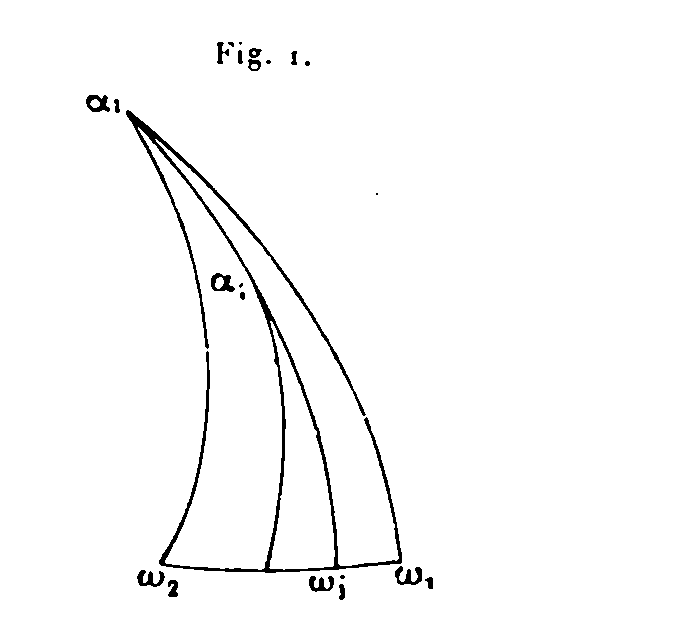
\includegraphics[width=0.43\textwidth]{fig1_scan.png}
\end{center}

Let
\begin{align*}
&\beta_1 \text{ be the point of the curve C whose abscissa is } x_0;\\
&\alpha_1 \text{ the corresponding point of the characteristic;}\\
&\alpha_1\omega_1 \text{ the tangent to the characteristic at } \alpha_1;\\
&\omega_1 \text{ the point where } \alpha_1\omega_1 \text{ meets the equator;}\\
&\alpha_i \text{ any point of the characteristic corresponding to a point } \beta_i \text{ situated to the right of } \beta_1;\\
&\alpha_i\omega_i \text{ the tangent at this point;}\\
&\omega_i \text{ the point where this tangent meets the equator.}
\end{align*}

When $\alpha_i$ advances on the characteristic, $\omega_i$ will move to the right, but will always remain on the arc of the equator $\omega_1\omega_2$\footnote{At present, $\omega_2$ designates one of the endpoints of a certain arc of the equator $\omega_1\omega_2$, which, by virtue of the third hypothesis, contains all the points $\omega_i$. (R. G.)}; the half-characteristic $\alpha_1\alpha_i$, which cannot cross the equator, is convex by hypothesis, and is entirely contained in the spherical triangle $\alpha_1\omega_1\omega_2$; that is, its curvilinear length always remains smaller than $\alpha_1\omega_1+\omega_1\omega_2$, that is, it is finite, which is absurd; the third hypothesis is therefore inadmissible.

\emph{Fourth hypothesis.} --- When $x$ varies from $x_0$ to infinity, the ordinate of the point $\beta_i$, that is, the direction angle of the tangent to the characteristic, always increases to infinity.

That is, the direction angle of the tangent to the characteristic can take all the values
\[
y_0+n\pi,
\]
where $y_0$ is a given constant and $n$ any positive integer. This is to say that the tangent of the direction angle, that is, the angular coefficient of the tangent to the characteristic, is equal to
\[
\operatorname{tang} y_0
\]
for an infinity of different points $\beta_i$.

Now the locus of the points where the angular coefficient of the tangent to the characteristic is equal to $\operatorname{tang} y_0$ is an algebraic curve which, by hypothesis, can meet the half-characteristic only in a finite number of points $\alpha_i$. It is therefore again necessary here that to a point $\alpha_i$ there correspond an infinity of points $\beta_i$, that is, that the given characteristic be a cycle.

In summary, of the four hypotheses that one may make, the first, the second and the fourth lead to this result, that the characteristic is a cycle; the third is inadmissible.

The theorem is therefore proved.

\emph{Definition.} --- We shall call a \emph{polycycle} a closed curve like the cycle, but presenting double points.

Example: the intersection of the sphere with a cylinder tangent to it at one point.

\emph{Topographic system.} --- If one draws on the sphere a system of cycles and polycycles such that through each of the points of the sphere there passes one cycle or polycycle, and only one, except at a few singular points through which no cycle passes, we shall say that this system of cycles is a \emph{topographic system}, because it is analogous to the system of level curves of a terrain.

The double points of the polycycles are then analogous to the saddles of this terrain; the singular points through which no cycle passes are analogous to the \emph{bottoms} and the \emph{summits} of the terrain; hence we shall call these various points the \emph{saddles, bottoms and summits} of the system.

For example, the system of curves
\[
f(x,y)=\operatorname{const.},
\]
where $f$ is an integral polynomial in $x$ and in $y$, is a topographic system if these curves do not cut the equator. The saddles are the points at which one has simultaneously
\[
\frac{df}{dx}=\frac{df}{dy}=0,
\qquad
\left(\frac{d^2f}{dx\,dy}\right)^2-\frac{d^2f}{dx^2}\frac{d^2f}{dy^2}>0;
\]
the summits are the points at which one has
\[
\frac{df}{dx}=\frac{df}{dy}=0,
\qquad
\left(\frac{d^2f}{dx\,dy}\right)^2-\frac{d^2f}{dx^2}\frac{d^2f}{dy^2}<0,
\qquad
\frac{d^2f}{dx^2}<0;
\]
the bottoms are the points at which one has
\[
\frac{df}{dx}=\frac{df}{dy}=0,
\qquad
\left(\frac{d^2f}{dx\,dy}\right)^2-\frac{d^2f}{dx^2}\frac{d^2f}{dy^2}<0,
\qquad
\frac{d^2f}{dx^2}>0.
\]

Similarly, if one has among $z$, $x$ and $y$ an algebraic relation
\[
f(z,x,y)=0,
\]
such that one never has
\[
\frac{df}{dz}=0,
\]
and such that $z$ cannot remain finite and real when $x$ and $y$ are infinite and real, the system of curves
\[
z=\operatorname{const.}
\]
is a topographic system.

For example, let
\[
f(z,x,y)=(z-x)^2-2(x^2+y^2+1)=0;
\]
\[
\frac{df}{dz}
\]
can vanish only if
\[
x^2+y^2+1=0,
\]
which is impossible.

Moreover, if one considers $z$ as a constant, the terms of the highest degree are written
\[
-(x^2+2y^2),
\]
that is, the curves $z=\operatorname{const.}$ do not cut the equator; in other words, these curves form a topographic system.

The locus of the points where each of the cycles of a topographic system is tangent to a characteristic will be called the \emph{curve of contacts}.

If the topographic system is algebraic, the curve of contacts will itself be an algebraic curve.

If one considers a topographic system and one of the polycycles of the system corresponding to one of the saddles of the system, part of the bottoms and summits lies outside the polycycle, another part inside, so that each saddle \emph{distributes in a certain manner} the bottoms and summits of the system.

Two topographic systems are \emph{analogous} when they have the same saddles, the same bottoms, the same summits, and when the bottoms and summits are \emph{distributed in the same manner by the saddles}.

\ornament

\setcounter{footnote}{0}

\begin{center}
{\bfseries CHAPTER II.}\\[0.8em]
{\scshape Study of the characteristics in the neighborhood of a point of the sphere.}
\end{center}

\shortline

Before studying the properties of the characteristics over the whole extent of the sphere, one must recall the results already obtained concerning the study of these curves in a limited region of the sphere. The principal theorems relating to this study are stated and proved in various memoirs of Cauchy, entitled \emph{Memoirs on the calculus of limits}, and inserted in volumes XIV, XV and XVI of the \emph{Comptes rendus des séances de l’Académie des Sciences}, and in the celebrated memoir of MM. Briot and Bouquet, inserted in volume XXXVI of the \emph{Journal de l’École Polytechnique}. I have myself dealt with this question in a Note found in the XLV\textsuperscript{e} fascicle of the \emph{Journal de l’École Polytechnique} and in a doctoral thesis that I defended before the Faculty of Sciences of Paris\footnote{See this Volume.}.

Let us first suppose that the point around which one wishes to study the characteristics is
\[
x=\alpha,\qquad y=\beta.
\]
X and Y, which are polynomials in $x$ and in $y$, may likewise be considered as polynomials in $x-\alpha$ and $y-\beta$.

Thus
\[
\begin{aligned}
X&=a_0+a_1(x-\alpha)+a_2(y-\beta)+\cdots,\\
Y&=b_0+b_1(x-\alpha)+b_2(y-\beta)+\cdots.
\end{aligned}
\]

\emph{First case.} --- $a_0$ and $b_0$ are not both zero; suppose, for example,
\[
a_0\gtrless0;
\]
the differential equation may be written
\[
\frac{dy}{dx}=\frac{Y}{X}=f(x,y),
\]
where $f$ is a series ordered according to increasing powers of $x-\alpha$ and $y-\beta$.

Therefore, by virtue of the theorem proved by Cauchy (\emph{Comptes rendus}, vol. XIV), $y$ may be expressed by a series ordered according to increasing powers of $x-\alpha$ and reducing to $\beta$ for $x=\alpha$.

Therefore through the point $(\alpha,\beta)$ passes one characteristic and only one.

\emph{Second case.} --- $a_0=b_0=0$.

But $a_1$, $a_2$, $b_1$ and $b_2$ are not all zero.

The point $(\alpha,\beta)$ is then an ordinary singular point. Let us begin by recalling a theorem concerning these singular points, a theorem which I proved in my inaugural thesis.

\emph{If the equation}
\[
\begin{array}{r@{\quad}c}
(5)&(a_1-\lambda)(b_2-\lambda)-b_1a_2=0
\end{array}
\]
\emph{has two different roots, $\lambda_1$ and $\lambda_2$;} 

\emph{If the ratio of these roots is positive or imaginary, the general integral of the equation}
\[
\frac{dx}{X}=\frac{dy}{Y}
\]
\emph{is of the form}
\[
z_1^{\lambda_1}z_2^{-\lambda_2}=\operatorname{const.},
\]
\emph{where $z_1$ and $z_2$ are series ordered according to increasing powers of $x-\alpha$, $y-\beta$ and vanishing for}
\[
x=\alpha,\qquad y=\beta.
\]

Suppose that the point $(x,y)$ approaches indefinitely the point $(\alpha,\beta)$, in such a way that
\[
\lim\frac{y-\beta}{x-\alpha}=\mu;
\]
the angular coefficient of the tangent at this point $(x,y)$ will have as its limit
\[
\frac{b_1+b_2\mu}{a_1+a_2\mu}.
\]

Therefore the limit of the line joining the points $(x,y)$ and $(\alpha,\beta)$ and the limit of the tangent to the characteristic at the point $(x,y)$ form a homographic pencil.

The double lines of this pencil are given by the equation
\[
\mu(a_1+a_2\mu)=b_1+b_2\mu.
\]

Let $\mu_1$ and $\mu_2$ be the two roots of this equation; one will easily calculate $\lambda_1$ and $\lambda_2$ as rational functions of $a_1$, $a_2$, $b_1$, $b_2$, $\mu_1$ and $\mu_2$.

Now one may divide the second case into four principal subordinate cases.

\emph{First subordinate case.} --- The double lines of the homographic pencil are real, and any two conjugate lines of the pencil are either both in the acute angle formed by the two double lines, or both in the obtuse angle.

In this case $\lambda_1$ and $\lambda_2$ are real and their ratio is positive; the theorem that we recalled at the beginning is therefore applicable, and the general integral is written
\[
z_1^{\lambda_1}z_2^{-\lambda_2}=\operatorname{const.},
\]
where $z_1$, $z_2$ are real functions of $x$ and of $y$ vanishing for
\[
x=\alpha,\qquad y=\beta,
\]
while $\lambda_1$ and $\lambda_2$ are two positive real numbers.

It follows that all the characteristics will pass through the singular point $(\alpha,\beta)$, provided that they enter a region of the sphere sufficiently near this point for $z_1$ and $z_2$ to be convergent.

Such a singular point will be called a \emph{node}.

Let us, for example, study the characteristics which satisfy the equation
\[
\frac{dx}{x}=\frac{dy}{2y}
\]
in the neighborhood of the point
\[
x=y=0.
\]

The general equation of these characteristics will be written
\[
y=kx^2,
\]
where $k$ is a constant. In the plane this equation represents a series of parabolas having the same axis and having their vertex at the origin; on the sphere this same equation will represent the intersections of the sphere with the cones that have the center of the sphere for vertex and these parabolas for base.

All these intersections evidently pass through the point
\[
x=y=0.
\]

\emph{Second subordinate case.} --- The double lines of the homographic pencil are real; but two conjugate lines of the pencil are situated on opposite sides of these two double lines.

In this case $\dfrac{\lambda_1}{\lambda_2}$ is real and negative, and the theorem of which we have spoken is no longer applicable.

But MM. Briot and Bouquet showed, in a memoir inserted in the \emph{Journal de l’École Polytechnique}, XXXVI\textsuperscript{e} fascicle, that through the point $(\alpha,\beta)$ pass two characteristics and two only.

Such a singular point will be called a \emph{saddle}.

Let us, for example, study in the neighborhood of the origin the characteristics defined by the equation
\[
\frac{dx}{x}=-\frac{dy}{y}.
\]

The general integral is written
\[
xy=\operatorname{const.}
\]
and the only characteristics which pass through the point
\[
x=y=0
\]
are the two great circles
\[
x=0,\qquad y=0.
\]

\emph{Third subordinate case.} --- The double lines of the homographic pencil are imaginary, and this pencil does not reduce to a system of lines in involution.

In this case $\lambda_1$ and $\lambda_2$ are two conjugate imaginaries and their ratio is imaginary. The general theorem applies and the general integral is written
\[
z_1^{\lambda_1}z_2^{-\lambda_2}=\operatorname{const.},
\]
where $z_1$ and $z_2$, $\lambda_1$ and $\lambda_2$ are conjugate imaginaries.

Let
\[
\begin{aligned}
z_1&=\xi+i\eta,& \lambda_1&=\gamma+i\delta,\\
z_2&=\xi-i\eta,& \lambda_2&=-\gamma+i\delta.
\end{aligned}
\]

The general integral is then written
\[
(\xi^2+\eta^2)^\gamma\left(\frac{\xi+\eta i}{\xi-\eta i}\right)^{i\delta}=\operatorname{const.}
\]

The curves $\xi^2+\eta^2=\operatorname{const.}$ (where $\xi$ and $\eta$ are series ordered according to increasing powers of $x-\alpha$ and $y-\beta$, and vanishing for $x=\alpha$, $y=\beta$) are evidently cycles which do not cut one another at any point and which form, in the region neighboring the point $(\alpha,\beta)$, a topographic system of which the point $(\alpha,\beta)$ is a summit.

Now, if one observes that the equations
\[
\xi^2+\eta^2=A,
\qquad
\left(\frac{\xi+i\eta}{\xi-i\eta}\right)^i=B
\]
give for $\xi$ and $\eta$, and consequently for $x$ and $y$, only a single system of real values, one will recognize that the characteristics cut the cycles
\[
\xi^2+\eta^2=A
\]
at only a single point and that, consequently, these characteristics are nothing other than spirals; a point which traverses these spirals in a certain direction approaches the origin indefinitely.

Such a singular point will be called a \emph{focus}.

Let, for example, the equation be
\[
\frac{dx}{x-y}=\frac{dy}{x+y},
\]
whose general integral is
\[
(x^2+y^2)\left(\frac{x+iy}{x-iy}\right)^i=\operatorname{const.}
\]

If one passes to polar coordinates, this integral becomes
\[
\rho^2e^{-2\omega}=\operatorname{const.},
\]
which gives us, in the plane, a logarithmic spiral and, consequently, on the sphere, a spherical spiral.

\emph{Fourth subordinate case.} --- The double lines of the homographic pencil are imaginary and this pencil reduces to a system of lines in involution.

In this case $\lambda_1$ and $\lambda_2$ are conjugate imaginaries, but their ratio is equal to $-1$. The theorem that we recalled at the beginning is therefore not applicable in general.

This fourth case is more particular than the preceding ones and will not occur if X and Y are the most general polynomials of their degree. Let us therefore confine ourselves to a few remarks.

First, it is impossible for a branch of a characteristic to come to pass through the point $\alpha$, $\beta$, since its tangent would have to be precisely one of the double lines of the involution, which are imaginary.

But, from what will be seen below, every characteristic is a cycle or a spiral; therefore either the characteristics will be spirals, and a point which traversed them would turn around the point $(\alpha,\beta)$ while approaching it indefinitely: the point $(\alpha,\beta)$ would then again be a \emph{focus}; or else the characteristics form a topographic system of which $(\alpha,\beta)$ is a summit, and then the point $(\alpha,\beta)$ is a \emph{center}.

This is what occurs when the theorem that we stated at the beginning is applicable, despite the negative value of $\dfrac{\lambda_1}{\lambda_2}$.

Indeed, in this case, the integral is written
\[
z_1z_2=A,
\]
where
\[
z_1=\xi+i\eta,
\qquad
z_2=\xi-i\eta;
\]
that is,
\[
\xi^2+\eta^2=A;
\]
and the characteristics evidently form, in this case, a topographic system of cycles.

For example, the equation
\[
\frac{dx}{y}=\frac{dy}{-x}
\]
has for general integral
\[
x^2+y^2=A.
\]

\emph{Particular cases left aside.} --- In what precedes, one has left aside the particular cases where
\[
\lambda_1=\lambda_2,
\qquad
\lambda_1=0,
\]
cases which will not occur if X and Y are the most general polynomials of their degree.

Now, in order that
\[
\lambda_1=\lambda_2,
\]
it is necessary and sufficient that
\[
(a_1+b_2)^2-b_1a_2+a_1b_2=0.
\]

In this case, MM. Briot and Bouquet showed that an infinity of characteristics pass through the point $(\alpha,\beta)$, that is, that one is again dealing with a \emph{node}.

The five preceding cases include all the singular points $\alpha$, $\beta$, such that the two curves
\[
X=0,\qquad Y=0
\]
cut one another there in a single point and not in several coincident points. These singular points will be called \emph{singular points of the first kind}, and it has been seen that there are four sorts of such points: nodes, saddles, foci, and centers.

It remains to examine the cases where
\[
\lambda_1=0
\]
and those where
\[
a_1=a_2=0
\]
or
\[
b_1=b_2=0.
\]

These cases occur when the curves $X=Y=0$ cut one another in several points coincident at the point $(\alpha,\beta)$.

Indeed, to say that
\[
a_1=a_2=0,
\]
is to say that $X=0$ presents a multiple point at $(\alpha,\beta)$.

To say that
\[
b_1=b_2=0,
\]
is to say that $Y=0$ presents a multiple point at $(\alpha,\beta)$.

To say that
\[
\lambda_1=0,
\]
is to say that
\[
\frac{a_1}{a_2}=\frac{b_1}{b_2},
\]
that is, that the curves $X=0$, $Y=0$ are tangent at the point $(\alpha,\beta)$.

Such singular points will be called \emph{singular points of the second kind}, and it is evident, from what precedes, that they may always be considered as the limit of a system of several singular points of the first kind coincident together.

The particularities which such points may present are too numerous and too diverse for us to study them in detail. Let us remark that such points cannot exist if X and Y are the most general polynomials of their degree.

\emph{Points situated on the equator.} --- In what precedes, one has implicitly supposed that $\alpha$ and $\beta$ remain finite, that is, that the point $(\alpha,\beta)$ is not on the equator.

But the case in which $\alpha$, $\beta$ is on the equator may easily be reduced to the cases already studied.

First consider a point of the equator not situated on the great circle
\[
x=0;
\]
we shall set
\[
x=\frac1z,
\qquad
y=\frac{t}{z}.
\]

If one then considers $z$ and $t$ as the coordinates of a point in a plane, this point will be nothing other than the gnomonic projection of the point $(x,y)$ of the sphere onto a plane parallel to the plane of the great circle
\[
x=0.
\]

For the point $(\alpha,\beta)$ of the sphere, these coordinates $z$ and $t$ will be finite, that is, one will be brought back to the cases studied at the beginning of this Chapter.

If one wished to study the characteristics in the neighborhood of the intersection of the equator and the great circle
\[
x=0,
\]
one would set
\[
x=\frac{t}{z},
\qquad
 y=\frac1z,
\]
and one would reason in the same way.

\ornament


\ornament
\begin{center}
{\Large CHAPTER III.}\\[0.4em]
{\small DISTRIBUTION OF SINGULAR POINTS.}
\end{center}
\shortline

\emph{Theorem II.} --- \emph{Every system of characteristics admits singular points.}

\emph{First hypothesis.} --- The curves
\[
X=0,\qquad Y=0
\]
meet in points not situated on the equator.

In this case, these points of intersection are evidently singular points.

\emph{Second hypothesis.} --- The curves
\[
X=0,\qquad Y=0
\]
meet in a point situated on the equator.

Suppose that this point is not on the great circle
\[
x=0;
\]
we shall put
\[
x=\frac1z,\qquad y=\frac{t}{z},
\]
and, if $m$ is the degree of that one of the two polynomials X and Y whose degree is the greater, we shall put
\[
z^mX=X_1,\qquad z^mY=Y_1.
\]
The differential equation then becomes
\[
\frac{dz}{zX_1}=\frac{dt}{Y_1-tX_1};
\]
for $t=\alpha$, $z=0$, one has, by hypothesis,
\[
Y_1=X_1=0,
\]
and consequently
\[
zX_1=0,\qquad Y_1-tX_1=0,
\]
that is, the point
\[
t=\alpha,\qquad z=0
\]
is a singular point of the proposed equation.

\emph{Third hypothesis.} --- The curves $X=0$, $Y=0$ meet in no point. The degree of X is greater than that of Y. In this case, at least one of the two polynomials X and Y is of even degree. Moreover $Y_1$ is divisible by $z$, so that
\[
Y_1=zY_2.
\]
Now it is clear that for
\[
z=t=0,
\]
one has
\[
zX_1=zY_2-tX_1=0,
\]
and consequently the point
\[
z=t=0
\]
is a singular point.

\emph{Fourth hypothesis.} --- The curves $X=0$, $Y=0$ meet in no point. The degree of X is less than that of Y. In this case one would put
\[
x=\frac{t}{z},\qquad y=\frac1z,
\]
and, reasoning as in the preceding case, one would see that
\[
z=t=0
\]
is a singular point.

\emph{Fifth hypothesis.} --- The curves $X=0$, $Y=0$ meet in no point. The degree of X and that of Y is the same.

If, moreover, $X_2$ and $Y_2$ are the terms of highest degree of X and Y, one does not have identically
\[
xY_2-yX_2=0.
\]
In this case, the degree of X and Y being $m$, and necessarily even, the function $xY_2-yX_2$ is homogeneous in $x$ and $y$ and of degree $m+1$, and consequently of odd degree.

It therefore vanishes either for $x=0$ or for a certain finite value of $\dfrac yx$.

If it vanishes for a certain value $\alpha$ of $\dfrac yx$, one will have at the same time, for
\[
t=\alpha,\qquad z=0,
\]
\[
zX_1=Y_1-tX_1=0
\]
when one has put
\[
x=\frac1z,\qquad y=\frac{t}{z},
\]
that is, the point
\[
t=\alpha,\qquad z=0
\]
will be a singular point.

If the function $xY_2-yX_2$ vanishes for $x=0$, one will put
\[
x=\frac{t}{z},\qquad y=\frac1z,
\]
and one will see, as before, that the point
\[
t=z=0
\]
is a singular point.

\emph{Sixth hypothesis.} --- The curves X and Y meet in no point. The degree of X is the same as that of Y; if, moreover, $X_2$ and $Y_2$ are the terms of highest degree of X and Y, one has identically
\[
xY_2-yX_2=0.
\]
This hypothesis is inadmissible.

Indeed, if one has identically
\[
xY_2=yX_2,
\]
$X_2$ is divisible by $x$ and equal to $xX_3$, $Y_2$ is divisible by $y$ and equal to $yY_3$, so that one has identically
\[
xyY_3=yxX_3
\]
or
\[
Y_3=X_3.
\]
Now $Y_3=X_3$ is a homogeneous function of odd degree in $x$ and in $y$; hence it vanishes either for $x=0$ or for a certain real value $\alpha$ of $\dfrac yx$.

Therefore, either for $x=0$ or for $\dfrac yx=\alpha$, one would necessarily have
\[
X_2=Y_2=0,
\]
that is, the curves $X=0$, $Y=0$ would meet at a point of the equator, which is contrary to the hypothesis.

In summary, of the six hypotheses that one can make, the sixth is inadmissible; if one of the other five is realized, the differential equation admits singular points, either on the equator or outside the equator.

\emph{General case.} --- One may, without loss of generality, suppose:

1° That the polynomials X and Y are of the same degree;

2° That if $X_2$ and $Y_2$ are the terms of highest degree of X and Y, one does not have identically
\[
xY_2-yX_2=0;
\]
3° That the curves $X=Y=0$ nowhere meet in several coincident points and do not meet on the equator;

4° That the equation
\[
xY_2-yX_2=0
\]
has no multiple roots.

In this case, \emph{the equator is always a characteristic}, and all singular points are of the first species. Moreover, without loss of generality, one may suppose that all the singular points are \emph{nodes}, \emph{saddles} and \emph{foci}.

\emph{The number of singular points is evidently even}, since everything is symmetric with respect to the center of the sphere.

The minimum number of singular points is therefore equal to $2$, and this case can occur in two ways:

1° The curves
\[
X=0,\qquad Y=0
\]
do not meet at any point; but the homogeneous equation
\[
xY_2-yX_2=0
\]
admits one and only one real solution.

There are then on the equator two diametrically opposite singular points. I say that these singular points are always nodes. To prove this, it is necessary to study the general properties of singular points situated on the equator.

Suppose that for
\[
t=\alpha,\qquad z=0,
\]
one has
\[
zX_1=Y_1-tX_1=0
\]
and
\[
X_1\gtrless0,\qquad Y_1\gtrless0.
\]
Put
\[
t=u+\alpha,
\]
and let
\[
\begin{aligned}
X_1&=z\xi_1+\lambda_0+\lambda_1u+\lambda_2u^2+\cdots+\lambda_mu^m,\\
Y_1&=z\eta_1+\mu_0+\mu_1u+\mu_2u^2+\cdots+\mu_mu^m,
\end{aligned}
\]
where $\xi_1$ and $\eta_1$ are integral polynomials in $z$ and in $u$, and where the $\lambda$'s and the $\mu$'s are constants. It follows, putting
\[
\begin{aligned}
\lambda_2u^2+\cdots+\lambda_mu^m&=\xi_2u^2,\\
\mu_2u^2+\cdots+\mu_mu^m&=\eta_2u^2,\\
X_1&=u^2\xi_2+z\xi_1+\lambda_0+\lambda_1u,\\
Y_1&=u^2\eta_2+z\eta_1+\mu_0+\mu_1u;
\end{aligned}
\]
whence one obtains
\[
Y_1-tX_1=z\theta_1+u^2\theta_2+(\mu_0-\lambda_0\alpha)+(\mu_1-\lambda_1\alpha-\lambda_0)u,
\]
where $\theta_1$ and $\theta_2$ are integral polynomials in $z$ and $u$. The differential equation is then written, noting that one must have $\mu_0=\lambda_0\alpha$,
\[
\frac{dz}{z(\lambda_0+\lambda_1u+z\xi_1+u^2\xi_2)}=
\frac{du}{(\mu_1-\lambda_1\alpha-\lambda_0)u+z\theta_1+u^2\theta_2}.\tag{1}
\]
The roots of equation (5) are then
\[
-\lambda_0\quad\text{and}\quad \mu_1-\lambda_1\alpha-\lambda_0.
\]
These two roots are real.

Thus \emph{every singular point situated on the equator is a node or a saddle}. (This is what one should have foreseen, since the equator is a characteristic.)

For it to be a node, it is necessary and sufficient that
\[
\lambda_0^2+\lambda_0\lambda_1\alpha-\lambda_0\mu_1>0.
\]
Now the first member of this inequality is precisely the value taken, for
\[
y=x\alpha,
\]
by the expression
\[
-\frac1{x^{2m}}\frac{d}{dy}(xY_2X_2-yX_2^2).
\]
We shall not change its sign by writing\footnote{In this sentence, an editorial error has been corrected. (R. G.).}
\[
-\frac{d}{dy}\left(\frac{Y_2}{X_2}-\frac yx\right),
\]
that is, the singular point
\[
\frac yx=\alpha
\]
will be a saddle if, when $\dfrac yx$ passes from $\alpha-\varepsilon$ to $\alpha+\varepsilon$, the expression $\dfrac{Y_2}{X_2}-\dfrac yx$ passes from negative to positive, and it will be a node if, when $\dfrac yx$ passes from $\alpha-\varepsilon$ to $\alpha+\varepsilon$, the expression $\dfrac{Y_2}{X_2}-\dfrac yx$ passes from positive to negative.

With this done, we shall introduce a new consideration which will be of the greatest service to us. Let a cycle be situated entirely in one hemisphere. This cycle divides the sphere into two regions, one of which, situated entirely in one of the hemispheres, will be called \emph{the interior of the cycle}.

If the cycle is entirely in the first hemisphere, we shall say that a moving point describes the cycle in the positive sense if it constantly has the interior of the cycle \emph{on its left}; if, on the contrary, the cycle were in the second hemisphere, a point would describe the cycle in the positive sense if it constantly had the interior \emph{on its right}.

Suppose that a moving point describes the cycle in the positive sense and consider the variations of the expression $\dfrac YX$. Let $h$ be the number of times this expression jumps from $-\infty$ to $+\infty$; let $k$ be the number of times this expression jumps from $+\infty$ to $-\infty$. Let
\[
i=\frac{h-k}{2};
\]
the number $i$ will be called \emph{the index of the cycle}.

If one joins two points A and C of a cycle ABCDA by an arc AMC situated
\begin{center}
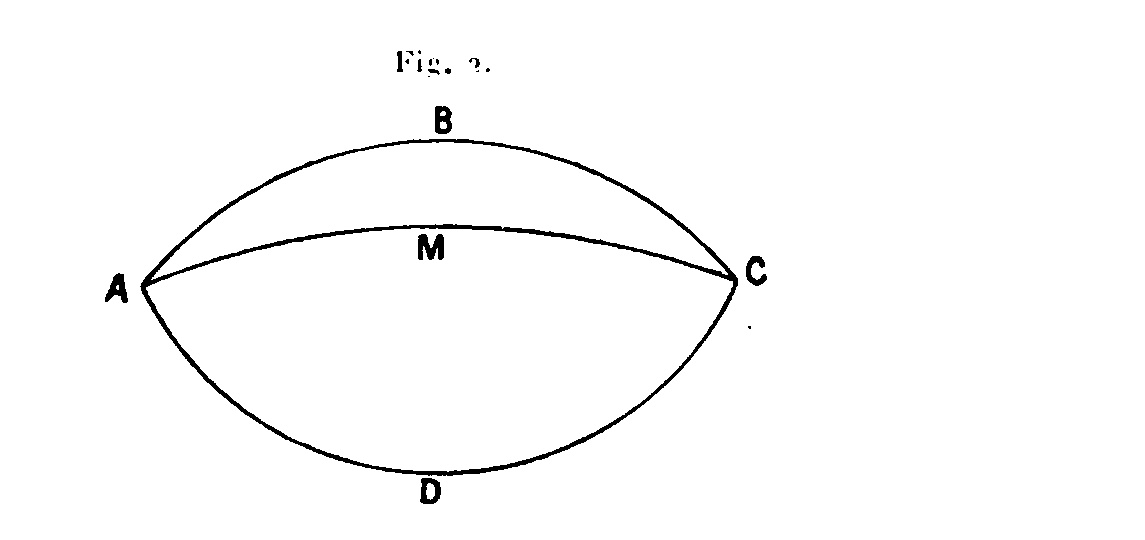
\includegraphics[width=0.48\textwidth]{fig2_scan.jpg}
\end{center}
entirely in the interior of the cycle, the cycle ABCDA is decomposed into two cycles ABCMA, AMCDA, and one evidently has
\[
\operatorname{ind.}ABCDA=\operatorname{ind.}ABCMA+\operatorname{ind.}AMCDA,
\]
so that one can reduce the calculation of the index of any cycle to the calculation of the index of the different infinitely small cycles which compose it.

\emph{Theorem III.} --- \emph{An infinitely small cycle which contains in its interior no singular point has index $0$.}

Indeed, if this cycle is not cut by the curve $X=0$,
\[
h=0,\qquad k=0,\qquad i=\frac{h-k}{2}=0.
\]
If the cycle is cut by the curve $X=0$, it is not cut by the curve $Y=0$; Y is always of the same sign and X passes once from positive to negative, once from negative to positive; whence
\[
h=1,\qquad k=1,\qquad i=\frac{h-k}{2}=0.
\]
Similarly, if the curve $X=0$ presented in the interior of the cycle a multiple point of order $m$, one would have
\[
h=m,\qquad k=m,\qquad i=\frac{h-k}{2}=0.
\]

\emph{Theorem IV.} --- \emph{If an infinitely small cycle contains in its interior a singular point, its index is equal to $\pm1$.}

It is equal to $+1$ if the singular point is a saddle; to $-1$ if the singular point is a node or a focus.

Indeed, put
\[
y-\beta=\rho\sin\omega,\qquad x-\alpha=\rho\cos\omega,
\]
and suppose that one considers the cycle
\[
(y-\beta)^2+(x-\alpha)^2=\rho^2,
\]
$\rho$ being an infinitely small constant.

To describe this cycle in the positive sense, one must make $\omega$ vary from $0$ to $2\pi$.

Now, neglecting infinitesimals and taking again the notations of the preceding chapter, one has
\[
\frac YX=\frac{b_1+b_2\operatorname{tang}\omega}{a_1+a_2\operatorname{tang}\omega}.
\]
X vanishes twice, for, when $\omega$ varies from $0$ to $2\pi$,
\[
a_1+a_2\operatorname{tang}\omega
\]
vanishes twice for two values of $\omega$ which we shall call $\omega_0$ and $\omega_0+\pi$.

For $\omega=\omega_0-\varepsilon$, where $\varepsilon$ is infinitely small, one has
\[
\operatorname{tang}\omega=\operatorname{tang}\omega_0-\zeta,
\]
where $\zeta$ is positive and infinitely small. Thus
\[
\frac YX=\frac{b_1+b_2\operatorname{tang}\omega_0-b_2\zeta}{a_1+a_2\operatorname{tang}\omega_0-a_2\zeta}.
\]
Observe that $\operatorname{tang}\omega_0=-\dfrac{a_1}{a_2}$; it will come, neglecting $b_2\zeta$ before $b_1+b_2\operatorname{tang}\omega_0$,
\[
\frac YX=\frac{a_1b_2-a_2b_1}{a_2^2}\,\frac1\zeta.
\]
Therefore, if $a_1b_2-a_2b_1<0$, $\dfrac YX$ for $\omega=\omega_0$ and for $\omega=\omega_0+
\pi$ jumps from $-\infty$ to $+\infty$, and one has
\[
h=2,\qquad k=0,\qquad i=\frac{h-k}{2}=1.
\]
If, on the contrary, $a_1b_2-a_2b_1>0$, $\dfrac YX$ for $\omega=\omega_0$ and for $\omega=\omega_0+
\pi$ jumps from $+\infty$ to $-\infty$, and one has
\[
h=0,\qquad k=2,\qquad i=\frac{h-k}{2}=-1.
\]
Now, what is the condition for
\[
a_1b_2-a_2b_1>0?
\]
Let us take again equation (5), which is written
\[
(a_1-\lambda)(b_2-\lambda)-a_2b_1=0.
\]
It is evident that one will have
\[
a_1b_2-a_2b_1>0,
\]
if the two roots of the equation are imaginary or of the same sign, that is, if the singular point is a node or a focus. On the contrary one will have
\[
a_1b_2-a_2b_1<0,
\]
if the two roots are real and of opposite signs, that is, if the singular point is a saddle.

The theorem is therefore proved.

\emph{Problem I.} --- \emph{Calculate the index of a cycle situated entirely in one of the hemispheres.}

Let N be the number of nodes, F the number of foci, C the number of saddles contained in the interior of the cycle.

If one decomposes the given cycle into an infinity of infinitely small cycles $\gamma$,
\[
\begin{array}{rcl}
\text{An infinite number of cycles }\gamma\text{ will have index} & 0,\\
N+F\text{ cycles }\gamma & -1,\\
C\text{ cycles }\gamma & +1.
\end{array}
\]
The index of the given cycle will therefore be
\[
-(N+F-C).
\]

\emph{Problem II.} --- \emph{Calculate the index of the equator.}

Let $2N'$ be the number of nodes, $2C'$ the number of saddles situated on the equator.

Let $t=\dfrac yx=\operatorname{tang}\omega$.

Make $\omega$ vary from $-\dfrac\pi2$ to $+\dfrac\pi2$, that is, $\operatorname{tang}\omega$ from $-\infty$ to $+\infty$. Since everything is symmetric with respect to the center of the sphere,
\[
\frac YX=\frac{Y_2}{X_2}
\]
takes for $\omega+\pi$ the same value as for $\omega$; if one made $\omega$ vary from $+\dfrac\pi2$ to $+\dfrac{3\pi}{2}$, $\dfrac YX$ would pass again through the same values as when $\omega$ varied from $-\dfrac\pi2$ to $+\dfrac\pi2$.

Therefore, as $\omega$ varies from $-\dfrac\pi2$ to $+\dfrac\pi2$, $\dfrac YX$ will jump $\dfrac h2$ times from $-\infty$ to $+\infty$, and $\dfrac k2$ times from $+\infty$ to $-\infty$.

This being so, if one considers the expression
\[
H=\frac{Y_2}{X_2}-\frac yx=\frac YX-\operatorname{tang}\omega,
\]
for $\omega=-\dfrac\pi2$, one has
\[
H=+\infty;
\]
for $\omega=+\dfrac\pi2$, one has
\[
H=-\infty.
\]
Let $\lambda$ be the number of times that H passes from negative to positive, $\mu$ the number of times that H passes from positive to negative; one will evidently have
\[
\mu-\lambda=1.
\]
Now H can pass from negative to positive either through 0, which corresponds to a saddle, or through $\infty$, which corresponds to one of the values among the $\dfrac h2$ values of $\omega$ for which $\dfrac YX$ jumps from $-\infty$ to $+\infty$.

One therefore has
\[
\lambda=C'+\frac h2.
\]
Similarly
\[
\mu=N'+\frac k2;
\]
whence
\[
N'-C'=1+\frac{h-k}{2}=1+i,
\]
whence
\[
i=N'-C'-1.
\]

\emph{Scholium.} --- If the number of nodes situated outside the equator is $2N$, that of the foci situated outside the equator $2F$, that of the saddles situated outside the equator $2C$, that of the nodes situated on the equator $2N'$, that of the saddles situated on the equator $2C'$, one has the relation
\[
N'+N+F=C+C'+1.
\]
Indeed, to obtain this result it suffices to equate the two values of the index of the equator obtained in the two preceding problems.

\emph{Corollary I.} --- The total number of nodes and foci is equal to the total number of saddles plus $2$.

\emph{Corollary II.} --- The total number of singular points is a multiple of $4$ plus $2$.

\emph{Corollary III.} --- If the number of singular points is reduced to $2$, these points are nodes and foci; they are always nodes if they are on the equator.

The curve $X=0$ and the curve $Y=0$ are composed of a certain number of cycles. Consider any two of these cycles: they will meet in an even number of points.

Let $\alpha_0$, $\alpha_1$, \ldots, $\alpha_{2n}$ be the $2n$ points of intersection of these two cycles arranged according to the order in which one meets them when traversing one of the two cycles, the cycle $X=0$, for example, in the positive sense.

\emph{Theorem V.} --- \emph{Suppose that two consecutive points $\alpha_k$ and $\alpha_{k+1}$ are situated in the same hemisphere: I say that if $\alpha_k$ is a node or a focus, $\alpha_{k+1}$ is a saddle, or reciprocally.}

For this it suffices to show that every cycle which envelops $\alpha_k$ and $\alpha_{k+1}$ has index $0$.

Indeed, let (fig. 3) AB be the arc of the cycle $X=0$ on which the points $\alpha_k$ and $\alpha_{k+1}$ lie; let CD and EF be the arcs of the cycle $Y=0$ which cut AB respectively at $\alpha_k$ and $\alpha_{k+1}$.
\begin{center}
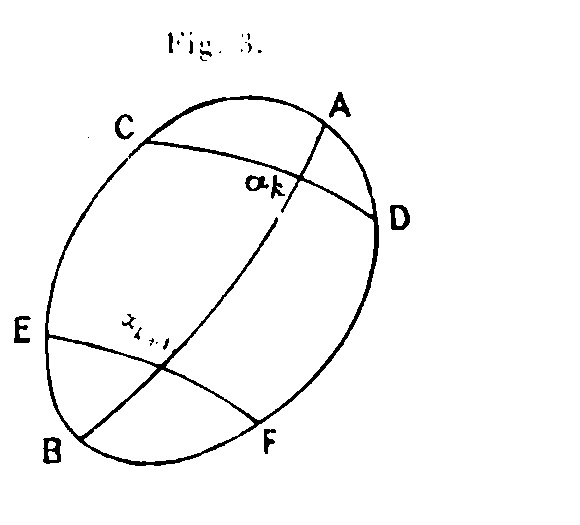
\includegraphics[width=0.30\textwidth]{fig3_scan.jpg}
\end{center}
It is evident that, for the cycle ADFBECA,
\[
h=1,\qquad k=1,\qquad i=\frac{h-k}{2}=0.
\]
Suppose, on the contrary, that the points $\alpha_k$ and $\alpha_{k+1}$ are in two different hemispheres:
\begin{center}
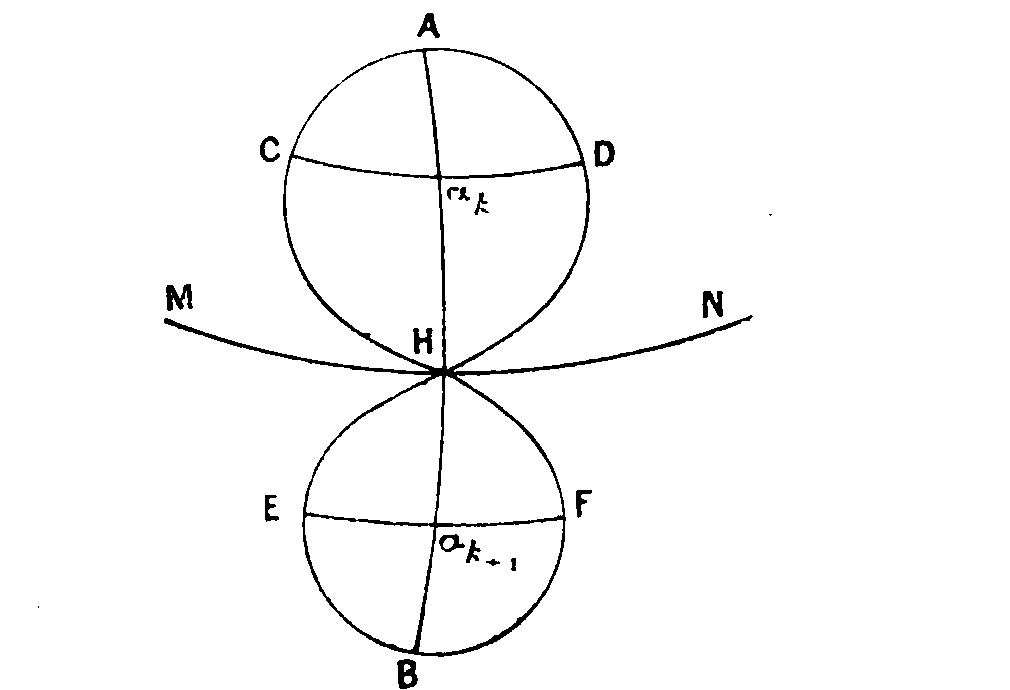
\includegraphics[width=0.38\textwidth]{fig4_scan.jpg}
\end{center}
I say that if $\alpha_k$ is a saddle, $\alpha_{k+1}$ is a saddle, and that if $\alpha_k$ is a node or a focus, $\alpha_{k+1}$ is a node or a focus.

Indeed, suppose that AB cuts the equator MN at H (fig. 4). Consider the cycle ACHFBEHDA. This cycle is traversed \emph{in the two hemispheres} in the positive sense.

Suppose that, in crossing the point A, $\dfrac YX$ jumps from $-\infty$ to $+\infty$; the same will occur when one crosses the point H or the point B, that is to say, if
\[
\operatorname{ind.}ACHD=1,\qquad \operatorname{ind.}ACHFBEHDA=2.
\]
Similarly, if
\[
\operatorname{ind.}ACHD=-1,\qquad \operatorname{ind.}ACHFBEHDA=-2,
\]
that is, in all cases,
\[
\operatorname{ind.}ACHDA=\operatorname{ind.}HFBEH.
\]
Q. E. D.

\emph{Second case.} --- In all that precedes, we have supposed that $X_2$ and $Y_2$ were of the same degree, without
\[
xY_2-yX_2
\]
being identically zero.

We have not examined what would happen if we had identically
\[
xY_2-yX_2=0.
\]
From a certain point of view, the case which we have studied is more general than the one which we left aside.

From another point of view, it is the contrary; for any two polynomials X and Y may be considered as special cases of the polynomials
\[
X+\lambda xZ,
\qquad
Y+\lambda yZ,
\]
where $\lambda$ is a constant and Z a polynomial of the same degree as X and Y.

We shall therefore suppose that one has identically
\[
X_2=xZ,
\qquad
Y_2=yZ,
\]
where Z is a homogeneous function in $x$ and $y$.

In this case, \emph{the equator is no longer a characteristic}, and consequently the singular points of the equator may just as well be nodes, foci, or saddles.

The rule which made it possible, in the preceding case, to find the index of the equator fails; moreover, if the equator contains singular points, the curves
\[
X=0,
\qquad
Y=0
\]
meet on this great circle, which consequently no longer has, properly speaking, an index.

Suppose therefore that the equator contains no singular point, and let us seek the index of this great circle.

We shall find that along the equator one has
\[
\frac YX=\frac yx,
\]
that is, the index of the equator will be equal to $-1$, and if one observes that it is already equal to
\[
-(N+F-C),
\]
$2N$, $2F$, $2C$ being the number of nodes, foci, and saddles, one will recognize that
\[
F+N=C+1,
\]
that is, the theorem which had been proved in the preceding case is still true.

Suppose now that the equation contains singular points, namely $2N'$ nodes, $2F'$ foci, and $2C'$ saddles, and let us see how one can get around the difficulty.

Let $\alpha x+\beta y+\gamma=0$ be a great circle passing through no singular point.

Put
\[
x'=\frac{x}{\alpha x+\beta y+\gamma},
\qquad
 y'=\frac{y}{\alpha x+\beta y+\gamma};
\]
the differential equation becomes
\[
\frac{dx'}{X'}=\frac{dy'}{Y'},
\]
where $X'$ and $Y'$ are integral polynomials in $x'$ and $y'$.

One can have chosen the circle $\alpha x+\beta y+\gamma=0$ in such a way that:

1° No reduction taking place, $X'$ and $Y'$ are of the same degree;

2° The great circle $\alpha x+\beta y+\gamma=0$ is not a characteristic, that is, the terms of highest degree of $y'X'-x'Y'$ reduce.

If $a$, $b$ is a singular point of the equation
\[
\frac{dx}{X}=\frac{dy}{Y},
\]
\[
a'=\frac{a}{\alpha a+\beta b+\gamma},
\qquad
b'=\frac{b}{\alpha a+\beta b+\gamma},
\]
will also be a singular point of the equation
\[
\frac{dx'}{X'}=\frac{dy'}{Y'}.
\]
If $a$, $b$ is a node, a saddle or a focus, $a'$, $b'$ will be a node, a saddle or a focus, so that the numbers of nodes, saddles and foci are $2(N+N')$, $2(C+C')$, $2(F+F')$, and, being reduced to the case where the equator contained no singular point, one can write
\[
N+N'+F+F'=C+C'+1.
\]

\ornament



\ornament
\begin{center}
{\Large CHAPTER IV.}\\[0.4em]
{\small THEORY OF CONTACTS.}
\end{center}
\shortline

The study that we have just made of the singular points will finally allow us to approach the question of the geometrical forms which the characteristics can assume \emph{over the whole surface of the sphere}.

A first consideration, of capital importance, is that of the number of points at which a given arc or cycle touches a characteristic, that is, the number of contacts of this arc or of this cycle.

The number of contacts of an algebraic arc or of an algebraic cycle is always finite.

\emph{Preliminary remarks.} --- We have seen that an algebraic curve without a double point is composed of a certain number of cycles; likewise an algebraic curve with double points is composed of a certain number of cycles and polycycles. Now these polycycles themselves can be regarded as decomposable into a certain number of cycles touching at the double points and presenting angular points at these points.

Thus the curve
\[
x^2-y^2=(x^2+y^2)^2
\]
is composed of two diametrically opposite polycycles; each of these polycycles is composed of two cycles which touch at the point
\[
x=y=0
\]
and there present an angular point such that the axis of the two tangents is $90^\circ$.

We have seen that an algebraic curve C cuts any algebraic cycle in a finite and even number of points. This calls for a few explanations.

If, at a given point, the algebraic curve C passes from the interior of the cycle to the exterior, or conversely, we shall say that the curve \emph{crosses} the cycle, and this point will count as a single point of intersection or as an odd number of coincident points of intersection. If, on the contrary, in the neighborhood of a given point common to the curve C and to the cycle, the curve C remains entirely outside or inside the cycle, we shall say that the curve \emph{touches} the cycle, and this point will count as an even number of coincident points of intersection.

Suppose, for example, that the given cycle has an angular point at the origin and that its equation is written
\[
0=(y-\lambda x)(y-\mu x)+\theta_3,
\]
where $\theta_3$ is a polynomial containing only terms of degree $3$ and higher.

Suppose that a point infinitely near the origin is inside the given cycle whenever\footnote{Here, as below, pp. 35 and 36, various changes of signs have been introduced in the editing. (R. G.)}
\[
x>0,\qquad (y-\lambda x)(y-\mu x)<0,
\]
and outside if
\[
x<0\qquad\text{or if}\qquad x>0,\qquad (y-\lambda x)(y-\mu x)>0.
\]
Let
\[
0=y-mx+\theta_2
\]
be the equation of the curve C, where $\theta_2$ denotes a polynomial containing only terms of degree $2$ and higher.

It is easy to see that the curve C crosses the cycle whenever
\[
(m-\lambda)(m-\mu)<0
\]
and touches it in the contrary case.

\emph{Theorem VI.} --- \emph{The number of contacts of an algebraic cycle which has no angular point, has no contact of higher order with a characteristic, and passes through no singular point is always finite and even.}

Indeed, let
\[
\mathrm F(x,y)=0
\]
be the equation of this cycle. Its contacts will be found by seeking its intersection with the curve
\[
\varphi=X\frac{d\mathrm F}{dx}+Y\frac{d\mathrm F}{dy}=0.
\]
Since this curve is algebraic, its intersections with the given cycle are even in number, provided one takes care to count twice those points at which the curve touches the cycle. But at these points the cycle would have, with a characteristic, a contact of even order, which we have not assumed. Hence nowhere are there several coincident points of intersection of the curves
\[
\varphi=0,\qquad \mathrm F=0.
\]
Thus the number of contacts is even. \hfill\mbox{Q. E. D.}

\emph{Remark I.} --- The theorem is still true even when the given cycle has contacts of higher order with a characteristic; on condition, however, that one takes care to count a contact of order $n$ as $n$ contacts.

\emph{Remark II.} --- Now suppose that the algebraic cycle has an angular point. Suppose, to fix ideas, that this angular point is at the origin, that the equation of the cycle is again written
\[
0=(y-\lambda x)(y-\mu x)+\theta_3
\]
and that the interior of the cycle is defined by the conditions
\[
x>0,\qquad (y-\lambda x)(y-\mu x)<0.
\]
The polynomial $\varphi$ is then written, if $X_0$ and $Y_0$ are the values of X and Y for
\[
x=y=0,
\]
\[
\varphi=X_0[2\lambda\mu x-(\lambda+\mu)y]+Y_0[2y-(\lambda+\mu)x]+\theta'_2,
\]
where $\theta'_2$ is a polynomial containing only terms of degree $2$ and higher.

The angular coefficient of the tangent at the origin to the curve $\varphi=0$ is then
\[
\frac{Y_0(\lambda+\mu)-2X_0\lambda\mu}{2Y_0-X_0(\lambda+\mu)},
\]
and the condition for the curve $\varphi=0$ to cross the cycle is that
\[
\begin{aligned}
\alpha&=[Y_0(\lambda+\mu)-2X_0\lambda\mu]-\lambda[2Y_0-X_0(\lambda+\mu)],\\
\beta&=[Y_0(\lambda+\mu)-2X_0\lambda\mu]-\mu[2Y_0-X_0(\lambda+\mu)]
\end{aligned}
\]
be of opposite signs.

Now, simplifying, one may write
\[
\alpha=(Y_0-X_0\lambda)(\mu-\lambda),
\qquad
\beta=(Y_0-X_0\mu)(\lambda-\mu);
\]
this proves that the condition for $\alpha$ and $\beta$ to be of opposite signs is that $Y_0-X_0\lambda$ and $Y_0-X_0\mu$ have the same sign, or, in other words, that the condition for the curve $\varphi=0$ to cross the given cycle is that the characteristic passing through the origin does not cross it.

Thus an angular point will count as one contact if the characteristic passing through this point does not cross the cycle, and as two contacts in the contrary case.

\emph{Remark III.} --- Now suppose that, the cycle still passing through the origin, the origin is a singular point. Let
\[
X=\alpha x+\beta y+\theta_2,
\qquad
Y=\alpha'x+\beta'y+\theta'_2,
\]
where $\theta_2$ and $\theta'_2$ are polynomials whose terms are of degree $2$ and higher. We shall have
\[
\varphi=(\alpha x+\beta y)\frac{d\mathrm F}{dx}+(\alpha'x+\beta'y)\frac{d\mathrm F}{dy}
+\theta_2\frac{d\mathrm F}{dx}+\theta'_2\frac{d\mathrm F}{dy}.
\]
The curve $\varphi=0$ passes through the origin.

If it is not tangent to the curve $\mathrm F=0$, the singular point must count as one contact; but if it has with the cycle $\mathrm F=0$ a contact of the $n$-th order, the singular point must count as $n+1$ contacts.

Now, for it to be tangent to $\mathrm F=0$, it is necessary and sufficient that, if
\[
\frac{d\mathrm F}{dx}+\lambda\frac{d\mathrm F}{dy}=0,
\]
\[
-\lambda(\alpha+\beta\lambda)+\alpha'+\beta'\lambda=0,
\]
that is, it is necessary and sufficient that the cycle $\mathrm F=0$ be tangent to a characteristic, since the angular coefficient $m$ of the tangent to one of the characteristics passing through the origin is given by the equation
\[
-m(\alpha+\beta m)+\alpha'+\beta'm=0.
\]
It would likewise be seen that the cycle $\mathrm F=0$ will have, at the origin, a contact of the $n$-th order with the curve $\varphi=0$, if it has a contact of the $n$-th order with one of the characteristics passing through the origin.

Thus a singular point through which the given cycle passes, but which is not an angular point, will count as $n+1$ contacts if the cycle has, at this point, a contact of the $n$-th order with a characteristic.

\emph{Remark IV.} --- Finally suppose that the origin is both a singular point and an angular point of the given cycle.

Let again
\[
X=\alpha x+\beta y+\theta_2,
\qquad
Y=\alpha'x+\beta'y+\theta'_2,
\]
\[
\mathrm F=(y-\lambda x)(y-\mu x)+\theta_3,
\]
and inside the cycle
\[
x>0,
\qquad
(y-\lambda x)(y-\mu x)<0.
\]
We shall have
\[
\begin{aligned}
\varphi={}&(\alpha x+\beta y)[2\lambda\mu x-(\lambda+\mu)y]\\
&+(\alpha'x+\beta'y)[2y-(\lambda+\mu)x]+\theta'_3,
\end{aligned}
\]
where $\theta'_3$ is a polynomial containing only terms of degree $3$ and higher.

Thus the curve $\varphi=0$ has at the origin two branches of curve. The origin will therefore count as an even number of contacts if these two branches both touch or both cross the cycle, and as an odd number in the contrary case; that is, for the origin to have to be counted as an odd number of contacts, it is necessary and sufficient that the two tangents at the origin to the curve $\varphi=0$ not both be contained in one of the angles formed by the tangents at the origin to the curve $\mathrm F=0$; that is, it is necessary and sufficient that
\[
\begin{aligned}
a={}&[(\alpha'+\beta'\lambda)(\lambda+\mu)-2\lambda\mu(\alpha+\beta\lambda)]\\
&-\lambda[2(\alpha'+\beta'\lambda)-(\alpha+\beta\lambda)(\lambda+\mu)],\\
b={}&[(\alpha'+\beta'\mu)(\lambda+\mu)-2\lambda\mu(\alpha+\beta\mu)]\\
&-\mu[2(\alpha'+\beta'\mu)-(\alpha+\beta\mu)(\lambda+\mu)],
\end{aligned}
\]
be of opposite signs.

Now, simplifying, one may write
\[
a=[(\alpha'+\beta'\lambda)-\lambda(\alpha+\beta\lambda)](\mu-\lambda),
\]
\[
b=[(\alpha'+\beta'\mu)-\mu(\alpha+\beta\mu)](\lambda-\mu).
\]
If the singular point is a focus, the equation
\[
(\alpha'+\beta'x)-x(\alpha+\beta x)=0
\]
has only imaginary roots. Its first member is therefore always of the same sign, $a$ and $b$ are of opposite signs, and the singular point counts as an odd number of contacts.

If the singular point is a saddle or a node, it counts either as an even number or as an odd number of contacts, according to the position of the tangents at the origin to the cycle $\mathrm F=0$.

\emph{Summary.} --- The number of contacts of an algebraic cycle is always even under the condition:

\begin{enumerate}[label=\arabic*°]
\item That one count a contact of the $n$-th order as $n$ contacts;
\item That an angular point of the given cycle be regarded as one or as two contacts, according as the characteristic passing through it touches it or crosses the cycle there;
\item That a singular point count as $n+1$ contacts if the cycle has, at this point, a contact of the $n$-th order with a characteristic;
\item That a focus which is an angular point of the given cycle be counted as one contact;
\item That a saddle or a node which is an angular point of the given cycle be counted as one or as two contacts, according to the position of the tangents to the cycle at the angular point.
\end{enumerate}

\emph{Corollary.} --- If two algebraic arcs have the same endpoints, the number of their contacts may have the same parity or different parity if the two endpoints are not two foci; it is always of the same parity if the two endpoints are two foci.

\emph{Theorem VII.} --- \emph{If, between two points of the sphere, one can draw any arc without contact, one can also draw between these two points an algebraic arc without contact.}

Indeed, let
\[
x=\varphi(t),\qquad y=\psi(t)
\]
be the equations of the given arc, where $t$ is a suitably chosen parameter. The parameter may have been chosen so that the endpoints of the arc correspond to
\[
t=0,
\qquad
t=\pi.
\]
If the given arc does not cut the equator, $x$ and $y$ remain finite as $t$ varies from $0$ to $\pi$; they are therefore finite and continuous functions of $t$ between these limits, and the same is true of their derivatives.

Let $x_1$, $y_1$ and $x_2$, $y_2$ be the values of $x$ and $y$ for $t=0$ and for $t=\pi$; the functions
\[
x-x_1\cos\frac t2-x_2\sin\frac t2,
\]
\[
y-y_1\cos\frac t2-y_2\sin\frac t2
\]
are zero for $t=0$ and for $t=\pi$.

Thus the functions $x$ and $y$ can be expanded in convergent series in $\sin mt$, in the following way:
\[
\begin{aligned}
x&=\sum_{m=1}^{\infty}A_m\sin mt+x_1\cos\frac t2+x_2\sin\frac t2,\\
y&=\sum_{m=1}^{\infty}B_m\sin mt+y_1\cos\frac t2+y_2\sin\frac t2;
\end{aligned}
\]
and one likewise has, in convergent series,
\[
\begin{aligned}
\frac{dx}{dt}&=\sum_{m=1}^{\infty}mA_m\cos mt-\frac{x_1}{2}\sin\frac t2+\frac{x_2}{2}\cos\frac t2,\\
\frac{dy}{dt}&=\sum_{m=1}^{\infty}mB_m\cos mt-\frac{y_1}{2}\sin\frac t2+\frac{y_2}{2}\cos\frac t2.
\end{aligned}
\]
If these values are substituted in place of $x$, $y$, $\dfrac{dy}{dt}$, $\dfrac{dx}{dt}$ in the expression
\[
X\frac{dy}{dt}-Y\frac{dx}{dt},
\]
one obtains a function of $t$ which, as $t$ varies from $0$ to $\pi$, does not vanish and whose square consequently always remains greater than a given quantity $\varepsilon^2$.

Let
\[
A_\mu=\sum_{m=1}^{\mu}A_m\sin mt+x_1\cos\frac t2+x_2\sin\frac t2,
\]
\[
B_\mu=\sum_{m=1}^{\mu}B_m\sin mt+y_1\cos\frac t2+y_2\sin\frac t2.
\]
The arc
\[
x=A_\mu,
\qquad
 y=B_\mu,
\]
is algebraic and has the same endpoints as the given arc.

Moreover, $\mu$ could always have been taken large enough for $A_\mu$, $B_\mu$, $\dfrac{dA_\mu}{dt}$, $\dfrac{dB_\mu}{dt}$ to differ as little as desired from $\varphi(t)$, $\psi(t)$, $\dfrac{d\varphi}{dt}$, $\dfrac{d\psi}{dt}$, or else so that
\[
X\frac{dB_\mu}{dt}-Y\frac{dA_\mu}{dt},
\]
where $x$ and $y$ are replaced in X and Y by $A_\mu$ and $B_\mu$, differs as little as desired from
\[
X\frac{d\psi}{dt}-Y\frac{d\varphi}{dt},
\]
where $x$ and $y$ are replaced in X and Y by $\varphi$ and $\psi$; for example, so that this expression differs from $X\dfrac{d\psi}{dt}-Y\dfrac{d\varphi}{dt}$ by less than $\varepsilon$, so that one always has
\[
X\frac{dB_\mu}{dt}-Y\frac{dA_\mu}{dt}>0.
\]
In this case, the arc
\[
x=A_\mu,
\qquad
 y=B_\mu
\]
will be at once algebraic and without contact. \hfill\mbox{Q. E. D.}

If the given arc cut the equator, but did not cut the great circle
\[
\alpha x+\beta y+\gamma=0,
\]
one would make a change of variables by setting
\[
x'=\frac{x}{\alpha x+\beta y+\gamma},
\qquad
 y'=\frac{y}{\alpha x+\beta y+\gamma},
\]
and the theorem would be proved in the same way.

If the given arc cut all the great circles of the sphere, one would decompose it into a certain number of secondary arcs none of which cut all the great circles of the sphere, and the theorem, proved successively for each of these secondary arcs, would also be proved for the whole arc.

\emph{Theorem VIII.} --- \emph{If AB is an algebraic arc without contact, and if $AA_1$ and $BB_1$ are two arcs of characteristics, one can draw from $A_1$ to $B_1$ an arc without contact.}

Indeed, let
\[
x=\varphi(t),
\qquad
 y=\psi(t)
\]
be the equations of the arc AB, where $\varphi$ and $\psi$ are continuous functions of $t$, having only one value for each value of $t$. Let $\alpha$ and $\beta$ be the values of $t$ which correspond to the points A and B.

To each value of $t$ there corresponds one and only one characteristic, so that to $\alpha$ and $\beta$ there correspond the characteristics $AA_1$ and $BB_1$. Let $t_0$, $t_1$, $t_2$, \dots{} be the values of $t$ to which correspond characteristics that pass through a saddle.

Consider the characteristic that corresponds to a given value of $t$; let $s$ be the arc of this characteristic counted from the point at which it cuts the arc AB. The two values of $s$ and $t$ determine a point of the sphere and form, so to speak, a new system of coordinates. Let
\[
\begin{array}{lll}
t=\alpha, & s=\gamma & \text{be the coordinates of } A_1,\\
t=\beta,  & s=\delta & \text{be the coordinates of } B_1,\\
t=t_0,    & s=s_0    & \text{be the coordinates of the saddles,}\\
t=t_1,    & s=s_1,   & \\
\cdots,   & \cdots.&
\end{array}
\]
An equation
\[
s=\mathrm F(t),
\]
where $\mathrm F$ is a continuous function of $t$ which assumes only one value for each value of $t$, represents a continuous arc of curve without contact whenever $t$ is equal neither to $t_0$, nor to $t_1$, \dots{} and, if $t=t_0$, for example, whenever $s<s_0$.

Now one will always be able to choose $\mathrm F$ so that
\[
\begin{array}{ll}
\text{for } t=\alpha, & \mathrm F=\gamma,\\
\text{for } t=\beta,  & \mathrm F=\delta,\\
\text{for } t=t_0,    & \mathrm F<s_0,\\
\text{for } t=t_1,    & \mathrm F<s_1,
\end{array}
\]
that is, one can draw from $A_1$ to $B_1$ an arc without contact and consequently an algebraic arc without contact. \hfill\mbox{Q. E. D.}

\emph{Theorem IX.} --- \emph{If AB and $A_1B_1$ (fig. 5) are two characteristics, if $AA_1$ and $BB_1$ are two algebraic arcs which cut AB and $A_1B_1$ at no point other than A, B, $A_1$ or $B_1$, the numbers of contacts of $AA_1$ and of $BB_1$ are of the same parity.}

\begin{center}
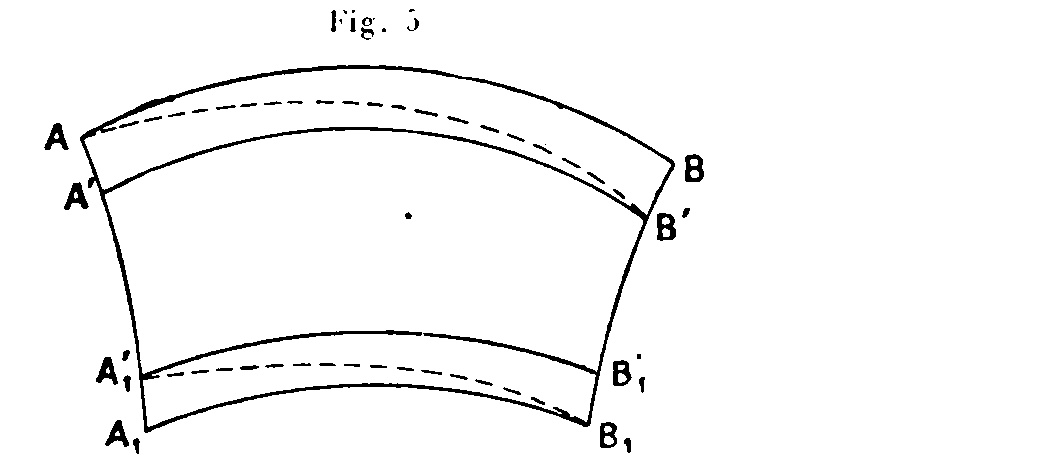
\includegraphics[width=0.55\textwidth]{fig5_scan.jpg}
\end{center}

Let $A'$ be a point near enough to A that the arc $AA'$ is without contact and that the characteristic $A'B'$ goes to cut $BB_1$ at a point $B'$ such that $BB'$ is without contact.

Suppose likewise that $A'_1B'_1$ is an arc of characteristic and that $A_1A'_1$, $B_1B'_1$ are without contact.

By the preceding theorem, one can draw algebraic arcs $AB'$, $A'_1B_1$ without contact.

The number of contacts of the algebraic cycle
\[
AB'B_1A'_1A
\]
must be even.

Now the characteristics AB, $A_1B_1$ touch the cycle at A and at $B_1$; the characteristics $A'B'$ and $A'_1B'_1$ cross it at $B'$ and at $A'_1$. Thus the four angular points count as an even number of contacts. Hence one has
\[
\begin{aligned}
&\text{number of contacts } AB' + \text{number of contacts } B'B_1\\
&\quad + \text{number of contacts } B_1A'_1 + \text{number of contacts } A'_1A \equiv 0 \pmod 2,
\end{aligned}
\]
or, what amounts to the same thing,
\[
\text{number of contacts } AA_1 + \text{number of contacts } BB_1 \equiv 0 \pmod 2.
\]
\hfill\mbox{Q. E. D.}

\emph{Theorem X.} --- \emph{If an arc of characteristic which passes through no singular point is subtended by an arc of curve, the number of contacts of this arc of curve is odd.}

Indeed, let $\mathrm F=0$ be the equation of the subtending arc. Consider the function $\mathrm F$; this function passes, for example, from positive to negative when the point $(x,y)$, describing the characteristic, passes through one of the endpoints of the subtending arc, and from negative to positive when it passes through the other endpoint of this arc. This means that, when the point $(x,y)$ describes the given arc of characteristic, the function $\mathrm F$ passes through an odd number of maxima and minima.

Now these maxima and minima are given by the equation
\[
\varphi=X\frac{d\mathrm F}{dx}+Y\frac{d\mathrm F}{dy}=0;
\]
that is, the arc of characteristic cuts the curve $\varphi=0$ in an odd number of points.

But this curve, being algebraic, cuts in an even number of points the cycle H formed by the arc of characteristic and the subtending arc; hence it cuts the subtending arc in an odd number of points.

Therefore the number of contacts of this arc is odd. \hfill\mbox{Q. E. D.}

\emph{Remark I.} --- If the arc of characteristic passes through a saddle, how must the theorem be modified?

The saddle evidently belongs to the curve $\varphi=0$, but it is a maximum or a minimum of $\mathrm F$ only on condition that the arc of characteristic has an angular point there.

Indeed, suppose first that there is no angular point. The curves $\mathrm F=\mathrm F(x_0,y_0)$ and $\varphi=0$ will both, in general, cross the cycle H; that is, the saddle will be a simple point of intersection of the cycle and of $\varphi=0$, without corresponding to a maximum or to a minimum of $\mathrm F$.

If, on the contrary, there is an angular point, one of the curves $\varphi=0$, $\mathrm F=0$ will cross the cycle H, while the other will touch it, so that either the saddle will be a simple point of intersection of H and of $\varphi=0$ and at the same time a maximum of $\mathrm F$, or else it will be a double point of H and of $\varphi=0$ without being a maximum of $\mathrm F$.

Thus, if the arc of characteristic passes through a saddle and has no angular point there, the number of contacts of the subtending arc is even.

If the arc of characteristic passes through a saddle and has an angular point there, the number of these contacts is odd.

\emph{Remark II.} --- One would prove in the same way that, if an arc of characteristic passes through no singular point, every arc of curve which subtends it has an even number of contacts.

\emph{Contacts of topographical systems.} --- If one considers an algebraic topographical system, the contacts of this system will form an algebraic curve.

One will distinguish the interior and exterior contacts of the topographical system, according as, in the neighborhood of these contacts, the characteristic passing through them remains inside or outside the cycle which it touches, among those of the topographical system.

The curve of contacts will therefore be divided into a certain number of arcs which will be the arcs of interior contacts and those of exterior contacts.

These arcs will be separated:

\begin{enumerate}[label=\arabic*°]
\item By the singular points;
\item By the points at which the curve of contacts touches one of the cycles of the topographical system.
\end{enumerate}


\ornament
\begin{center}
{\Large CHAPTER V.}\\[0.4em]
{\small THEORY OF CONSEQUENTS.}
\end{center}
\shortline

\emph{Fundamental convention.} --- Consider any semi-characteristic; we shall prolong it indefinitely if this can be done without encountering a singular point; if, on the contrary, in following the semi-characteristic we arrive at a node, we shall stop it at a node; if we arrive at a saddle, three paths will open before us when we wish to continue to follow the characteristic, the first in the prolongation of the path followed until then, the two others to the right and to the left; we shall agree to follow one of the paths to the right or to the left, without ever taking the one which is directly before us. For example, we shall consider OB or OD (fig. 6), and not OC, as the prolongation of AO.

\figscan{6}{0.48\textwidth}

In this way one may say that in the neighbourhood of a saddle there are four characteristics glued one against another, and having, two by two, a common branch: these are the characteristics AOB, BOC, COD, DOA.

\emph{Definition of consequents.} --- Let
\[
x=\varphi(t),\qquad y=\psi(t)
\]
be an algebraic arc without contact; $\varphi$ and $\psi$ are algebraic functions of $t$, and have only one value for each value of $t$. The extremities of the arc will correspond to the values of $t$,
\[
t=\alpha,\qquad t=\beta.
\]

Such an arc, without contact, will have two sides, which we shall call its right and its left; a point infinitely near the arc AB can, in fact, be to the right or to the left of this arc. For example, the point $m$ will be to the left of the arc AB (fig. 7), the point $m'$ to the right of the arc AB, because one cannot pass from one to the other without crossing the arc AB, or without moving away from this arc by a finite distance, or without passing through a circle of infinitely small radius drawn with A or with B as centre.

\figscan{7}{0.44\textwidth}

This being so, consider any point $\mathrm M_0$ of the arc AB (fig. 8); from this point issue two semi-characteristics, one toward the left, the other toward the right of the arc AB; let us consider the one on the left.

\figscan{8}{0.55\textwidth}

Several cases may arise:
\begin{enumerate}[label=\arabic*°]
\item This semi-characteristic may be prolonged indefinitely, without again meeting the arc AB.
\item This semi-characteristic ends by turning around a focus, before having again met the arc AB.
\item It ends at a node where we must stop it, according to the fundamental convention, and this before having again met the arc AB.
\end{enumerate}

In these first three cases, we shall say that \emph{the point $\mathrm M_0$ has no consequent.}

\begin{enumerate}[label=\arabic*°,start=4]
\item The semi-characteristic comes to meet the arc AB at $\mathrm M_1$ before having passed through a singular point. We shall then say that \emph{the point $\mathrm M_1$ is the consequent of the point $\mathrm M_0$.}
\item The semi-characteristic reaches a saddle before it has arrived at again meeting the arc AB. In this case, according to the fundamental convention, one must turn either to the right or to the left, and each of these two paths may lead us or may not lead us to meet the arc AB again. The point $\mathrm M_0$ may then have $0$, $1$, or $2$ consequents.
\end{enumerate}

It may finally happen that the semi-characteristic meets two saddles or still more; in that case the point $\mathrm M_0$ could have more than two consequents.

If, starting from the point $\mathrm M_0$, instead of considering the semi-characteristic on the left, one had considered that on the right, one could have arrived at a point $\mathrm M'$ situated on the arc AB.

\emph{This point $\mathrm M'$ will be called the antecedent of the point $\mathrm M_0$.}

Under these conditions, the point $\mathrm M_0$ will itself be the antecedent of its consequent $\mathrm M_1$.

If $t_0$ and $t_1$ are values of $t$ corresponding to $\mathrm M_0$ and to $\mathrm M_1$, the law of consequence will be the relation that connects $t_0$ with $t_1$.

\emph{Theorem XI.} --- \emph{If $t_0=t_1$, the characteristic is a cycle. If $t_0\gtrless t_1$, the characteristic is a spiral.}

Indeed, the first part of the statement is a genuine tautology. The second is proved easily in the following way.

First note that the arc $\mathrm M_0\mathrm D\mathrm M_1$ (fig. 9) subtends the arc $\mathrm M_0\mathrm C\mathrm M_1$ of the characteristic, since it is without contact.

Moreover, this arc $\mathrm M_0\mathrm D\mathrm M_1$ cannot meet the characteristic at any point other than $\mathrm M_0$ and $\mathrm M_1$. For arcs such as $\mathrm M_1\mathrm F\mathrm M_2$, $\mathrm M_0\mathrm H\mathrm M_3$ would be subtended by the arcs $\mathrm M_1\mathrm M_2$, $\mathrm M_0\mathrm M_3$, which is impossible, since these arcs are supposed to be without contact.

\figscan{9}{0.6\textwidth}

This being so, through the point $\mathrm N_0$, infinitely near $\mathrm M_0$ and to the left of the latter, one can draw an arc of characteristic $\mathrm N_0\mathrm E\mathrm N_1$ which will come to meet the arc $\mathrm M_0\mathrm M_1$ at a point $\mathrm N_1$ infinitely near $\mathrm M_1$ and to the left of the latter, for it could not pass to the right without cutting the characteristic $\mathrm M_0\mathrm C\mathrm M_1$, which is impossible.

The cycle $\mathrm N_1\mathrm M_0\mathrm N_0\mathrm E\mathrm N_1$ therefore meets the characteristic $\mathrm M_0\mathrm C\mathrm M_1$ only at a single point, namely $\mathrm M_0$. Therefore this characteristic is a spiral. \hfill\mbox{Q. E. D.}

\emph{Theorem XII.} --- \emph{Every characteristic that does not end at a node is a cycle or a spiral.}

Indeed, if this characteristic meets no algebraic cycle in an infinity of points, it is a cycle, by theorem I.

If, on the contrary, it meets an algebraic cycle in an infinity of points, since this cycle is composed of a finite number of arcs without contact, it will meet one of these arcs, and will have contact at more than one point; that is to say, one of the points of intersection will have a consequent.

If it coincides with its consequent, the characteristic is a cycle; if it does not coincide with its consequent, the characteristic is a spiral, by theorem XI.

The theorem is therefore proved.

\emph{Theorem XIII.} --- \emph{If $\mathrm M_0$ does not correspond to a characteristic passing through a saddle, and if it has a consequent $\mathrm M_1$; if $t_1=\varphi_1(t_0)$ is the law of consequence, the function $\varphi_1$ is holomorphic for the values of $t_0$ near the one that corresponds to $\mathrm M_0$.}

Indeed, we supposed at the beginning that if
\[
x=\varphi(t),\qquad y=\psi(t)
\]
are the equations of the arc without contact, $\varphi$ and $\psi$ are holomorphic functions of $t$ in the neighbourhood of the value of $t$ that corresponds to $\mathrm M_0$, and also of the one that corresponds to $\mathrm M_1$.

Suppose that one seeks an integral of the partial-difference equation
\[
X\frac{dz}{dx}+Y\frac{dz}{dy}=0,
\]
which is constrained to reduce identically to $t_0$ when one sets
\[
x=\varphi(t_0),\qquad y=\psi(t_0).
\]

This integral represents a surface that passes through the skew curve
\[
x=\varphi(z),\qquad y=\psi(z).
\]

In the neighbourhood of the point $\mathrm M_0$, this integral is holomorphic in $x$ and in $y$, for the arc
\[
x=\varphi(t_0),\qquad y=\psi(t_0)
\]
does not touch a characteristic.

It will likewise be holomorphic in $x$ and in $y$ all along the characteristic that passes through the point $\mathrm M_0$, unless this characteristic passes through a singular point. Now we have supposed that this characteristic was going to pass through the point $\mathrm M_1$ without having met any singular point. In the neighbourhood of the point $\mathrm M_1$, $z$ is therefore a holomorphic function of $x$ and $y$; and, if one there sets
\[
x=\varphi(t_1),\qquad y=\psi(t_1),
\]
$z$ becomes a holomorphic function of $t_1$, in the neighbourhood of the value of $t_1$ corresponding to $\mathrm M_1$.

Now $z$ is nothing other than $t_0$. Therefore $t_0$ is a holomorphic function of $t_1$. One would prove identically, in the same way, that $t_1$ is a holomorphic function of $t_0$ in the neighbourhood of the value of $t_0$ corresponding to $\mathrm M_0$.

\emph{Corollary I.} --- The function $t_1=\varphi_1(t_0)$, which expresses the law of consequence, can present a discontinuity only for the values of $t_0$ that correspond to characteristics passing through saddles.

\emph{Corollary II.} --- If one divides the arc without contact AB into partial arcs, such that all the points of each of these arcs have a consequent, or none has one, the extremities of these partial arcs will be points having as consequent an extremity of the arc without contact AB, or corresponding to characteristics passing through saddles.

\emph{Corollary III.} --- If the extremities of the arc without contact correspond to the values
\[
t=\alpha,
\qquad
 t=\beta;
\]
if, for no value of $t$ such that
\[
\alpha<t<\beta,
\]
the corresponding characteristic passes through a saddle;

if, for all values of $t$ such that ($\alpha_1$ and $\beta_1$ being given constants) one has
\[
\alpha<\alpha_1<t<\beta_1<\beta,
\]
the corresponding characteristic is a cycle;

the characteristics that correspond to any value whatsoever of $t$ comprised between $\alpha$ and $\beta$ are all cycles.

\emph{Theorem XIV.} --- \emph{The value of $\dfrac{dt_1}{dt_0}$ is always positive.}

Indeed, let AB be the arc without contact (fig. 11), let $\mathrm M_0\mathrm M_1$ be a characteristic,

\figscan{10}{0.48\textwidth}

and let $\mathrm N_0$ be a point infinitely near $\mathrm M_0$ and situated to the right of this point. Let $\mathrm N_0\mathrm N_1$ be the characteristic passing through this point. The point $\mathrm N_1$ is infinitely near $\mathrm M_1$; I say that it is to the right of this point. For, in order for it to be to the left, the characteristic $\mathrm N_0\mathrm N_1$ would have to leave the cycle $\mathrm M_0\mathrm H\mathrm M_1\mathrm N_0\mathrm M_0$ when it is prolonged beyond $\mathrm N_1$, that is to say, the arc of characteristic $\mathrm N_0\mathrm N_1$ would have to be subtended by the arc $\mathrm N_0\mathrm N_1$, which is impossible, since this arc is without contact.

\emph{Study of the curve of consequence.} --- If one regards the quantities $t_0$ and $t_1$ as the coordinates of a point, the law of consequence
\[
t_1=\varphi_1(t_0)
\]
represents a curve. This curve is entirely contained in the square
\[
\begin{array}{ll}
t_0=\alpha, & t_1=\alpha,\\
t_0=\beta, & t_1=\beta.
\end{array}
\]

\emph{First case.} --- To no value of $t$ comprised between $\alpha$ and $\beta$ corresponds a characteristic that goes through a saddle.

In this case, the curve of consequence is continuous; it meets the parallels to the axes at only one point; following the curve in a suitable direction, one constantly moves away from these two axes.

This is to say that if KLCD is the square (fig. 11)
\[
\begin{array}{ll}
t_0=\alpha, & t_1=\alpha,\\
t_0=\beta, & t_1=\beta,
\end{array}
\]
the curve presents forms such as
\[
\mathrm{AB},\quad \mathrm{CD},\quad \mathrm{EF},\quad \mathrm{GH}.
\]

\figscan{11}{0.45\textwidth}

It will represent the form CD when the values $\alpha$ and $\beta$ of $t_0$ correspond to cycles, while no value of $t_0$ comprised between $\alpha$ and $\beta$ corresponds to a cycle.

\emph{Second case.} --- Suppose that to certain values $\gamma_0$, $\gamma'_0$, \ldots{} of $t_0$ comprised between $\alpha$ and $\beta$ there correspond characteristics going through a saddle;

that, moreover, to the values $\alpha$ and $\beta$ there correspond cycles; that to no intermediate value there corresponds a cycle:

From all saddles issue four branches of characteristics; some of these branches come to meet the given arc without contact; others do not.

Suppose first that all those of these branches which come to meet the given arc without contact issue from one and the same saddle:

$1^\circ$ It is impossible for the four branches issuing from the same saddle to go and meet the arc without contact. Let, indeed, AB (fig. 12) be the given arc without contact

\figscan{12}{0.5\textwidth}

Let C be the given saddle; let $\mathrm C\mathrm M_0$, $\mathrm C\mathrm M_1$, $\mathrm C\mathrm N_0$, $\mathrm C\mathrm N_1$ be the four branches of characteristics that issue from this saddle, in such a way that $\mathrm M_1\mathrm C\mathrm M_0$, $\mathrm N_1\mathrm C\mathrm N_0$, do not form an angular point.

According to theorem X, remark I, the portion $\mathrm M_0\mathrm M_1$ of the arc AB subtends the characteristic $\mathrm M_0\mathrm C\mathrm M_1$.

The two arcs $\mathrm A\mathrm M_0$, $\mathrm M_1\mathrm B$ are therefore on the same side of the cycle $\mathrm M_0\mathrm M_1\mathrm C\mathrm M_0$; let us call this side of the cycle the exterior of the cycle. The two branches of curve $\mathrm C\mathrm N_0$, $\mathrm C\mathrm N_1$ are one on the exterior, the other on the interior of the cycle $\mathrm M_0\mathrm M_1\mathrm C\mathrm M_0$. Let $\mathrm C\mathrm N_1$ be the one that is on the interior; it could meet the arc AB only between $\mathrm M_0$ and $\mathrm M_1$, and on the same side as the branches of curve $\mathrm C\mathrm M_0$, $\mathrm C\mathrm M_1$, so that the algebraic arc $\mathrm M_1\mathrm N_1$ would subtend the arc of characteristic $\mathrm M_1\mathrm C\mathrm N_1$, which is impossible by theorem X.

\emph{Remark I.} --- The hypothesis that we made at the outset is therefore absurd. \hfill\mbox{Q. E. D.}

$2^\circ$ It may happen that three of the branches issuing from the same saddle meet the arc without contact. In this case, either there is a point that has two consequents and the points situated between these two consequents have no antecedent; or else there is a point that has two antecedents, and the points situated between these two antecedents have no consequent.

In such a way the curve of consequence assumes either the form CHFD or the form CABD (fig. 13).

\figscan{13}{0.42\textwidth}

$3^\circ$ It cannot happen that two or only one of the branches issuing from the same saddle meet the arc without contact.

Indeed, suppose first that there are two branches of characteristics $\mathrm C\mathrm M_0$ and $\mathrm C\mathrm M_1$ that meet AB, and that $\mathrm M_0\mathrm C\mathrm M_1$ (fig. 14) presents an angular point

\figscan{14}{0.48\textwidth}

at C. A point infinitely near $\mathrm M_0$ will have a consequent if it is to the right of $\mathrm M_0$, and will not have one if it is to the left. Therefore, according to corollary II of theorem XIII, the points of the arc $\mathrm M_0\mathrm A$ will therefore have no consequent. A point infinitely near A would therefore have no consequent, which is absurd, since A is its own consequent. Similarly, if one supposed that $\mathrm M_1\mathrm C\mathrm M_0$ presents no angular point, or that $\mathrm C\mathrm M_1$ does not meet the arc AB, one would arrive at this absurd result, that a point infinitely near A has no consequent. The hypotheses made at the beginning are therefore equally absurd. \hfill\mbox{Q. E. D.}

We shall not examine in detail the cases in which the branches of characteristics that come to meet the arc without contact issue from several different saddles. The discussion would be made according to the same principles; it would merely be longer. Let us cite only a few examples of possible combinations\footnote{It follows from the text that the author had in view a second example, corresponding to the representative curve CEFGHD. In this case, the arc without contact is met by three branches of characteristics issuing from a first saddle, and by three branches issuing from a second saddle. (R. G.)}.

$1^\circ$ \emph{Curve} CABD (fig. 15). --- The arc without contact is met by two

\figscan{15}{0.42\textwidth}

branches of characteristics issuing from a first saddle $\lambda$ and by two branches issuing from a second saddle $\mu$. These two systems of two branches of characteristics each present an angular point, one at $\lambda$, the other at $\mu$.

If one makes $t_0$ vary from $\alpha$ to the value corresponding to the point A and to the characteristic passing through $\lambda$, one has a consequent; then, as $t_0$ varies from the value corresponding to the point A to the one corresponding to the point B and to the characteristic passing through $\mu$, one no longer has a consequent; and one has one again when $t_0$ varies from the value corresponding to B up to $\beta$.

\ornament
\begin{center}
{\Large CHAPTER VI.}\\[0.4em]
{\small THEORY OF LIMIT CYCLES.}
\end{center}
\shortline

From what we have seen above, the characteristics can be divided into four categories:
\begin{enumerate}[label=\arabic*°]
\item Cycles;
\item Spirals that can be followed indefinitely in both directions without ending at a node or turning about a focus, and without returning to the starting point;
\item Characteristics that can be followed indefinitely in one direction without encountering a node or approaching a focus, but which, in the other direction, end at a node or approach a focus indefinitely;
\item Those which end on both sides at a node or at a focus.
\end{enumerate}

By the same principles, the \emph{half-characteristics} are divided into four categories:
\begin{enumerate}[label=\arabic*°]
\item Cycles;
\item Half-spirals that are followed along an infinite arc without arriving at a node or at a focus and without returning to the starting point;
\item Half-characteristics that end at a node;
\item Those that turn indefinitely about a focus.
\end{enumerate}

According to Theorem I, the half-characteristics of the second category meet certain algebraic cycles, and consequently certain contact-free algebraic arcs, in infinitely many points.

Let AB be one of these contact-free algebraic arcs.

Let $\mathrm M_0$ (fig. 16) be the point from which the half-characteristic under consideration issues.

\figscan{16}{0.62\textwidth}

Let $\mathrm M_1$ be the consequent of $\mathrm M_0$, and suppose that $\mathrm M_1$ is to the right of $\mathrm M_0$.

Let $\mathrm M_2$ be the consequent of $\mathrm M_1$, $\mathrm M_3$ that of $\mathrm M_2$, and so on; $\mathrm M_2$ will be to the right of $\mathrm M_1$, $\mathrm M_3$ to the right of $\mathrm M_2$, and so on.

In general, $\mathrm M_{n+1}$ will be to the right of $\mathrm M_n$, and, since, however large $n$ may be, $\mathrm M_n$ is always on the arc AB, $\mathrm M_n$ will tend to a limit as $n$ increases indefinitely. Let H be this limit.

The consequent of $\mathrm M_n$, when $n$ is infinitely large, is infinitely close to $\mathrm M_n$. Therefore H is its own consequent; therefore the characteristic passing through H is a cycle; we shall call it the \emph{limit cycle} of the given half-characteristic. One can follow, on the characteristic passing through $\mathrm M_0$, an arc sufficiently large to approach the point H as closely as desired.

Let HK be an arc of the characteristic passing through the point H. Let CD be an algebraic arc passing through K.

One can take $n$ large enough so that the arc of characteristic issuing from $\mathrm M_n$ meets CD.

Suppose, for example, that the arc issuing from $\mathrm M_2$ meets CD at $\mathrm N_2$. The arc issuing from $\mathrm M_3$ will meet CD at $\mathrm N_3$, ... the arc issuing from $\mathrm M_n$, at a point $\mathrm N_n$.

$\mathrm N_3$ will be to the right of $\mathrm N_2$, ..., $\mathrm N_{n+1}$ will be to the right of $\mathrm N_n$. Thus the given half-characteristic will meet CD in infinitely many points $\mathrm N_2$, $\mathrm N_3$, ..., $\mathrm N_n$, and $\mathrm N_n$ will tend to K as $n$ increases indefinitely.

In summary, every half-characteristic of the second category has a limit cycle.

Every algebraic arc, however small it may be, that cuts this cycle cuts the half-characteristic in infinitely many points.

One can find a point of the half-characteristic as close as desired to an arbitrary point of its limit cycle.

Let AB (fig. 17) be a contact-free algebraic arc. Suppose that to no

\figscan{17}{0.45\textwidth}

point M situated between A and B there corresponds a characteristic passing through a saddle; that to the point $\mathrm M_0$ there corresponds a limit cycle; and that to no point M different from $\mathrm M_0$, situated between A and B, there corresponds a limit cycle. Every characteristic that meets AB will have as its limit cycle the cycle passing through $\mathrm M_0$.

If one considers a limit cycle C (fig. 18) which does not pass through a saddle and which passes through a point $\mathrm M_0$, one can draw through $\mathrm M_0$ an algebraic arc AB small enough to be contact-free; so that between A and $\mathrm M_0$, or between $\mathrm M_0$ and B, there is no point to which there corresponds a characteristic passing through a saddle or a limit cycle. All the characteristics that meet AB then have C

\figscan{18}{0.47\textwidth}

as their limit cycle, so that C is the limit cycle of two series of characteristics, one situated inside the cycle and the other outside it.

Let us see what happens when C comes to pass through a saddle.

Let H be the saddle, and let HA, HB, HC, HD be the four branches of characteristics issuing from this saddle. Suppose that two of these branches, HA and HB for example, end at the same point M, so as to form a cycle HAMBH; this cycle will always be the limit cycle of curves such as $\alpha\alpha$; inspection of the figure shows this (fig. 19).

\figscan{19}{0.75\textwidth}

Consider, on the contrary, the curve $\beta\beta$; it is easy to see that, if the branches of curve HC, HD do not end at the same point N, the cycle HAMBH is not the limit cycle of $\beta\beta$.

If, on the contrary, HC and HD reunite at N, then $\beta\beta$ has as limit cycle the polycycle
\[
\mathrm{HAMBHDNCH}.
\]

\emph{Theorem XV.} --- \emph{Inside and outside any limit cycle, there is always at least one focus or one node.}

To prove this theorem we shall call \emph{tangencies of a cycle} the points where it touches one of the great circles $x=\mathrm{const.}$

The tangencies will be direct if, in the neighborhood of the point of contact, the tangent great circle remains outside the cycle. They will be inverse in the contrary case.

We shall next prove the following two lemmas:

\emph{Lemma I.} --- \emph{If the points of intersection of the equator with the great circle $x=0$, points that we shall call $m$, $m'$, are both outside a cycle, the excess of the number of direct tangencies of this cycle over the number of its inverse tangencies is 2.}

If the points $m$, $m'$ are both inside the cycle, this excess is $-2$.

If the points $m$, $m'$ are one outside and the other inside, this excess is 0.

Indeed, one can pass from any cycle A to any other cycle B by continuous deformation, that is, by passing from the cycle A to a cycle differing from it by an infinitesimal amount, A', and then by a series of cycles C differing infinitesimally from one another, one will arrive at a cycle B', differing infinitesimally from B.

In these successive deformations, a direct tangency will never be transformed into an inverse tangency, nor an inverse tangency into a direct tangency, for this could occur only if one of the great circles $x=\mathrm{const.}$ became osculating to one of the cycles; in that case, two tangencies, one direct and the other inverse, would have come to coincide, and, in that case, they would generally disappear for one of the cycles infinitesimally near C.

The excess to be evaluated in this lemma can be modified in these continuous deformations of the cycle only if two of the tangencies come to coincide and then disappear. This can occur in two cases:

$1^\circ$ When one of the cycles C comes to pass through one of the points $m$, $m'$; but we shall suppose: $1^\circ$ that the points $m$, $m'$ are both inside A and both outside B; $2^\circ$ or that the points $m$, $m'$ are both outside A and outside B; $3^\circ$ or that $m$ is outside A and B while $m'$ is inside these two cycles; and consequently one will always have been able to choose the series of cycles C that allow passage from the cycle A to the cycle B in such a way that none of the cycles C passes either through $m$ or through $m'$.

$2^\circ$ This can also occur if one of the cycles C becomes osculating to one of the circles $x=\mathrm{const.}$ But in this case it is a direct tangency and an inverse tangency that coincide and disappear. The excess to be evaluated is therefore not modified.

Thus this excess is the same for A and for B.

But suppose that A is an arbitrary convex cycle, and B the given cycle.

The excess in question will be 2 for A if $m$ and $m'$ are outside A; it will be $-2$ if they are both inside, and 0 if one is inside and the other outside.

The excess in question will therefore be, for B, 2, $-2$, and 0 under the same conditions.

The lemma is therefore proved.

\emph{Lemma II.} --- \emph{If one traverses a cycle so as always to have the interior on one's left and observes the variations of the angular coefficient $\frac{dy}{dx}$, one will observe that at each direct tangency, $\frac{dy}{dx}$ will jump from $+\infty$ to $-\infty$ if one is in the first hemisphere, and from $-\infty$ to $+\infty$ if one is in the second hemisphere, and that the contrary holds for inverse tangencies.}

\emph{Proof of the theorem.} --- First suppose that the limit cycle under consideration is such that the two points $m$ and $m'$ are on the same side of this cycle, the side that we shall call the \emph{outside of the cycle}.

Let:

$\nu$ be the number of nodes and foci contained inside the cycle;

$\nu'$ the number of nodes and foci situated outside the cycle;

$\gamma$ and $\gamma'$ the numbers of saddles situated inside and outside this cycle.

One has
\[
\nu+\nu'-\gamma-\gamma'=2.
\]

The cycle cuts the equator in a certain number of points, in such a way that it can be divided into a certain number of secondary cycles, some lying entirely in the first hemisphere and the others entirely in the second hemisphere, and formed with arcs of the primitive cycle and arcs of the equator.

Suppose, to fix ideas, that the given cycle is the cycle ALDKCGBHA, which cuts the equator at the points A, B, C, D (fig. 20). The cycle decomposes

\figscan{20}{0.62\textwidth}

into three secondary cycles:
\[
\mathrm{AEBHA},\qquad \mathrm{CFDKC},\qquad \mathrm{CGBEALDFC}.
\]

Now, according to Theorem IV, one has
\[
-(\nu-\gamma)=\operatorname{ind.}\mathrm{AEBHA}+\operatorname{ind.}\mathrm{CFDKC}+\operatorname{ind.}\mathrm{CGBEALDFC}.
\]

Let $\alpha$, $\alpha'$, $\alpha''$, $\alpha'''$ be the number of direct tangencies of the arcs AHB, CKD, CGB, ALD; $\beta$, $\beta'$, $\beta''$, $\beta'''$ the number of their inverse tangencies; let $\lambda$ and $\lambda'$ be the number of times that $\frac{Y}{X}$ jumps from $-\infty$ to $+\infty$ when the arcs AEB and CFD are traversed; and $\mu$ and $\mu'$ the number of times that $\frac{Y}{X}$ jumps from $+\infty$ to $-\infty$ when the arcs AEB and CFD are traversed. We have, by virtue of Lemma II and noting that all along the given cycle one has
\[
\frac{dy}{dx}=\frac{Y}{X},
\]
\[
\begin{aligned}
2\operatorname{ind.}\mathrm{AEBHA}&=-\alpha+\lambda-\mu+\beta,\\
2\operatorname{ind.}\mathrm{CFDKC}&=-\alpha'+\lambda'-\mu'+\beta',\\
2\operatorname{ind.}\mathrm{CGBEAL}&=-\alpha''-\alpha'''+\beta''+\beta'''-\lambda-\lambda'+\mu+\mu'.
\end{aligned}
\]
whence
\[
-(2\nu-2\gamma)=\beta+\beta'+\beta''+\beta'''-\alpha-\alpha'-\alpha''-\alpha''',
\]
or, according to Lemma I,
\[
-(2\nu-2\gamma)=-2,\qquad \nu-\gamma=1.
\]
We therefore also have
\[
\nu'-\gamma'=1,
\]
whence
\[
\nu>0,\qquad \nu'>0.
\]
\hfill\mbox{Q. E. D.}

In the cases where the points $m$, $m'$ lie on opposite sides of the cycle, the difficulty is easy to avoid. Indeed, one will always find on the sphere two diametrically opposite points that are on the same side of the cycle, and a change of variables will suffice to reduce to the preceding case.

If one does not find on the sphere two diametrically opposite points that are on the same side of the cycle, it is because the points of the cycle are pairwise diametrically opposite, that is, because the cycle is symmetric to itself with respect to the center of the sphere, and then the theorem is evident by itself.

\emph{Theorem XVI.} --- \emph{An algebraic cycle that passes through all the nodes and all the foci meets all limit cycles.}

Indeed, let C be any limit cycle; it contains certain nodes and certain foci in its interior, and certain nodes and certain foci in its exterior.

There are therefore points of the given algebraic cycle that are outside C, and others that are inside, that is, the given algebraic cycle meets C. \hfill\mbox{Q. E. D.}

\emph{Corollary.} --- Every algebraic cycle that passes through all the nodes and all the foci meets all the characteristics.

\emph{Theorem XVII.} --- \emph{The limit cycles are finite in number, provided that none of them passes through a saddle.}

Indeed, pass an algebraic cycle C through all the nodes and all the foci. Let
\[
x=\varphi(t),\qquad y=\psi(t)
\]
be the equations of this cycle C.

This cycle C, meeting all the limit cycles, would have infinitely many points of intersection with these limit cycles if they were infinite in number. There would therefore be a point of this cycle C around which these points of intersection would be infinitely close, that is, if
\[
t_1=\varphi_1(t_0)
\]
is the law of consequence of a certain contact-free arc of the cycle C, there will be a certain value $\tau$ of $t_0$ such that, as $t_0$ varies from $\tau-\varepsilon$ to $\tau+\varepsilon$, $t_1$ becomes equal to $t_0$ infinitely many times.

But if $\tau$ does not correspond to a characteristic passing through a saddle, $\varphi(t_0)$ is holomorphic for $t_0=\tau$, and therefore one cannot have, infinitely many times ($t_0$ varying from $\tau-\varepsilon$ to $\tau+\varepsilon$),
\[
t_0=\varphi(t_0).
\]

Nor can this happen if $\tau$ does not correspond to a limit cycle.

Thus there can be infinitely many limit cycles only if one of them passes through a saddle.

\emph{Theory of limit annuli.} --- Let there again be an algebraic cycle C passing through all the nodes and all the foci. One can cut from it a certain number of contact-free arcs containing all the points that correspond to limit cycles and containing none of the points that correspond to characteristics passing through saddles.

Let $t_1=\varphi(t_0)$ be the law of consequence of one of these arcs, and suppose that $t_0$ is made to vary from $\alpha$ to $\beta$; that the points $t_0=\alpha$, $t_0=\beta$ have two

\figscan{21}{0.56\textwidth}

consequents $t_1=\alpha'$, $t_1=\beta'$. Let $\mathrm A_1$ be the point of the contact-free arc that corresponds to $t_0=\tau$. Suppose that one considers the point of the sphere lying on the characteristic that passes through $\mathrm A_1$ and separated from $\mathrm A_1$ by an arc $s$ of characteristic, and that to this point one makes correspond a point of the plane whose coordinates are $s$ and $\tau$ (fig. 21).

To the contact-free arc there will correspond:

$1^\circ$ The segment of the line $s=0$ comprised between the points
\[
\tau=\alpha,\qquad \tau=\beta,\qquad \mathrm{namely}\quad \mathrm{AB}\ (\text{fig. }21);
\]

$2^\circ$ A certain arc of curve CD, defined by the equation
\[
s=\lambda(\tau),
\]
where $\lambda(\tau)$ is the length of the characteristic passing through $\mathrm A_1$ that must be traversed before meeting the contact-free arc again.

An arbitrary point of the contact-free arc will be represented by a point $\mathrm B_i$ of the segment AB and by a point $\mathrm D_i$ of the arc CD. Every arc of curve going from $\mathrm D_i$ to $\mathrm B_i$ represents a cycle; this cycle will be contact-free if the arc of curve $\mathrm D_i\mathrm B_i$ is not tangent to any of the lines $\tau=\mathrm{const.}$

Now it is clear that one can join by straight lines A and C, B and D, then foliate the mixtilinear quadrilateral ABCD by arcs of curve that are tangent to none of the lines $\tau=\mathrm{const.}$ and that do not meet at any point.

\emph{Consequence.} --- Around any limit cycle there is an annular region bounded by two contact-free cycles that we shall call \emph{boundary cycles}, and foliated by contact-free cycles that do not meet at any point.

These annular regions will be called \emph{limit annuli} and will be finite in number.

Around the nodes and the foci, one can likewise draw a series of contact-free cycles enveloping one another, so that the nodes and the foci also have their limit annuli.

We have implicitly supposed that no limit cycle passed through a saddle, for we considered on the algebraic cycle C arcs on which lay all the points corresponding to limit cycles, and on which lay none of the points corresponding to characteristics passing through saddles.

Now suppose that a limit cycle passes through a saddle; we know that two cases can occur:

$1^\circ$ Such a characteristic is the limit cycle only of characteristics that are sufficiently near it and situated inside the cycle (see fig. 19). In this case, one will cut on the cycle C a contact-free arc, bounded at the point that corresponds to the limit cycle passing through a saddle, and containing no other point corresponding to a characteristic passing through a saddle; and, reasoning as in the general case, one will see that the cycle passing through a saddle also has a limit annulus, but one of which it is itself the boundary cycle.

$2^\circ$ The cycles HAMBH, HCNDH (fig. 19) are limit cycles of the characteristics situated inside these cycles, while the polycycle HAMBHDNCH is the limit cycle of the exterior characteristics.

Reasoning as in the first special case, one would see that each of these three cycles has a limit annulus, of which it is itself the boundary cycle; so that these three limit annuli form, by their juxtaposition, a single annular region.

\emph{Interannular regions.} --- The boundary cycles divide the sphere into two categories of regions: $1^\circ$ the limit annuli that we have just studied; $2^\circ$ the interannular regions.

A moving point traveling along a characteristic with uniform speed and starting from a point situated in an interannular region will, after a finite time, cross a boundary cycle and pass into a limit annulus.

\figscan{22}{0.62\textwidth}

For the interannular regions contain neither node nor focus nor any point of the limit cycles.

I say that the interannular regions are, like the limit annuli, foliated by contact-free cycles. Indeed, suppose, to fix ideas, that an interannular region is bounded by three boundary cycles A, B, C and divided into two parts, foliated, the first by characteristics going from A to B, the second by characteristics going from A to C. The two parts of the region must be separated by a characteristic passing through a saddle D (fig. 22). Let $\alpha D$, $\alpha'D$, $\beta D$, $\beta'D$ be the four branches of characteristics issuing from D.

Let $\tau$ be any parameter defining a point $\lambda_1$ of the cycle A. Let $(x,y)$ be a point of a characteristic issuing from $\lambda_1$, and let $s$ be the arc of characteristic separating $(x,y)$ from $\lambda_1$. Represent the point of the sphere $(x,y)$ by the point of the plane whose coordinates are $s$ and $\tau$. The line $\mathrm A_1\mathrm C_1\mathrm B_1$ ($s=0$) (fig. 23)

\figscan{23}{0.55\textwidth}

will represent the cycle A; $\mathrm A_1$ and $\mathrm B_1$ will represent the point $\alpha$; $\mathrm C_1$ will represent the point $\alpha'$; the arcs $\mathrm E_4\mathrm E_3$, $\mathrm E_2\mathrm E_1$ will represent respectively the cycles B and C; $\mathrm D_1$, $\mathrm D_2$, $\mathrm D_3$ will represent the point D; $\mathrm E_4$ and $\mathrm E_3$ will represent $\beta$; $\mathrm E_2$ and $\mathrm E_1$ will represent $\beta'$. Moreover, one will have
\[
\mathrm E_4\mathrm D_3=\mathrm E_3\mathrm D_1,\qquad
\mathrm E_2\mathrm D_1=\mathrm E_1\mathrm D_2,\qquad
\mathrm A_1\mathrm D_3=\mathrm B_1\mathrm D_2.
\]

The arcs of curve $\alpha\beta\gamma$, $\delta\varepsilon$, $\zeta\theta$, where one has
\[
\begin{array}{lll}
\mathrm A_1\alpha<\mathrm A_1\mathrm D_3, & \beta\mathrm C_1<\mathrm D_1\mathrm C_1, & \mathrm A_1\alpha=\mathrm B_1\gamma,\\
 & \varepsilon\mathrm C_1>\mathrm D_1\mathrm C_1, & \varepsilon\mathrm D_1=\delta\mathrm D_3,\\
 & \zeta\mathrm C_1>\mathrm D_1\mathrm C_1, & \theta\mathrm D_2=\zeta\mathrm D_1,
\end{array}
\]
represent cycles, and these cycles will be contact-free if the arcs $\alpha\beta\gamma$, $\delta\varepsilon$, $\zeta\theta$ have no tangent parallel to the $s$-axis. Now it is clear that one can foliate the mixtilinear polygon $\mathrm A_1\mathrm B_1\mathrm E_1\mathrm E_2\mathrm E_3\mathrm E_4$ by arcs satisfying this condition. Thus one can foliate the interannular region by contact-free cycles, which allows the following theorem to be stated:

\emph{Theorem XVIII.} --- \emph{There always exists a topographic system formed of contact-free cycles, contact-free polycycles, and limit cycles. This topographic system foliates the whole surface of the sphere. The bottoms and the summits are the nodes and the foci of the given equation. The saddles are the saddles of the given equation.}

Knowledge of this topographic system makes it possible to discuss completely the forms assumed by the curves defined by the given differential equation. This will be better understood, moreover, from the examples that follow.

\ornament

\begin{center}
{\Large CHAPTER VII.}\\[0.4em]
{\small EXAMPLES OF COMPLETE DISCUSSIONS.}
\end{center}
\shortline

\emph{First example.} --- Let (Fig. 24) the equation be
\[
\frac{dy}{xy-1}=\frac{dx}{1-x^2-y^2}.
\]

One may first observe that the curves $\mathrm X=0$, $\mathrm Y=0$, which are, respectively,
\[
xy=1,
\]
and
\[
x^2+y^2=1,
\]
do not meet at any point, either away from the equator or on the equator.

If, moreover, $X_2$ and $Y_2$ are the terms of the second degree of $X$ and of $Y$, one has
\[
X_2=-(x^2+y^2),\qquad Y_2=xy,
\]
\[
xY_2-yX_2=y(2x^2+y^2).
\]

The expression $xY_2-yX_2$ vanishes only for $y=0$.

Thus the equation has no singular point away from the equator, and on the equator itself it has two, which are at the intersection of the equator with the great circle $y=0$, and which are evidently nodes.

The equator, passing through all the singular points, meets all the limit cycles; but, since it is a characteristic and passes through no saddle, it can meet no other characteristic at any point other than the two nodes N and N$'$; it therefore meets no limit cycle: hence there is no limit cycle; hence all the characteristics start from N and end at N$'$.

Figure 24 represents the stereographic projection of the first hemisphere.

\figscan{24}{0.55\textwidth}

NBN$'$B is the equator; NN$'$ are the nodes; NAN$'$, NA$'$N$'$ are characteristics.

\emph{Second example.} --- Let (Fig. 25) the equation be
\[
\frac{dy}{5xy-5}=\frac{dx}{x^2+y^2-1}.
\]

Here again the curves $X=0$, $Y=0$ do not meet, but the expression $xY_2-yX_2$ reduces to
\[
y(4x^2-y^2),
\]
so that it vanishes for
\[
y=0,\qquad y=2x,\qquad y=-2x.
\]
That is to say:
\begin{enumerate}[label=\arabic*°]
\item Away from the equator there is no singular point;
\item On the equator there are six singular points, four of which are nodes and two saddles.
\end{enumerate}

Putting
\[
x=\frac1z,\qquad y=\frac tz,
\]
the equation becomes
\[
\frac{dz}{z(-1-t^2+z^2)}
=
\frac{dt}{t(4-t^2)-z^2(5-t)}.
\]

Let us successively set $t=0$, $t=2$, $t=-2$; the coefficient of $z$ in the denominator of $dz$ will always be negative.

\figscan{25}{0.68\textwidth}

Consider the differential of the denominator of $dt$ with respect to $t$; it will be
\[
\begin{array}{ll}
\text{Negative} & \text{for }t=-2,\\
\text{Positive} & \text{for }t=0,\\
\text{Negative} & \text{for }t=2.
\end{array}
\]

Thus the points $z=0$, $t=\pm2$ are nodes; the point $z=t=0$ is a saddle.

The figure again represents the stereographic projection of the first hemisphere: A and B are the two saddles; C, D, E, F, the four nodes.

The topographic system of contact-free cycles has C, D, E, F as bottoms and summits; A and B as saddles.

Now consider the great circle
\[
x=2.
\]
At no point of this great circle, which projects to GH, does one have
\[
x^2+y^2=1,
\]
and therefore neither does one have $dx=0$. It is therefore a contact-free cycle. Thus, if C is a bottom of the topographic system of contact-free cycles, E is also a bottom, while D and F are summits.

The lines drawn solid in the figure then represent the topographic system of contact-free cycles. Moreover, one would show, as in the first example, that there is no limit cycle.

The characteristics issuing from C will therefore end either at F or at D, and the region occupied by the characteristics going from C to F will be separated from that occupied by the characteristics going from C to D by a characteristic going from C to A.

There is therefore a characteristic going from C to A, if there are any going from C to D. In that case there is also one going from D to B.

We therefore find ourselves in the presence of two hypotheses:
\[
\begin{array}{r|c|c}
& \text{First hypothesis.} & \text{Second hypothesis.}\\[0.2em]
\text{An infinity of characteristics going}\ldots &
\begin{array}{c}\text{from C to F}\\\text{from C to D}\\\text{from E to D}\end{array}&
\begin{array}{c}\text{from C to F}\\\text{from E to F}\\\text{from E to D}\end{array}\\[1em]
\text{A characteristic going}\ldots &
\begin{array}{c}\text{from C to A}\\\text{from D to B}\end{array}&
\begin{array}{c}\text{from E to A}\\\text{from F to B}\end{array}
\end{array}
\]

To decide between these two hypotheses, let us observe that the arc of the great circle $y=0$, which goes from A to B, is a contact-free arc. The characteristic issuing from point A therefore cannot cut it. It is therefore entirely in one of the two quadrants of the sphere AOBCGF, AOBDHE.

In the neighborhood of point A the differential equation is written
\[
z\frac{dt}{dz}
=\frac{4t-t^3-5z^2+tz^2}{-1-t^2+z^2}
=-4t+5z^2-5tz^2+5t^3+\varphi_4,
\]
where $\varphi_4$ represents a series beginning with terms of the fourth degree in $z$ and in $t$; whence we obtain\footnote{There is here an error in calculation: the expansion of $t$ is of the form $t=\frac56z^2+z^3\theta$; consequently the second hypothesis must be adopted. The reader will easily correct Fig. 25 in accordance with this hypothesis. \hfill(R. G.)}
\[
t=-\frac52 z^2+z^3\theta\ldots
\]
where $\theta$ is a function holomorphic in $z$.

Thus, in the neighborhood of point A, the characteristic which passes through this point passes through points corresponding to $t<0$, that is, the characteristic lies in the quadrant of the sphere AFGCBO. It is therefore entirely in this quadrant of the sphere; it cannot therefore end at the node E; it therefore ends at the node C. It is the first hypothesis that must be adopted, and the characteristics have the forms represented by solid lines in Figure 25.

\emph{Third example.} --- Let (Fig. 26) the equation be
\[
\frac{dx}{x(x^2+y^2-1)-y(x^2+y^2+1)}
=
\frac{dy}{y(x^2+y^2-1)+x(x^2+y^2+1)}.
\]

There is only one singular point in each hemisphere; it is the point
\[
x=y=0
\]
which is a focus.

There is no singular point on the equator, which is a characteristic and consequently a limit cycle.

\figscan{26}{0.58\textwidth}

Consider the topographic system of circles whose center is at the origin, that is, the cycles
\[
x^2+y^2=\mathrm{const.}
\]

The curve of contacts of this topographic system is
\[
(x^2+y^2)(x^2+y^2-1),
\]
that is, all these circles are contact-free cycles, except the circle of radius 1, which is a limit cycle. There is no other limit cycle. The system of characteristics therefore has the aspect of Figure 26.

\emph{Fourth example.} --- Let (Fig. 27) the equation be
\[
\begin{aligned}
&\frac{dx}{x(x^2+y^2-1)(x^2+y^2-9)-y(x^2+y^2-2x-8)}\\[0.3em]
&\qquad =\frac{dy}{y(x^2+y^2-1)(x^2+y^2-9)+x(x^2+y^2-2x-8)}.
\end{aligned}
\]

One sees that there are three singular points:
\begin{enumerate}[label=\arabic*°]
\item The point O
\[
x=y=0;
\]
\item The points A and B of intersection of the circles
\[
x^2+y^2-9=0,\qquad x^2+y^2-2x-8=0.
\]
\end{enumerate}

The point O is a focus; the point A is a node; the point B is a saddle. One would see, as in the preceding example, that the equator is a limit cycle; that the circles having the origin as center are contact-free cycles, except the circles
\[
x^2+y^2-1=0,
\]
\[
x^2+y^2-9=0,
\]
which are characteristics.

\figscan{27}{0.68\textwidth}

The first, which passes through no singular point, is a limit cycle; the second passes through a node and through a saddle.

There are therefore three categories of characteristics: the first turn around the focus O (Fig. 27) and have as limit cycle
\[
x^2+y^2-1=0;
\]
the second end at the node A and have as limit cycle
\[
x^2+y^2-1=0;
\]
the third end at the node A and have the equator as limit cycle.

As exceptional characteristics, one has:
\begin{enumerate}[label=\arabic*°]
\item The equator;
\item The circle $x^2+y^2=1$;
\item The circle $x^2+y^2=9$;
\item A characteristic starting from the saddle B and having the equator as limit cycle;
\item A characteristic starting from the saddle B and having as limit cycle
\[
x^2+y^2=1.
\]
\end{enumerate}

A moving point which, if $t$ represents time, moves according to the law
\[
\frac{dx}{dt}=x(x^2+y^2-1)(x^2+y^2-9)-y(x^2+y^2-2x-8),
\]
\[
\frac{dy}{dt}=y(x^2+y^2-1)(x^2+y^2-9)+x(x^2+y^2+2x-8)
\]
will not be able to leave the circle
\[
x^2+y^2=1
\]
if it is inside this circle.

\emph{Fifth example.} --- Let (Fig. 28) the equation be
\[
\frac{dx}{AC-B}=\frac{dy}{BC+A},
\]
where
\[
A=x(2x^2+2y^2+1),
\]
\[
B=y(2x^2+2y^2-1),
\]
\[
C=(x^2+y^2)^2+x^2-y^2+0.1.
\]

The singular points are given by the equations
\[
AC-B=0,
\]
\[
BC+A=0;
\]
whence
\[
A=B=0.
\]

They are therefore three in number, in each hemisphere, namely:
\begin{enumerate}[label=\arabic*°]
\item Two foci
\[
x=0,\qquad y=\pm\frac1{\sqrt2};
\]
\item A saddle
\[
x=y=0.
\]
\end{enumerate}

\figscan{28}{0.68\textwidth}

If we consider the curves
\[
F=(x^2+y^2)^2+x^2-y^2=\mathrm{const.},
\]
their contacts will be given by the equation
\[
\frac{dF}{dx}(AC-B)+\frac{dF}{dy}(BC+A)=0.
\]
Now
\[
A=\frac12\frac{dF}{dx},\qquad B=\frac12\frac{dF}{dy};
\]
the preceding equation therefore becomes
\[
(A^2+B^2)C=0,
\]
or
\[
C=0.
\]

But the curve $C=0$ is itself one of the curves
\[
F=\mathrm{const.}
\]

All the curves $F=\mathrm{const.}$ are therefore formed of contact-free cycles, except the curve $C=0$, which is formed of limit cycles.

The equator is also a limit cycle.

It remains to construct the algebraic curves
\[
(x^2+y^2)^2+x^2-y^2=K.
\]

For $K<-\frac14$, the curve is entirely imaginary.

For $K=-\frac14$, it reduces to the two singular points
\[
x=0,\qquad y=\pm\frac1{\sqrt2}.
\]

For $0>K>-\frac14$, it consists of two cycles.

This is so, in particular, for the curve $C=0$, which consists of two limit cycles.

For $K=0$, it reduces to a polycycle having a double point at the origin.

For $K>0$, it consists of a single cycle.

The system of characteristics therefore has the form indicated in Figure 28.

\ornament

\begin{center}
{\Large CHAPTER VIII.}\\[0.4em]
{\small SEARCH FOR CONTACT-FREE CYCLES.}
\end{center}
\shortline

The ease with which the preceding examples are completely discussed is due to two causes. In the first place, since the limit cycles are algebraic, the topographic system of the contact-free cycles and of the limit cycles is itself algebraic; in the second place, the very form of the differential equation makes it possible to find this topographic system immediately; but it is evident that this will not occur in general.

When the limit cycles are not algebraic, a complete discussion is evidently impossible; for one will never be able to find the equation of the limit cycles in finite terms. But one may succeed in dividing the sphere: 1st into acyclic regions, where one is certain to have no point of any limit cycle; 2nd into monocyclic regions, where all the points of one of the limit cycles are found and where one has none of the points of any other limit cycle.

Such a separation of the limit cycles will always be possible when the limit cycles are finite in number.

In what follows, we shall suppose: 1st that there are only two singular points situated outside the equator and that, consequently, these two points are foci or nodes; 2nd that these two points have coordinates
\[
x=y=0.
\]
In the cases where there would be more than two singular points, the discussion would be longer and more complicated.

In the case to which we restrict ourselves, there is only a finite number of limit cycles; so that the separation of these cycles is always possible.

We shall consider only what happens in the first hemisphere. Indeed, everything happens in the same way on the other side of the equator, which is in general a limit cycle.

We shall divide this hemisphere:
\begin{enumerate}[label=\arabic*., leftmargin=3em]
\item Into acyclic regions, which cannot be traversed by any limit cycle;
\item Into monocyclic regions, which contain an entire limit cycle and are not traversed by any other;
\item Into cyclic regions, which certainly contain an entire limit cycle and are perhaps traversed by one or several other limit cycles;
\item Into doubtful regions, which perhaps contain an entire limit cycle, perhaps several, and perhaps are not traversed by any limit cycle.
\end{enumerate}

The discussion will be pushed forward by trying to extend the acyclic regions so as to confine the limit cycles in monocyclic regions of less and less extent, and to make the cyclic regions and the doubtful regions disappear. One may, if one wishes, terminate the discussion when there are no longer any regions other than acyclic and monocyclic regions; one may also push it further, so as to extend the acyclic regions still more and to draw in them a greater number of contact-free cycles.

\emph{General method.} --- Consider an algebraic function
\[
F_1(x,y):
\]
\begin{enumerate}[label=\arabic*., leftmargin=3em]
\item Which always remains finite and determinate, as do its derivatives, when $x$ and $y$ take real finite values, and becomes infinite when $x$ or $y$ is infinite;
\item Which is zero for $x=y=0$, and positive whenever $x$ or $y$ is different from 0;
\item Whose first-order derivatives vanish simultaneously only if
\[
x=y=0;
\]
\item Such that, for $x=y=0$, one has the inequality
\[
\left(\frac{d^2F_1}{dx\,dy}\right)^2\left(\frac{dX}{dy}-\frac{dY}{dx}\right)^2
-4\frac{dX}{dx}\frac{dY}{dy}\frac{d^2F_1}{dx^2}\frac{d^2F_1}{dy^2}<0;
\]
\item Such that the curve
\[
X\frac{dF_1}{dx}+Y\frac{dF_1}{dx}=0
\]
does not meet the equator.
\end{enumerate}

The equation
\[
F_1=K_1,
\]
where $K_1$ is an arbitrary constant, represents a topographic system whose summit is the origin and whose equator is a cycle.

The curve of contacts, whose equation is
\[
X\frac{dF_1}{dx}+Y\frac{dF_1}{dy}=0,
\]
does not meet the equator, by virtue of the fifth condition, and has at the origin an isolated point, by virtue of the fourth condition\footnote{In the statement of this condition, there is a calculation error that is easy to rectify. [R. G.]}.

The cycles $F_1=K$ are therefore contact-free if $K_1$ is very small and if it is very large. Let $K_1$ vary from 0 to $+\infty$, and suppose, for example, that for
\[
\begin{array}{ll}
0<K_1<\alpha, & \text{the cycle }F_1=K_1\text{ is contact-free;}\\
\alpha<K_1<\beta, & \text{it is not contact-free;}\\
\beta<K_1<\gamma, & \text{it is contact-free;}\\
\gamma<K_1<\delta, & \text{it is not contact-free;}\\
\delta<K_1<+\infty, & \text{it is contact-free.}
\end{array}
\]

Then the regions of the sphere defined by the inequalities
\[
0<F_1<\alpha,
\qquad
\beta<F_1<\gamma,
\qquad
\delta<F_1<+\infty,
\]
will be acyclic; the regions defined by the inequalities
\[
\alpha<F_1<\beta,
\qquad
\gamma<F_1<\delta
\]
will be doubtful.

\emph{First problem.} --- To recognize whether a doubtful region is cyclic.

For this, we shall give a means of recognizing whether an even or an odd number of limit cycles passes through a doubtful region. It is clear that, if one finds that the number of limit cycles that traverse a doubtful region is odd, then this region is cyclic. To solve the problem that we have set ourselves, it is necessary to introduce a new notion.

Let ABC be an arc of a contact-free cycle, and let EBD be an arc of the great circle $y=0$. Let (fig. 29) EB be the portion of this arc that is situated outside the cycle ABC;

\figscan{29}{0.52\textwidth}

BD the portion situated inside; BC the portion of the arc ABC that would be to the right of an observer whose feet are on the sphere at B and who is looking toward E; BA the portion that would be to the left of this observer. We shall say that the cycle ABC is positive, with respect to the arc of the great circle $y=0$, when the characteristic passing through B is situated in the angle EBC, for example at FB, and that it is negative when this characteristic is situated in the angle EBA, for example at F$'$B.

This being established, let us observe that, if the cycle ABC is varied, this cycle changes sign: 1st whenever it becomes a limit cycle; 2nd whenever EB is tangent to FB.

We are now able to solve the proposed problem. To this end, consider the doubtful region included between the cycles
\[
F_1=\alpha,
\qquad
F_1=\beta.
\]
Let A and B be the points where the arc of the great circle $y=0$ meets these cycles. Let $\lambda$ be the number of limit cycles contained in the doubtful region; let $\mu$ be the number of contacts of the great circle $y=0$ contained between A and B; let $\nu$ be a number that is even if the cycles $F_1=\alpha$, $F_1=\beta$ have the same sign, and odd in the contrary case; let $\theta$ be the number of times that the contact-free cycles of the topographic system defined in Theorem XVIII change sign when one passes from the cycle $F_1=\alpha$ to the cycle $F_1=\beta$. One will have
\[
\theta=\lambda+\mu,
\qquad
\theta\equiv\nu\pmod 2;
\]
hence
\[
\lambda\equiv\mu+\nu\pmod 2,
\]
which permits one to see whether the number of limit cycles is even or odd.

\emph{Problem II.} --- To recognize whether a region is monocyclic.

To solve this problem, let us rely on the following theorem.

\emph{Theorem XIX.} --- If one sets
\[
x=\rho\cos\omega,
\qquad
 y=\rho\sin\omega,
\]
and the differential equation becomes
\[
\frac{d\rho}{d\omega}=\varphi(\rho,\omega);
\]
if $\psi(\rho)$ is any function whatever of $\rho$ having only one finite value for each finite value of $\rho$; between any two limit cycles, there are always points where
\[
\frac{d\psi}{d\rho}=\infty
\qquad\text{or}\qquad
\varphi(\rho)=\infty,
\]
or else where
\[
\frac{d}{d\rho}\left(\varphi\frac{d\psi}{d\rho}\right)=0.
\]

Indeed, let $\omega_0$ be a certain value of $\omega$, and let $\rho_0$ and $\rho'_0$ be the values of $\rho$ that correspond to the points of intersection of the two limit cycles considered and of the arc of the great circle
\[
\omega=\omega_0.
\]
Consider the function
\[
\psi(\rho'_0)-\psi(\rho_0)=\Theta(\omega_0),
\]
and let us see how it varies when $\omega_0$ varies from 0 to $2\pi$. It is clear that it varies continuously, remains finite, and returns to the same value.

It therefore passes through a maximum, and, for a certain value $\omega_1$ of $\omega_0$ corresponding to values $\rho_1$ and $\rho'_1$ of $\rho_0$ and $\rho'_0$, one will have
\[
\frac{d\Theta}{d\omega_0}=0,
\]
or
\[
\frac{d\psi}{d\rho'_0}\varphi(\rho'_1,\omega_1)=\frac{d\psi}{d\rho_0}\varphi(\rho_1,\omega_1).
\]
Thus, if one considers $\omega$ as a constant equal to $\omega_1$, and varies $\rho$ from $\rho_1$ to $\rho'_1$, the function
\[
\frac{d\psi}{d\rho}\varphi(\rho,\omega)
\]
will become infinite or pass through a maximum, that is, one will have either
\[
\frac{d\psi}{d\rho}=\infty,
\]
or
\[
\varphi=\infty,
\]
or else
\[
\frac{d}{d\rho}\left[\frac{d\psi}{d\rho}\varphi(\rho,\omega)\right]=0.
\]

\emph{Generalized Theorem XIX.} --- If $\varphi(x,y)$ and $\psi(x,y)$ are two continuous functions of $x$ and $y$ such that to each system of values of $x$ and $y$ there corresponds one and only one system of values of $\varphi$ and $\psi$, and that to each system of values of $\varphi$ and $\psi$ there corresponds one and only one system of values of $x$ and $y$,
if one sets
\[
\varphi(x,y)=\xi,
\qquad
\psi(x,y)=\eta,
\]
if, after this transformation, the equation becomes
\[
\frac{d\xi}{d\eta}=\theta(\xi,
\eta),
\]
in the region included between two limit cycles, there will always be points such that
\[
\theta=\infty,
\]
or else
\[
\frac{d\theta}{d\xi}=0.
\]

Indeed, let C and C$'$ be the two given limit cycles. Suppose that at no point of the region R included between these two cycles does one have $\theta=\infty$; I say that in this region there will be points where one has
\[
\frac{d\theta}{d\xi}=0.
\]

Indeed, let $m$ be a point of the cycle C, and let $\eta_0$ be the corresponding value of the function $\psi(x,y)$; the arc of curve
\[
\psi(x,y)=\eta_0,
\]
which passes through $m$, will cut the cycle C$'$ at a point $m'$, for, if it did not cut the cycle C$'$, it could leave the region R only by recutting the cycle C; it would therefore have to be tangent, in this region R, to a characteristic (by virtue of Theorem X). But that is impossible, since it has been supposed that in the region R one does not have
\[
\theta=\infty.
\]

Let $\xi_0$ and $\xi'_0$ therefore be the values of $\xi$ that correspond to the points $m$ and $m'$. When the point $m$ has gone around the cycle C, the function
\[
\xi'_0-\xi_0
\]
will pass through a maximum, that is to say that for a certain value $\eta_1$ of $\eta_0$, to which there correspond the values $\xi_1$ and $\xi'_1$ of $\xi_0$ and $\xi'_0$, one will have
\[
\theta(\xi'_1,\eta_1)=\theta(\xi_1,\eta_1),
\]
that is, when $\eta$ is equal to $\eta_1$ and one varies $\xi$ from $\xi_1$ to $\xi'_1$, the function $\theta$ passes through a maximum or a minimum, or
\[
\frac{d\theta}{d\xi}=0.
\]
\begin{flushright}Q. E. D.\end{flushright}

\emph{Solution of the second problem.} --- To prove that a doubtful region is monocyclic or acyclic, it therefore suffices to show that one can find two functions $\xi$ and $\eta$ satisfying the conditions in the statement of the preceding theorem, and such that one has at no point of the region
\[
\theta=\infty
\qquad\text{or}\qquad
\frac{d\theta}{d\xi}=0.
\]

\emph{Continuation of the discussion.} --- If the topographic system
\[
F_1=k_1
\]
does not suffice to obtain a complete separation of the limit cycles, one will consider as large a number as one wishes of systems satisfying the same conditions
\[
F_2=k_2,
\qquad
F_3=k_3;
\]
\begin{enumerate}[label=\arabic*., leftmargin=3em]
\item It is clear that, since each of these systems provides new contact-free cycles, certain portions of the doubtful regions left by the system $F_1=k_1$ will be traversed by these cycles and will become acyclic;
\item Among the doubtful regions left by the totality of all these systems, there will be some inside which it will be impossible to pass a cycle surrounding the origin; these regions will therefore also be acyclic (\emph{see} Example II in the following Chapter);
\item The doubtful regions, becoming more and more restricted, will generally end by all becoming acyclic or monocyclic, so as to complete the separation of the limit cycles; this separation will even always be possible; and when there are not two coincident limit cycles, one will always be able to notice that it is finished;
\item The cyclic regions becoming more and more restricted, one will know the limit cycle with an approximation as great as one wishes.
\end{enumerate}

\emph{Remark.} --- The theory of the separation of limit cycles presents some analogy with the procedures used to separate the roots of an algebraic equation.

From this point of view, the manner in which the first problem is solved recalls the method of substitutions, which makes it possible to recognize whether, in a given interval, an algebraic equation admits an even or an odd number of roots.

Theorem XIX is the equivalent of Rolle’s theorem.

As for the case of coincident limit cycles, which corresponds to that of multiple roots, it presents certain special difficulties that I have not yet resolved.

\ornament

\begin{center}
{\Large CHAPTER IX.}\\[0.4em]
{\small EXAMPLES OF INCOMPLETE DISCUSSIONS.}
\end{center}
\shortline

\emph{Example I.} --- Let the differential equation be
\[
\frac{dx}{x(x^2+y^2-2x-3)-y}
=
\frac{dy}{y(x^2+y^2-2x-3)+x},
\]
which, on setting
\[
x=\rho\cos\omega,
\qquad
 y=\rho\sin\omega,
\]
becomes
\[
d\rho=\rho(\rho^2-2\rho\cos\omega-3)\,d\omega.
\]

For the topographic system $F_1=k_1$, let us take the system of circles
\[
\rho=k_1.
\]
The curve of contacts of these circles reduces to the spherical ellipse
\[
\rho^2-2\rho\cos\omega-3=0,
\]
which envelops the origin. Consequently, the regions
\[
\rho<1,
\qquad
\rho>3
\]
are acyclic while the region
\[
1<\rho<3
\]
is doubtful; but, if one observes that the cycles $\rho=1$, $\rho=3$ have contrary signs, one will see that it is cyclic.

Let us now rely on Theorem XIX, by putting
\[
\psi(\rho)=L\rho,
\qquad
\varphi(\rho,\omega)=\rho(\rho^2-2\rho\cos\omega-3),
\]
whence
\[
\frac{d}{d\rho}\left(\varphi\frac{d\psi}{d\rho}\right)=2\rho-2\cos\omega.
\]

The curve $2\rho-2\cos\omega=0$ is a spherical ellipse passing through the origin and tangent to the circle $\rho=1$. Thus, at no point of the region $1<\rho<3$ does one have any of
\[
\frac{d\psi}{d\rho}=\infty,
\qquad
\varphi=\infty,
\qquad
\frac{d}{d\rho}\left(\varphi\frac{d\psi}{d\rho}\right)=0.
\]
Thus this region is monocyclic.

\emph{Consequences.} --- Besides the equator, there is one limit cycle in each hemisphere, and only one; this cycle is entirely in the region
\[
1<\rho<3.
\]
If a moving point moves according to the following law ($t$ being the time):
\[
\begin{aligned}
dx&=[x(x^2+y^2-2x-3)-y]dt,\\
dy&=[y(x^2+y^2-2x-3)+x]dt,
\end{aligned}
\]
if for $t=0$ one has $\rho<1$, the moving point will certainly leave the circle $\rho=1$, and it certainly will not leave the circle $\rho=3$.

\emph{Example II.} --- Let the equation be
\[
\frac{dx}{-y+2x(x^2+y^2-4x+3)}
=
\frac{dy}{x+2y(x^2+y^2-4x+3)},
\]
whence
\[
\frac{d\rho}{d\omega}=2\rho(\rho^2-4\rho\cos\omega+3).
\]

Consider again the circles $\rho=k_1$; we shall see that the regions $\rho<1$, $\rho>3$ are acyclic while the region $1<\rho<3$ is doubtful.

Only here the cycles $\rho=1$, $\rho=3$ have the same sign; so that one cannot affirm that this region is cyclic.

Consider the cycle
\[
\varphi(\rho,\omega)=\rho^2-3{,}5\rho\cos\omega-2=0.
\]
In order for it to have a contact, it would be necessary to have
\begin{equation*}
\tag{$\lambda$}
\frac1\rho\frac{d\varphi}{d\omega}=-2\frac{d\varphi}{d\rho}(\rho^2-4\rho\cos\omega+3).
\end{equation*}

But all along the cycle $\varphi=0$, one has
\[
\left|\frac{\frac1\rho\frac{d\varphi}{d\omega}}{\frac{d\varphi}{d\rho}}\right|<1{,}5
\]
and
\[
\rho^2-4\rho\cos\omega+3>1{,}25.
\]
The relation $(\lambda)$ therefore cannot be satisfied, that is to say the cycle $\varphi=0$ is contact-free. The same will hold for the cycles $\varphi=k_2$, provided that $-\varepsilon<k_2<+\varepsilon$ and that $\varepsilon$ is sufficiently small.

The region $-\varepsilon<\varphi<+\varepsilon$ is therefore acyclic. There would then remain two doubtful regions:
\[
\begin{array}{ll}
1\textsuperscript{st} & \text{The region }1<\rho<3,\quad \varphi>+\varepsilon;\\
2\textsuperscript{nd} & \text{The region }1<\rho<3,\quad \varphi<-\varepsilon.
\end{array}
\]
But in neither of these regions can one pass a cycle enveloping the origin. They are therefore also acyclic.

\emph{Consequences.} --- There is no limit cycle other than the equator.

A moving point moving according to the law
\[
\begin{aligned}
dx&=[-y+2x(x^2+y^2-4x+3)]dt,\\
dy&=[x+2y(x^2+y^2-4x+3)]dt
\end{aligned}
\]
can approach the equator indefinitely.

\emph{Example III.} --- Let the equation be
\[
\frac{d\rho}{d\omega}=\rho(\rho^2-2\rho\cos\omega-3)(\rho^2-2\rho\cos\omega-8).
\]
The consideration of the cycles $\rho=\mathrm{const.}$ shows us:
\begin{enumerate}[label=\arabic*., leftmargin=3em]
\item That the regions $\rho<1$ and $\rho>4$ are acyclic;
\item That the region $1<\rho<4$ is doubtful.
\end{enumerate}

Moreover, the cycles $\rho=1$ and $\rho=4$ having the same sign, there must be an even number of limit cycles in this region.

Consider the cycle
\[
\theta(\rho,\omega)=\rho^2-2\rho\cos\omega-5{,}5=0.
\]
This cycle is entirely in the doubtful region; it is contact-free, as are the cycles
\[
\rho^2-2\rho\cos\omega-5{,}5=k_2,
\qquad\text{where}\qquad
k_2<+\varepsilon,
\qquad
k_2>-\varepsilon,
\]
and where $\varepsilon$ is very small. Moreover, these cycles do not have the same sign as the cycles $\rho=1$ and $\rho=4$.

We therefore have the following regions:
\[
\begin{array}{llll}
1^{\mathrm{st}}\ \text{region} & \rho<1 & & \text{Acyclic}\\
2^{\mathrm{nd}}\ \text{region} & 1<\rho<4, & \theta< -\varepsilon & \text{Cyclic}\\
3^{\mathrm{rd}}\ \text{region} & 1<\rho<4, & -\varepsilon<\theta<+\varepsilon & \text{Acyclic}\\
4^{\mathrm{th}}\ \text{region} & 1<\rho<4, & \theta>+\varepsilon & \text{Cyclic}\\
5^{\mathrm{th}}\ \text{region} & \rho>4 & & \text{Acyclic.}
\end{array}
\]

Let us now apply Theorem XIX, by putting
\[
\psi(\rho)=L\rho,
\qquad
\varphi(\rho,
\omega)=\rho(\rho^2-2\rho\cos\omega-3)(\rho^2-2\rho\cos\omega-8),
\]
where
\[
\frac{d}{d\rho}\left(\varphi\frac{d\psi}{d\rho}\right)=4(\rho-
\cos\omega)(\rho^2-2\rho\cos\omega-5{,}5).
\]

The curve
\[
\frac{d}{d\rho}\left(\varphi\frac{d\psi}{d\rho}\right)=0
\]
therefore reduces to the two cycles
\[
\rho=\cos\omega,
\qquad
\rho^2=2\rho\cos\omega+5{,}5,
\]
which are entirely, the one in the first, the other in the third region.

Since, furthermore, neither $\varphi$ nor $\dfrac{d\psi}{d\rho}$ becomes infinite, the second and the fourth region are monocyclic.

\emph{Conclusion.} --- Apart from the equator, there are in each hemisphere two limit cycles, and there are only two.

\ornament


\begin{center}
{\Large ON CURVES DEFINED}\\[0.8em]
{\small BY}\\[0.8em]
{\large DIFFERENTIAL EQUATIONS}
\end{center}
\shortline
\begin{center}
\emph{Comptes rendus de l’Académie des Sciences}, vol. 93, pp. 951-952 (5 December 1881).
\end{center}
\shortline

In a Note which I had the honor of presenting to the Academy in 1880, I studied the properties of a differential equation of the form
\begin{equation}\tag{1}
\frac{dx}{X}=\frac{dy}{Y},
\end{equation}
where X and Y are integral polynomials in $x$ and $y$. Considering $x$ and $y$ as the coordinates of a point in a plane, I projected this point gnomonically onto a sphere, and I studied the geometric form of the \emph{characteristics}, that is, of the spherical curves defined by equation (1).

I recognized that through a nonsingular point of the sphere there passes a single characteristic, and that the singular points are divided \emph{in general} into three categories: the \emph{nodes}, through which an infinity of characteristics pass, the \emph{saddles}, through which two characteristics pass, and the \emph{foci}, through which no characteristic passes, but around which an infinity of characteristics turn like spirals while approaching them indefinitely. I demonstrated moreover that the number of nodes and foci exceeds the number of saddles by two units.

I shall consider today a more general case; I shall study the equation
\begin{equation}\tag{2}
F\left(x,y,\frac{dy}{dx}\right)=0,
\end{equation}
where F is an integral polynomial. I shall set
\[
x=\varphi_1(\xi,\eta,\zeta),\qquad
 y=\varphi_2(\xi,\eta,\zeta),\qquad
\frac{dy}{dx}=\varphi_3(\xi,\eta,\zeta),
\]
where $\varphi_1$, $\varphi_2$, $\varphi_3$ are rational functions in $\xi$, $\eta$, $\zeta$; from this one will derive
\begin{equation}\tag{3}
\Phi(\xi,\eta,\zeta)=0.
\end{equation}

If $\xi$, $\eta$, $\zeta$ are the coordinates of a point in space, equation (3) represents a surface, and equation (2) defines certain \emph{characteristics} or curves traced on this surface. Through a nonsingular point of the surface there will pass a single characteristic, and the singular points will be, as above, nodes, foci, and saddles.

The rational functions $\varphi_1$, $\varphi_2$, and $\varphi_3$ may have been chosen in such a way that the surface (3) has no infinite branches. This surface is then composed of a certain number of closed sheets.

Let S be one of these sheets, and let $p$ be its genus, that is, the number of separate cycles that one can trace on this sheet without separating it into two different regions (thus a sphere, and in general a convex surface, will be of genus 0, a torus will be of genus 1, and a primitively convex surface in which one has pierced $p$ holes will be of genus $p$).

Let N, F, and C be the numbers of nodes, foci, and saddles situated on S; one will have the relation
\[
N+F-C=2-2p.
\]

The other results, stated in the Note cited above, are likewise capable of being extended to the case now under consideration.

\ornament
\clearpage

\begin{center}
{\Large ON CURVES DEFINED}\\[0.8em]
{\small BY}\\[0.8em]
{\large DIFFERENTIAL EQUATIONS}
\end{center}
\shortline
\begin{center}
\emph{Comptes rendus de l’Académie des Sciences}, vol. 98, pp. 287-289 (4 February 1884).
\end{center}
\shortline

In a Note which I had the honor of presenting to the Academy on 13 February 1882, I studied the singular points of the curves of space defined by the equations
\begin{equation}\tag{1}
\frac{dx}{X}=\frac{dy}{Y}=\frac{dz}{Z},
\end{equation}
where X, Y, and Z are integral polynomials in $x$, $y$, and $z$. But the study of these curves in the neighborhood of a singular point would give us only an imperfect idea of their general form. It is necessary here to introduce a new kind of considerations.

One must first seek to recognize whether, among the curves that satisfy equations (1), and which I shall call, for brevity, the curves C, there are closed curves; one will attain this by applying procedures analogous to those that I employed in my Note of 23 July 1883. Suppose, then, that among the curves C one has found a closed curve $C_0$, and let us study the form of the curves C in the neighborhood of $C_0$.

Take as origin a point of $C_0$; let $(x,y)$ be a point of the $xy$ plane very near this origin. Through this point there will pass a curve C that will cut the $xy$ plane again at a point $(x_1,y_1)$. In general, $x_1$ and $y_1$, which will vanish at the same time as $x$ and $y$, will be holomorphic functions of these initial coordinates, so that one will have
\begin{equation}\tag{2}
\left\{
\begin{aligned}
x_1&=\alpha x+\beta y+\cdots,\\
y_1&=\gamma x+\delta y+\cdots.
\end{aligned}
\right.
\end{equation}

\emph{First case.} --- If $\alpha\delta-\beta\gamma<0$, the curves C that pass in the neighborhood of $C_0$, after first having approached this curve, end by moving away from it.

\emph{Second case.} --- If $\alpha\delta-\beta\gamma>0$, $\alpha+\delta<0$, one can construct a surface that envelops $C_0$ and that touches none of the curves C at any point. It is a \emph{surface without contact} which a curve C can cross only once. A point that describes the curve C will approach the curve $C_0$ indefinitely.

\emph{Third case.} --- Suppose now that $\alpha\delta-\beta\gamma>0$, $\alpha+\delta=0$; if an infinity of other conditions, into which the coefficients of the higher-order terms of the developments (2) enter, are not all fulfilled at once, there is again a surface without contact, and one falls back on the preceding case.

\emph{Fourth case.} --- Suppose now that all these conditions of which I have just spoken are fulfilled at once. It may then happen that there exists a surface S on which the curve C remains constantly, and which it fills completely (\emph{überalldicht}).

\emph{Fifth case.} --- But it may also happen that no such surface exists, and that the coordinates $x$, $y$, $z$ of a point of the curve C can grow without limit. In this case, the curve C fills the whole of space completely (\emph{überalldicht}).

\emph{Sixth case.} --- Finally it may happen that the curve C does not remain constantly on a surface, but that it remains constantly inside a certain surface, so that it fills completely (\emph{überalldicht}) not the whole of space, but an entire region of space.

Let us now see how the foregoing can be connected with the question of convergence of the series of M. Lindstedt.

We shall be able to write the equations of the curve $C_0$ in the form
\begin{equation}\tag{3}
x=\varphi(t),\qquad y=\psi(t),\qquad z=\theta(t),
\end{equation}
$\varphi$, $\psi$, and $\theta$ being series ordered according to the sines and cosines of multiples of $t$. Next set, for a curve C neighboring $C_0$,
\[
x=\varphi(t)+\delta x,\qquad
 y=\psi(t)+\delta y,\qquad
 z=\theta(t)+\delta z;
\]
the equations (1) will become
\begin{equation}\tag{4}
\frac{d\delta x}{dt}
=\frac{dX}{dx}\delta x+\frac{dX}{dy}\delta y+\frac{dX}{dz}\delta z+
\frac{1}{2}\frac{d^2X}{dx^2}\delta x^2+\cdots,
\end{equation}
with two analogous equations giving the values of $\dfrac{d\delta y}{dt}$ and $\dfrac{d\delta z}{dt}$.

In equations (4), one has replaced, in the coefficients $\dfrac{dX}{dx}$, $\dfrac{dX}{dy}$, \ldots, $x$, $y$, and $z$ by their values (3). These coefficients are therefore periodic functions of $t$ with period $2\pi$, so that equations (4) are indeed of the form studied by M. Lindstedt.

Let us therefore apply to these equations the method of that scholar. In the first three cases, secular terms will be introduced into the series to which one is led, and the method will not apply. In the last three cases, on the contrary, and this is what happens in general in the equations of Dynamics, there will never be such a term, and the trigonometric series will always exist. But, in the fourth case, they will be convergent and even uniformly convergent for all values of $t$; in the fifth case, they will still be convergent, but not uniformly (\emph{gleichmässig}). In the sixth case, finally, they are no longer convergent.

\ornament
\clearpage

\begin{center}
{\Large ON CURVES DEFINED}\\[0.8em]
{\small BY}\\[0.8em]
{\large DIFFERENTIAL EQUATIONS}
\end{center}
\shortline
\begin{center}
\emph{Journal de Mathématiques pures et appliquées}, 4th series, vol. 1, pp. 167-244 (1885).
\end{center}
\shortline

The first two Parts of this work appeared in this Journal, the first in November and December 1881 (3rd series, vol. VII) and the second in August 1882 (3rd series, vol. VIII)\footnote{These first two Parts are reproduced in this Volume, the first from page 3 to page 44, the second from page 44 to page 84.}. In what follows, despite the objections to which they may give rise, I shall preserve the denominations employed in the first two Parts, so as not to have to give new definitions.

\ornament

\begin{center}
{\Large CHAPTER X.}\\[0.4em]
{\small STABILITY AND INSTABILITY.}
\end{center}
\shortline

One could not read the first two Parts of this Memoir without being struck by the resemblance presented by the various questions treated there to the great astronomical problem of the stability of the solar system. This latter problem is, of course, much more complicated, since the differential equations of the motion of the celestial bodies are of very high order. There is even more: in this problem one will encounter a new difficulty, essentially different from those that we have had to overcome in the study of the first order, and I intend to bring it out, if not in this third Part, then at least in the sequel of this work.

But, be that as it may, if the solution requires greater efforts and new procedures, the analogy of the questions to be resolved is no less evident. To study the differential equation
\[
\frac{dx}{X}=\frac{dy}{Y},
\]
one may set
\[
\frac{dx}{dt}=X,
\qquad
\frac{dy}{dt}=Y.
\]

Then, regarding $x$ and $y$ as the coordinates of a moving point, and $t$ as time, one has to seek what is the motion of a point whose velocity is given as a function of its coordinates. It is this motion that we have studied, and we have sought to solve questions such as these: Will the moving point describe a closed curve? Will it always remain inside a certain portion of the plane? In other words, and to speak the language of astronomy, we have investigated whether the orbit of this point was stable or unstable.

We shall be able to pose analogous questions when X and Y are no longer polynomials in $x$ and $y$, but algebraic functions of these variables, or else when the differential equation is of order higher than the first.

But beforehand it is important to define exactly what is to be understood by stability or instability. For that, we shall study the five equations that follow and that will give us examples of all the cases that can present themselves:

1\textsuperscript{o} Let first
\[
\frac{dx}{dt}=-y,
\qquad
\frac{dy}{dt}=x,
\]
then, for the equation of the trajectory, one obtains
\[
x^2+y^2=\mathrm{const.}
\]
Since the trajectories are closed curves, the stability is complete.

2\textsuperscript{o} Let now, in polar coordinates,
\[
\frac{d\omega}{dt}=h,
\qquad
\frac{d\rho}{dt}=\sqrt{1-(\rho-2)^2},
\]
where $h$ is an arbitrary constant. It would moreover be easy to pass from this equation in polar coordinates to the corresponding equation in rectangular coordinates, and one would see that, if one puts this equation in the form
\[
\frac{dx}{dt}=X,
\qquad
\frac{dy}{dt}=Y,
\]
X and Y will no longer be integral polynomials in $x$ and $y$, but algebraic functions of these variables. The differential equation will still be of the first order, but will be of higher degree.

One immediately finds the integral
\[
\rho=2+\sin\left(\frac{\omega}{h}+C\right),
\]
where C is a constant of integration.

If $h$ is commensurable with $2\pi$, the trajectory is a closed curve, and one falls back on the preceding case. Suppose that this is not so.

It will then happen that the trajectory will not be a closed curve; nevertheless it will enjoy a certain stability: one may even speak of a certain periodicity of a special nature. Indeed, let M be a point of the trajectory, occupied at a time $t$ by the moving point. Describe around the point M a circle of radius $r$ as small as we please. The moving point starting from the point M will obviously leave this circle, but it will come to cross this small circle again an \emph{infinity of times}, and this however small $r$ may be. In other words, the moving point starting from the point M will never be able to return to that point, but it will return to points infinitely near M.

In the second place, the point M will always remain inside the annulus bounded by the two circles
\[
\rho=1\qquad\text{and}\qquad \rho=3.
\]
But its trajectory will fill this annulus entirely, leaving no gap. I mean that in every plane area, however small it may be, situated inside the annulus, there are points of the trajectory. The Germans would say that the \emph{Punktmenge}, formed by the different points of the trajectory, is \emph{überalldicht} inside the annulus.

This second case cannot occur for differential equations of the first order and first degree. That is why we have never encountered it up to now.

3\textsuperscript{o} Let now, in polar coordinates,
\[
\frac{d\rho}{dt}=1+\rho^2,
\qquad
\frac{d\omega}{dt}=\frac{1}{h},
\]
or, in rectangular coordinates,
\[
\frac{dx}{dt}=\frac{1+x^2+y^2}{\sqrt{x^2+y^2}}x-\frac{y}{h},
\qquad
\frac{dy}{dt}=\frac{1+x^2+y^2}{\sqrt{x^2+y^2}}y+\frac{x}{h}.
\]
The general integral is
\[
\rho=\operatorname{tang}(h\omega+C),
\]
where C is a constant of integration.

Here again, if $h$ is incommensurable with $2\pi$, the moving point can never return to its point of departure, but it can return to points infinitely near it.

The difference from the preceding case is that the moving point is no longer constrained to remain in a certain region of the plane, and that it is the entire plane that the trajectory fills without gap (\emph{überalldicht}).

This third case can no more occur, any more than the second, for equations of the first order and first degree.

4\textsuperscript{o} As a fourth example, we shall take the logarithmic spiral, whose differential equation is written
\[
\frac{d\rho}{d\omega}=m\rho
\]
or else
\[
\frac{dx}{d\omega}=mx-y,
\qquad
\frac{dy}{d\omega}=my+x.
\]
The general integral is, as is known,
\[
\rho=Ce^{m\omega}.
\]

Let M be the starting point of the moving point; if we describe around the point M a circle of sufficiently small radius, we shall see the moving point, starting from M, leave this circle, and, after having left it, never enter it again. This is the opposite of what occurred in the three cases examined above, where the moving point, after having left a very small circle, then reentered it an infinity of times. From this point of view, one may say that the trajectory is unstable.

It is known that the circles $\rho=\mathrm{const.}$ are, for our trajectories, \emph{cycles without contact}. Moreover, the whole plane is traversed by these cycles without contact, without there being any \emph{limit cycles}. It is to the presence of these cycles without contact that the instability of the trajectory is due.

5\textsuperscript{o} Finally let the equation be
\[
\frac{d\rho}{d\omega}=(\rho-1)(\rho-2).
\]
The circles $\rho=\mathrm{const.}$ are again cycles without contact, except the circles $\rho=1$ and $\rho=2$, which are limit cycles. Since the general integral is
\[
\rho=\frac{Ce^\omega-2}{Ce^\omega-1},
\]
one easily sees that the trajectory is unstable, that is, that after having left a sufficiently small circle described around the point of departure, it will no longer be able to enter it again.

The difference from the preceding case is due to the existence of limit cycles. It follows that, if the point of departure is inside the annulus bounded by the two circles $\rho=1$ and $\rho=2$, the moving point will always remain inside this annulus.

We can now, referring to the preceding examples, give a precise definition of stability. We shall say that the trajectory of a moving point is stable when, upon describing around the point of departure a circle or a sphere of radius $r$, the moving point, after having left this circle or this sphere, will reenter it an infinity of times, and this however small $r$ may be. This is what happens in the first three examples.

It will be unstable if, after having left this circle or this sphere, the moving point does not reenter it. This is what happens in the last two examples.

Stability so defined has only a theoretical importance. For practice, one would have to determine a region of space in which the moving point remains constantly enclosed. It happens precisely that the determination of such a region is much more difficult in the case of stability than in the case of instability. There is a difficulty here on which I do not wish to insist at this moment, but which, in the sequel of this work, will be the object of rather long developments.

In the cases that we have studied up to now, that is, for equations of the first order and first degree, the trajectories are cycles, that is, closed curves or spirals (see Theorem XII, vol. VIII, p. 255)\footnote{See this Volume, p. 47.}. In the first case, they are stable; in the second, unstable. Thus one can never encounter anything analogous to what we have just observed in the second and third examples.

In general, the plane is traversed by an infinity of cycles without contact and of limit cycles (Theorem XVIII, vol. VIII, p. 274)\footnote{See this Volume, p. 65.}. All the trajectories are spirals, except the limit cycles.

Instability is therefore the rule, and stability the exception.

It may also happen, in very exceptional cases, that the plane, instead of being traversed by an infinity of cycles without contact, is traversed by an infinity of closed curves satisfying the proposed differential equation and forming one of those systems that we have called topographic (vol. VII, p. 383)\footnote{See this Volume, p. 11.}. There is then stability. This is what happens in particular in the neighborhood of those exceptional singular points that I have called centers (vol. VII, p. 391)\footnote{See this Volume, p. 17.} and of which we are going to make a more thorough study.

\ornament

\begin{center}
{\large CHAPTER XI.}\\[0.4em]
{\small THEORY OF CENTERS.}
\end{center}
\shortline

Let us write our differential equation in the form
\[
\frac{dx}{dt}=X,\qquad \frac{dy}{dt}=Y,
\]
so as to make it represent the motion of a moving point. Suppose that X and Y are polynomials of degree $n$ in $x$ and in $y$. Suppose further that we have taken, as origin, the singular point which we wish to study, in such a way that X and Y vanish with $x$ and $y$. We shall then be able to write
\[
X=X_1+X_2+\cdots+X_n,
\qquad
Y=Y_1+Y_2+\cdots+Y_n,
\]
$X_i$ and $Y_i$ being homogeneous polynomials of degree $i$ in $x$ and in $y$. Let us now seek whether one can form a polynomial F in $x$ and in $y$ in such a way that, in the expression
\[
\Phi=\frac{dF}{dx}X+\frac{dF}{dy}Y,
\]
which is also an integral polynomial in $x$ and in $y$, all terms of degree less than $p$ in $x$ and in $y$ are zero.

We shall be able to write
\[
F=F_2+F_3+F_4+\cdots
\]
($F_i$ being homogeneous of degree $i$ in $x$ and in $y$), supposing, as is necessary for our purpose, that F contains no term of degree 0 or 1.

Next put
\[
\Phi_{ik}=\frac{dF_i}{dx}X_k+\frac{dF_i}{dy}Y_k;
\]
$\Phi_{ik}$ will be a homogeneous polynomial of degree $i+k-1$.

If we write that, in $\Phi$, all terms of degree less than $p$ are zero, we obtain
\begin{equation}\tag{1}
\left\{
\begin{aligned}
\Phi_{21}&=0,\\
\Phi_{31}&=-\Phi_{22},\\
\Phi_{41}&=-\Phi_{32}-\Phi_{23},\\
\Phi_{51}&=-\Phi_{42}-\Phi_{33}-\Phi_{24},\\
&\hspace{2em}\cdots\cdots\cdots\cdots\cdots\cdots\cdots,\\
\Phi_{p-1,1}&=-\Phi_{p-2,2}-\Phi_{p-3,3}-\cdots-\Phi_{2,p-2}.
\end{aligned}
\right.
\end{equation}

The first of these equations will give us $F_2$, the second $F_3$, $\ldots$, and finally the $p-2$nd will give us $F_{p-1}$, \emph{provided, however, that it be possible to satisfy it}.

Let us first consider the first equation.

Let
\[
F_2=ax^2+2bxy+cy^2,
\qquad
X_1=\alpha x+\beta y,
\qquad
Y_1=\gamma x+\delta y.
\]
Then
\[
\frac{1}{2}\Phi_{21}=(ax+by)(\alpha x+\beta y)+(bx+cy)(\gamma x+\delta y),
\]
so that the first equation (1) entails the following three equations:
\begin{equation}\tag{2}
\left\{
\begin{aligned}
a\alpha+b\gamma&=0,\\
a\beta+b(\alpha+\delta)+c\gamma&=0,\\
b\beta+c\delta&=0;
\end{aligned}
\right.
\end{equation}
these equations are compatible only if one has
\begin{equation}\tag{3}
\begin{vmatrix}
\alpha&0&\gamma\\
\beta&\alpha+\delta&\gamma\\
0&\beta&\delta
\end{vmatrix}=0.
\end{equation}

We shall suppose, moreover, that the values of $a$, $b$, and $c$ which one obtains from equations (2) are such that the form $F_2$ is positive definite.

If these two conditions are satisfied, we fall back on the \emph{fourth subordinate case} about which we said a few words on page 390 of Volume VII\footnote{See this Volume, p. 17.}, but which we have not yet studied in depth.

If, on the contrary, they were not satisfied, the singular point would be a node, a focus, or a saddle, and we should have nothing to add to what we have already said about these points. We shall therefore suppose these two conditions satisfied.

The form $F_2$ being positive definite, we can always write it in the following form:
\[
(\lambda x+\mu y)^2+(\lambda' x+\mu' y)^2.
\]

If we then change variables by putting
\[
x'=(\lambda x+\mu y),
\qquad
y'=(\lambda'x+\mu'y),
\]
we obtain
\[
F_2=x'^2+y'^2.
\]

Consequently, we can always suppose that
\[
F_2=x^2+y^2;
\]
for, if this were not so, a linear change of variables would suffice to reduce $F_2$ to this form. We shall henceforth make this hypothesis.

What are its consequences for $X_1$ and $Y_1$?

Equations (2) become
\[
\alpha=0,
\qquad
\delta=0,
\qquad
\beta+\gamma=0;
\]
whence
\[
X_1=\beta y,
\qquad
Y_1=-\beta x.
\]

The other equations (1) are then written
\begin{equation}\tag{4}
y\frac{dF_q}{dx}-x\frac{dF_q}{dy}=H_q,
\end{equation}
where $F_q$ is a homogeneous polynomial of degree $q$ to be determined, while $H_q$ is a homogeneous polynomial of degree $q$ that may be regarded as given, since it depends only on the polynomials X and Y and on the homogeneous polynomials $F_2$, $F_3$, $\ldots$, $F_{q-1}$ that one had to calculate before $F_q$.

In what case is it possible to satisfy an equation of the form (4)?

To solve this question, we shall pass to polar coordinates, putting
\[
x=\rho\cos\omega,
\qquad
y=\rho\sin\omega.
\]
One obtains
\[
y\frac{dF}{dx}-x\frac{dF}{dy}=-\frac{dF}{d\omega}
\]
and
\[
F_q=\rho^q\varphi(\omega),
\qquad
H_q=\rho^q\psi(\omega).
\]

Moreover, one will have
\[
\varphi(\omega)=\sum A_k\cos k\omega+\sum B_k\sin k\omega,
\]
\[
\psi(\omega)=\sum C_k\cos k\omega+\sum D_k\sin k\omega.
\]

In these expressions, $k$ can take only values less than or at most equal to $q$, and of the same parity as $q$. In particular, if $q$ is odd, there can be no constant term (that is, no term for which $k=0$).

Equation (4) is then written
\[
-\frac{d\varphi}{d\omega}=\psi(\omega).
\]

In order that one may satisfy it, it is necessary and sufficient that $\psi(\omega)$ contain no constant term, that is, that one have
\[
C_0=0.
\]

This condition is satisfied of itself, as we have just seen, when $q$ is odd. On the contrary, in general, it is not satisfied when $q$ is even.

If $q$ is odd, there is therefore always one and only one way to satisfy equation (4); it is enough to put
\[
A_k=\frac{D_k}{k},
\qquad
B_k=-\frac{C_k}{k}.
\]

If $q$ is even and if, nevertheless, $C_0$ is zero, there are infinitely many ways to satisfy our equation; again, in fact, one sets
\[
A_k=\frac{D_k}{k},
\qquad
B_k=-\frac{C_k}{k},
\]
if $k$ is different from zero, and one may choose $A_0$ arbitrarily.

What finally happens if $q$ is even and if $C_0$ is not zero? In this case it is impossible to satisfy equation (4), but one can choose $F_q$ in such a way that
\[
y\frac{dF_q}{dx}-x\frac{dF_q}{dy}<H_q
\]
for all values of $x$ and $y$ if $C_0$ is positive.

On the contrary, if $C_0$ is negative, one can choose $F_q$ in such a way that one always has
\[
y\frac{dF_q}{dx}-x\frac{dF_q}{dy}>H_q.
\]

For this, it suffices to set
\[
A_k=\frac{D_k}{k},
\qquad
B_k=-\frac{C_k}{k}
\]
for all values of $k$ different from zero, $A_0$ remaining arbitrary. Then
\[
\psi(\omega)+\frac{d\varphi}{d\omega}=C_0
\]
or else
\[
H_q-y\frac{dF_q}{dx}+x\frac{dF_q}{dy}=C_0(x^2+y^2)^{\frac q2}.
\]

For example, let
\[
q=4,
\qquad
H_q=\beta x^4-2\alpha x^2y^2+\beta y^4.
\]
Then
\[
H_4=\rho^4\left(\frac{3\beta-\alpha}{4}+\frac{\alpha+\beta}{4}\cos4\omega\right).
\]
Let us then set
\[
F_4=\rho^4\left(-\frac{\alpha+\beta}{16}\sin4\omega\right)
=-\frac{\alpha+\beta}{4}(x^2-y^2)xy.
\]
It follows that
\[
H_4-y\frac{dF_4}{dx}+x\frac{dF_4}{dy}=\frac{3\beta-\alpha}{4}(x^2+y^2)^2.
\]

If $3\beta=\alpha$, the left-hand member of this equation is zero, and one has satisfied equation (4). If $3\beta>\alpha$, the left-hand member is positive, whatever $x$ and $y$ may be. If $3\beta<\alpha$, the left-hand member is negative, whatever $x$ and $y$ may be.

This being settled, one sees easily that one may make two hypotheses:

1\textsuperscript{o} One may first suppose that it is possible to determine $F_2$, $F_3$, $\ldots$, $F_{q-1}$ so as to satisfy the first $q-2$ equations (1); but that it is then impossible to determine $F_q$ so as to satisfy the $q-1$st equation (1). In this case, $q$ is necessarily even, and we shall determine $F_q$, as has just been said, in such a way that
\[
H_q-y\frac{dF_q}{dx}+x\frac{dF_q}{dy}=C_0(x^2+y^2)^{\frac q2}.
\]
We then put
\[
F=F_2+F_3+\cdots+F_{q-1}+F_q.
\]
I say that, if $k$ is a sufficiently small positive constant, the equation
\[
F=k
\]
will represent a closed curve that will be a cycle without contact.

Indeed, if $\rho$ is sufficiently small (smaller than $\rho_0$, for example), the function F decreases when $\rho$ decreases from $\rho_0$ to zero, $\omega$ remaining constant; for, if $\rho$ is very small, it is $\dfrac{dF_2}{d\rho}=2\rho$ that gives its sign to $\dfrac{dF}{d\rho}$.

Let $k_0$ be the smallest value that F can take along the circle $\rho=\rho_0$, and let $k<k_0$.

It is clear that $F=k$ will be a closed curve, or rather that, among the branches of which this algebraic curve is composed, there is one that is closed, that surrounds the origin, and that lies inside the circle $\rho=\rho_0$. It is this branch that we shall consider, to the exclusion of all the others.

Now, in order that there be contact between this cycle and one of our trajectories, one would have to have
\[
\Phi=X\frac{dF}{dx}+Y\frac{dF}{dy}=0.
\]

But the polynomial $\Phi$, by hypothesis, has no term of degree less than $q$, and its terms of degree $q$ reduce to
\[
-C_0(x^2+y^2)^{\frac q2}.
\]

If $\rho$ is less than a certain limit (and we shall always be able to suppose $\rho_0$ less than this limit), it is these terms of degree $q$ that give their sign to $\Phi$, and, since they are always of the same sign, $\Phi$ cannot vanish.

There can therefore be no contact between our two curves.

Thus the interior of the curve $F=k_0$ is traced through by infinitely many cycles without contact that enclose one another and enclose the origin.

Suppose $C_0$ negative, to fix the ideas; inside the circle $\rho=\rho_0$ one will have
\[
\frac{dF}{dt}=X\frac{dF}{dx}+Y\frac{dF}{dy}>0.
\]

Therefore, when $t$ tends to $+\infty$, the moving point will go away from the origin until it has left the curve $F=k_0$, and, once it has left this curve, it will no longer be able to reenter it. When $t$ tends to $-\infty$, the moving point will approach the origin indefinitely and asymptotically, describing infinitely many spirals around this point. The trajectory is therefore a spiral.

In other words, \emph{there will be instability, and the origin will be a focus}.

If $C_0$ were positive, it would suffice to change the sign of $t$, and one would fall back on the same results.

For example, let
\[
\frac{dx}{dt}=y-\frac{\beta x^3}{2},
\qquad
\frac{dy}{dt}=-x+\frac{2\alpha x^2y-\beta y^3}{2}.
\]

We shall set $F_2=x^2+y^2$, $F_3=0$, and the third equation (1) will be written
\[
y\frac{dF_4}{dx}-x\frac{dF_4}{dy}=\beta x^4-2\alpha x^2y^2+\beta y^4=H_4.
\]

We have seen that, in general, it is impossible to satisfy this equation. We shall take
\[
F_4=\frac{\alpha+\beta}{4}(y^2-x^2)xy,
\]
and, as we have seen,
\[
H_4-y\frac{dF_4}{dx}+x\frac{dF_4}{dy}=\frac{3\beta-\alpha}{2}(x^2+y^2)^2.
\]

According to what we have just seen, if $3\beta-\alpha$ is not zero, the curves
\[
F_2+F_4=k
\]
will be cycles without contact, provided that $k$ is sufficiently small. There will be instability, and the origin will be a focus.

Now suppose that $3\beta=\alpha$. The third equation (1) will then be satisfied. We shall take $F_5=0$, and the fifth equation (1) will be written
\[
y\frac{dF_6}{dx}-x\frac{dF_6}{dy}=H_6.
\]

One finds, moreover, on taking $\beta=1$, $\alpha=3$,
\[
H_6=\frac{3}{2}x^5y-9x^3y^3+\frac{3}{2}y^5x,
\]
and one sees that it is possible to satisfy the fifth equation (1) by setting\footnote{An error of calculation has entered here, which, moreover, does not alter the conclusions. [R. G.]}
\[
F_6=\frac{5}{4}x^6+3x^4y^2+\frac{3}{4}x^2y^4.
\]
We then take $F_7=0$, and the seventh equation (1) will be written
\[
y\frac{dF_8}{dx}-x\frac{dF_8}{dy}=H_8,
\]
where
\[
8H_8=30x^8-96x^6y^2-42x^4y^4+12x^2y^6
\]
or
\[
\frac{4}{3}H_8=5x^8-16x^6y^2-7x^4y^4+2x^2y^6.
\]

Put $x=\rho\cos\omega$, $y=\rho\sin\omega$; then expand $H_8$ according to the sines and cosines of multiples of $\omega$, and see whether the constant term
\[
\frac{4}{3}C_0\rho^8
\]
is zero. One finds
\[
\frac{\frac{4}{3}H_8}{\rho^8}=12\cos^8\omega+4\cos^6\omega-13\cos^4\omega+2\cos^2\omega;
\]
hence
\[
\frac{4}{3}C_0=\frac{12\cdot35}{128}+\frac{4\cdot5}{16}-\frac{13\cdot6}{16}+\frac{2}{2}=\frac{84}{128}.
\]

Thus it is impossible to satisfy the seventh equation (1); the origin is therefore still a focus.

One must conclude from this that, if the motion of a moving point is defined by the equations
\[
\frac{dx}{dt}=y-\frac{\beta x^3}{2},
\qquad
\frac{dy}{dt}=-x+\frac{2\alpha x^2y-\beta y^3}{2},
\]
the trajectory of this point will always be unstable, whatever $\alpha$ and $\beta$ may be.

Thus one will seek to solve successively all equations (1), and, as soon as one is stopped, one will be certain that the trajectory is unstable.

2\textsuperscript{o} But it may also happen that one is never stopped, which requires infinitely many conditions. These conditions are plainly necessary in order that the trajectory be stable, or that the origin be a center. Are they sufficient? This is what we shall examine.

Let us form successively, with the aid of equations (1), the polynomials $F_2$, $F_3$, $\ldots$, $F_q$, and consider the infinite series
\[
F=F_2+F_3+\cdots+F_q+\cdots.
\]
If it is convergent, there is no difficulty, for it will satisfy the equation
\[
\frac{dF}{dx}X+\frac{dF}{dy}Y=0.
\]
The curves $F=k$ will therefore be the trajectories of the moving point, and they will be closed curves if $k$ is sufficiently small.

It remains to examine whether the series F converges.

Put
\[
X=R\cos\omega-\rho\Omega\sin\omega,
\qquad
Y=R\sin\omega+\rho\Omega\cos\omega.
\]
The preceding equation will become
\[
\frac{dF}{d\rho}R+\frac{dF}{d\omega}\Omega=0.
\]

We shall be able to expand the function $-\dfrac{R}{\Omega}$ according to increasing powers of $\rho$, the expansion beginning with a term in $\rho^2$; we write
\[
-\frac{R}{\Omega}=\rho^2\theta_2+\rho^3\theta_3+\cdots,
\]
$\theta_2$, $\theta_3$, $\ldots$ being functions of $\omega$. The preceding equation will become
\[
\frac{dF}{d\omega}=\frac{dF}{d\rho}(\rho^2\theta_2+\rho^3\theta_3+\cdots);
\]
and, if we put
\[
F_q=\rho^qz_q,
\qquad
z'_q=\frac{dz_q}{d\omega},
\]
the $z_q$ being functions of $\omega$, one will determine the $z_q$ successively with the aid of the following equations, which will replace equations (1):
\begin{equation}\tag{1 bis}
\left\{
\begin{aligned}
z_2&=1,\\
z'_3&=2z_2\theta_2,\\
z'_4&=3z_3\theta_2+2z_2\theta_3,\\
z'_5&=4z_4\theta_2+3z_3\theta_3+2z_2\theta_4,\\
&\hspace{2em}\cdots\cdots\cdots\cdots\cdots\cdots\cdots,\\
z'_q&=(q-1)z_{q-1}\theta_2+(q-2)z_{q-2}\theta_3+\cdots+3z_3\theta_{q-2}+2z_2\theta_{q-1},\\
&\hspace{2em}\cdots\cdots\cdots\cdots\cdots\cdots\cdots.
\end{aligned}
\right.
\end{equation}

If it is possible to satisfy equations (1) with integral polynomials in $x$ and in $y$, it will be possible to satisfy equations (1 bis) with purely trigonometric functions of $\omega$ (that is, with polynomials in $\cos\omega$ and $\sin\omega$).

If, on the contrary, it is not possible to satisfy equations (1) (that is, if the quantities $C_0$ are not all zero), one will nevertheless be able to solve equations (1 bis) and calculate successively the functions $z_q$; but these functions, instead of containing only trigonometric terms, will contain terms in which $\omega$ enters, apart from the sine and cosine signs, either to the first power or to a higher power.

It is impossible not to be struck by the analogy between the terms thus introduced and the terms that astronomers call \emph{secular}. There is, however, an essential difference that it is important to note. When, in the usual methods of Celestial Mechanics, one meets a secular term, one is not thereby allowed to conclude that the orbit is unstable; for it may be either that the series is divergent or that the term so obtained is only the first term of an expansion whose sum always remains finite. Thus $\alpha\omega$ may be the first term of the expansion
\[
\sin\alpha\omega=\alpha\omega-\frac{\alpha^3\omega^3}{6}+\frac{\alpha^5\omega^5}{120}-\cdots.
\]

It is not the same in the case that concerns us and with the method that I have just explained. If, in the course of the calculations, one meets a secular term, one may conclude immediately that there is instability; it is not even necessary, for this, that the series
\[
F=\rho^2z_2+\rho^3z_3+\cdots
\]
be convergent.

We may pose the question of convergence even in the case where the functions $z_q$ contain secular terms; for, although this question then presents much less interest, it is advantageous, in order to reach the solution more easily, to get rid of useless restrictions.

Let us begin by saying a few words about the following three simple cases:
\[
-\frac{R}{\Omega}=\rho^2\frac{d\varphi}{d\omega},
\qquad
-\frac{R}{\Omega}=(\rho^2+\rho^3)\frac{d\varphi}{d\omega},
\qquad
-\frac{R}{\Omega}=(\rho^2+\rho^4)\frac{d\varphi}{d\omega}.
\]
Then, for the general integrals of the equations of motion, calling $k$ a constant of integration, one finds
\[
\frac1\rho-\varphi=k,
\qquad
\frac1\rho+\mathrm L\frac{\rho}{\rho+1}-\varphi=k,
\qquad
\frac1\rho+\operatorname{arc\ tan}\rho-\varphi=k.
\]

Let us seek to form F.

In the first case, one readily finds
\[
F=\frac{\rho^2}{(1-\varphi\rho)^2}.
\]

In the third case, if we put
\[
\frac{\rho}{1+\rho\operatorname{arc\ tan}\rho}=\zeta,
\]
the left-hand member of this equality will be a holomorphic function of $\rho$ (for $\rho=0$) which vanishes with $\rho$, but whose derivative does not vanish with $\rho$. From this one deduces, by a known theorem,
\[
\rho=\psi(\zeta),
\]
$\psi$ being a holomorphic function of $\zeta$. One will then have
\[
F=\left[\psi\left(\frac{\rho}{1+\rho\operatorname{arc\ tan}\rho-\rho\varphi}\right)\right]^2.
\]

This function, as in the first case, is holomorphic in $\rho$ and $\varphi$, provided these variables are sufficiently small.

In the second case, one cannot apply this procedure, because the function
\[
\frac{1}{\frac1\rho+\mathrm L\frac{\rho}{\rho+1}}
\]
is not holomorphic. Let us then put
\[
F=H_0+H_1\varphi+\frac{H_2\varphi^2}{1\cdot2}+\cdots+\frac{H_n\varphi^n}{1\cdot2\cdots n}+\cdots,
\]
expanding F no longer according to the powers of $\rho$, but according to those of $\varphi$. One will then determine the functions H successively with the aid of the following equations:
\begin{equation}\tag{1 ter}
\left\{
\begin{aligned}
H_0&=\rho^2,\\
H_1&=(\rho^2+\rho^3)\frac{dH_0}{d\rho},\\
H_2&=(\rho^2+\rho^3)\frac{dH_1}{d\rho},\\
&\hspace{2em}\cdots\cdots\cdots\cdots,\\
H_n&=(\rho^2+\rho^3)\frac{dH_{n-1}}{d\rho},\\
&\hspace{2em}\cdots\cdots\cdots\cdots.
\end{aligned}
\right.
\end{equation}

The functions H so defined are integral polynomials in $\rho$, and it is easy to see that all their coefficients are positive, that the degree of $H_n$ is $2(n+1)$, and that this polynomial $H_n$ contains no term of degree smaller than $n+2$.

Let $S_n$ be the sum of the coefficients of $H_n$, and $S'_n$ that of the coefficients of its derivative $\dfrac{dH_n}{d\rho}$; since $H_n$ is of degree $2(n+1)$, one will have
\[
S'_n<2S_n(n+1).
\]

Moreover, formulas (1 ter) give us
\[
S_{n+1}=2S'_n;
\]
whence
\[
S_{n+1}<4S_n(n+1)
\]
and
\[
S_{n+1}<4^{n+1}(n+1)!.
\]

Suppose $\rho$ positive and smaller than 1, and consider the general term of the series that defines F; one will have
\[
\left|\frac{H_n\varphi^n}{n!}\right|<(4\rho\varphi)^n.
\]

Thus if $\rho\varphi$ is positive and smaller than $\dfrac14$, the series is convergent and, since all its terms are positive, absolutely convergent.

The conclusion is that F is a holomorphic function of $\rho$ and of $\varphi$, provided that
\[
|\rho|<1,
\qquad
|\rho\varphi|<\frac14.
\]

This result was easy to foresee. Put, in fact,
\begin{equation}\tag{5}
\frac1\rho+\mathrm L\frac{\rho}{\rho+1}-\varphi
=\frac1\zeta+\mathrm L\frac{\zeta}{\zeta+1}.
\end{equation}
I say that $\zeta$ is a holomorphic function of $\rho$ and of $\varphi$ in a neighborhood of the point $\rho=\varphi=0$\footnote{This statement, in too general a form, should be replaced by the following: the multiform function $\zeta(\rho,\varphi)$ defined by (5) possesses a branch, holomorphic for $\rho=0$, $\varphi=0$, and reducing to $\rho$ for $\varphi=0$. It is to this branch that the considerations of 1\textsuperscript{o} and 2\textsuperscript{o} apply. [R. G.]}. For this, two things must be proved:

1\textsuperscript{o} That $\zeta$ tends to zero whenever $\rho$ and $\varphi$ tend simultaneously to zero.

Indeed, if $\rho$ and $\varphi$ tend to zero, the two members of equation (5) will grow indefinitely. Now, in order that
\[
\frac1\zeta+\mathrm L\frac{\zeta}{\zeta+1}
\]
grow indefinitely, $\zeta$ must tend to zero or to $-1$. But, if the initial value of $\zeta$ is sufficiently near zero, $\zeta$ must tend to zero and not to $-1$. It will suffice to verify this, which is easy, when, $\varphi$ and the argument of $\rho$ remaining constant, the modulus of $\rho$ tends to zero. This will suffice, because we shall see a little further on that $\zeta$ is a \emph{uniform} function of $\rho$ and of $\varphi$.

2\textsuperscript{o} It must next be shown that $\zeta$ returns to the same value when $\rho$ describes in its plane, and $\varphi$ in its own, a sufficiently small contour enclosing the zero point. Now, under these conditions, the first and, consequently, the second member of equation (5) will increase by a multiple of $2i\pi$, which will make the point $\zeta$ describe a closed contour enclosing the zero point.

Thus $\zeta$ and, consequently,
\[
F=\zeta^2
\]
are a holomorphic function of $\rho$ and $\varphi$ if these variables are small enough.

Now suppose
\[
-\frac{R}{\Omega}=P(\rho)=\rho^2+\beta\rho^3+\gamma\rho^4+\cdots,
\]
$P(\rho)$ being a series ordered according to powers of $\rho$ and convergent, provided $\rho$ is sufficiently small.

The general integral of the differential equations will be
\[
\omega+\int\frac{d\rho}{P(\rho)}=\mathrm{const.}
\]
One will find, moreover,
\[
\int\frac{d\rho}{P(\rho)}=-\frac1\rho-\beta\mathrm L\rho-Q(\rho),
\]
$Q(\rho)$ being a function of $\rho$ holomorphic for $\rho=0$.

Now put
\begin{equation}\tag{5 bis}
\frac1\rho+\beta\mathrm L\rho+Q(\rho)-\omega
=\frac1\zeta+\beta\mathrm L\zeta+Q(\zeta).
\end{equation}

Among the functions $\zeta$ that satisfy this equation, we shall consider the one that reduces to $\rho$ for $\omega=0$. I say that this will be a holomorphic function of $\rho$ and of $\omega$, if these variables are sufficiently small.

For this, it must be shown that, if $\rho$ and $\omega$ are small enough, $\zeta$ is a uniform function of $\rho$ and of $\omega$ that tends to zero when these variables tend simultaneously to zero. The reasoning would be absolutely the same as in the preceding case. It follows that
\[
F=\zeta^2
\]
is a holomorphic function of $\rho$ and of $\omega$.

It is, moreover, easy to find the coefficients of the expansion of F according to powers of $\rho$ and of $\omega$. Let us write, in fact,
\[
F=H_0+H_1\omega+\frac{H_2\omega^2}{2}+\cdots+\frac{H_n\omega^n}{n!}+\cdots,
\]
\[
P(\rho)=\sum a_p\rho^p,
\qquad
H_n=\sum h_{np}\rho^p.
\]
We shall suppose, as is useful for our purpose, that all the $a_p$ are positive, and we shall be able to find two numbers $\mu$ and $a$ such that
\[
a_p<\mu a^p.
\]

The H will be given to us by the equations
\[
H_0=\rho^2,
\qquad
H_1=P(\rho)\frac{dH_0}{d\rho},
\qquad
\cdots\cdots\cdots,
\qquad
H_{n+1}=P(\rho)\frac{dH_n}{d\rho}.
\]

We shall adopt the following notation: the inequality
\[
f(\rho)\ll\varphi(\rho),
\]
with a double inequality sign, will mean (when the coefficients of the functions $f$ and $\varphi$ developed according to powers of $\rho$ are positive, as we shall suppose) that each coefficient of $f$ is smaller than the corresponding coefficient of $\varphi$. We can then write
\[
P(\rho)\ll\frac{\mu}{1-a\rho}.
\]

I say that one can always find a number $M_n$ such that
\[
H_n(\rho)\ll\frac{M_n n!}{(1-a\rho)^{2n+1}}.
\]

Suppose, in fact, that this is true for $H_n$; I say that it will be true for $H_{n+1}$. Under this hypothesis, one obtains
\[
\frac{dH_n}{d\rho}\ll
\frac{M_n a n!(2n+1)}{(1-a\rho)^{2n+2}}
\ll
\frac{2aM_n(n+1)!}{(1-a\rho)^{2n+2}};
\]
whence
\[
H_{n+1}=P\frac{dH_n}{d\rho}
\ll
\frac{2a\mu M_n(n+1)!}{(1-a\rho)^{2n+3}};
\]
whence
\[
M_{n+1}=2a\mu M_n,
\qquad
M_n=M_0(2a\mu)^n.
\]
It follows that
\[
F=\sum\frac{H_n\omega^n}{n!}
\ll
\sum\frac{M_0(2a\mu\omega)^n}{(1-a\rho)^{2n+1}}
=\frac{M_0}{1-a\rho}\cdot\frac{1}{1-\dfrac{2a\mu\omega}{(1-a\rho)^2}}.
\]

From this inequality one concludes that the series F converges, provided, for example, that
\[
|\rho|<\frac{1}{2a},
\qquad
|\omega|<\frac{1}{8a\mu}.
\]

But it is easy to see that the expansion of $H_0$ begins with a term in $\rho^2$, that of $H_1$ with a term in $\rho^3$, $\ldots$, that of $H_n$ with a term in $\rho^{n+2}$. Therefore the function F is a holomorphic function not only of $\rho$ and $\omega$, but of $\rho$ and $\rho\omega$. The series F will therefore converge, provided that
\[
|\rho|<\frac{1}{2a},
\qquad
|\rho\omega|<\frac{1}{16a^2\mu}.
\]
Thus this series will be convergent for all values of $\omega$ comprised between zero and $2\pi$, provided that
\[
|\rho|<\frac{1}{2a},
\qquad
|\rho|<\frac{1}{32a^2\mu\pi}.
\]

Here is how what precedes is connected with the principles set out by MM. Briot and Bouquet in the XXXVIth issue of the \emph{Journal de l’École Polytechnique}.

Regard $\omega$ as a constant; between $\zeta$ and $\rho$, we shall have the differential equation
\[
\frac{d\zeta}{P(\zeta)}=\frac{d\rho}{P(\rho)}
\]
or
\[
\frac{d\zeta}{d\rho}
=\frac{\zeta^2}{\rho^2}\frac{1+\beta\zeta+\cdots}{1+\beta\rho+\cdots}
=\frac{\zeta^2}{\rho^2}[1+\beta(\zeta-\rho)+\psi],
\]
$\psi$ representing a collection of terms of degree at least equal to 2 in $\zeta$ and in $\rho$.

Put
\[
\zeta=\rho(1+\nu).
\]
Then
\[
\rho\frac{d\nu}{d\rho}=\nu+\nu^2+\beta(1+\nu)^2\rho\nu+(1+\nu)^2\psi,
\]
the function $\psi$ containing $\rho^2$ as a factor.

This is a type of equation which, according to a theorem of MM. Briot and Bouquet, admits infinitely many holomorphic integrals, vanishing with $\rho$.

Thus $\zeta$ is a holomorphic function of $\rho$. \hfill q. e. d.

Let us now pass to the general case.

First it is important to recall and to specify the meaning of the notation $\ll$ already used above. When I write in what follows
\[
f(\rho,\omega)\ll\varphi(\rho,\omega),
\]
I shall regard the two functions $f$ and $\varphi$ as developed according to increasing powers of $\rho$. The coefficients of the two expansions will be functions of $\omega$, which I shall momentarily regard as a constant and which I shall suppose real and comprised between zero and $2\pi$.

The inequality will then mean that, for all real values of $\omega$ comprised between zero and $2\pi$, all the coefficients of the expansion of $\varphi$ are positive and larger in absolute value than the corresponding coefficients of the expansion of $f$.

Let
\[
R=\rho^2+R_3\rho^3+\cdots+R_p\rho^p,
\]
\[
\Omega=1+\Omega_1\rho+\Omega_2\rho^2+\cdots+\Omega_q\rho^q.
\]
The coefficients $R_i$ and $\Omega_i$ of the two polynomials R and $\Omega$ will be trigonometric functions of $\omega$. Suppose that all these trigonometric functions remain constantly less in absolute value than a certain positive quantity L. Then
\begin{equation}\tag{6}
-\frac{R}{\Omega}
\ll
\frac{(\rho^2+\rho^3+\cdots+\rho^p)\mathrm L}{1-(\rho+\rho^2+\cdots+\rho^q)\mathrm L}
\ll
\frac{\rho^2\mathrm L}{1-\rho(\mathrm L+1)}.
\end{equation}

The function $\dfrac{\rho^2\mathrm L}{1-\rho(\mathrm L+1)}$, which depends only on $\rho$, can be expanded according to powers of $\rho$, provided $\rho$ is sufficiently small.

It follows that there exists a series $F_1$, ordered according to increasing powers of $\rho$ and of $\omega$, convergent for all real values of $\omega$ comprised between zero and $2\pi$, provided $\rho$ is sufficiently small, and satisfying the equality
\[
\frac{dF_1}{d\omega}=\frac{dF_1}{d\rho}\frac{\rho^2\mathrm L}{1-\rho(\mathrm L+1)}.
\]

Moreover, $F_1$ reduces to $\rho^2$ for $\omega=0$. Put, as above,
\[
F=z_2\rho^2+z_3\rho^3+\cdots+z_q\rho^q+\cdots,
\]
\[
F_1=u_2\rho^2+u_3\rho^3+\cdots+u_q\rho^q+\cdots.
\]
The functions $z_q$ will be defined by equations (1 bis) and the functions $u_q$ by the analogous equations
\begin{equation}\tag{7}
\begin{aligned}
u_2&=1,\\
u'_q&=(q-1)u_{q-1}\theta'_2+(q-2)u_{q-2}\theta'_3+\cdots+2u_2\theta'_{q-1},
\end{aligned}
\end{equation}
where
\[
\theta'_{q+2}=(\mathrm L+1)^q\mathrm L.
\]

This being so, I say that one will constantly have, $\omega$ being real and less than $2\pi$,
\begin{equation}\tag{8}
|z_q|<u_q.
\end{equation}
For this, I shall suppose that inequality (8) holds for $z_2$, $z_3$, $\ldots$, $z_{q-1}$, and prove that it still holds for $z_q$.

Indeed, if this is so, by comparing relations (1 bis), (6), and (7), one has
\begin{equation}\tag{9}
|z'_q|<u'_q.
\end{equation}

The function $z_q$ is not entirely determined by equations (1 bis); in fact, these equations give us only the derivative of $z_q$ as a function of $z_2$, $z_3$, $\ldots$, $z_{q-1}$. It follows that $z_q$ is known only up to an integration constant. We shall dispose of this constant in such a way that $z_q$ vanishes with $\omega$.

Under these conditions, inequality (9) entails the inequality
\[
|z_q|<u_q.
\]
\hfill q. e. d.

Thus one has
\[
F\ll F_1,
\]
and, since for small values of $\rho$, $F_1$ is convergent when $\omega$ varies from zero to $2\pi$, the same will be true of F.

But, from the way in which we have determined the $z_q$, they are trigonometric functions of $\omega$ (in the case where all the $C_0$ are zero). If therefore F converges for values of $\omega$ comprised between zero and $2\pi$, this series must converge for all real values of $\omega$.

It should be noted that, if, starting from the series F as we have just defined it, one passes back from the polar coordinates $\rho$ and $\omega$ to the rectangular coordinates $x$ and $y$, F will no longer be a series ordered according to increasing powers of $x$ and of $y$. This is due to the way in which we have disposed of the integration constants, so that $z_q$ vanishes with $\omega$.

It may then happen, for example, that one has
\[
F=\rho^2+\rho^3(1-\cos\omega)+\cdots,
\]
which gives
\[
F=x^2+y^2+(x^2+y^2)^{\frac32}-x(x^2+y^2)+\cdots.
\]

Indeed, if one insists that F be a holomorphic function of $x$ and $y$, one may dispose of the integration constant (which we called $A_0$ above) when $q$ is even, but one can no longer dispose of it when $q$ is odd. It will therefore not be possible, in general, to arrange that $z_q$ vanish with $\omega$.

This is, moreover, of little importance from the point of view that concerns us; but the difficulty is easy to bypass. One has
\[
\frac{dF}{d\omega}=-\frac{R}{\Omega}\frac{dF}{d\rho}.
\]
Let $F_2$ be what F becomes when one changes $\rho$ into $-\rho$, and $\omega$ into $\omega+\pi$. One will still have, as is easy to verify,
\[
\frac{dF_2}{d\omega}=-\frac{R}{\Omega}\frac{dF_2}{d\rho},
\]
for $-\dfrac{R}{\Omega}$ changes sign when one changes $\rho$ into $-\rho$, and $\omega$ into $\omega+\pi$. Thus one will still have
\[
\frac{d(F+F_2)}{d\omega}=-\frac{R}{\Omega}\frac{d(F+F_2)}{d\rho},
\]
and the series $F+F_2$ will be convergent for all real values of $\omega$, provided $\rho$ is sufficiently small. If, moreover, one returns to the rectangular coordinates $x$ and $y$, $F+F_2$ will be a holomorphic function of $x$ and $y$. One thus sees that, if all the $C_0$ are zero, there always exists a convergent series F, ordered according to powers of $x$ and $y$ and satisfying the equation
\[
X\frac{dF}{dx}+Y\frac{dF}{dy}=0.
\]

In summary, \emph{in order that the origin be a center, that is, in order that the trajectory of the moving point be stable, it is necessary and sufficient that all the quantities that we have called $C_0$ be zero simultaneously}.

However, it will often be difficult to recognize whether these infinitely many conditions are simultaneously satisfied. It is therefore useful to point out cases in which one is certain in advance that all the $C_0$ are zero.

I shall mention only the simplest of them.

Suppose that, when $y$ is changed into $-y$, without changing $x$, X changes into $-X$ and Y does not change. I say that the trajectories of the moving point will be closed curves symmetric with respect to the $x$-axis.

Indeed, let us start, for $t=0$, from an initial point situated on the $x$-axis. According to the hypotheses made, the initial velocity of the moving point will be perpendicular to this axis. If one changes $t$ into $-t$, $y$ into $-y$, $x$ into $-x$, the equations of motion and its initial conditions do not change. Thus at the times $t$ and $-t$ the moving point will occupy two points of the plane symmetric with respect to the $x$-axis. According to the form of the equations, if the starting point of our moving point is sufficiently near the origin, there will come a time $t_0$ at which its trajectory again cuts the $x$-axis. Thus, at the two times $t_0$ and $-t_0$, the moving point will occupy the same point of the $x$-axis. Its trajectory will therefore be a closed curve, and it follows from what precedes that it must be symmetric with respect to the $x$-axis. Thus one is certain in advance that all the $C_0$ are zero.

One meets an example of the case that we have just indicated in an astronomical problem to which M. Tisserand was kind enough to draw my attention. Delaunay encountered the following equations in his theory of the Moon:
\[
\frac{de}{dt}=M(1+M_1e^2+M_2e^4)\sin\theta,
\]
\[
\frac{d\theta}{dt}=N(1+N_1e^2+N_2e^4+N_3e^6)+\frac{M}{e}(1+P_1e^2+P_2e^4)\cos\theta.
\]

One supposes that, for $t=0$, $e$ is very small and that, the coefficient M being of the order of the square of this small quantity, the other coefficients are finite (\emph{Mémoires de l’Académie des Sciences}, t. XXVIII, p. 107).

Delaunay gives the following expressions:
\[
e\cos\theta=\sum A_i\cos i(\alpha t+c),
\]
\[
e\sin\theta=\sum B_i\sin i(\alpha t+c);
\]
but he does not treat the question of convergence and of the possibility of the expansion.

The equations are of the same form as those that we are studying. Put, in fact,
\[
e\cos\theta=x,
\qquad
e\sin\theta=y;
\]
one obtains
\[
\frac{dx}{dt}=Mxy(M_1-P_1+M_2e^2-P_2e^2)-Ny(1+N_1e^2+N_2e^4+N_3e^6)=X,
\]
\[
\frac{dy}{dt}=M+My^2(M_1+M_2e^2)+Mx^2(P_1+P_2e^2)+Nx(1+N_1e^2+N_2e^4+N_3e^6)=Y,
\]
where
\[
e^2=x^2+y^2;
\]
X and Y vanish, for $y=0$, when
\begin{equation}\tag{10}
M(1+P_1x^2+P_2x^4)+Nx(1+N_1x^2+N_2x^4+N_3x^6)=0.
\end{equation}

By virtue of the hypotheses made about the coefficients, equation (10) is satisfied for $x=x_1$, $x_1$ being a very small quantity of the order of M.

The point $x=x_1$, $y=0$ is a center; for X changes sign and Y does not change when $y$ is changed into $-y$. One is therefore certain in advance that all the quantities that we have called $C_0$ are zero simultaneously.

It follows that $x$ and $y$ are periodic functions of the time $t$, which can be represented by series of the form obtained by Delaunay.

If one has recognized, in one way or another, that all the quantities $C_0$ are zero, one is certain that around the center there is a certain region R of the plane that is traced through by closed curves or cycles enclosing the center and that are the trajectories of the moving point in the region considered. Beyond the region R, the trajectories will in general be spirals. This region will be bounded by a certain boundary cycle that will be the last closed trajectory. I say that this boundary cycle must pass through a singular point.

Indeed, we can always draw an arc without contact cutting this boundary cycle, as well as the closed trajectories that are very near it, and extending beyond this boundary cycle outside the region R. We shall define the position of a point on this arc with the aid of a parameter $t$ which will be, for example, zero on the boundary cycle, negative inside the region R, and positive outside this region.

Let us now refer to Chapter V (Second Part)\footnote{See this Volume, p. 44.} and to what we called the consequence law
\[
t_1=\varphi_1(t_0).
\]

For negative values of $t_0$, one is inside R; the trajectories are closed, and one has
\[
\varphi_1(t_0)=t_0.
\]

On the contrary, for positive values of $t_0$, one is outside R; the trajectories are no longer closed, and one has
\[
\varphi_1(t_0)\gtrless t_0.
\]

It is therefore impossible that the function $\varphi_1$ be holomorphic for $t_0=0$. Thus, by virtue of Theorem XIII (t. VIII, p. 255)\footnote{See this Volume, p. 47.}, the boundary cycle must pass through a singular point.

\ornament

\begin{center}
{\large CHAPTER XII.}\\[0.4em]
{\small EQUATIONS OF HIGHER DEGREE.}
\end{center}
\shortline

We are now going to study differential equations of the first order and of higher degree, that is, equations of the form
\begin{equation}\tag{1}
\mathrm{F}\left(x,y,\frac{dy}{dx}\right)=0,
\end{equation}
F being an integral polynomial in $x$, $y$, and $\frac{dy}{dx}$.

Here is the mode of geometric representation that we shall adopt. We might first consider the surface
\begin{equation}\tag{2}
\mathrm{F}(x,y,z)=0,
\end{equation}
and express the equations of motion of the moving point on this surface in the following way:
\begin{equation}\tag{2 bis}
\frac{dx}{dt}=-\frac{d\mathrm{F}}{dz},\qquad
\frac{dy}{dt}=-z\frac{d\mathrm{F}}{dz},\qquad
\frac{dz}{dt}=\frac{d\mathrm{F}}{dx}+z\frac{d\mathrm{F}}{dy},
\end{equation}
so that $\frac{dx}{dt}$, $\frac{dy}{dt}$, $\frac{dz}{dt}$ are equal to integral polynomials in $x$, $y$, $z$.

This is the simplest mode of representation whenever the surface $\mathrm{F}(x,y,z)$ has neither infinite sheets nor troublesome singularities. But it may be advantageous, in certain cases, to use a more general mode of representation.

Put
\begin{equation}\tag{3}
\xi=\varphi_1(x,y,z),\qquad
\eta=\varphi_2(x,y,z),\qquad
\zeta=\varphi_3(x,y,z),
\end{equation}
the functions $\varphi_1$, $\varphi_2$, and $\varphi_3$ being rational in $x$, $y$, $z$.

Except for exceptional cases, which we shall leave aside, one will deduce from equations (2) and (3) the equations
\begin{equation}\tag{4}
\mathrm{F}_1(\xi,\eta,\zeta)=0
\end{equation}
and
\begin{equation}\tag{5}
x=\theta_1(\xi,\eta,\zeta),\qquad
y=\theta_2(\xi,\eta,\zeta),\qquad
z=\theta_3(\xi,\eta,\zeta),
\end{equation}
$\mathrm{F}_1$ being an integral polynomial and $\theta_1$, $\theta_2$, $\theta_3$ rational functions. The two surfaces (2) and (4) will then correspond point for point by a birational transformation, and one will have
\[
\frac{d\xi}{\psi_1(\xi,\eta,\zeta)}
=
\frac{d\eta}{\psi_2(\xi,\eta,\zeta)}
=
\frac{d\zeta}{\psi_3(\xi,\eta,\zeta)},
\]
the functions $\psi_1$, $\psi_2$, and $\psi_3$ being rational.

One will be able to dispose of what is indeterminate in the birational transformation (3) so that the surface (4) has no infinite sheets, and also to attain various other ends, for example to remove troublesome singularities. This, then, is how we shall pose the problem of differential equations of higher degree.

A surface S is given with equation
\[
\mathrm{F}(x,y,z)=0
\]
and having no infinite sheets; and one asks to study the motion of a moving point on this surface, the equations of motion being
\[
\frac{dx}{dt}=\mathrm{X},
\qquad
\frac{dy}{dt}=\mathrm{Y},
\qquad
\frac{dz}{dt}=\mathrm{Z},
\]
where X, Y, and Z are integral polynomials in $x$, $y$, and $z$, with the condition
\[
\frac{d\mathrm{F}}{dx}\mathrm{X}+\frac{d\mathrm{F}}{dy}\mathrm{Y}+\frac{d\mathrm{F}}{dz}\mathrm{Z}=\mathrm{MF}.
\]

Let us first study the trajectories of the moving point in the neighborhood of a point M of the surface. We shall distinguish the case in which the point M is an ordinary point of the surface S (while possibly being a singular point for the differential equations) and the case in which the point M is a singular point of the surface S.

In the first case, one can express, in the neighborhood of the point M, $x$, $y$, and $z$ by holomorphic functions of two parameters $u$ and $v$ and in such a way that the three functional determinants
\[
\frac{d(x,y)}{d(u,v)},
\qquad
\frac{d(y,z)}{d(u,v)}
\quad\text{and}\quad
\frac{d(x,z)}{d(u,v)}
\]
are not all zero at once.

One will then be able to write
\[
\frac{du}{dt}=\mathrm{U},
\qquad
\frac{dv}{dt}=\mathrm{V},
\]
U and V being holomorphic functions in $u$ and in $v$. One is then led back to the study of plane curves defined by a differential equation of the first order and first degree; for, in the neighborhood of the point considered, the functions U and V have all the characteristics of integral polynomials.

If the point considered is an ordinary point, one trajectory and only one passes through this point.

If it is a singular point of the differential equation, that is, if
\[
\mathrm{U}=\mathrm{V}=0,
\]
it may be a saddle, a focus, a node, or a center, presenting the same properties as the points of the same names defined in the First Part\footnote{See this Volume, pp. 14-17.}.

In the case of equations (2) and (2 \emph{bis}), the singular points are given by the equations
\[
\mathrm{F}=0,
\qquad
\frac{d\mathrm{F}}{dz}=\frac{d\mathrm{F}}{dx}+z\frac{d\mathrm{F}}{dy}=0.
\]

Suppose now that the point under consideration is a singular point for the surface S itself, that is, that one has
\[
\frac{d\mathrm{F}}{dx}=\frac{d\mathrm{F}}{dy}=\frac{d\mathrm{F}}{dz}=0.
\]

This case reduces to the preceding one. Suppose first, for example, that the surface S has a double curve, that the point considered is a point of this double curve, and that the two tangent planes at this point are distinct. Then one will be able to express, in the neighborhood of the point considered, $x$, $y$, and $z$ as holomorphic functions of two parameters $u$ and $v$, and this in two ways, one of the ways relating to one of the sheets of the surface that pass through the double curve, and the second way to the other sheet. One thus falls back on the preceding case.

Similarly, suppose that the point considered, which we may take as the origin of the coordinates, is a conical point of the second order. Let, for example,
\[
\mathrm{F}=\mathrm{F}_2+\mathrm{F}_3+\cdots+\mathrm{F}_n,
\]
$\mathrm{F}_i$ being a homogeneous polynomial of degree $i$ in $x$, $y$, $z$. Consider the portion of this surface that is near the origin, that is, the conical point. I say that, by a birational transformation, we shall be able to transform this portion of surface into another that will have no singular point. It is enough for this to put
\[
\xi=\frac{x}{z}(1-z),
\qquad
\eta=\frac{y}{z}(1-z),
\qquad
\zeta=1-z;
\]
whence
\[
x=\frac{\xi}{\zeta}(1-\zeta),
\qquad
y=\frac{\eta}{\zeta}(1-\zeta),
\qquad
z=1-\zeta.
\]

This birational transformation is therefore reciprocal, and it has the effect of transforming the surface F into the following one:
\[
z^{n-2}\mathrm{F}_2+z^{n-3}(1-z)\mathrm{F}_3+z^{n-4}(1-z)^2\mathrm{F}_4+\cdots+(1-z)^n\mathrm{F}_n=0.
\]

This transformed surface is cut by the plane $z=1$ along the conic
\[
\mathrm{F}_2(x,y,1)=0,
\]
and it has no singular point along this conic. Moreover, the portion of the surface S near the conical point becomes, after the transformation, the portion of the transformed surface near this conic, that is, a portion of surface without a singular point.

One is therefore again led back to the preceding case. Moreover, in what follows we shall suppose that the surface S has no such singular points.

According to the hypotheses made, the surface S, which is algebraic, has no infinite sheets; it is therefore composed of a certain number of closed sheets $\mathrm{S}_1$, $\mathrm{S}_2$, $\ldots$, $\mathrm{S}_p$ separated from one another. From the point of view that concerns us, it will be enough to study separately the form of the trajectories on one of these sheets, on the sheet $\mathrm{S}_1$, for example.

There is a notion that will play a fundamental role in what follows: this is the genus of the sheet $\mathrm{S}_1$, from the point of view of the geometry of position.

Here is the definition of this genus. If one can trace, on the closed surface $\mathrm{S}_1$, $p$ closed cycles having no point in common, without dividing the surface into two separated regions, and if one cannot trace any more, the surface $\mathrm{S}_1$ will be said to be of genus $p$ (or, what amounts to the same thing, to be $2p+1$ times connected). Thus the sphere is of genus 0, because no closed cycle can be traced on it without dividing its surface into two regions. The torus is of genus 1, because a meridian circle or a parallel circle does not divide it into two regions; and, if one has traced on the surface a meridian circle, for example, one can no longer trace on it a new closed cycle, not meeting the first, without dividing the torus into two regions.

Let us finish this Chapter by extending to the case that concerns us an important theorem of the First Part\footnote{See this Volume, p. 8.}.

We shall retain the convention made at the beginning of the Second Part\footnote{See this Volume, p. 44.}, that is, we shall suppose that every trajectory that passes through a node is stopped at this node, and that every trajectory that passes through a saddle is continued either to the right or to the left, along one of the branches of curve that pass through this saddle.

That being so, it is clear that the trajectories can be divided into four categories:

1° Cycles or closed curves;

2° Trajectories that are stopped at a node;

3° Trajectories that end by turning indefinitely around a focus, which they approach asymptotically;

4° Trajectories that can be prolonged indefinitely without ever returning to the starting point, without ever meeting a node or approaching a focus asymptotically.

It is clear that the length of the latter is infinite, whether this arc length is counted on the surface $\mathrm{S}_1$ itself or whether it is counted on the projection of the curve on any plane.

Now consider a trajectory that meets no algebraic cycle except in a finite number of points. It is evident that it cannot belong to the third category, for every algebraic arc passing through a focus meets in an infinity of points every trajectory that turns indefinitely around this focus. I say that it cannot belong to the fourth category either. For this, I shall show that, by supposing that a trajectory of this category meets no algebraic cycle except in a finite number of points, one would find that the projection of this trajectory on a certain plane would have to have finite length, which is contrary to what we have just seen.

Indeed, consider the portion of the trajectory described by the moving point from a certain epoch $t=t_0$, which we shall determine further on, up to $t=+\infty$.

We shall divide the surface $\mathrm{S}_1$ by a certain number of algebraic cycles into a certain number of regions, such that each of them can be met in only one point by a parallel to the $z$-axis. These algebraic cycles will be met by the trajectory only in a finite number of points. Hence we shall be able to take $t_0$ large enough that, from the epoch $t_0$ on, the moving point no longer meets any of these cycles and remains, consequently, inside one of the regions that we have just defined.

It will then happen that, from the epoch $t_0$ on, the projection of the moving point on the $xy$-plane will remain constantly inside a certain finite region R of this plane.

Consider on the surface $\mathrm{S}_1$ the locus of points such that the projection on the $xy$-plane of the trajectory passing through such a point has a point of inflection. This locus will be algebraic and, consequently, can be met in only a finite number of points by the trajectory that we are considering. We can therefore take $t_0$ large enough that, from this epoch $t_0$ on, the projection of this trajectory on the $xy$-plane has no more points of inflection and is, consequently, a convex curve.

The locus of points of the surface $\mathrm{S}_1$ where one has $\frac{dx}{dt}=0$, and that of the points where one has $\frac{dy}{dt}=0$, are again algebraic. One can conclude from this, reasoning as we have just done, that one can take $t_0$ large enough that, from this epoch on, $\frac{dx}{dt}$ and $\frac{dy}{dt}$ always remain of the same sign, positive for example.

Let $\mathrm{M}_0$ now be the projection of the moving point at the time $t_0$, $\mathrm{M}_1$ the projection of this point at the time $t_1$ ($t_1>t_0$). Through the point $\mathrm{M}_0$ I draw a parallel to the $x$-axis; through the point $\mathrm{M}_1$ I draw a parallel to the $y$-axis meeting the first at P.

Let R$'$ be a rectangle whose sides are parallel to the two axes and such that the region R defined above is situated entirely within it. The curvilinear triangle $\mathrm{M}_0\mathrm{M}_1\mathrm{P}$ formed by the trajectory arc $\mathrm{M}_0\mathrm{M}_1$ and the two straight lines $\mathrm{M}_0\mathrm{P}$, $\mathrm{M}_1\mathrm{P}$ will be convex and situated entirely inside R$'$. Its perimeter will therefore be smaller than that of R$'$.

Thus the arc $\mathrm{M}_0\mathrm{M}_1$ is always smaller than the perimeter of R$'$, and this whatever the point $\mathrm{M}_1$ may be. Thus the length of the projection of our trajectory would be finite, which is absurd and forces us to reject the hypothesis that the trajectory belongs to the fourth category.

Hence the following conclusion:

Every trajectory that meets no algebraic cycle except in a finite number of points is a closed cycle or goes to end at a node, where it must be stopped.

\ornament

\begin{center}
{\large CHAPTER XIII.}\\[0.4em]
{\small DISTRIBUTION OF SINGULAR POINTS.}
\end{center}
\shortline

Let us return to the sheet $\mathrm{S}_1$, of genus $p$, and suppose that this sheet has neither a conical point nor a multiple curve.

Let C be the number of saddles situated on this sheet, N the number of nodes, and F that of the foci; I say that one will have the relation
\[
\mathrm{N}+\mathrm{F}-\mathrm{C}=2-2p.
\]

Trace on the surface $\mathrm{S}_1$ any cycle. This cycle will be touched at certain of its points by various trajectories, but some will touch it externally, others internally. Let E be the number of external contacts, I that of the internal contacts; the number
\[
\mathrm{J}=\frac{\mathrm{E}-\mathrm{I}-2}{2}
\]
will be called the index of the cycle. If the cycle has an angular point, it may happen that the trajectory passing through this point crosses this cycle by passing from outside to inside, in which case this point must not count as a contact. It may also happen that this trajectory does not pass from the outside of the cycle to the inside, but remains constantly outside if the angular point is salient, or constantly inside if the angular point is reentrant. Then the angular point must count as an external or internal contact (see the First Part, p. 35). We shall suppose that the cycle has been chosen so as to divide the sheet $\mathrm{S}_1$ into two regions, at least one of which is simply connected.

If the sheet $\mathrm{S}_1$ is of genus 0, the two regions are both simply connected, and a special convention will be needed in order to decide which of the two must be regarded as the inside of the cycle.

If the sheet $\mathrm{S}_1$ is of genus $>0$, one of the regions will be simply connected and the other multiply connected, and it will be the first that will be considered as the inside of the cycle.

That being so, join two points A and B by three arcs of curve AMB, ANB, APB (fig. 30). We shall thus determine three cycles
\[
\begin{gathered}
\mathrm{C}_1=\mathrm{ANBMA},\\
\mathrm{C}_2=\mathrm{APBNA},\\
\mathrm{C}_3=\mathrm{APBMA}.
\end{gathered}
\]
The third may be regarded as the sum of the other two,
\[
\mathrm{C}_3=\mathrm{C}_1+\mathrm{C}_2,
\]
and I say that one will have
\[
\operatorname{ind}.\,\mathrm{C}_3=\operatorname{ind}.\,\mathrm{C}_1+\operatorname{ind}.\,\mathrm{C}_2
\]
or, what amounts to the same thing,
\begin{equation}\tag{1}
\mathrm{E}_3-\mathrm{I}_3-\mathrm{E}_1+\mathrm{I}_1-\mathrm{E}_2+\mathrm{I}_2=-2,
\end{equation}
$\mathrm{E}_1$, $\mathrm{E}_2$, $\mathrm{E}_3$ being the number of external contacts, $\mathrm{I}_1$, $\mathrm{I}_2$, $\mathrm{I}_3$ that of the internal contacts of the trajectories with the three cycles.

\figscan{30}{0.25\textwidth}

These contacts will be divided into five categories:

1° Those that take place along AMB.

2° Those that take place along APB.

The first belong only to the cycles $\mathrm{C}_1$ and $\mathrm{C}_3$, the second only to the cycles $\mathrm{C}_2$ and $\mathrm{C}_3$. A contact of one of these two categories will therefore enter twice into the first member of equality (1), once with the sign $+$, once with the sign $-$; the corresponding terms will cancel.

3° Those that take place along ANB.

A contact of this category is external for $\mathrm{C}_1$ and internal for $\mathrm{C}_2$, or conversely. It will therefore enter twice into the first member of equality (1), once with the sign $+$ and once with the sign $-$. The corresponding terms will cancel.

4° Those that can take place at A.

According to the position of the trajectory passing through A, one may have:

Either an external contact for the three cycles;

Or an external contact for the cycle $\mathrm{C}_1$ only or for the cycle $\mathrm{C}_2$ only;

Or else (only in the case in which the point A would be a reentrant angle of the cycle $\mathrm{C}_3$) an internal contact for the cycle $\mathrm{C}_3$;

Or again (only in the case in which the point A would be a reentrant angle of the two cycles $\mathrm{C}_1$ and $\mathrm{C}_3$) an internal contact for the cycles $\mathrm{C}_1$ and $\mathrm{C}_3$ and an external contact for $\mathrm{C}_2$.

In all cases, the sum of the corresponding terms of the first member of (1) will reduce to $-1$.

5° The contacts that take place at B.

For the same reason, the sum of the corresponding terms will reduce to $-1$.

The first member of (1) therefore reduces to $-2$, so that this equality is verified.

Thus the index of a total cycle is equal to the sum of the indices of the partial cycles that compose it.

Let us now seek to determine the index of an infinitely small cycle.

If the infinitely small cycle encloses no singular point, we can always suppose that it is convex, for if it were not, one could decompose it into several still smaller and convex cycles. Then figure 31 indicates that the cycle has only two external contacts with the trajectories MP and M$''$P$''$.

\begin{center}
\begin{minipage}{0.42\textwidth}
\figscan{31}{0.95\linewidth}
\end{minipage}\hfill
\begin{minipage}{0.42\textwidth}
\figscan{32}{0.95\linewidth}
\end{minipage}
\end{center}

The index is therefore equal to 0.

If the cycle encloses a saddle, we shall again suppose it convex, and figure 32 will show that it has four external contacts and that its index is equal to 1.

If the cycle encloses a node or a focus, I say that its index is $-1$. Indeed, in the neighborhood of a node or a focus, one will always be able to draw a cycle without contact that we shall suppose to be entirely inside the cycle considered. The cycle considered can then be decomposed into several others, namely: the cycle without contact just mentioned and other convex cycles not enclosing the singular point. The index of the cycle without contact will be equal to $-1$; that of the other cycles, to 0.

The index of the total cycle will therefore be $-1$.

It follows from all that precedes that the index of any cycle is equal to the number of saddles that it contains, diminished by the number of nodes and by that of the foci.

Centers, which are exceptional singular points, will fall, from this point of view, among the foci; indeed, around a center one can draw a closed cycle with two internal contacts and two external contacts; this cycle will then have index $-1$.

We shall now divide the surface of the sheet $\mathrm{S}_1$ into a certain number of simply connected regions by tracing on it a certain number of cycles.

The sum of the indices of all these cycles will evidently be
\[
\mathrm{C}-\mathrm{F}-\mathrm{N}.
\]

To evaluate this sum of indices in another way, we shall assimilate to a polyhedron the figure formed by the sheet $\mathrm{S}_1$ divided into simply connected regions.

Everyone knows Euler’s theorem, according to which, if $\alpha$, $\beta$, $\gamma$ are the numbers of faces, edges, and vertices of a convex polyhedron, one must have
\[
\alpha-\beta+\gamma=2.
\]

This theorem extends easily to the case in which the polyhedron, instead of being convex, forms a surface of genus $p$; one then finds
\[
\alpha-\beta+\gamma=2-2p.
\]

But, in the geometry of position, one does not have to be concerned with the form of the faces and edges; we therefore do not need to suppose that the faces of the polyhedron are planar and its edges rectilinear. It follows that the figure formed by the sheet $\mathrm{S}_1$ divided into simply connected regions is a true curvilinear polyhedron to which Euler’s theorem applies. The faces are then the simply connected regions themselves; an edge will be the portion of the perimeter of one of these regions that serves as its common boundary with a neighboring region; a vertex will be the endpoint of an edge, that is, a point common to the perimeters of three or more regions.

Suppose that a vertex is common to the perimeters of $\nu$ regions; it will be assimilable to a solid angle with $\nu$ faces of a rectilinear polyhedron. One will have, moreover,
\[
\sum \nu=2\beta.
\]

We shall be able, moreover, to suppose that the angles formed by the various edges that meet at a vertex are all salient.

We seek to evaluate, for the set of our cycles, the excess of the number $\sum\mathrm{E}$ of external contacts over the number $\sum\mathrm{I}$ of internal contacts.

First we shall not have to concern ourselves with the contacts that take place at a point of an edge; for, if such a contact is external with respect to the cycle forming the perimeter of one of the two regions for which the edge serves as common boundary, it will be an internal contact for the perimeter of the second of these regions, and conversely.

We therefore have to consider only the contacts that may take place at the vertices. Let, then, a vertex be common to $\nu$ cycles. The trajectory passing through this point will cross two of these cycles and will have an external contact with the $\nu-2$ others. Thus one has
\[
\sum\mathrm{E}-\sum\mathrm{I}=\sum(\nu-2)=\sum\nu-2\gamma=2\beta-2\gamma.
\]

The sought sum of the indices is, moreover, equal to
\[
\sum \frac{\mathrm{E}-\mathrm{I}-2}{2}
=\frac12\left(\sum\mathrm{E}-\sum\mathrm{I}\right)-\alpha,
\]
or to
\[
\beta-\alpha-\gamma=2p-2.
\]
It follows that
\[
\mathrm{C}-\mathrm{F}-\mathrm{N}=2p-2.
\]
\begin{flushright}q. e. d.\end{flushright}

It follows immediately from this formula that surfaces of genus 1 are the only ones that can have no singular point.

\ornament

\begin{center}
{\large CHAPTER XIV.}\\[0.4em]
{\small GENERALIZATION OF THE FIRST TWO PARTS.}
\end{center}
\shortline

We shall now take up again each of the theorems of Chapters IV to VI, to see whether they extend to the case that concerns us and to what extent they must be modified.

Theorem VI, according to which every algebraic cycle has an even number of contacts, is still true, but only for cycles that divide the sheet $\mathrm{S}_1$ into two regions, at least one of which is simply connected.

Indeed, the index of such a cycle, which depends on the number of singular points contained in it, is essentially an integer. Hence $\Sigma\mathrm{E}-\Sigma\mathrm{I}$ and consequently $\Sigma\mathrm{E}+\Sigma\mathrm{I}$, that is, the number of contacts, are always even.

Theorem VII, according to which, if one can draw between two points any arc whatever without contact, one can also draw between these two points an algebraic arc without contact, is still true for equations of higher degree. To be assured of this, one need only refer to the proof on page 38 of the First Part. We shall, however, have to introduce one modification; we shall represent the arc without contact by the equations
\[
x=\varphi(t),\qquad y=\psi(t),\qquad \mathrm{F}(x,y,z)=0,
\]
the endpoints of this arc corresponding to $t=0$, $t=\pi$. The proof would continue in the same way as in the First Part.

It is important to note that the series
\[
\begin{aligned}
\frac{dx}{dt}&=\sum mA_m\cos mt-\frac{x_1}{2}\sin\frac{t}{2}+\frac{x_2}{2}\cos\frac{t}{2},\\
\frac{dy}{dt}&=\sum mB_m\cos mt-\frac{y_1}{2}\sin\frac{t}{2}+\frac{y_2}{2}\cos\frac{t}{2},
\end{aligned}
\]
are not only convergent, but uniformly convergent, which is necessary for the continuation of the proof; for the sum of the series
\[
\sum mA_m\cos mt,
\]
taking the same value for $t$ and for $2\pi-t$, is a continuous function of $t$ when this variable increases from $-\infty$ to $+\infty$.

Theorem VIII and its proof also remain without modification. Thus, if one can join two points A and B by an arc without contact, and if $\mathrm{A}_1$ and $\mathrm{B}_1$ are two points of the trajectories that pass through A and B, one can likewise join $\mathrm{A}_1$ and $\mathrm{B}_1$ by an arc without contact.

Theorem IX is stated as follows:

\emph{If $\mathrm{AB}$ and $\mathrm{A}_1\mathrm{B}_1$ are two arcs of trajectories, and if $\mathrm{AA}_1$, $\mathrm{BB}_1$ are algebraic arcs cutting $\mathrm{AB}$ and $\mathrm{A}_1\mathrm{B}_1$ at no point other than $\mathrm{A}$, $\mathrm{B}$, $\mathrm{A}_1$, and $\mathrm{B}_1$, the numbers of contacts of $\mathrm{AA}_1$ and of $\mathrm{BB}_1$ will have the same parity.}

This theorem will still hold in the case that concerns us, provided that the cycle $\mathrm{ABA}_1\mathrm{B}_1$ divides the sheet $\mathrm{S}_1$ into two regions, one of which is simply connected.

\emph{Theorem X. — If an arc of trajectory that passes through no singular point is subtended by an arc of curve, the number of contacts of this arc of curve is odd.}

This theorem will still be true if the cycle formed by the two arcs divides the sheet $\mathrm{S}_1$ into two regions, one of which is simply connected.

Thus the theorems of Chapter IV, which constitute what I called the theory of contacts, extend, with some modifications, to the case that concerns us. I now pass to the theory of consequents.

Let
\[
x=\varphi(t),\qquad y=\psi(t)
\]
be an algebraic arc without contact, and let $\mathrm{M}_0$, $\mathrm{M}_1$ be two consecutive points of intersection of this arc with the same trajectory. $\mathrm{M}_1$ is the consequent of $\mathrm{M}_0$, $\mathrm{M}_0$ the antecedent of $\mathrm{M}_1$, and if $t_0$ and $t_1$ are the values of $t$ that correspond to these two points $\mathrm{M}_0$ and $\mathrm{M}_1$, the relation that links $t_1$ and $t_0$ is the law of consequence.

Theorems XI and XII hold only with important modifications, to which we shall return later.

Theorem XIII, on the contrary, remains true for equations of higher degree.

If $t_1=\varphi_1(t_0)$ is the law of consequence, the function $\varphi_1$ is holomorphic. There is no exception except for the values of $t_0$ that correspond to a trajectory going to end at a singular point before having again met the arc without contact, and for the values of $t_0$ or of $t_1$ that correspond to the endpoints of this arc without contact.

Theorem XIV likewise remains true, but the proof must be modified, because the cycle $\mathrm{M}_0\mathrm{H}\mathrm{M}_1\mathrm{N}_0\mathrm{M}_0$ in question in the proof given in Chapter V might not divide the sheet $\mathrm{S}_1$ into two regions. Let $\mathrm{P}_0$ be a point situated on the arc without contact between $\mathrm{N}_0$ and $\mathrm{M}_1$ (see fig. 10, p. 49, Second Part) and at a finite distance from $\mathrm{N}_0$. Let $\mathrm{P}_1$ be a point situated on the arc without contact to the right of $\mathrm{M}_1$ and at a finite distance from this point. Join $\mathrm{P}_0$, $\mathrm{P}_1$ by an arc of curve such that the closed cycle $\mathrm{M}_0\mathrm{M}_1\mathrm{P}_1\mathrm{P}_0\mathrm{M}_0$ encloses a simply connected region. The trajectory $\mathrm{N}_0\mathrm{N}_1$ could not leave this region without moving away from the trajectory $\mathrm{M}_0\mathrm{M}_1$ to a finite distance or without crossing it, which is impossible. Therefore the point $\mathrm{N}_1$ must be to the right of the point $\mathrm{M}_1$.
\begin{flushright}Q. E. D.\end{flushright}

I say that one can always draw cycles without contact on the sheet $\mathrm{S}_1$. Indeed:

1\textsuperscript{o} In the neighborhood of nodes and foci, one can trace cycles without contact enclosing singular points.

2\textsuperscript{o} If $\mathrm{M}_0$ and $\mathrm{M}_1$ are two consecutive points of intersection of a trajectory $\mathrm{M}_0\mathrm{P}\mathrm{M}_1$ and of an arc without contact $\mathrm{M}_0\mathrm{Q}\mathrm{M}_1$, the cycle $\mathrm{M}_0\mathrm{Q}\mathrm{M}_1\mathrm{P}\mathrm{M}_0$ can be regarded as without contact. Indeed, let $\mathrm{N}_0$ be a point infinitely near $\mathrm{M}_0$ and to the right of that point, as in figure 10 that we have just cited, and let $\mathrm{N}_1$ be the consequent of the point $\mathrm{N}_0$. We shall be able to trace, in the infinitely thin region comprised between the two trajectories $\mathrm{M}_0\mathrm{M}_1$ and $\mathrm{N}_0\mathrm{N}_1$, an arc $\mathrm{N}_0\mathrm{R}\mathrm{M}_1$ cutting each trajectory only once. The cycle $\mathrm{N}_0\mathrm{R}\mathrm{M}_1\mathrm{Q}\mathrm{N}_0$, which differs infinitely little from $\mathrm{M}_0\mathrm{P}\mathrm{M}_1\mathrm{Q}\mathrm{M}_0$, will then be without contact.

Thus, if the sheet $\mathrm{S}_1$ contains a node or a focus, one will be certain of being able to trace a cycle without contact; if it contains none, every trajectory must cut at least one algebraic cycle in an infinity of points, unless it reduces to a closed cycle, as we saw in Chapter XII. This algebraic cycle can be divided into a finite number of arcs without contact. Hence at least one of these arcs without contact will be cut by the trajectory in an infinity of points. Among these points we retain two consecutive points $\mathrm{M}_0$ and $\mathrm{M}_1$, and they will give us a cycle without contact, as has just been seen. \emph{Thus there are always cycles without contact unless all trajectories reduce to closed cycles.}

If a cycle without contact divides the sheet $\mathrm{S}_1$ into two regions, one of which is simply connected, the latter contains at least one node or one focus.

Indeed, the index of the cycle without contact is equal to $-1$. Thus, if N, F, and C denote the number of nodes, of foci, and of saddles contained in the interior of our simply connected region, one will have
\[
\mathrm{N}+\mathrm{F}-\mathrm{C}=1,
\]
which proves the theorem stated.

Suppose now that the cycle without contact divides the sheet $\mathrm{S}_1$ into two regions, both of which may be multiply connected. I say that there will be singular points in each of these two regions.

Let R be one of these regions, which I shall suppose to be $q$-fold connected. The problem is to find the index of the cycle without contact C by considering the region R as the interior of this cycle. We shall be able to construct a simply connected cap $\mathrm{R}_1$ having the cycle C as boundary. The union of the two regions R and $\mathrm{R}_1$ will then form a closed surface of genus $\frac{q-1}{2}$, which proves in passing that $q$ must be odd (\emph{cf.} Riemann, \emph{Gesammelte Mathematische Werke}, first ed., p. 12; Leipzig, Teubner, 1876). Set, then,
\[
q=2h+1.
\]

If we decompose the region R into a certain number of simply connected regions, the closed surface $\mathrm{R}+\mathrm{R}_1$ may be assimilated to a polyhedron. Applying Euler’s theorem to this polyhedron and reasoning as in the preceding Chapter, one will find
\[
\text{index of }\mathrm{C}=\Sigma i-2h,
\]
where $\Sigma i$ denotes the sum of the indices of the cycles by means of which the region R has been divided into simply connected regions. Now, if N, F, and C are the numbers of nodes, foci, and saddles of the region R, one has
\[
\Sigma i=\mathrm{C}-\mathrm{N}-\mathrm{F}.
\]
Moreover, since the cycle C is without contact, one obtains
\[
\text{index of }\mathrm{C}=-1;
\]
whence
\[
\mathrm{C}-\mathrm{N}-\mathrm{F}=2h-1
\]
or
\[
\mathrm{N}+\mathrm{F}+\mathrm{C}\equiv 1,\qquad (\mathrm{mod}.\ 2),
\]
which proves that N, F, and C cannot all be zero at once.

From the point of view that concerns us at present, any closed trajectory not passing through any singular point may be assimilated to a cycle without contact; I mean that its index will be equal to $-1$. A closed trajectory does not have an index properly speaking, but cycles that differ from it infinitely little will have one, and I say that this index will be $-1$.

Indeed, two cases may occur:

Let $\mathrm{M}_0\mathrm{P}\mathrm{M}_0$ be a closed trajectory, let $\mathrm{A}\mathrm{M}_0\mathrm{B}$ be an arc without contact, and let $t$ be the parameter that defines the position of a point on this arc; let 0 be the value of $t$ that corresponds to $\mathrm{M}_0$. Let
\[
t_1=\varphi_1(t_0)
\]
be the law of consequence on our arc. One will have
\[
\varphi_1(0)=0.
\]

It may first happen that the function $\varphi_1-t_0$ is not identically zero. In this case, let $t_0$ be an infinitely small value of $t$, $\mathrm{N}_0$ the corresponding point, $\mathrm{N}_1$ its consequent, and $t_1$ the corresponding infinitely small value of $t$. Let $\mathrm{N}_0\mathrm{Q}\mathrm{N}_1$ be the arc of trajectory that joins $\mathrm{N}_0$ to $\mathrm{N}_1$. The cycle $\mathrm{N}_0\mathrm{Q}\mathrm{N}_1\mathrm{N}_0$, which will differ infinitely little from $\mathrm{M}_0\mathrm{P}\mathrm{M}_0$, may be assimilated, by what has been seen above, to a cycle without contact. In this case, the closed trajectory $\mathrm{M}_0\mathrm{P}\mathrm{M}_0$ is a \emph{limit cycle} and enjoys the properties of such cycles demonstrated in the Second Part\footnote{See this volume, p. 53.}.

It may also happen that the function $\varphi_1-t_0$ is identically zero. In this case, the trajectories neighboring $\mathrm{M}_0\mathrm{P}\mathrm{M}_0$ are closed cycles enveloping one another.

If one then draws a cycle differing infinitely little from $\mathrm{M}_0\mathrm{P}\mathrm{M}_0$, the number of its exterior contacts will be the same as that of its interior contacts, and its index will still be $-1$.
\begin{flushright}Q. E. D.\end{flushright}

If, therefore, a closed trajectory divides the sheet $\mathrm{S}_1$ into two regions, there will be singular points in each of them.

Hence \emph{every algebraic cycle passing through all the singular points meets all those of the cycles without contact and all those of the closed trajectories that divide the sheet $\mathrm{S}_1$ into two regions.}

This is the generalization of theorem XVI of the Second Part\footnote{See this volume, p. 60.}.

Let us now pass to the generalization of theorem XVIII, which is the principal object of this Chapter. This generalized theorem is stated as follows:

\emph{The sheet $\mathrm{S}_1$ can be furrowed by a series of cycles and polycycles (closed curves with a double point), in such a way that through each point of this sheet there passes one of these cycles and only one, except through the foci and nodes, which will be regarded as infinitely small cycles. Among these cycles, some will be cycles without contact, the others closed trajectories.}

If the genus $p$ of the sheet $\mathrm{S}_1$ is equal to 0, the generalization is immediate. Indeed, to prove on the sphere theorems X to XVIII of the first two Parts\footnote{See this volume, p. 42-65.}, we relied only on one property of the sphere, that of being simply connected or of genus 0.

There is still another case in which this generalization can be made immediately. Suppose that one has cut out on the sheet $\mathrm{S}_1$ a doubly connected region R bounded by two cycles without contact C and C$'$. Suppose moreover that this region R contains no singular point. I say that theorem XVIII applies to this region, that is, that one can furrow this region with an infinity of cycles K, all of which will be cycles without contact or closed trajectories.

It is clear, moreover, that these cycles K must be arranged so as to divide the region R into two others, the first bounded by the cycles K and C, the second by the cycles K and C$'$. In other words, it is not possible for the cycle K alone to form the boundary of a region R$'$ contained entirely in R. Indeed, the index of this cycle is equal to $-1$, whereas R, and consequently R$'$, would contain no singular point.

Let us now divide, with the aid of an arbitrary point M, every trajectory into semi-trajectories analogous to the semi-characteristics of the first two Parts\footnote{See this volume, p. 8 and 44.}. One of these semi-trajectories will comprise the points through which the moving point passes after having passed through the point M, and the other the points through which the moving point had passed before arriving at the point M.

The semi-trajectories will then be divided into three categories:

1\textsuperscript{o} The closed trajectories that remain entirely in the interior of R;

2\textsuperscript{o} The semi-trajectories that extend indefinitely without ever closing, and without ever leaving R;

3\textsuperscript{o} The semi-trajectories that leave R through one of the cycles C and C$'$.

We shall begin by enclosing the closed trajectories in \emph{limit annuli}, just as we did in the Second Part (p. 61). To this end, join a point of C to a point of C$'$ by any algebraic arc whatever. This algebraic arc can be decomposed into a finite number of arcs without contact. Through each of the endpoints of these various arcs I pass a small arc without contact. I have thus traced, in the interior of R, a certain number of arcs without contact, and I am certain that every semi-trajectory of the first category will meet at least one of them.

Consider any one of these arcs without contact, and let us seek which of the points of this arc have a consequent. We agree for this purpose that, if the trajectory passing through a point $\mathrm{M}_0$ of the arc without contact leaves the region R, or if it does not again cut the arc without contact, the point $\mathrm{M}_0$ will be regarded as having no consequent. If, on the contrary, the trajectory passing through $\mathrm{M}_0$ again cuts the arc without contact at a point $\mathrm{M}_1$, without having left R, the point $\mathrm{M}_1$ will be the consequent of $\mathrm{M}_0$.

Among the finitely many arcs without contact that I have traced in the region R, some will be met by no closed trajectory of the first category and must be rejected; the others will be met by at least one closed trajectory; I shall call them \emph{auxiliary arcs}.

Consider any auxiliary arc; on this arc one will always be able to find points admitting a consequent, for the point where it is cut by a closed trajectory is its own consequent. Moreover, no trajectory issuing from a point of the auxiliary arc will pass through a saddle, since the region R contains none. The curve of consequence will therefore assume one of the forms indicated in figure 11 (Second Part, p. 50).

We have seen that, if one joins a point $\mathrm{M}_0$ of an arc without contact to its consequent $\mathrm{M}_1$ by an arc of trajectory $\mathrm{M}_0\mathrm{P}\mathrm{M}_1$, the cycle $\mathrm{M}_0\mathrm{P}\mathrm{M}_1\mathrm{M}_0$ can be regarded as a cycle without contact. There would be an exception, of course, if the two points $\mathrm{M}_0$ and $\mathrm{M}_1$ coincided, in which case the cycle without contact would reduce to a closed trajectory. We trace the cycles without contact thus obtained for all points of the auxiliary arc that admit a consequent. The whole of these cycles will then form a limit annulus, like those we considered in the Second Part.

This limit annulus will be furrowed by a series of cycles without contact, some of which reduce to closed trajectories. Moreover, this limit annulus will divide the region R into two other analogous regions R$'$ and R$''$, containing only a smaller number of auxiliary arcs.

Continuing in this way on the two regions R$'$ and R$''$, one will arrive at dividing the region R into a certain number of limit annuli and a certain number of interannular regions, in the interior of which no closed trajectory can any longer be drawn (\emph{cf.} Second Part, p. 63).

Consider one of these interannular regions; it will be entirely analogous to the region R, except that no semi-trajectories of the first category can be drawn in it. I say that no semi-trajectories of the second category can be drawn in it either.

Indeed, every semi-trajectory of the second category admits a limit cycle, which could only be a semi-trajectory of the first; for, in the interior of the region R, the theorems of Chapter V apply without restriction. Hence a semi-trajectory cannot remain constantly inside the interannular region, which is not crossed by any trajectory of the first category.

Thus an interannular region can contain only semi-trajectories of the third category; from this it follows that every trajectory crossing this region ends on both sides at two endpoints situated on the two cycles $\gamma$ and $\gamma'$ that bound the region. It is not possible for the two endpoints to lie on the same cycle $\gamma$, because an arc without contact cannot subtend an arc of trajectory.

Thus every trajectory traced in the interannular region goes from a point of the cycle $\gamma$ to a point of the cycle $\gamma'$; this proves the possibility of furrowing this region with cycles without contact.

Theorem XVIII is therefore proved for the region R.

A special case worthy of interest is that in which the law of consequence on one of the auxiliary arcs is written $t_1=t_0$. One would then recognize, by reasoning analogous to that which we used at the end of Chapter XI, while noting that the region R contains no singular point, that all the trajectories crossing this region are closed.

If this special case is set aside, all the closed trajectories are limit cycles; and theorem XVII, according to which these limit cycles are finite in number, is easily generalized. (Up to this point, of course, only the limit cycles and closed trajectories situated entirely inside R are in question.)

Theorems XVII and XVIII are still true when one of the cycles C and C$'$ that bound the region R, instead of being a cycle without contact, becomes a closed trajectory. There would, however, be an exception for theorem XVII if the cycle C reduced to a closed trajectory going to pass through a saddle.

It remains for me, in order to prove theorems XVII and XVIII in their full generality, to show the possibility of decomposing the sheet $\mathrm{S}_1$ into a certain number of regions like R.

For this, we shall first make a few preliminary remarks.

We have seen that, if one joins two points $\mathrm{M}_0$ and $\mathrm{M}_1$ of an arc without contact by an arc of trajectory $\mathrm{M}_0\mathrm{P}\mathrm{M}_1$, the cycle $\mathrm{M}_0\mathrm{M}_1\mathrm{P}\mathrm{M}_0$ can be regarded as without contact, that is, through each of its points one can draw a cycle without contact differing infinitely little from the cycle $\mathrm{M}_0\mathrm{M}_1\mathrm{P}\mathrm{M}_0$.

Similarly, suppose that an arc of trajectory $\mathrm{M}_0\mathrm{Q}\mathrm{M}_1$ comes to end at $\mathrm{M}_1$ on a cycle without contact $\mathrm{M}_1\mathrm{P}\mathrm{M}_1$. I say that the cycle $\mathrm{M}_1\mathrm{P}\mathrm{M}_1\mathrm{Q}\mathrm{M}_0\mathrm{Q}\mathrm{M}_1$ can be regarded as without contact.

Indeed, let $\mathrm{M}_0'\mathrm{Q}'\mathrm{M}_1'$, $\mathrm{M}_0''\mathrm{Q}''\mathrm{M}_1''$, $\ldots$, $\mathrm{M}_0^k\mathrm{Q}^k\mathrm{M}_1^k$ be arcs of trajectory differing infinitely little from $\mathrm{M}_0\mathrm{Q}\mathrm{M}_1$. We shall always be able to draw an arc of curve leaving the cycle without contact $\mathrm{M}_1\mathrm{P}\mathrm{M}_1$ at $\mathrm{M}_1'$, cutting each of these arcs of trajectory at a single point, passing through the point $\mathrm{M}_0$, and rejoining the cycle without contact at $\mathrm{M}_1^k$. The closed cycle $\mathrm{M}_1^k\mathrm{P}\mathrm{M}_1'\mathrm{Q}''\mathrm{M}_0\mathrm{M}_1^k$, which differs infinitely little from $\mathrm{M}_1\mathrm{P}\mathrm{M}_1\mathrm{Q}\mathrm{M}_0\mathrm{Q}\mathrm{M}_1$, will then be without contact.

Now imagine that one has traced on the sheet $\mathrm{S}_1$ a certain number of cycles without contact (or closed trajectories), and that one has thus determined on this sheet a certain region P bounded by these various cycles without contact. (It may happen that the region P contains the whole sheet $\mathrm{S}_1$; thus suppose that $\mathrm{S}_1$ is a torus, and that one has drawn on this torus a meridian circle C that is a cycle without contact. The sheet $\mathrm{S}_1$ then forms, in its entirety, a region P bounded by \emph{two} cycles, because one will have to distinguish the two lips of the cut that has been made on the torus.)

This being so, I say that through every point $\mathrm{M}_0$ of the region P one can draw, \emph{inside this region}, a cycle without contact. Consider, indeed, the semi-trajectory that passes through $\mathrm{M}_0$. Here are the cases that may arise:

1\textsuperscript{o} It may happen that the semi-trajectory closes without having left the region P. This is the only exceptional case; one cannot pass a cycle without contact through the point $\mathrm{M}_0$, but only a closed trajectory.

2\textsuperscript{o} Or else the semi-trajectory $\mathrm{M}_0\mathrm{Q}\mathrm{M}_1$ may leave the region P at $\mathrm{M}_1$ through one of the cycles without contact that bound it, for example through the cycle $\mathrm{M}_1\mathrm{H}\mathrm{M}_1$. In this case, the cycle $\mathrm{M}_1\mathrm{H}\mathrm{M}_1\mathrm{Q}\mathrm{M}_0\mathrm{Q}\mathrm{M}_1$ can be regarded as without contact, as has just been seen.

3\textsuperscript{o} Or else the semi-trajectory may end at a node or at a focus. This case reduces to the preceding one, for one can enclose the node or the focus by a small cycle without contact, which the trajectory is obliged to cross in order to end at the node or at the focus.

4\textsuperscript{o} Or else the semi-trajectory may extend indefinitely, without closing, without ending at a node or a focus, and without leaving the region P. One will then be able to find, in the region P, an arc without contact that cuts the semi-trajectory in two points $\mathrm{N}_0$ and $\mathrm{N}_1$. It follows, by theorem VIII, that one will be able to join $\mathrm{M}_0$ to another point $\mathrm{M}_1$ of the semi-trajectory by an arc without contact. In this case, the cycle formed by the arc without contact $\mathrm{M}_0\mathrm{M}_1$ and by the arc of trajectory $\mathrm{M}_0\mathrm{M}_1$ can be regarded as without contact.

Thus one can always draw, through the point $\mathrm{M}_0$ and in the region P, a cycle without contact which may, in certain cases, reduce to a closed trajectory.

If the point $\mathrm{M}_0$ is a saddle, not two but four semi-trajectories lead to this saddle. One can then draw through the point $\mathrm{M}_0$ two cycles without contact forming, together, a closed curve with a double point.

This being so, here is how we shall proceed in order to divide the sheet $\mathrm{S}_1$ into regions analogous to R. We shall begin by enclosing all the nodes and all the foci by infinitely small cycles without contact. Let there be in the region P thus determined any saddle; through this saddle I shall be able to pass two cycles without contact. I shall then have divided the sheet $\mathrm{S}_1$ into smaller regions P. I shall proceed in the same way for each of the saddles, and I shall finally have divided the sheet $\mathrm{S}_1$ into a certain number of regions R bounded by cycles without contact and containing no singular point.

I say that each of these regions is doubly connected and bounded by only two cycles.

Suppose, indeed, that the region R is $q$-fold connected and bounded by $n$ cycles.

We shall have first (see Riemann, \emph{loc. cit.}, p. 12)
\[
q>n>0,\qquad q\equiv n\pmod{2}.
\]

Moreover, each of the cycles has index $-1$, and there is no singular point in the region. If we close the region R by constructing, on each of the cycles C that bound it, a simply connected cap, and if we then divide the region itself into simply connected domains by cycles C$'$, we shall obtain a kind of curvilinear polyhedron that will have genus $\frac{q-n}{2}$. Euler’s theorem will therefore give us
\[
\Sigma i+\Sigma i'=q-n-2,
\]
if $\Sigma i$ denotes the sum of the indices of the cycles C and $\Sigma i'$ the sum of the indices of the cycles C$'$. But one has
\[
\Sigma i=-n,
\qquad
\Sigma i'=0,
\]
whence
\[
q=2,
\qquad
n=2.
\]
\begin{flushright}Q. E. D.\end{flushright}

Thus all our regions are doubly connected and bounded by two cycles: we can therefore furrow each of them with cycles without contact, which proves theorem XVIII in its full generality.

When one has constructed on the sheet $\mathrm{S}_1$ a series of cycles without contact and of limit cycles enveloping one another, one will be able to use them to construct the trajectories themselves.

If a cycle without contact divides $\mathrm{S}_1$ into two regions, it cannot be cut at more than one point by the same trajectory.

This will no longer be true, on the contrary, if the cycle without contact does not divide $\mathrm{S}_1$ into two regions; but, even in this case, consideration of cycles without contact nevertheless retains capital importance. This will be better understood from the examples that I am going to give in the following Chapter.

\ornament

\begin{center}\itshape [Chapters XV and XVI of this memoir are not yet included in this edition.]\end{center}

\clearpage
\begin{center}
{\Large CHAPTER XVII.}\\[0.6em]
{\large INTEGRATION BY SERIES.}
\end{center}
\shortline

We have seen that any differential equation whatever can always be put in the form
\begin{equation}
\frac{dx_1}{dt}=X_1,\qquad \frac{dx_2}{dt}=X_2,\qquad \ldots,\qquad \frac{dx_n}{dt}=X_n,
\tag{1}
\end{equation}
where the $X$ are integral polynomials.

If $t$ is regarded as representing time, these equations will define the motion of a moving point in an $n$-dimensional space.

Then, when the time increases indefinitely, one of the following cases will occur:

1\textsuperscript{o} Either the moving point will always remain at finite distance and will not approach a singular point indefinitely;

2\textsuperscript{o} Or the moving point will go off to infinity;

3\textsuperscript{o} Or the moving point will go, after a finite time, through a singular point;

4\textsuperscript{o} Or the moving point will go on approaching a focus indefinitely;

5\textsuperscript{o} Or the moving point will return, at finite intervals of time and infinitely many times, into the neighborhood of a singular point, in such a way that its distance from this singular point may become smaller than any given quantity, but so as always to become finite again in the intervals between the different passages.

In other words, the distance of the moving point from an arbitrary singular point may either remain finite (first and second cases), or tend to zero (third and fourth cases), or else oscillate in such a way as to become smaller than any given quantity $\varepsilon$, but without remaining smaller than this quantity $\varepsilon$ and consequently without tending toward 0 (fifth case).

There are therefore five species of trajectories, and it is easy to construct examples of these five species.

It would plainly be of great interest to express $x_1,x_2,\ldots,x_n$ by means of series ordered according to various functions of time, and convergent for all real values of time from $t=-\infty$ to $t=+\infty$.

It is always possible to solve this problem, and I shall in fact give one solution of it. But, from its very nature, this problem can be solved in infinitely many ways. Nothing therefore proves that the solution I shall give is always the most advantageous; on the contrary, it is extremely unlikely that one and the same solution will suit equally well all possible particular cases. Thus, for each equation to be integrated, one must seek an analogous solution, but not one identical with that which I shall develop, and strive to choose it suitably, taking inspiration from the special conditions of the problem.

Introduce a new variable $s$ by writing
\begin{equation}
\frac{dx_1}{ds}=Y_1,\qquad \frac{dx_2}{ds}=Y_2,\qquad \ldots,\qquad \frac{dx_n}{ds}=Y_n,
\tag{2}
\end{equation}
in such a way that
\[
\frac{ds}{dt}=\frac{X_1}{Y_1}=\frac{X_2}{Y_2}=\cdots=\frac{X_n}{Y_n}.
\]

The $Y$ will be functions of $x_1,x_2,\ldots,x_n$ satisfying the following conditions.

For all real values of the $x$, and for all values of the $x$ whose imaginary part lies between $-\beta$ and $+\beta$, the functions $Y$ are holomorphic and their modulus is less than $M$.

Thus, if one has simultaneously
\[
|\operatorname{imaginary\ part\ of}\,x_1|<\beta,
\quad |\operatorname{imaginary\ part\ of}\,x_2|<\beta,
\quad \ldots,
\quad |\operatorname{imaginary\ part\ of}\,x_n|<\beta,
\]
one will likewise have simultaneously
\[
|Y_1|<M,
\quad |Y_2|<M,
\quad \ldots,
\quad |Y_n|<M.
\]

Let
\[
x_1^0,x_2^0,\ldots,x_n^0
\]
be a system of real values of
\[
x_1,x_2,\ldots,x_n.
\]
Whenever
\[
|x_1-x_1^0|<\beta,
\quad |x_2-x_2^0|<\beta,
\quad \ldots,
\quad |x_n-x_n^0|<\beta,
\]
the functions $Y$ will be holomorphic, and their modulus will be less than $M$.

If, therefore, we expand $Y$ in ascending powers of
\[
x_1-x_1^0,\quad x_2-x_2^0,\quad \ldots,
\quad x_n-x_n^0,
\]
the coefficients will be smaller than those of
\[
\frac{M\beta}{\beta-x_1-x_2-\cdots-x_n+x_1^0+x_2^0+\cdots+x_n^0}=Z.
\]

Using the notation of Chapter XI, we shall write
\[
Y<Z,
\]
where the $Y$ and $Z$ are supposed expanded according to powers of the $x_i-x_i^0$.

Let $s_0$ be the real value of $s$ corresponding to the values $x_i^0$ of the $x_i$. Starting from equations (2), one may expand the $x$ in powers of $s-s_0$,
\[
x_1=\varphi_1(s),\qquad x_2=\varphi_2(s),\qquad \ldots,\qquad x_n=\varphi_n(s).
\]

If one now supposes another moving point whose coordinates $x$ satisfy the equations
\begin{equation}
\frac{dx_1}{ds}=\frac{dx_2}{ds}=\cdots=\frac{dx_n}{ds}=Z,
\tag{2 bis}
\end{equation}
one may also expand the coordinates of this new moving point in powers of $s-s_0$,
\[
x_1=\psi_1(s),\qquad x_2=\psi_2(s),\qquad \ldots,
\qquad x_n=\psi_n(s).
\]

The coefficients of the series $\psi$ will all be positive and respectively greater than the corresponding coefficients of the series $\varphi$.

Let us find the values of the $\psi$, that is, let us integrate equations (2 bis). First we obtain
\[
x_1-x_1^0=x_2-x_2^0=\cdots=x_n-x_n^0.
\]

Call $u$ the common value of these quantities. Equations (2 bis) reduce to
\[
\frac{du}{ds}=\frac{M}{1-\frac{nu}{\beta}},
\]
whence
\[
u-\frac{n u^2}{2\beta}=M(s-s_0)
\]
and finally
\[
nu=\beta-\sqrt{\beta^2-2\beta nM(s-s_0)}.
\]

The radical vanishes for
\[
s-s_0=\frac{\beta}{2Mn}.
\]

Therefore the series $\psi$ are convergent whenever
\[
|s-s_0|<\frac{\beta}{2Mn}.
\]

The same is therefore true of the series $\varphi$.

Thus the functions $\varphi(s)$ are holomorphic inside a circle of radius $\dfrac{\beta}{2Mn}$ having its center at an arbitrary point $s_0$ of the X-axis of real quantities.

If, on either side of X, we draw two parallels at a distance from X equal to $\dfrac{\beta}{2Mn}$, these two parallels, whose equation will be
\[
\operatorname{imaginary\ part\ of}\ s=\pm\frac{\beta}{2Mn},
\]
will bound a strip B of the plane within which the functions $\varphi$ will be holomorphic.

We shall seek the conformal representation (\emph{ähnliche Abbildung}) of this strip on a circle. Let
\[
\nu=\frac{e^{\alpha s}-1}{e^{\alpha s}+1},\qquad \text{with}\qquad s=s_1+is_2.
\]
Let us find the condition for
\[
\operatorname{mod}\nu<1.
\]
We have
\[
\nu=\frac{e^{\alpha s_1}(\cos \alpha s_2+i\sin \alpha s_2)-1}{e^{\alpha s_1}(\cos \alpha s_2+i\sin \alpha s_2)+1},
\]
\[
\operatorname{mod}^2\nu=\frac{(e^{\alpha s_1}\cos\alpha s_2-1)^2+e^{2\alpha s_1}\sin^2\alpha s_2}{(e^{\alpha s_1}\cos\alpha s_2+1)^2+e^{2\alpha s_1}\sin^2\alpha s_2},
\]
or
\[
\operatorname{mod}^2\nu=\frac{e^{2\alpha s_1}+1-2e^{\alpha s_1}\cos\alpha s_2}{e^{2\alpha s_1}+1+2e^{\alpha s_1}\cos\alpha s_2}.
\]

For this quantity to be less than 1, it is necessary and sufficient that $\cos\alpha s_2$ be positive, or that
\[
|\alpha s_2|<\frac{\pi}{2}.
\]

In other words, the point $s$ must lie inside a strip comprised between the two straight lines
\[
s_2=\pm\frac{\pi}{2\alpha}.
\]

If we take
\[
\alpha=\frac{nM\pi}{\beta},
\]
this strip will be the strip B, and the relation between $\nu$ and $s$ will define the conformal representation of B on the circle with center 0 and radius 1.

If now we regard $x_1,x_2,\ldots,x_n$ as functions no longer of $s$ but of $\nu$, they will then be holomorphic functions inside this circle; these quantities may therefore be expanded in series ordered according to ascending powers of $\nu$, and convergent whenever the modulus of $\nu$ is less than 1.

The coefficients of these series can be calculated by recurrence.

There exists, in fact, only one system of series expanded according to ascending powers of
\[
\frac{e^{\alpha s}-1}{e^{\alpha s}+1},
\]
and formally satisfying equations (2).

These series are convergent for all real values of $s$; for, when $s$ is real, the modulus of $\nu$ is less than 1.

I shall now show that one can always choose a variable $s$ satisfying the preceding conditions. It suffices for this to take
\[
\frac{ds}{dt}=\frac{X_i}{Y_i}=1+X_1^2+X_2^2+\cdots+X_n^2.
\]

I say, in the first place, that
\[
Y_i=\frac{X_i}{1+\Sigma X^2}
\]
will be holomorphic for all real values of the $x$. Indeed, this function could cease to be holomorphic only if one had
\[
1+\Sigma X^2=0,
\]
which is not possible when the $x$ are real.

In the second place, if the $X$ are real, $Y_i$ will always be less than $\frac12$ in absolute value.

Let $x_1^0,x_2^0,\ldots,x_n^0$ be a system of real values of the $x$; and let $\Delta$ be a domain formed of all systems of values of the $x$ such that
\[
|x_1-x_1^0|<\rho,
\quad |x_2-x_2^0|<\rho,
\quad \ldots,
\quad |x_n-x_n^0|<\rho.
\]

The quantity $\rho$ may be called the radius, and the system of values $x_1^0,x_2^0,\ldots,x_n^0$ may be called the center of the domain $\Delta$.

One can always take the radius of $\Delta$ sufficiently small that, inside this domain, the $Y$ remain holomorphic and less than 1 in absolute value; but we shall choose for $\rho$ the greatest value satisfying this condition.

I now say that $\rho$ will always remain greater than a constant quantity $\rho_0$, whatever the center of the domain $\Delta$ may be. Indeed, when this center is displaced continuously, $\rho$ will also vary continuously; $\rho$ can never vanish for a finite system of values of $x_1^0,x_2^0,\ldots,x_n^0$, for then the functions $Y$ would cease to be holomorphic at that point.

It remains to show that, when the center of the domain $\Delta$ recedes indefinitely, $\rho$ does not tend toward 0.

Suppose, for example, that $x_1^0$ increases indefinitely while the other quantities $x_i^0$ may also increase indefinitely or remain finite.

Change variables by putting
\[
x_1=\frac1{y_1},\qquad x_2=\frac{y_2}{y_1},\qquad \ldots,
\qquad x_n=\frac{y_n}{y_1},
\]
\[
x_1^0=\frac1{y_1^0},\qquad x_2^0=\frac{y_2^0}{y_1^0},\qquad \ldots.
\]

We may suppose that, at the same time as $x_1^0$ increases indefinitely, the quantities $y_2^0,\ldots,y_n^0$ tend toward finite limits; for, if this were not so, one would only have to make a linear change of variables among the $x$.

We may always suppose: 1\textsuperscript{o} that the polynomials $X_1,X_2,\ldots,X_n$ are all of the same degree $m$; 2\textsuperscript{o} that the terms of degree $m$ of these $n$ polynomials cannot vanish simultaneously unless all the variables $x_1,x_2,\ldots,x_n$ also vanish. If this were not so, one would make a linear change of variables (I mean here a fractional linear substitution).

All these hypotheses being made, we shall put
\[
X_i=\frac{1}{y_1^m}X_i',
\]
and we obtain
\[
Y_i=\frac{y_1^m X_i'}{y_1^{2m}+X_1'^2+X_2'^2+\cdots+X_n'^2}.
\]

This function could cease to be holomorphic with respect to the $y$ (if the $y$ are real) only if one had simultaneously
\[
y_1=X_1'=X_2'=\cdots=X_n'=0.
\]
But this is impossible, by the hypotheses made above.

Thus, if
\[
y_1^0=0,
\quad y_2^0,\ldots,y_n^0
\]
are a system of real values of the $y$, one can find a quantity $\rho'$ such that the functions $Y$ are holomorphic and of modulus less than 1 whenever
\[
|y_1|<\rho',\quad |y_2-y_2^0|<\rho',\quad \ldots,
\quad |y_n-y_n^0|<\rho'.
\]

This is enough to show that $\rho$ does not tend toward 0.

It follows that there exists a quantity $\rho_0$ that is always smaller than $\rho$ and such, consequently, that the $Y$ are holomorphic and of modulus less than 1 whenever the imaginary parts of all the $x$ are smaller than $\rho_0$ in absolute value. \begin{flushright}Q. E. D.\end{flushright}

Thus, the variable $s$ being defined as we have done above, the $x$ can be expanded according to powers of
\[
\frac{e^{\alpha s}-1}{e^{\alpha s}+1},
\]
and the expansion is valid for all real values of $s$ or of $t$.

We have seen, however, that there would be a difficulty if the terms of highest degree of the polynomials $X$ could vanish simultaneously; it would then suffice, as we have said, to make a change of variables. But it is simpler to proceed as follows: we can always find a polynomial $Z$ of degree $m$ such that the terms of degree $m$ of the $n+1$ polynomials $X_1,X_2,\ldots,X_n$ and $Z$ cannot vanish simultaneously unless all the $x$ vanish. One would then put
\[
Y_i=\frac{X_i}{1+X_1^2+X_2^2+\cdots+X_n^2+Z^2},
\]
and one would prove, as before, that the $Y$ remain holomorphic and of modulus less than 1 whenever the imaginary parts of the $x$ are less, in absolute value, than a given quantity $\rho_0$.

The series we have just defined, ordered according to powers of
\[
\frac{e^{\alpha s}-1}{e^{\alpha s}+1},
\]
will all represent a trajectory; it is suitable, however, to observe that if this trajectory goes through a singular point, it must be regarded as cut at this singular point, which will be considered as a stopping point. Indeed, the moving point can, by the very form of the equations, reach a singular point only for infinite values of $s$ and $t$.

Among the equations to which one might be tempted to apply the preceding method, one may mention the equations of the three-body problem, to which it is in fact applicable.

The expansions ordered according to ascending powers of
\[
\frac{e^{\alpha s}-1}{e^{\alpha s}+1}
\]
will then be valid for all values of time.

There would be an exception only if the initial data were such that two of the three bodies should collide after a finite time; then indeed $s$ would become infinite at the time of the collision. The formulae would therefore be valid only up to the time of the collision; but it is clear that, for times after the collision, the problem is illusory.

Let now $t$ be the time [here it is the true time and not the auxiliary time that I had introduced somewhat arbitrarily in equations (1)]. If one were certain in advance that the distance between any two of the three bodies will always remain greater than a given limit (which may moreover increase indefinitely), one could assert that the coordinates of the three bodies can be expanded according to powers of
\[
\frac{e^{\alpha t}-1}{e^{\alpha t}+1}
\]
in series always convergent.

I do not believe, however, that one can draw much profit from applications of this method to Celestial Mechanics. I have wished, I repeat, only to give an example, and not to set forth a method that should be applied in all cases. One may choose the variable $s$ in infinitely many ways; the choice I made was entirely arbitrary, and nothing prevents multiplying indefinitely methods analogous to the one I have just set forth.

\ornament

\begin{center}
{\Large CHAPTER XVIII.}\\[0.6em]
{\large DISTRIBUTION OF THE SINGULAR POINTS.}
\end{center}
\shortline

This Chapter will be entirely an application of a theorem of M. Kronecker. This theorem is the subject of two Memoirs entitled: \emph{Ueber Systeme von Functionen mehrerer Variabeln}, and they were inserted in the \emph{Monatsberichte} of the Berlin Academy (March 1869, August 1869).

Let
\[
F(x,y,z)=0
\]
be an arbitrary surface, which I shall suppose closed.

Let $d\omega$ be an arbitrary element of this surface. Let
\[
S=+\sqrt{X^2+Y^2+Z^2},
\qquad
\Sigma=+\sqrt{\frac{dF^2}{dx^2}+\frac{dF^2}{dy^2}+\frac{dF^2}{dz^2}},
\]
\[
R=\frac1{\Sigma}
\begin{vmatrix}
0 & \dfrac{dF}{dx} & \dfrac{dF}{dy} & \dfrac{dF}{dz}\\
X & \dfrac{dX}{dx} & \dfrac{dX}{dy} & \dfrac{dX}{dz}\\
Y & \dfrac{dY}{dx} & \dfrac{dY}{dy} & \dfrac{dY}{dz}\\
Z & \dfrac{dZ}{dx} & \dfrac{dZ}{dy} & \dfrac{dZ}{dz}
\end{vmatrix}.
\]

The integral
\[
-\frac1{4\pi}\int\frac{R\,d\omega}{S^3},
\]
extended over all the elements of the surface considered, or over an arbitrary closed sheet of this surface, will be called the \emph{index} of this surface or of this sheet.

Let, for example,
\[
X=x,\qquad Y=y,\qquad Z=z,
\]
\[
F=x^2+y^2+z^2-a^2.
\]
Our surface is then a sphere enclosing the origin, which is a node.

We have
\[
S=\sqrt{x^2+y^2+z^2}=a,
\qquad
\Sigma=\sqrt{4x^2+4y^2+4z^2}=2a,
\]
\[
R=\frac1{2a}
\begin{vmatrix}
0&2x&2y&2z\\
x&1&0&0\\
y&0&1&0\\
z&0&0&1
\end{vmatrix}
=-\frac{x^2+y^2+z^2}{a}=-a.
\]

The index is then equal to
\[
-\frac1{4\pi}\int\frac{-a\,d\omega}{a^3}
=\frac1{4\pi a^2}\int d\omega.
\]

But $\int d\omega$ is the area of our sphere, $F=0$, that is, $4\pi a^2$. The index is therefore equal to 1.

If $X=x$, $Y=y$, $Z=-z$, the origin is a saddle and the index is equal to $-1$.

If $X=x$, $Y=-y$, $Z=-z$, the origin is again a saddle, but the index is equal to $+1$.

If $X=-x$, $Y=-y$, $Z=-z$, the origin is a node and the index is equal to $-1$.

Here now is the general theorem that one can easily deduce from M. Kronecker’s theorem.

We shall distinguish two kinds of singular points: positive singular points, for which the determinant
\begin{equation}
\begin{vmatrix}
\dfrac{dX}{dx}&\dfrac{dX}{dy}&\dfrac{dX}{dz}\\
\dfrac{dY}{dx}&\dfrac{dY}{dy}&\dfrac{dY}{dz}\\
\dfrac{dZ}{dx}&\dfrac{dZ}{dy}&\dfrac{dZ}{dz}
\end{vmatrix}
\tag{1}
\end{equation}
is positive, and negative singular points, for which this determinant is negative.

It is easy to see that there are positive nodes, foci, saddles and saddle-foci, and, on the other hand, negative nodes, foci, saddles and saddle-foci.

This is the contrary of what would happen in the case of first-order equations
\[
\frac{dx}{dt}=X,
\qquad
\frac{dy}{dt}=Y.
\]
In that case, indeed, all nodes and all foci are positive and all saddles are negative.

According to M. Kronecker’s theorem, the index of any closed surface is equal to the number of positive singular points situated in the interior of this surface, diminished by the number of negative singular points.

Now suppose that the surface considered is a surface without contact, that is, that at no real point of this surface does one have
\[
\frac{dF}{dx}X+\frac{dF}{dy}Y+\frac{dF}{dz}Z=0.
\]

I shall first distinguish, among surfaces without contact, two different species: the positive species, for which
\[
\frac{dF}{dt}=\frac{dF}{dx}X+\frac{dF}{dy}Y+\frac{dF}{dz}Z>0,
\]
and the negative species, for which
\[
\frac{dF}{dt}=\frac{dF}{dx}X+\frac{dF}{dy}Y+\frac{dF}{dz}Z<0.
\]

To distinguish these species, it is suitable to choose $F$ in such a way that $F$ is larger outside the closed surface than inside that same surface.

This being done, I shall show that the index of a surface without contact depends only on its species and on its genus (from the point of view of \emph{Analysis Situs}, cf. III\textsuperscript{rd} Part, Chap. XII).

I shall show that the index of a surface of positive species does not change when $X,Y$ and $Z$ are replaced by $\dfrac{dF}{dx},\dfrac{dF}{dy}$ and $\dfrac{dF}{dz}$; and that the index of a surface of negative species does not change when $X,Y$ and $Z$ are replaced by $-\dfrac{dF}{dx},-\dfrac{dF}{dy},-\dfrac{dF}{dz}$.

Represent, indeed, the velocity of the moving point by an arrow whose projections on the three axes are $X,Y$ and $Z$. Through each point of our surface there will therefore pass an arrow; all these arrows will be directed outward if the surface is positive, and all inward if the surface is negative.

We shall now vary $X,Y,Z$ and $F$ continuously, so as to deform the surface and to vary the arrows. The index will not change, provided that at no moment of the deformation does the velocity of any point of the surface become zero.

This will occur if the surface remains constantly without contact and if it preserves its genus and its species.

Thus the index of a surface without contact depends only on the genus and on the species, and in particular one may replace $X,Y$ and $Z$ by $\pm\dfrac{dF}{dx}$, $\pm\dfrac{dF}{dy}$, $\pm\dfrac{dF}{dz}$, taking the sign $+$ or the sign $-$ according as the surface is positive or negative.

In particular, consider a sphere without contact; we have seen in the example treated above,
\[
X=x,\qquad Y=y,\qquad Z=z,
\qquad F=x^2+y^2+z^2-a^2,
\]
that such a sphere has index $+1$ if it is positive; it has, moreover, index $-1$ if it is negative, as is seen by taking
\[
X=-x,
\qquad Y=-y,
\qquad Z=-z,
\qquad F=x^2+y^2+z^2-a^2.
\]

Thus a surface without contact of genus 0 has index $\pm1$, according as it is positive or negative. In the case of equations of the first order
\[
\frac{dx}{dt}=X,
\qquad \frac{dy}{dt}=Y,
\]
a cycle without contact always had index $+1$, whether it was positive or negative.

The following consequences result from this:

Inside a surface without contact of genus 0 and positive, the number of positive singular points is greater by one than the number of negative singular points; it is less by one if the surface is negative.

Inside a surface without contact of genus 0, there is always at least one singular point.

These are considerations analogous to those which, in the case of the first order, had led us to a relation among the number of saddles, foci and nodes. Here we have nothing similar to expect. It was, in fact, a relation between the number of positive singular points (namely the nodes and the foci) and the number of negative singular points (namely the saddles). But, in the case with which we are now concerned, a node, a saddle, a focus or a saddle-focus may be positive as well as negative. This is what prevents the relation I have just mentioned from being generalized.

Let now there be a surface without contact of genus 0 and positive; and a second surface without contact of genus 0 and negative, interior to the first. Let E be the space comprised between the two surfaces. The difference of the indices is equal to 2. Therefore the number of positive singular points situated in the space E is greater by two units than the number of negative singular points. (It would be less by two units if the positive surface were interior to the negative surface.)

Therefore, between two surfaces without contact of genus 0 and of different species, there are always at least two singular points.

Let us now seek the index of a surface without contact of genus 1. Let
\[
F=(x^2+y^2+z^2+a^2)^2-4a^2(x^2+y^2)=c^4
\]
be the general equation of a family of surfaces, $c^4$ being an arbitrary parameter (surfaces generated by the revolution of a system of Cassini ovals).

The surfaces $F=c^4$ are of genus 0 if $c>a$, and of genus 1 if $c<a$. If $c=a$ the surface $F=a^4$ has a conical point.

The differential equations of the trajectories orthogonal to these surfaces will be
\[
\frac{dx}{dt}=\frac{dF}{dx},
\qquad
\frac{dy}{dt}=\frac{dF}{dy},
\qquad
\frac{dz}{dt}=\frac{dF}{dz}.
\]

For these trajectories, there is only one singular point, the origin, and this singular point is positive, as it is easy to verify.

Moreover, for these same trajectories, the surfaces $F=c^4$ will be positive surfaces without contact.

Let, then, two surfaces be $F=b^4$, $F=d^4$, $(b^4<a^4<d^4)$: the first will be of genus 1, the second of genus 0; the index of the second is $+1$; let $I$ be the index of the first. The difference of the indices must be equal to the number of positive singular points contained between the two surfaces, minus the number of negative singular points. But between the two surfaces there is one positive singular point and no negative singular point. We therefore have
\[
1-I=+1,
\]
whence
\[
I=0.
\]

Thus the index of a surface without contact of genus 1 and positive is zero, and the same would be true of the index of a surface without contact of genus 1 and negative.

By reasoning in the same manner, one would see that the index of a surface without contact of genus $p$ is $-(p-1)$ if it is positive, and $+(p-1)$ if it is negative.

The immediate consequence of this result is that inside any surface without contact there are always singular points, unless this surface is of genus 1, in which case nothing is known.

Let two surfaces without contact be given, one exterior to the other; and let E be the space comprised between these two surfaces.

If these surfaces are both positive or both negative, the space E will always contain singular points, unless the two surfaces have the same genus.

If these two surfaces are one positive and the other negative, the space E will always contain singular points, unless the two surfaces are one of genus 0 and the other of genus 2, or both of genus 1.

It is easy to extend the preceding results to the general case of the equations
\[
\frac{dx_1}{X_1}=\frac{dx_2}{X_2}=\cdots=\frac{dx_n}{X_n}=dt.
\]

Let, in fact,
\[
F(x_1,x_2,\ldots,x_n)=0
\]
be the equation of an $(n-1)$st multiplicity (\emph{Mannigfaltigkeit}), which will play in $n$-dimensional space the same role as a surface in ordinary space.

Let $d\omega$ be any element of this multiplicity. Let
\[
S=+\sqrt{X_1^2+X_2^2+\cdots+X_n^2},
\]
\[
\Sigma=+\sqrt{\left(\frac{dF}{dx_1}\right)^2+\left(\frac{dF}{dx_2}\right)^2+\cdots+\left(\frac{dF}{dx_n}\right)^2}.
\]

Let $\Delta$ be a determinant in which the first element of the first column is 0; in which the $(i+1)$st element of the first column is $X_i$; in which the $(i+1)$st element of the first row is $\dfrac{dF}{dx_i}$; or finally in which the $(k+1)$st element of the $(i+1)$st column is $\dfrac{dX_k}{dx_i}$.

Let $\omega$ be the integral
\[
\int d\omega,
\]
extended over all the elements of the multiplicity
\[
x_1^2+x_2^2+\cdots+x_n^2=1.
\]

The integral
\[
-\frac1{\omega}\int\frac{\Delta\,d\omega}{\Sigma S^n},
\]
extended over all the elements of the multiplicity $F=0$, will be the \emph{index} of this multiplicity.

The distinction between positive and negative singular points will be made as in the particular case already studied, and one will see that the index of a multiplicity is equal to the number of positive singular points situated inside this multiplicity, diminished by the number of negative singular points.

But there is occasion here to make an important remark. To classify the singular points, one forms the equation in $S$,
\[
\begin{vmatrix}
\dfrac{dX_1}{dx_1}-S & \dfrac{dX_1}{dx_2} & \cdots & \dfrac{dX_1}{dx_n}\\
\dfrac{dX_2}{dx_1} & \dfrac{dX_2}{dx_2}-S & \cdots & \dfrac{dX_2}{dx_n}\\
\cdots & \cdots & \cdots & \cdots\\
\dfrac{dX_n}{dx_1} & \dfrac{dX_n}{dx_2} & \cdots & \dfrac{dX_n}{dx_n}-S
\end{vmatrix}=0.
\]

Suppose that this equation of degree $n$ has $p$ positive real roots, $q$ negative real roots; $2r$ imaginary roots with positive real part; $2s$ imaginary roots with negative real part. One has
\[
p+q+2r+2s=n.
\]

The four numbers $p,q,r,s$ will characterize the singular point and will make known the form of the trajectories in the neighborhood of this point. Nevertheless, the points $(p,q,r,s)$ and the points $(q,p,s,r)$ must be regarded as of the same species, that is, the form of the trajectories is the same in the two cases.

Thus, if we take $n=3$, one sees that for the equations
\[
\frac{dx}{dt}=x,
\qquad
\frac{dy}{dt}=y,
\qquad
\frac{dz}{dt}=z,
\]
the origin, which is a singular point characterized by the four numbers $(3,0,0,0)$, is a node just as for the equations
\[
\frac{dx}{dt}=-x,
\qquad
\frac{dy}{dt}=-y,
\qquad
\frac{dz}{dt}=-z,
\]
where it is characterized by the four numbers $(0,3,0,0)$.

Now a singular point is positive if $q$ is even, and negative if $q$ is odd.

It is easy to see that if $n$ is even,
\[
p\equiv q\pmod 2,
\]
and that if $n$ is odd,
\[
p\equiv q+1\pmod 2.
\]

It follows that, if $n$ is even, the two singular points $(p,q,r,s)$ and $(q,p,r,s)$ are both positive or both negative. If, on the contrary, $n$ is odd, these two singular points have opposite sign.

It follows from this that, if $n$ is even, two singular points of the same species are always of the same sign, and that this is no longer so if $n$ is odd.

Thus, for $n=2$, the foci and the nodes are always positive and the saddles always negative, while, for $n=3$, the nodes (as well as the foci, the saddles and the saddle-foci) may be positive or negative.

As was done above for surfaces, one will define $(n-1)$st multiplicities without contact, which may be divided into two species, the positive species and the negative species.

An $(n-1)$st multiplicity will be characterized from the point of view of \emph{Analysis Situs} by its $n-2$ orders of connection as defined by Riemann (\emph{Gesammelte Werke}; Leipzig, Teubner, 1876, p. 448), and by Brioschi (\emph{Annali di Matematica}, t. V).

The index of a multiplicity without contact will depend only on its orders of connection and on its species.

Consider now two multiplicities without contact, having the same orders of connection and one being positive, the other negative; their indices will be equal and of the same sign if $n$ is even, equal and of opposite sign if $n$ is odd.

A simply connected and positive multiplicity without contact will have index $+1$. The number of positive singular points situated inside will exceed by one the number of negative singular points.

If $n$ is even, singular points of the same species will always have the same sign, and we shall thus have a relation among the number of singular points of the different species. We shall not have one if $n$ is odd. Thus we have obtained such a relation for $n=2$, and we have not obtained one for $n=3$.

Let $M$ and $M'$ be two multiplicities without contact having the same orders of connection, the first positive, the second negative, the first exterior to the second. Let E be the space comprised between M and M$'$.

When $n$ is odd, the space E will always contain singular points if the index of M is not zero, and in particular if M is simply connected. We shall, on the contrary, be unable to assert anything if $n$ is even.

\ornament

\clearpage
\begin{center}
{\Large CHAPTER XIX.}\\[0.6em]
{\large STUDY OF CLOSED CURVES.}
\end{center}
\shortline

Among the trajectories of a moving point, defined by the equations
\[
\frac{dx}{X}=\frac{dy}{Y}=\frac{dz}{Z}=dt,
\]
there may be some which are closed curves. We shall see that, concerning the trajectories which approach sufficiently near a closed trajectory, one can make a theory quite analogous to that which we made in Chapter XVI for the trajectories which approach sufficiently near a singular point; so that these closed curves play, in a certain measure, the same role as singular points.

One would first have to know how to recognize whether closed trajectories exist; but I cannot, for the moment, give many developments on this subject. I shall confine myself, while reserving the right to return later to this point, to giving here a simple example.

Let there be a contact-free torus inside which there is no singular point. Cut it by meridian planes, and suppose that these planes also have no contact with the trajectories inside the torus.

Let us take a particular system of coordinates. Suppose first that the axis of the torus has been chosen as the axis of $z$, and its plane of symmetry as the plane of $x,y$, in such a way that its equation is written
\[
\left(x^2+y^2+z^2+R^2-r^2\right)^2=4R^2(x^2+y^2).
\]
Then put
\[
z=\eta,
\qquad x=(\xi+R)\cos\omega,
\qquad y=(\xi+R)\sin\omega,
\]
so that the equation of the torus becomes
\[
\xi^2+\eta^2=r^2.
\]
Since the meridian planes $\omega=\mathrm{const.}$ are without contact, $\dfrac{d\omega}{dt}$ will be constantly of the same sign, constantly positive, for example. As for the torus, I shall suppose, to fix ideas, that it is a negative contact-free surface, so that the moving point, once it has entered inside the torus, can no longer come out. Through the point $\mathrm{M}_0$ inside the torus and having coordinates
\[
\xi=\xi_0,
\qquad \eta=\eta_0,
\qquad \omega=0,
\]
I draw a trajectory; after a certain time $t$, the moving point, starting from its initial position $\mathrm{M}_0$, will be at a point $\mathrm{M}_1$ inside the torus, whose coordinates will be
\[
\xi=\xi_1,
\qquad \eta=\eta_1,
\qquad \omega=2\pi.
\]
Put
\[
\Xi=\xi_1-\xi_0,
\qquad \mathrm{H}=\eta_1-\eta_0;
\]
$\Xi$ and $\mathrm{H}$ will be holomorphic functions of $\xi_0$ and $\eta_0$. If one has
\[
\Xi=\mathrm{H}=0,
\]
the trajectory passing through the point $\mathrm{M}_0$ will be closed.

In the meridian plane $\omega=0$, let us call the \emph{index} of an arbitrary curve
\[
F(\xi_0,\eta_0)=0
\]
the following integral
\[
-\frac1{2\pi}\int \frac{\mathrm{R}\,ds}{\mathrm{S}^2},
\]
extended over all the elements $ds$ of this curve. In this expression, as in M. Kronecker’s integral, put
\[
\mathrm{S}=\sqrt{\Xi^2+\mathrm{H}^2},
\qquad
\Sigma=\sqrt{\frac{dF^2}{d\xi_0^2}+\frac{dF^2}{d\eta_0^2}},
\]
and
\[
\mathrm{R}=\frac1{\Sigma}
\begin{vmatrix}
0&\dfrac{dF}{d\xi_0}&\dfrac{dF}{d\eta_0}\\[0.6em]
\Xi&\dfrac{d\Xi}{d\xi_0}&\dfrac{d\Xi}{d\eta_0}\\[0.6em]
\mathrm{H}&\dfrac{d\mathrm{H}}{d\xi_0}&\dfrac{d\mathrm{H}}{d\eta_0}
\end{vmatrix}.
\]
Consider, in particular, the curve
\[
\xi_0^2+\eta_0^2=r^2,
\]
that is, the meridian circle of the torus. If one observes that, along this curve, one constantly has
\[
\xi_0\Xi+\eta_0\mathrm{H}<0,
\]
and consequently
\[
\Xi\frac{dF}{d\xi_0}+\mathrm{H}\frac{dF}{d\eta_0}>0,
\]
one sees without difficulty that the index of our meridian circle is equal to $+1$.

Therefore there is inside this circle at least one point $\xi_0,\eta_0$ for which $\Xi$ and $\mathrm{H}$ vanish; therefore there is inside the torus a closed trajectory.
\begin{flushright}Q. E. D.\end{flushright}

I shall also recall that, in a Note inserted in Volume I of the \emph{Bulletin astronomique}, entitled \emph{Sur certaines solutions particulières du problème des trois corps}, I showed that the equations of Celestial Mechanics admit certain particular integrals which, from a certain point of view, may be regarded as representing closed trajectories.

Suppose, then, that in one way or another the existence of a closed trajectory has been proved. Let $s$ be the arc of this trajectory, counted from a certain origin, and $l$ the total length of the curve. We shall use a particular system of coordinates.

Let O be the origin of arcs, and M an arbitrary point of the closed trajectory. Let $s$ be the arc OM. At the point M I draw a plane normal to the trajectory, and in this plane and through the point M two rectangular axes. Let $x$ and $y$ be the coordinates of a point of this normal plane with respect to these two axes.

An arbitrary point of space will then be determined by these three coordinates $x,y$ and $s$. This system of coordinates is suitable for representing a point very near the closed trajectory.

Let $\mathrm{P}_0$ be a point of the normal plane $s=0$, with coordinates $x_0,y_0$ and $0$. If $x_0$ and $y_0$ are sufficiently small, the trajectory which passes through $\mathrm{P}_0$ will successively cut all the normal planes, in such a way that $s$ constantly increases. It will end by cutting, at a point $\mathrm{P}_1$ with coordinates $x_1,y_1$ and $l$, the normal plane $s=l$, which is, moreover, nothing other than the plane $s=0$ itself. If $x_0$ and $y_0$ are small enough, $x_1$ and $y_1$ are holomorphic functions of $x_0$ and $y_0$, vanishing with these variables. Let
\[
x_1=\alpha x_0+\beta y_0+\mathrm{R},
\qquad
y_1=\gamma x_0+\delta y_0+\mathrm{R}',
\]
where $\mathrm{R}$ and $\mathrm{R}'$ denote a collection of terms of degree higher than the first in $x_0$ and $y_0$.

Put
\[
s=\frac{lt}{2\pi};
\]
the differential equations may be written
\[
\frac{dx}{dt}=X,
\qquad
\frac{dy}{dt}=Y.
\]
The functions $X$ and $Y$ will be series developed according to ascending powers of $x$ and $y$, convergent if $x$ and $y$ are small enough. The coefficients of these series will themselves be trigonometric series ordered according to the sines and cosines of multiples of $t$. Finally $X$ and $Y$ will vanish with $x$ and $y$. Let
\[
hx+ky,
\qquad
h'x+k'y
\]
be the terms of the first degree of $X$ and $Y$. The coefficients $h,k,h'$ and $k'$ will, as we have said, be trigonometric series. Consider the equations
\[
\frac{dx}{dt}=hx+ky,
\qquad
\frac{dy}{dt}=h'x+k'y.
\]
Their integrals will be of the following form:
\begin{equation}
\left\{
\begin{aligned}
x&=A_1e^{\lambda_1t}\varphi_1(t)+A_2e^{\lambda_2t}\varphi_2(t),\\
y&=A_1e^{\lambda_1t}\psi_1(t)+A_2e^{\lambda_2t}\psi_2(t).
\end{aligned}
\right.
\tag{1}
\end{equation}
In these expressions $A_1$ and $A_2$ are constants of integration; $\varphi_1,\varphi_2,\psi_1$ and $\psi_2$ will be trigonometric series. As for $\lambda_1$ and $\lambda_2$, these are constants given by the equation
\[
\begin{vmatrix}
\alpha-e^{2\lambda\pi}&\beta\\
\gamma&\delta-e^{2\lambda\pi}
\end{vmatrix}=0
\]
or
\begin{equation}
\mathrm{S}^2-(\alpha+\delta)\mathrm{S}+(\alpha\delta-\beta\gamma)=0,
\qquad
\mathrm{S}=e^{2\lambda\pi}.
\tag{2}
\end{equation}

Let us now study the different cases that may occur.

\emph{First case.} — It may happen that the two roots of the equation in $\mathrm{S}$ are conjugate imaginary roots, and that their modulus is not equal to 1.

One then finds
\[
\lambda_1=\lambda+i\lambda',
\qquad
\lambda_2=\lambda-i\lambda',
\qquad
A_1=Ae^{i\theta},
\qquad
A_2=Ae^{-i\theta},
\]
\[
\varphi_1=\varphi+i\varphi',
\qquad
\varphi_2=\varphi-i\varphi',
\qquad
\psi_1=\psi+i\psi',
\qquad
\psi_2=\psi-i\psi',
\]
where $\lambda,\lambda',A,A',\varphi,\varphi',\psi$ and $\psi'$ are real. Moreover $\lambda$ is not zero. To fix ideas, suppose
\[
\lambda>0.
\]
Equations (1) become
\begin{equation}
\left\{
\begin{aligned}
x&=Ae^{\lambda t}\left[\cos(\lambda't+\theta)\varphi(t)-\sin(\lambda't+\theta)\varphi'(t)\right],\\
y&=Ae^{\lambda t}\left[\cos(\lambda't+\theta)\psi(t)-\sin(\lambda't+\theta)\psi'(t)\right].
\end{aligned}
\right.
\tag{1 bis}
\end{equation}
Put
\[
F(x,y,t)=\frac{(x\psi'-y\varphi')^2+(x\psi-y\varphi)^2}{(\varphi\psi'-\psi\varphi')^2}.
\]
The surfaces
\[
F(x,y,t)=C
\]
will be, if $x,y$, and consequently $C$, are small enough, surfaces of genus 1 inside which the closed trajectory will be contained.

If in $F$ one replaces $x$ and $y$ by their values (1 bis), one obtains
\[
F=A^2e^{2\lambda t},
\]
whence
\[
\frac{\partial F}{\partial t}=2\lambda A^2e^{2\lambda t}>0.
\]
But if one observes that equations (1 bis) are the integrals of the differential equations
\[
\frac{dx}{dt}=hx+ky,
\qquad
\frac{dy}{dt}=h'x+k'y,
\]
one sees that
\[
\frac{\partial F}{\partial t}=\frac{dF}{dt}+\frac{dF}{dx}(hx+ky)+\frac{dF}{dy}(h'x+k'y).
\]
Thus
\[
\frac{dF}{dt}+\frac{dF}{dx}(hx+ky)+\frac{dF}{dy}(h'x+k'y)>0.
\]
But if $x$ and $y$ are small enough, $hx+ky$ and $h'x+k'y$ differ sufficiently little from $X$ and $Y$, so that one has
\[
\frac{dF}{dt}+X\frac{dF}{dx}+Y\frac{dF}{dy}>0.
\]
Thus the surfaces $F=C$ are contact-free surfaces, if $C$ is small enough.

If $\lambda>0$, these surfaces are positive, and the moving point constantly goes away from the closed trajectory. If, on the contrary, $\lambda<0$, our surfaces are negative, and the moving point approaches the closed trajectory asymptotically.

\emph{Second case.} — It may next happen that the equation in $\mathrm{S}$ has its two roots real and positive, and both greater than 1. Then $\lambda_1$ and $\lambda_2$ are real and positive.

Put
\[
\xi=\frac{x\psi_2-y\varphi_2}{\varphi_1\psi_2-\varphi_2\psi_1},
\qquad
\eta=\frac{x\psi_1-y\varphi_1}{\varphi_1\psi_2-\varphi_2\psi_1},
\qquad
F=\xi^2+\eta^2.
\]
One would see, as before, that if $C$ is small enough, the surfaces $F=C$ are surfaces of genus 1 containing the closed trajectory, and that moreover
\[
\frac{dF}{dt}+X\frac{dF}{dx}+Y\frac{dF}{dy}>0,
\]
which shows that the surfaces $F=C$ are contact-free and positive. This proves that the moving point, infinitely near the closed trajectory for $t=-\infty$, constantly moves away from it.

If, on the contrary, the two roots of the equation in $\mathrm{S}$ were real, positive, and both less than 1, the same analysis would show that the surfaces $F=C$ are contact-free and negative. Consequently the moving point would approach the closed trajectory asymptotically.

\emph{Third case.} — The two roots of the equation in $\mathrm{S}$ are both real and positive, but one is greater and the other less than 1. Then the two $\lambda$ are real and of contrary sign.

I say that in this case, in the normal plane $s=0$, one can pass two curves K and K$'$ through the points $x=0,y=0,s=0$ where they meet the closed trajectory, and these curves moreover enjoy the following two properties:

1\textsuperscript{o} Their equations may be put in the form
\[
x=\varphi(u),
\qquad
y=\psi(u),
\]
where $\varphi$ and $\psi$ are holomorphic functions of a same variable $u$, vanishing with this variable;

2\textsuperscript{o} If the point $x_0,y_0$ is on one of the curves K or K$'$, the same will be true of the point $x_1,y_1$.

Indeed, by a linear change of variables, we can always bring the relations which link $x_1,y_1$ to $x_0,y_0$ to the following form:
\begin{equation}
\left\{
\begin{aligned}
y_1&=\mathrm{S}_1y_0+\Phi_1(x_0,y_0),\\
x_1&=\mathrm{S}_2x_0+\Phi_2(x_0,y_0),
\end{aligned}
\right.
\tag{3}
\end{equation}
where $\Phi_1$ and $\Phi_2$ are series ordered according to ascending powers of $x_0$ and $y_0$, and beginning with terms of the second degree.

Let
\[
y=a_2x^2+a_3x^3+\cdots+a_nx^n+\cdots=\psi(x)
\]
be the equation of the curve K. We must have identically
\[
\mathrm{S}_1\psi(x_0)+\Phi_1\{x_0,\psi(x_0)\}
=\psi\{\mathrm{S}_2x_0+\Phi_2[x_0,\psi(x_0)]\}.
\]
By identifying the two members of this equality, one obtains a series of relations which successively determine
\[
a_2,
\quad a_3,
\quad \ldots,
\quad a_n,
\quad \ldots.
\]
We shall suppose $\mathrm{S}_1>1>\mathrm{S}_2$. We can always find two positive quantities $\mathrm{M}$ and $\beta$ such that, using the notation of Chapter XI,
\[
-\Phi_1(x_0,y_0)<\frac{\mathrm{M}\beta^2(x_0+y_0)^2}{1-\beta(x_0+y_0)},
\qquad
\Phi_2(x_0,y_0)<\frac{\mathrm{M}\beta^2(x_0+y_0)^2}{1-\beta(x_0+y_0)}.
\]
This being so, consider, beside equations (3), the auxiliary equations
\begin{equation}
\left\{
\begin{aligned}
y_1&=\mathrm{S}_1y_0-\frac{\mathrm{M}\beta^2(x_0+y_0)^2}{1-\beta(x_0+y_0)},\\
x_1&=\mathrm{S}_2x_0+\frac{\mathrm{M}\beta^2(x_0+y_0)^2}{1-\beta(x_0+y_0)}.
\end{aligned}
\right.
\tag{3 bis}
\end{equation}
If we reason on these equations (3 bis) as we did on equations (3), we shall see that there exists a series
\[
y=a'_2x^2+a'_3x^3+\cdots+a'_nx^n+\cdots=\psi'(x)
\]
satisfying the condition
\[
\mathrm{S}_1\psi'(x_0)-\frac{\mathrm{M}\beta^2[x_0+\psi'(x_0)]^2}{1-\beta[x_0+\psi'(x_0)]}
=\psi'\left\{\mathrm{S}_2x_0+\frac{\mathrm{M}\beta^2[x_0+\psi'(x_0)]^2}{1-\beta[x_0+\psi'(x_0)]}\right\}.
\]
Moreover,
\[
\psi(x)<\psi'(x).
\]
Now the series $\psi'(x)$ is convergent; for it is obtained by solving the equation\footnote{See the Notes (J. D.).}
\[
\psi'=\frac{\mathrm{M}\beta^2}{\mathrm{S}_1-\mathrm{S}_2^2}(x+\psi')^2
+\frac{\mathrm{M}\beta^3}{\mathrm{S}_1-\mathrm{S}_2^3}(x+\psi')^3+\\[-0.2em]
\cdots+
\frac{\mathrm{M}\beta^n}{\mathrm{S}_1-\mathrm{S}_2^n}(x+\psi')^n+\cdots.
\]
The series $\psi$ is therefore also convergent.
\begin{flushright}Q. E. D.\end{flushright}

One would similarly prove the existence of the curve K$'$, whose equation would be
\[
x=\beta_2y^2+\beta_3y^3+\cdots+\beta_ny^n+\cdots.
\]
Once the existence of the curves K and K$'$ has been established, one would recognize without difficulty that the trajectories are divided into three species:

1\textsuperscript{o} Those which meet the curve K; the points describing these trajectories, infinitely near the closed trajectory for $t=-\infty$, constantly move away from it;

2\textsuperscript{o} Those which meet the curve K$'$, and which approach the closed trajectory asymptotically;

3\textsuperscript{o} Finally the other trajectories, which remain at a finite distance from the closed trajectory.

It would remain to examine the case where one or two of the roots of the equation in $\mathrm{S}$ were negative; but it cannot happen that only one of the roots is negative, and if both are negative, one falls back on the formulae of the first case by making
\[
\lambda'=\frac12.
\]
It is impossible not to be struck by the analogy which the preceding analysis presents with the theory of singular points. The first case (the two imaginary $\lambda$) corresponds to the case of foci; the second case (the two real $\lambda$ of the same sign) corresponds to the case of nodes; and the third (the two real $\lambda$ of contrary sign) corresponds to the case of saddles. There remains for us to examine an exceptional case, namely that in which the two $\mathrm{S}$ are conjugate imaginary and have modulus 1. This case corresponds to the one which we studied in detail in Chapter XI. We shall see the analogy continue for a certain time, and we shall find results quite similar to those of that chapter. But, by deepening our analysis, we shall see essential differences arise, and we shall meet entirely new difficulties.

Put the differential equations in the form
\[
\frac{dx}{dt}=X_1+X_2+\cdots+X_n+\cdots=X,
\]
\[
\frac{dy}{dt}=Y_1+Y_2+\cdots+Y_n+\cdots=Y;
\]
$X_i$ and $Y_i$ will be homogeneous polynomials of degree $i$ in $x$ and $y$, whose coefficients will be trigonometric series ordered according to the sines and cosines of multiples of $t$.

Now put
\[
F=F_2+F_3+\cdots+F_i+\cdots+F_n.
\]
$F$ will be an integral polynomial in $x$ and $y$, whose coefficients will be trigonometric series in $t$; and $F_i$ will represent the set of terms of degree $i$ in $x$ and $y$.

The polynomial $F$ therefore contains neither a term of degree 0 nor a term of degree 1. We shall seek to determine $F_2,F_3,\ldots,F_{p-1}$ in such a way that, in the expression
\[
\Phi=\frac{dF}{dx}X+\frac{dF}{dy}Y+\frac{dF}{dt},
\]
all terms of degree less than $p$ in $x$ and $y$ are zero.

If we put
\[
\Phi_{ik}=\frac{dF_i}{dx}X_k+\frac{dF_i}{dy}Y_k,
\]
we shall obtain
\begin{equation}
\left\{
\begin{aligned}
\frac{dF_2}{dt}+\Phi_{21}&=0,\\
\frac{dF_3}{dt}+\Phi_{31}&=-\Phi_{22},\\
\frac{dF_4}{dt}+\Phi_{41}&=-\Phi_{32}-\Phi_{23},\\
&\hspace{1em}\cdots\cdots\cdots\cdots\cdots,\\
\frac{dF_{p-1}}{dt}+\Phi_{p-1,1}&=-\Phi_{p-2,2}-\Phi_{p-3,3}-\cdots-\Phi_{2,p-2}.
\end{aligned}
\right.
\tag{4}
\end{equation}
The first of these equations will give us $F_2$, the second $F_3$, and so on; the $(p-1)$st will give us $F_{p-1}$, provided, however, that it is possible to satisfy it.

From the hypotheses we have made about the roots of the equation in $\mathrm{S}$, it is always possible to satisfy the first of equations (4). Indeed, the integrals of the linear equations
\begin{equation}
\frac{dx}{dt}=X_1,
\qquad
\frac{dy}{dt}=Y_1
\tag{5}
\end{equation}
can, as in the first case, be put in the form (1 bis), with this difference, that $\lambda$ will be zero; for the integrals of these equations (5) one will therefore have
\[
x=A\left[\cos(\lambda't+\theta)\varphi(t)-\sin(\lambda't+\theta)\varphi'(t)\right],
\]
\[
y=A\left[\cos(\lambda't+\theta)\psi(t)-\sin(\lambda't+\theta)\psi'(t)\right].
\]
If we put
\[
\xi=\frac{x\psi'-y\varphi'}{\varphi\psi'-\psi\varphi'},
\qquad
\eta=\frac{x\psi-y\varphi}{\varphi\psi'-\psi\varphi'},
\]
and take $\xi$ and $\eta$ as new variables in place of $x$ and $y$ (which is a linear change of variables as far as $x$ and $y$ are concerned, but nonlinear as far as $t$ is concerned), equations (5) will become
\[
\frac{d\xi}{dt}=\lambda'\eta,
\qquad
\frac{d\eta}{dt}=-\lambda'\xi.
\]
We may always suppose that this change of variables has been made, and consequently that
\[
X_1=\lambda'y,
\qquad
Y_1=-\lambda'x.
\]
We shall therefore take
\[
F_2=x^2+y^2.
\]
The other equations (4) will then be written
\begin{equation}
\frac{dF_q}{dt}+\lambda'\left(y\frac{dF_q}{dx}-x\frac{dF_q}{dy}\right)=H_q,
\tag{6}
\end{equation}
where $F_q$ is a homogeneous polynomial of degree $q$ to be determined, and $H_q$ is a polynomial of the same degree which may be regarded as given, for it depends only on $F_2,F_3,\ldots,F_{q-1}$, which had to be calculated before $F_q$. The coefficients of $H_q$, like those of $F_q$, are moreover trigonometric series in $t$.

If one puts
\[
x=\rho\cos\omega,
\qquad
 y=\rho\sin\omega,
\]
one obtains
\[
F_q=\rho^q\varphi(\omega,t),
\qquad
H_q=\rho^q\psi(\omega,t),
\]
where $\varphi(\omega,t)$ and $\psi(\omega,t)$ are trigonometric series depending on the two arguments $\omega$ and $t$.

Equation (6) then becomes
\begin{equation}
\frac{d\varphi}{dt}-\lambda'\frac{d\varphi}{d\omega}=\psi(\omega,t).
\tag{6 bis}
\end{equation}
One can always find a trigonometric series $\varphi$ in $\omega$ and $t$ satisfying this equation, provided the trigonometric series $\psi(\omega,t)$ does not contain a term $C_0$ independent of $\omega$ and $t$ (and provided also that $\lambda'$ is incommensurable, which we shall suppose).

If $C_0$ is not zero, it is impossible to satisfy equation (6); but one can choose $F_q$ in such a way that one always has
\[
\frac{dF_q}{dt}+\lambda'\left(y\frac{dF_q}{dx}-x\frac{dF_q}{dy}\right)<H_q
\]
if $C_0$ is positive (the inequality changing direction if $C_0$ is negative).

For this we shall take
\[
F_q=\rho^q\varphi,
\qquad
\frac{d\varphi}{dt}-\lambda'\frac{d\varphi}{d\omega}=\psi-C_0.
\]
If we then consider the polynomial of degree $q$,
\[
F=F_2+F_3+\cdots+F_q,
\]
the expression
\[
\Phi=X\frac{dF}{dx}+Y\frac{dF}{dy}+\frac{dF}{dt}
\]
will be a series ordered according to powers of $x$ and $y$, whose coefficients will be trigonometric series in $t$. The terms of lowest degree of $\Phi$ will reduce to
\[
-C_0(x^2+y^2)^{q/2}.
\]
Thus, if one considers the surfaces $F=K$, where K is a constant, these will, if K is small enough, be surfaces of genus 1 enveloping the closed trajectory, and will be contact-free and positive if $C_0$ is negative, contact-free and negative if $C_0$ is positive.

Thus, if all the $C_0$ are not zero, one falls back on the first case and there is instability.

The case where all the $C_0$ are zero at first seems very exceptional, since to meet it one has to satisfy infinitely many conditions; nevertheless it is very important, not only because of the special difficulties it presents, but also because it is the case encountered when studying the general equations of Dynamics.

We first have to solve the following problem: how can one recognize \emph{a priori} that all the $C_0$ vanish at once, for one could not be content with verifying it, since that would require infinitely many verifications. Here is a simple rule in this regard.

If there exists a function M which is holomorphic in $x,y$ and $t$, and moreover real, positive and single-valued at all points of the closed trajectory; if, in addition, one has
\begin{equation}
\frac{d(\mathrm{M}X)}{dx}+\frac{d(\mathrm{M}Y)}{dy}+\frac{d\mathrm{M}}{dt}=0,
\tag{7}
\end{equation}
then one is certain in advance that all the $C_0$ will be zero.

Indeed, I shall show that, if this is so, there can be no surface
\[
F=K
\]
of genus 1, enveloping the closed trajectory and moreover without contact.

Consider, in fact, for a moment $x,y$ and $t$ as representing the three rectangular coordinates of a point in space. The points satisfying the conditions
\[
F<K,
\qquad 0<t<2\pi
\]
will fill a certain volume V, bounded on one side by a kind of cylindrical surface $F=K$, and on the other by the two planes $t=0$, $t=2\pi$. Let $d\omega$ be an arbitrary element of the surface $F=K$.

Let
\[
\Sigma=\sqrt{\frac{dF^2}{dx^2}+\frac{dF^2}{dy^2}+\frac{dF^2}{dt^2}}.
\]
Green’s theorem will give
\[
\iint \frac{\mathrm{M}}{\Sigma}\left(\frac{dF}{dx}X+\frac{dF}{dy}Y+\frac{dF}{dt}\right)d\omega
+\iint \mathrm{M}\,dx\,dy-\iint \mathrm{M}\,dx\,dy
\]
\[
=\iiint\left[\frac{d(\mathrm{M}X)}{dx}+\frac{d(\mathrm{M}Y)}{dy}+\frac{d\mathrm{M}}{dt}\right]dx\,dy\,dt.
\]
In the first member, the first integral extends over all elements of the surface $F=K$, the second over all elements of the plane $t=0$, the third over all elements of the plane $t=2\pi$; finally the integral in the second member extends over all elements of the volume V.

The integral in the second member is zero by relation (7); the second and third integrals of the first member cancel, since the function M resumes the same value when $t$ increases by $2\pi$.

The first integral would therefore have to be zero. But this is impossible, since $\dfrac{\mathrm{M}}{\Sigma}$ is always positive, and $\dfrac{dF}{dx}X+\dfrac{dF}{dy}Y+\dfrac{dF}{dt}$ is always of the same sign.

Thus there can be no contact-free surface $F=K$. Thus all the $C_0$ are zero.
\begin{flushright}Q. E. D.\end{flushright}

Consider, in particular, the equation
\[
\frac{d^2x}{dt^2}=\varphi_1x+\varphi_2x^2+\cdots,
\]
where the $\varphi$ are trigonometric series ordered according to the sines and cosines of multiples of $t$ (for the moment we suppose only one argument), and which has been studied by Messrs. Gyldén, Lindstedt and Callandreau. We can write this equation in the form
\[
\frac{dx}{dt}=y=X,
\qquad
\frac{dy}{dt}=\varphi_1x+\varphi_2x^2+\cdots=Y,
\]
which is precisely the form we are studying. One sees easily that
\[
\frac{dX}{dx}+\frac{dY}{dy}=0,
\]
and consequently that all the $C_0$ are zero.

It follows that, if one seeks to integrate the equation
\[
X\frac{dF}{dx}+Y\frac{dF}{dy}+\frac{dF}{dt}=0
\]
by successive approximations, first neglecting the third powers of $x$ and $y$, then the fourth powers, and so on, no secular term will ever be introduced. This explains the success of M. Lindstedt’s method; we are now in a position to prove that this method must always succeed; M. Lindstedt had been able to establish this proposition only by imposing useless restrictions from which we can henceforth free ourselves.

If all the $C_0$ are zero, there exists a series
\[
F=F_2+F_3+\cdots,
\]
ordered according to ascending powers of $x$ and $y$ and according to the sines and cosines of multiples of $t$, and formally satisfying the equation
\[
X\frac{dF}{dx}+Y\frac{dF}{dy}+\frac{dF}{dt}=0.
\]
Thus, if this series is convergent, there will exist a series of surfaces $F=K$ which are closed surfaces of genus 1 and on which the trajectories are traced.

Up to this point the analogy with the analysis of Chapter XI had been perfect, but it will now cease. In Chapter XI, the series $F$ was always convergent; the same will no longer be true here. This is due to the fact that the integral of the equation
\begin{equation}
\frac{d\varphi}{dt}-\lambda'\frac{d\varphi}{d\omega}=\psi=\sum A\cos(mt+n\omega+\theta)
\tag{6 bis}
\end{equation}
is written
\[
\varphi=\sum \frac{A\sin(mt+n\omega+\theta)}{m-n\lambda'},
\]
and the divisor $m-n\lambda'$ may be very small.

It follows that it will not always happen that the trajectories are traced on a series of surfaces $F=K$. To understand this better, let us take a particular example.

We shall use a particular system of coordinates. Put, in fact,
\[
x=r\cos\omega,
\qquad
y=r\sin\omega.
\]
Then put
\[
\rho=\log\frac{(r-1)^2+z^2}{r},
\qquad
\varphi=\operatorname{arc\,tang}\frac{z}{r-1}
-\operatorname{arc\,tang}\frac{z}{r+1}.
\]
To each system of values of $\rho,\omega$ and $\varphi$ there will correspond one point M of space, and only one; this point will remain the same when $\omega$ or $\varphi$ increases by $2\pi$.

The surfaces $\rho=\mathrm{const.}$ are tori which envelop one another. The surface $\rho=-\infty$ reduces to the circle $r=1,z=0$; and if $\rho=-\infty$, the position of the point M is independent of $\varphi$. The surface $\rho=+\infty$ reduces to the axis of $z$, and if $\rho=+\infty$, the position of the point M is independent of $\omega$. The surfaces $\omega=\mathrm{const.}$ are planes passing through the axis of $z$. The surfaces $\varphi=\mathrm{const.}$ are spheres with centers on the axis of $z$.

This being so, consider the differential equations
\[
\frac{d\omega}{dt}=\alpha,
\qquad
\frac{d\varphi}{dt}=\beta,
\qquad
\frac{d\rho}{dt}=\sum A_{mn}\cos(m\omega+n\varphi+\theta_{mn})=\Theta.
\]
I shall suppose that the series $\Theta$ is uniformly and absolutely convergent for all values of $\omega$ and $\varphi$. Moreover $m$ and $n$ may take all positive and negative integral values.

The general integral of these equations is
\[
\omega=\alpha t+\omega_0,
\qquad
\varphi=\beta t+\varphi_0,
\]
\[
\rho=\rho_0+\sum \frac{A_{mn}}{m\alpha+n\beta}\left[\sin(m\omega+n\varphi+\theta_{mn})-\sin(m\omega_0+n\varphi_0+\theta_{mn})\right],
\]
where $\omega_0,\varphi_0$ and $\rho_0$ are constants of integration. In the last formula, we shall suppose the term
\[
A_{00}t
\]
implicitly included.

We may always suppose that the origin of time, that of the $\omega$, and the unit of length have been chosen so that
\[
\omega_0=\varphi_0=\rho_0=0.
\]
To simplify the formulae, I shall also suppose that all the $\theta_{mn}$ are zero, subject to returning later to the general case. There remains
\[
\omega=\alpha t,
\qquad
\varphi=\beta t,
\]
\[
\rho=A_{00}t+\sum \frac{A_{mn}}{m\alpha+n\beta}\sin(m\omega+n\varphi).
\]
Several cases may occur.

\emph{First case.} — The ratio $\dfrac{\alpha}{\beta}$ is incommensurable, and $A_{00}$ is not zero.

I say that then one can find a function $F(\omega,\varphi)$ developable in a trigonometric series and such that the surface
\[
\rho=F(\omega,\varphi)
\]
is a contact-free surface, that is, one has
\begin{equation}
\Theta>\alpha\frac{dF}{d\omega}+\beta\frac{dF}{d\varphi}
\tag{8}
\end{equation}
for all values of $\omega$ and $\varphi$, or else the inequality in the opposite direction.

I can write
\[
\Theta=\Theta_1+\Theta_2+A_{00},
\]
where $\Theta_1$ contains only a finite number of terms of $\Theta$, and $\Theta_2$ is as small as desired (this is always possible, since the series $\Theta$ is absolutely and uniformly convergent).

I shall take
\[
|\Theta_2|<|A_{00}|.
\]
Let, then,
\[
\Theta_1=\sum A_{pq}\cos(p\omega+q\varphi)
\]
and
\[
F=\sum \frac{A_{pq}}{p\alpha+q\beta}\sin(p\omega+q\varphi),
\]
so that
\[
\alpha\frac{dF}{d\omega}+\beta\frac{dF}{d\varphi}=\Theta_1.
\]
Inequality (8) then becomes
\[
A_{00}+\Theta_2+\Theta_1>\Theta_1
\]
or
\[
A_{00}>-\Theta_2,
\]
or else the opposite inequality, and one of the two is evident, since the absolute value of the first member is greater than that of the second.

Thus we find ourselves in the already studied case of contact-free surfaces enveloping the closed trajectory; there is instability.

\emph{Second case.} — The ratio $\dfrac{\alpha}{\beta}$ is commensurable and $A_{00}$ is zero.

Suppose, to fix ideas, that $\beta=1$ and that $\alpha$ is a positive integer. In this case it is no longer advantageous to suppose that the initial values $\omega_0,\varphi_0$ and $\rho_0$ of $\omega,\varphi$ and $\rho$ are zero. For abbreviation put
\[
\mu=m\alpha+n\beta=m\alpha+n.
\]
$\mu$ will be an integer, and the same number $\mu$ will be found again for infinitely many systems of values of $m$ and $n$. One has $\mu=0$ if $n=-\alpha m$.

One then finds
\[
\omega=\alpha t+\omega_0,
\qquad
\varphi=t+\varphi_0,
\]
\[
\rho=\rho_0+t\sum A'_m\cos m(\omega_0-\alpha\varphi_0)
+\sum \frac{A_{mn}}{\mu}\left[\sin(\mu t+m\omega_0+n\varphi_0)-\sin(m\omega_0+n\varphi_0)\right],
\]
where
\[
A'_m=A_{mn}
\qquad \text{for}\qquad n=-\alpha m,
\qquad \text{or}\qquad \mu=0.
\]
Here, since the number $\mu$ is always an integer, the trigonometric series giving $\rho$ is uniformly convergent.

As for the coefficient of $t$,
\[
\sum A'_m\cos m(\omega_0-\alpha\varphi_0),
\]
it may be positive or negative according to the values of $\omega_0$ and $\varphi_0$. It follows that, according to the chosen trajectory, $\rho$ tends to $+\infty$ or $-\infty$ when time $t$ increases indefinitely.

There is therefore again instability, since $\rho$ does not remain finite, but it is an instability of an entirely different nature from that of the first case; indeed it is impossible to construct a contact-free surface.

The moving point approaches asymptotically either the axis of $z$, or the circle $z=0,r=1$, according to the region where its initial position lies. There are even closed trajectories corresponding to the case where
\[
\sum A'_m\cos m(\omega_0-\alpha\varphi_0)=0.
\]

\emph{Third case.} — The ratio $\dfrac{\alpha}{\beta}$ is incommensurable and $A_{00}$ is zero.

We shall again suppose
\[
\omega_0=\varphi_0=\rho_0=0,
\]
so that one has
\[
\omega=\alpha t,
\qquad
\varphi=\beta t,
\qquad
\rho=\sum \frac{A_{mn}}{\mu}\sin\mu t.
\]
It may then happen that the series giving $\rho$ is uniformly convergent for all values of $t$, that is, that the series with positive terms
\begin{equation}
\sum \left|\frac{A_{mn}}{\mu}\right|
\tag{9}
\end{equation}
is convergent. Then the trajectory will lie entirely on the surface
\[
\rho=\sum \frac{A_{mn}}{\mu}\sin(m\omega+n\varphi),
\]
which is of genus 1 and analogous to a torus. The form of the trajectories on this surface is quite similar to that studied in Chapter XV.

\emph{Fourth case.} — We shall make the same hypotheses as in the preceding case, with the difference that the series
\[
\sum \frac{A_{mn}}{\mu}\sin\mu t
\]
will converge, but not uniformly, so that series (9) is divergent.

This hypothesis may be realized. Suppose, for example,
\[
\beta=1,
\qquad
\alpha>1,
\qquad
A_{mn}=\left(\frac12\right)^{|m|+|n|}.
\]
We shall then be certain that the series
\[
\sum A_{mn}\cos(m\omega+n\varphi)
\]
converges absolutely and uniformly.

Now reduce $\alpha$ to a continued fraction
\[
\alpha=a_1+\frac1{a_2+\dfrac1{a_3+\cdots}}.
\]
Let $\dfrac{P_n}{Q_n}$ be the $n$th convergent of $\alpha$; we shall suppose
\[
\frac{P_n}{Q_n}>\alpha>\frac{P_{n+1}}{Q_{n+1}}.
\]
Consider the series
\begin{equation}
\sum \frac{A_{mn}}{\mu}\sin\mu t;
\tag{10}
\end{equation}
the coefficient of $\sin(P_n-Q_n\alpha)t$ in this series will be
\[
\frac1{2^{P_n+Q_n}}\frac1{P_n-Q_n\alpha}.
\]
One has
\[
P_n-Q_n\alpha<\frac1{Q_{n+1}}
\]
and
\[
Q_{n+1}=Q_{n-1}+a_{n+1}Q_n>a_{n+1}.
\]
Now I can take the numbers $a_n$ arbitrarily; I shall therefore suppose, for example,
\[
a_{n+1}=H^{Q_n},
\]
where H is an integer.

The coefficient of $\sin(P_n-Q_n\alpha)t$ will then be greater than
\[
\frac{H^{Q_n}}{2^{P_n+Q_n}}=\left(\frac{H}{2^{\alpha+1}}\right)^{Q_n}\frac1{2^{P_n-Q_n\alpha}}.
\]
It is easy to see that if H is greater than $2^{\alpha+1}$, this expression increases indefinitely with $n$. The coefficients of series (10) can therefore grow beyond every limit, and consequently this series cannot be uniformly convergent.

Let us therefore place ourselves in the hypothesis where the convergence of this series is not uniform.

I shall call a \emph{regular surface of genus 1} a continuous surface satisfying conditions analogous to those called Dirichlet’s conditions (in the study of the Fourier series) and whose equation may consequently be written
\[
\rho=\sum B_{mn}\cos(m\omega+n\varphi)+\sum C_{mn}\sin(m\omega+n\varphi).
\]
It is impossible for a regular surface to be without contact.

Indeed, if it were positive, for example, one would have at all its points
\[
\frac{d\rho}{dt}+\frac{d\rho}{d\omega}\frac{d\omega}{dt}+\frac{d\rho}{d\varphi}\frac{d\varphi}{dt}>0
\]
or
\[
K=\sum A_{mn}\cos(m\omega+n\varphi)+\sum B_{mn}(\alpha m+\beta n)\sin(m\omega+n\varphi)
\]
\[
\hspace{4em}+\sum C_{mn}(\alpha m+\beta n)\cos(m\omega+n\varphi)>0,
\]
and consequently
\[
\int_0^{2\pi}d\omega\int_0^{2\pi}K\,d\varphi>0.
\]
But this integral is zero, since $A_{00}$ is supposed zero.

Nor can it happen that a trajectory is entirely on a regular surface. For on this surface one would have
\[
K=0
\]
and consequently
\[
B_{mn}=0,
\qquad
C_{mn}=\frac{A_{mn}}{\alpha m+\beta n}.
\]
The series
\[
\sum C_{mn}\sin(m\omega+n\varphi)
\]
would then not be convergent.

But there is more: we have
\[
\rho=\sum \frac{A_{mn}}{m\alpha+n\beta}\sin(m\alpha+n\beta)t.
\]
The series in the second member, which is not uniformly convergent, may become greater than any given quantity, as I established in a Note inserted in the \emph{Bulletin astronomique}, t. I, p. 319.

Thus $\rho$ may increase indefinitely, without there being any contact-free surface. But one may ask whether $\rho$ tends to infinity, that is, whether one can take $t$ large enough so that from the time $t$ onward $\rho$ remains greater than any given quantity, or else whether the value of $\rho$ continues to oscillate in such a way that the amplitude of the oscillations increases indefinitely, and that the upper and lower limits reached in these oscillations tend respectively to $+\infty$ and $-\infty$. In this latter case, $\rho$ will pass infinitely many times through an arbitrary value.

It is easy to see that both cases may occur. Let, in fact, D be a positive integer which is not a perfect square; let $u$ and $v$ be two positive integers such that
\[
u^2-Dv^2=1.
\]
Let
\[
(u-v\sqrt{D})^n=u_n-v_n\sqrt{D}=\lambda^n,
\]
where $u_n$ and $v_n$ are integers. We shall then take
\[
\frac{d\rho}{dt}=\Theta=\sum(A\lambda)^n\cos(u_n\omega-v_n\varphi)
\qquad (n=0,1,2,\ldots\ \mathrm{ad\ inf.}).
\]
and
\[
\frac{d\omega}{dt}=\alpha=1,
\qquad
\frac{d\varphi}{dt}=\beta=\sqrt{D},
\]
so that
\[
\rho=\sum A^n\sin\lambda^nt.
\]
If $|A|>1$, $|A\lambda|<1$, this series is convergent without being uniformly so.

If A is positive and sufficiently large, while remaining less than $\dfrac1\lambda$, the value of $\rho$ tends to infinity; if, on the contrary, A is negative and lies between $-1$ and $-\dfrac1\lambda$, the value of $\rho$ undergoes indefinitely increasing oscillations.

For the proof one must refer to a Note that I communicated to the Academy of Sciences (\emph{Comptes rendus des séances de l’Académie des Sciences}, session of 7 December 1885)\footnote{This volume, p. 164.}.

Thus two cases may occur: either $\rho$ varies from $-\infty$ to $+\infty$, and everything happens as if $A_{00}$ were not zero; or else $\rho$ takes all possible values infinitely many times.

We shall obviously have
\[
|\Theta|<\mathrm{M},
\]
where M is a suitably chosen positive quantity. We shall therefore have
\[
\left|\frac{d\rho}{dt}\right|<\mathrm{M},
\qquad
|\rho|<|\mathrm{M}t|.
\]
This being so, we shall make $\alpha=1$, so that, at periodic intervals of time equal to $2\pi$, $\omega$ takes the values $0,2\pi,4\pi,\ldots,2n\pi,\ldots$, and the moving point returns to the plane $\omega=0$; at these times, moreover, one has
\[
\varphi=2\beta n\pi.
\]
We shall put
\[
\mathrm{R}(\varphi)=\varphi-2m\pi,
\]
where $m$ is an integer chosen so that $\mathrm{R}(\varphi)$ lies between 0 and $2\pi$.

If we consider the circle C, whose equations are
\[
\rho=0,
\qquad
\omega=0,
\]
the position of a point on this circle will be determined by the value of $\mathrm{R}(\varphi)$, since
\[
\mathrm{R}(\varphi+2\pi)=\mathrm{R}(\varphi).
\]
The equations of our trajectory will give
\[
\rho=\sum \frac{A_{mn}}{\mu}\sin\mu t=\Phi(t).
\]
For $t=2n\pi$, $\omega\equiv0\pmod{2\pi}$, $\varphi=2\beta n\pi$,
\[
\rho=\Phi(2n\pi).
\]
To each point of the circle C for which
\[
\mathrm{R}(\varphi)=(2\beta n-2m)\pi
\qquad (n\ \text{and}\ m\ \text{integers})
\]
there will therefore correspond a value of $\rho$ which will be $\Phi(2n\pi)$. Consider this value of $\rho$ as a function of the considered point of the circle C, that is, as a function of $\mathrm{R}(\varphi)$, and call it
\[
F[\mathrm{R}(\varphi)].
\]
This function will be discontinuous and will be well defined only for the points
\[
\mathrm{R}(\varphi)=(2\beta n-2m)\pi.
\]
I shall first show that, on an arc of the circle C, \emph{however small this arc may be}, there are always points for which our function F is defined and has values as large as one wishes.

Indeed, I shall consider the following point, which I call P,
\[
\rho=0,
\qquad
\omega=t,
\qquad
\varphi=\beta t.
\]
The values of $\omega$ and $\varphi$ are the same for our moving point and for the point P. Moreover, this point remains constantly on the torus $\rho=0$.

Let AB be the arc of the circle C that I consider. One sees without difficulty that, however small this arc may be, one can find a quantity $h$ large enough to have the following property:

Let $t_0$ be any value of $t$, chosen arbitrarily; for a value of $t$ between $t_0$ and $t_0+h$, the point P will come onto the arc AB. In other words, the interval of time that elapses between two consecutive passages of the point P through the arc AB is always less than $h$.

Now let there be a value of $t$ for which
\[
\rho=\Phi(t)
\]
is positive and very large; call this value of $t$ by $t_0$. We have seen above that such values exist.

There will exist a quantity $k$ less than $h$ such that the point P,
\[
\rho=0,
\qquad
\omega=t_0+k,
\qquad
\varphi=\beta(t_0+k),
\]
lies on the arc AB. Then one has
\[
\Phi(t_0+k)>\Phi(t_0)-\mathrm{M}k>\Phi(t_0)-\mathrm{M}h.
\]
Since $\Phi(t_0)$ is positive and very large, while M and $h$ are finite, $F(t_0+k)$ will also be positive and very large. At the point of the circle C,
\[
\mathrm{R}(\varphi)=\mathrm{R}(\beta t_0+\beta k),
\]
which belongs to the arc AB, the value of $F[\mathrm{R}(\varphi)]$ is therefore positive and very large.
\begin{flushright}Q. E. D.\end{flushright}

One would establish similarly that $F[\mathrm{R}(\varphi)]$ can become, on the arc AB, negative and very large; for $\Phi(t)$ can become negative and very large, either for positive values or for negative values of $t$.

Let now
\[
\varphi_1,
\quad \varphi_2,
\quad \ldots,
\quad \varphi_n,
\quad \ldots
\]
be an indefinite sequence of values of $\varphi$, such that
\[
\lim \mathrm{R}(\varphi_n)=A,
\qquad
\lim F[\mathrm{R}(\varphi_n)]=F_1.
\]
We say that $F_1$ is one of the limiting values of the function F for the point
\[
\mathrm{R}(\varphi)=A.
\]
Suppose that at the two points
\[
\mathrm{R}(\varphi)=A_0,
\qquad
\mathrm{R}(\varphi)=A'_0
\]
the function F is well defined and has respectively the values F and $F_0$. I suppose, moreover, that at the point $\mathrm{R}(\varphi)=A_0$ it admits the limiting value $F_1$. I say that it will admit at the point $\mathrm{R}(\varphi)=A'_0$ a limiting value $F'_1$, and that this value will be
\[
F_1-F_0+F'_0.
\]
Indeed, from the hypotheses made, there will exist two integers $\lambda$ and $\lambda'$, such that
\[
\mathrm{R}(2\beta\lambda\pi)=A_0,
\qquad
\mathrm{R}(2\beta\lambda'\pi)=A'_0,
\]
\[
\Phi(2\lambda\pi)=F_0,
\qquad
\Phi(2\lambda'\pi)=F'_0,
\]
and there will further exist a sequence of integers
\[
\mu_1,
\quad \mu_2,
\quad \ldots,
\quad \mu_n,
\quad \ldots
\]
such that
\[
\lim \mathrm{R}(2\beta\mu_n\pi)=A_0,
\qquad
\lim \Phi(2\mu_n\pi)=F_1.
\]
Consider the infinite sequence of integers
\[
\mu_1+\lambda'-\lambda,
\quad
\mu_2+\lambda'-\lambda,
\quad \ldots,
\quad
\mu_n+\lambda'-\lambda,
\quad \ldots;
\]
one will plainly have
\[
\lim \mathrm{R}\{2\pi[(\mu_n+\lambda'-\lambda)\beta]\}=A'_0.
\]
I say that
\[
\lim\Phi[2\pi(\mu_n+\lambda'-\lambda)]=F'_1=F_1+F'_0-F_0.
\]
Indeed,
\begin{equation}
\Phi[2\pi(\mu_n+\lambda'-\lambda)]-\Phi(2\pi\mu_n)
=\int_{2\pi\mu_n}^{2\pi(\mu_n+\lambda'-\lambda)}\frac{d\Phi}{dt}\,dt.
\tag{11}
\end{equation}
Now, if one takes account of the double condition
\[
\lim \mathrm{R}(2\beta\mu_n\pi)=\mathrm{R}(2\beta\lambda\pi),
\]
\[
\lim \mathrm{R}\{2\beta(\mu_n+\lambda'-\lambda)\pi\}=\mathrm{R}(2\beta\lambda'\pi),
\]
one obtains, for the limit of the second member of (11),
\[
\int_{2\lambda\pi}^{2\lambda'\pi}\frac{d\Phi}{dt}\,dt=F'_0-F_0,
\]
and, for that of the first member,
\[
F'_1-F_1.
\]
It remains, therefore,
\[
F'_1=F_1+F'_0-F_0.
\]
\begin{flushright}Q. E. D.\end{flushright}

The function $F[\mathrm{R}(\varphi)]$ was single-valued, but was defined only at particular points of the circle C. The function $F_1[\mathrm{R}(\varphi)]$, which will henceforth represent any one of the limiting values of the function F in the neighborhood of the point $\mathrm{R}(\varphi)$, will on the contrary be defined for all points of the circle C, but it will no longer be single-valued.

Let now
\[
A_1,
\quad A_2,
\quad \ldots,
\quad A_n,
\quad \ldots
\]
be an indefinite sequence of points of the circle C, having the point B as limit.

Let
\[
F_1,
\quad F_2,
\quad \ldots,
\quad F_n,
\quad \ldots
\]
be a sequence of limiting values of the function F corresponding respectively to the points $A_1,A_2,\ldots,A_n,\ldots$. Let
\[
\lim F_n=G.
\]
I say that G will be one of the limiting values of the function F at the point B.

Indeed, it follows from the hypotheses made that one can find infinitely many points $A_n$ such that their distance from the point B and the difference $G-F_n$ are as small as desired; and moreover that in the neighborhood of each of these points $A_n$ one can find infinitely many points M, such that their distance from the point $A_n$ and the difference $F_n-F(\mathrm{M})$ are as small as desired. It follows from this that the limit of the point M is the point B and that G is the limit of $F(\mathrm{M})$, so that G is one of the values of the function $F_1(B)$ defined above.
\begin{flushright}Q. E. D.\end{flushright}

I now say that if at a point M the function $F[\mathrm{R}(\varphi)]$ takes the value $F_0$ and if, at the same time, $F_1$ is a limiting value of this function F at the same point M, then $2F_1-F_0$ will also be a limiting value.

Indeed, we have an infinite sequence of points
\[
A_1,
\quad A_2,
\quad \ldots,
\quad A_n,
\quad \ldots
\]
where the function F has respectively the values
\[
F(A_1),
\quad F(A_2),
\quad \ldots,
\quad F(A_n),
\quad \ldots,
\]
and, by the hypotheses made, the distance $A_n\mathrm{M}$ tends to 0 and $F(A_n)$ tends to $F_1$ as $n$ increases indefinitely. By a result proved above, one of the limiting values of the function F at the point $A_n$ will be
\[
F_1+F(A_n)-F(\mathrm{M})=F_1-F_0+F(A_n);
\]
when $n$ increases beyond every limit, the point $A_n$ comes to M and $F(A_n)$ reduces to $F_1$; hence $2F_1-F_0$ will be a limiting value of the function F at the point M.

Thus, if we consider the function $F_1[\mathrm{R}(\varphi)]$ defined above, the following cases may occur:

1\textsuperscript{o} Either the function $F_1$ can take only the values $\pm\infty$;

2\textsuperscript{o} Or the function $F_1$ takes at the point M only the values $\pm\infty$ and $F(\mathrm{M})$;

3\textsuperscript{o} Or the function $F_1$ takes at every point M all possible values and is not only non-single-valued, but completely indeterminate;

4\textsuperscript{o} Or the function $F_1$ takes at the point M infinitely many values differing from one another by a constant period. In other words, it is a periodic function analogous to the arcsine.

The first of these hypotheses can certainly be realized [for we saw above that it may happen that the function $\Phi(t)$, tending to infinity, takes a given value only a finite number of times].

I have every reason to believe that the same is true of the third; but that, on the contrary, the fourth will never be realized. But what precedes suffices to give an idea of the great variety of cases that may occur.

1\textsuperscript{o} It may happen that $\rho$ can take a given value only a finite number of times and tends to $\pm\infty$ as time increases indefinitely [if $A_{00}$ is not zero; or else if $A_{00}$ is zero but $\dfrac{\alpha}{\beta}$ is commensurable; or again, although $A_{00}$ is zero and $\dfrac{\alpha}{\beta}$ is incommensurable, if the series $\Phi(t)$ is not uniformly convergent and if it tends to infinity].

2\textsuperscript{o} But it may also happen that $\rho$ constantly oscillates between certain limits, in such a way as to take infinitely many times all the values comprised between these limits [if $A_{00}$ is zero, $\dfrac{\alpha}{\beta}$ incommensurable, and the series $\Phi(t)$ uniformly convergent].

3\textsuperscript{o} Finally, it may happen that $\rho$ takes infinitely many times all possible values [if $A_{00}$ is zero, $\dfrac{\alpha}{\beta}$ incommensurable, and if the series $\Phi(t)$ does not converge uniformly and does not tend to infinity].

In the first case, the moving point either constantly goes away from the closed trajectory $\rho=-\infty$ (if $\rho$ tends to $+\infty$), or else approaches it asymptotically (if $\rho$ tends to $-\infty$). It may even happen that certain trajectories constantly move away from the closed trajectory while others approach it asymptotically (if $A_{00}$ is zero and $\dfrac{\alpha}{\beta}$ is commensurable).

In all these cases there is instability; that is, if the moving point at the time $t=0$ is very near the closed trajectory, either it will no longer be very near it for very large positive values of $t$, or it was not very near it for very large negative values of $t$.

In the second case, on the contrary, there is stability; that is, if the moving point at time $t=0$ is very near the closed trajectory, it remains constantly very near it for all positive or negative values of $t$.

Finally, in the third case, there is instability in the sense that if the moving point is, at the origin of times, very near the closed trajectory, it may, at certain times, move far away from it. But there is stability, on the contrary, in the sense that the moving point, after having moved far away from the closed trajectory, will approach it again closely and will again become, at certain times, extremely near it.

The simple example which we have just studied at length now allows us to return to the general case and to say:

From the fact that all the $C_0$ are zero, it is not permissible to conclude that the series
\[
F=F_2+F_3+\cdots,
\]
defined above is convergent, nor that a point very near the closed trajectory will always remain very near it, nor even that after having moved away from this trajectory it will approach it again.

It may happen either that a point very near the closed trajectory remains very near it, or that it moves away from it infinitely many times and becomes infinitely many times very near it again, or finally that after having moved away from it, it remains very far from it. These three cases, logically possible, can actually occur.

From what precedes, one will readily understand to what extent the difficulties encountered in Celestial Mechanics, owing to small divisors and to the quasi-commensurability of the mean motions, are bound to the very nature of things and cannot be evaded. It is extremely probable that they will be found again, whatever method one uses.

\begin{flushleft}
Paris, 13 December 1885.
\end{flushleft}

\ornament

\clearpage
\begin{center}
{\Large ON SERIES OF POLYNOMIALS}
\end{center}
\shortline
\begin{center}
\emph{Comptes rendus de l'Académie des Sciences}, t.~96, p.~637--639 (5 March 1883).
\end{center}
\shortline

It is known what use Analysis has drawn from functions defined by series whose $n^{\text{th}}$ term is an entire polynomial of order $n$. One knows in particular the works of MM. Tchebychef, Darboux, Fröbenius, Halphen and Appell. I have arrived, concerning these series, at an incomplete result, but one which may present some interest because of its generality.

Consider a series of polynomials $P_0$, $P_1$, $P_2$, $\ldots$, such that $P_n$ is an entire polynomial of degree $n$ in $x$, and is connected with the $k$ preceding polynomials by a recurrence relation
\[
\tag{1}
Q_0P_n+Q_1P_{n-1}+Q_2P_{n-2}+Q_3P_{n-3}+\cdots+Q_kP_{n-k}=0.
\]
In this relation I suppose that $Q_i$ is a given entire polynomial in $x$ and in $n$, of degree $i$ in $x$. I consider series of the form
\[
\tag{2}
\alpha_0P_0+\alpha_1P_1+\cdots+\alpha_nP_n+\cdots,
\]
where the $\alpha$'s are constant coefficients, and I seek the conditions for their convergence. The plane of the $x$'s will be divided into two regions by a certain limiting curve; in one of the regions the series (2) will be convergent, in the other divergent. When the coefficients $\alpha$ are varied, it is easy to see that the limiting curve will vary, but the various limiting curves will form a single series of mutually enveloping curves, in such a way that through a point of the plane there passes one limiting curve, and only one. Thus, if $P_n$ reduces to $x^n$, the limiting curves are circles having the origin as center; and, if $P_n$ reduces to the Legendre polynomial $X_n$, they are ellipses having foci $-1$ and $+1$. Let us seek to determine these limiting curves. To do so, consider the series
\[
\tag{3}
P_0+zP_1+\cdots+z^nP_n+\cdots.
\]
If, in this series, one regards for an instant $x$ as a constant and $z$ as the independent variable, one sees that it satisfies a linear differential equation whose coefficients are entire polynomials in $x$ and in $z$. To find the limits of convergence of the series (3), one must seek the singular points of this equation; these are obtained by equating to zero the first coefficient of this equation, which is an entire polynomial in $x$ and $z$. Here is how this coefficient is formed: let $\lambda$ be the highest power of $n$ in the first member of (1); form the expression
\[
Q_0+Q_1z+\cdots+Q_kz^k.
\]
This expression, if it is ordered according to the powers of $n$, will be written
\[
Hn^\lambda+Kn^{\lambda-1}+\cdots,
\]
$H$, $K$, $\ldots$ being polynomials in $x$ and $z$. $H$ will be the required coefficient. The equation
\[
H=0
\]
then gives us the singular points. From it one obtains $k$ values of $z$, which I call $z_1$, $z_2$, $\ldots$, $z_k$, as functions of $x$. The smallest modulus of these $k$ quantities will also be a function of $x$, which I call $\varphi(x)$. The general equation of the limiting curves will then be
\[
\varphi(x)=\text{const.}
\]
If, for example, one has
\[
H=z^2+2zx+1,
\]
the limiting curves will be ellipses having $-1$ and $+1$ as foci.

If one has
\[
H=(z-x+a)(z-x+b),
\]
the limiting curves will be formed by two arcs of circles having as centers, one the point $a$, the other the point $b$.

This method fails when the polynomial $H$, ordered according to powers of $z$, reduces to a single term; but the difficulty may be turned. Put, in fact,
\[
P_n=\frac{R_n}{(n!)^p},
\]
$p$ being a given number, positive or negative, integral or fractional. There will be, between the $R_n$, a recurrence relation of the form
\[
S_0R_n+S_1R_{n-1}+\cdots+S_kR_{n-k}=0,
\]
the $S$ being entire polynomials in $x$ and functions of $n$; one may choose $\mu$ in such a way that
\[
\lim \frac{S_0+S_1z+\cdots+S_kz^k}{n^\mu}=H_1 \qquad (\text{for } n=\infty),
\]
$H_1$ being an entire polynomial in $x$ and in $z$, and one will have been able to choose $p$ in such a way that this polynomial, ordered according to powers of $z$, contains more than one term. The polynomial $H_1$ will then replace the polynomial $H$.

It would remain to find the conditions under which a given function $F(x)$ can be developed in a series of the form (2) inside a certain limiting curve. It must be holomorphic inside this limiting curve. But I have not yet been able to prove rigorously that this condition is sufficient.

\ornament

\begin{center}
{\Large ON LINEAR EQUATIONS}\\[0.45em]
{\large WITH ORDINARY DIFFERENTIALS AND WITH FINITE DIFFERENCES}
\end{center}
\shortline
\begin{center}
\emph{American Journal of Mathematics}, vol.~VII, p.~1--56 (1885).
\end{center}
\shortline

\begin{center}
I. --- Summary study of irregular integrals.
\end{center}

The results that I am going to seek to prove in the present Memoir, and which relate both to certain linear differential equations and to analogous equations, but with finite differences, have already been stated: some in a Memoir that I presented to the Academy of Sciences for the competition for the Grand Prix of the Mathematical Sciences on June 1, 1880, and which has remained unpublished; the others in a verbal communication made to the Mathematical Society of France in November 1882 and in a note inserted in the \emph{Comptes rendus de l'Académie des Sciences} on March 5, 1883.

Let
\[
\tag{1}
P_n\frac{d^ny}{dx^n}+P_{n-1}\frac{d^{n-1}y}{dx^{n-1}}+\cdots+P_1\frac{dy}{dx}+P_0y=0
\]
be a linear differential equation in which the coefficients $P$ are polynomials in $x$, which I shall suppose all to be of the same degree, namely of degree $p$. I shall call $A_i$ the coefficient of $x^p$ in the polynomial $P_i$.

We are going to study the way in which the integrals of equation (1) behave when $x$ increases indefinitely in a certain manner, for example through positive real values. It therefore remains agreed, until further notice, that $x$ is real and positive, while the integrals $y$ and the coefficients of the polynomials $P$ may be imaginary.

We shall have to consider the algebraic equation
\[
\tag{2}
A_nz^n+A_{n-1}z^{n-1}+\cdots+A_1z+A_0=0.
\]
We shall suppose first that this equation has no multiple roots, and even that it has no two roots having the same real part.

The methods of M. Fuchs are not applicable to the problem before us, because the integrals of equation (1) are irregular in the neighborhood of the point $x=\infty$. It is therefore necessary to employ special procedures.

We put
\[
\frac{P_i}{P_n}=Q_i,
\qquad
\frac{A_i}{A_n}=B_i,
\]
and, supposing first that equation (1) is of the second order, we write it
\[
\frac{d^2y}{dx^2}+Q_1\frac{dy}{dx}+Q_0y=0.
\]
Put
\[
y=e^{\int u\,dx},
\]
the differential equation will become
\[
\frac{du}{dx}+u^2+Q_1u+Q_0=0.
\]
I say that when $x$ increases indefinitely, $u$ will tend toward one of the roots of equation (2). Let $\alpha$ and $\beta$ be the two roots of this equation, in such a way that
\[
(z-\alpha)(z-\beta)=z^2+B_1z+B_0
\]
and that the real part of $\alpha$ is greater than that of $\beta$.

Let
\[
V=v+iv'=\log(u-\alpha)-\log(u-\beta).
\]
It will follow that
\[
\frac{dV}{dx}=(\beta-\alpha)\frac{u^2+Q_1u+Q_0}{u^2+B_1u+B_0}.
\]
We shall study the sign of the real part of $\dfrac{dV}{dx}$, that is, of $\dfrac{dv}{dx}$.

If one gives to $x$ a very large value, the differences $Q_1-B_1$ and $Q_0-B_0$ are very small, of order $\dfrac1x$. This being so, one can prove successively the following results.

Suppose that $Q_1-B_1$ and $Q_0-B_0$ have sufficiently small given values, and let K be a given positive number. One can find two numbers $\varepsilon$ and $\varepsilon_1$ such that, whenever
\[
|u-\alpha|>\varepsilon,
\qquad
|u-\beta|>\varepsilon_1,
\]
one also has
\[
\tag{3}
\left|\frac{u(Q_1-B_1)+(Q_0-B_0)}{u^2+B_1u+B_0}\right|<K.
\]
Moreover, when $Q_1-B_1$ and $Q_0-B_0$ tend simultaneously toward zero, K not varying, $\varepsilon$ and $\varepsilon_1$ will also tend simultaneously toward zero.

In the second place, one can always find a number K small enough so that $\dfrac{dv}{dx}$ is negative like the real part of $(\beta-\alpha)$, when inequality (3) holds. For this it is enough that one have
\[
K<\cos[\arg(\alpha-\beta)].
\]
Finally one can find two numbers $k$ and $k_1$ such that the inequalities
\[
|u-\alpha|<\varepsilon,
\qquad
|u-\beta|<\varepsilon_1
\]
hold whenever $v$ lies between $k$ and $-k_1$.

One concludes from all this that if $x$ is sufficiently large, there exist two numbers $k$ and $k_1$ such that $\dfrac{dv}{dx}$ is negative whenever $v$ lies between $k$ and $-k_1$; moreover, when $x$ increases constantly and indefinitely, $k$ and $k_1$ also increase constantly and indefinitely.

Suppose that for a given value of $x$, $v$ has an initial value lying between $k$ and $-k_1$; it is certain that $v$ will decrease as long as it is greater than $-k_1$, and that, if after having decreased it happens to increase again, it can never in any case become again greater than $-k_1$.

Let $\mathrm{M}(h)$ be the greatest value that $v$ can take when $x$ varies from $h$ to $+\infty$. When $h$ increases, $\mathrm{M}(h)$ will decrease, or at least will never be able to increase. Thus, when $h$ increases indefinitely, $\mathrm{M}(h)$ will tend toward a limit, finite or infinite, which I shall call $\mathrm{M}$. If $\mathrm{M}=-\infty$, one is certain that $v$ tends toward $-\infty$; whereas if $\mathrm{M}$ were finite, it could happen either that $v$ tended toward the limit $\mathrm{M}$, or that $v$ tended toward no limit. In the case before us, we have just seen that one can take $h$ large enough so that
\[
\mathrm{M}(h)<-k_1,
\]
whence
\[
\mathrm{M}<-k_1.
\]
But we can take $x$ large enough so that $k_1$ is as large as one wishes. We therefore have
\[
\mathrm{M}=-\infty
\]
or
\[
\lim v=-\infty,
\qquad
\lim u=\alpha.
\]
\begin{flushright}Q. E. D.\end{flushright}

The preceding reasoning fails only if the initial value of $v$ does not lie between $k$ and $-k_1$. But we have chosen the initial value of $x$ arbitrarily; we could just as well have taken any value whatever of this variable. For the reasoning to fail, it is therefore necessary that, whatever $x$ may be, $v$ be greater than $k$ or less than $-k_1$. Now when $x$ tends to infinity, so do $k$ and $k_1$. Therefore $v$ also tends toward $\pm\infty$. Therefore $u$ tends toward $\beta$ or toward $\alpha$. In summary, the limit of $u$ is in general $\alpha$, but for a particular integral it may be equal to $\beta$.

Let us carry out the reasoning again for equations of the third order. The equation
\[
\frac{d^3y}{dx^3}+Q_2\frac{d^2y}{dx^2}+Q_1\frac{dy}{dx}+Q_0y=0
\]
may be written
\[
\tag{4}
\frac{d^2u}{dx^2}+\frac{du}{dx}(3u+Q_2)+u^3+Q_2u^2+Q_1u+Q_0=0.
\]
Let $\alpha$, $\beta$, $\gamma$ be the three roots of equation (2), arranged in decreasing order of their real parts. Alongside equation (4), we shall consider the equation
\[
\tag{4\,bis}
\frac{d^2v}{dx^2}+\frac{dv}{dx}(3v+B_2)+v^3+B_2v^2+B_1v+B_0=0,
\]
whose general integral is
\[
v=\frac{\lambda\alpha e^{\alpha x}+\mu\beta e^{\beta x}+\nu\gamma e^{\gamma x}}{\lambda e^{\alpha x}+\mu e^{\beta x}+\nu e^{\gamma x}},
\]
$\lambda$, $\mu$, $\nu$ being the constants introduced by the integration. We shall seek a real function of the real and imaginary parts of $v$ and of $\dfrac{dv}{dx}$, chosen in such a way that its derivative is always negative. We shall then consider a function formed in the same manner with the real and imaginary parts of $u$ and of $\dfrac{du}{dx}$, and we shall recognize that the derivative of this new function will also always be negative, provided that the function itself lies between two given limits, which limits tend respectively toward $\pm\infty$ when $x$ tends toward $+\infty$. The method that we shall follow will therefore be exactly similar to that which we used for the case of the second order.

The function which we seek to form depends on $u$ and on $\dfrac{du}{dx}$ and consequently on $y$, on $\dfrac{dy}{dx}$ and on $\dfrac{d^2y}{dx^2}$. There is an advantage in introducing these elements directly.

Let us use, for brevity, Lagrange's notation, so that $y'$ denotes $\dfrac{dy}{dx}$ and $y''$ denotes $\dfrac{d^2y}{dx^2}$, and put
\[
\begin{aligned}
y&=X+Y+Z,\\
y'&=\alpha X+\beta Y+\gamma Z,\\
y''&=\alpha^2X+\beta^2Y+\gamma^2Z.
\end{aligned}
\]
Differentiation will give us
\[
\begin{aligned}
y'&=X'+Y'+Z',\\
y''&=\alpha X'+\beta Y'+\gamma Z',\\
-Q_2y''-Q_1y'-Q_0y&=\alpha^2X'+\beta^2Y'+\gamma^2Z'.
\end{aligned}
\]
Put also
\[
\begin{aligned}
\alpha^3+Q_2\alpha^2+Q_1\alpha+Q_0&=A(\alpha-\beta)(\alpha-\gamma),\\
\beta^3+Q_2\beta^2+Q_1\beta+Q_0&=B(\beta-\alpha)(\beta-\gamma),\\
\gamma^3+Q_2\gamma^2+Q_1\gamma+Q_0&=C(\gamma-\alpha)(\gamma-\beta),
\end{aligned}
\]
and it will follow that
\[
\begin{aligned}
X'&=\alpha X-(AX+BY+CZ),\\
Y'&=\beta Y-(AX+BY+CZ),\\
Z'&=\gamma Z-(AX+BY+CZ).
\end{aligned}
\]
We then have
\[
\frac{d}{dx}\log\frac{Y}{X}
=\beta-\alpha+A-B-A\frac{X}{Y}+B\frac{Y}{X}+C\left(\frac{Z}{X}-\frac{Z}{Y}\right)
=\beta-\alpha+\Delta,
\]
with analogous expressions for the logarithmic derivatives of $\dfrac{Z}{X}$ and $\dfrac{Z}{Y}$.

When $x$ increases indefinitely, A, B and C, and consequently the complementary term $\Delta$, tend toward zero. The variable $x$ having a sufficiently large given value, one can find a positive number $\varepsilon$ such that the expression
\[
(|A|+|B|+|C|)\left(1+\frac2\varepsilon\right)
\]
is smaller than the real part of $\alpha-\beta$ and than that of $\beta-\gamma$. If then the absolute values
\[
\left|\frac{X}{Y}\right|,
\left|\frac{Y}{X}\right|,
\left|\frac{X}{Z}\right|,
\left|\frac{Z}{X}\right|,
\left|\frac{Y}{Z}\right|,
\left|\frac{Z}{Y}\right|
\]
are simultaneously greater than $\varepsilon$, one will have
\[
|\Delta|<(|A|+|B|+|C|)\left(1+\frac2\varepsilon\right),
\]
and consequently the logarithmic derivatives of $\dfrac{Y}{X}$, of $\dfrac{Z}{Y}$ and of $\dfrac{Z}{X}$ will have negative real parts, so that
\[
\frac{d}{dx}\log\left|\frac{Y}{X}\right|<0,
\qquad
\frac{d}{dx}\log\left|\frac{Z}{X}\right|<0,
\qquad
\frac{d}{dx}\log\left|\frac{Z}{Y}\right|<0.
\]
Moreover, when $x$ increases indefinitely, $\varepsilon$ will tend toward zero. Let us add also that the logarithmic derivative of $\left|\dfrac{Y}{X}\right|$ remains negative even when $\left|\dfrac{Z}{X}\right|$ or $\left|\dfrac{Z}{Y}\right|$ are smaller than $\varepsilon$. Similarly one will have
\[
\frac{d}{dx}\log\left|\frac{Z}{X}\right|<0,
\qquad\text{even if }\left|\frac{Y}{Z}\right|\text{ or }\left|\frac{Y}{X}\right|<\varepsilon,
\]
\[
\frac{d}{dx}\log\left|\frac{Z}{Y}\right|<0,
\qquad\text{even if }\left|\frac{X}{Z}\right|\text{ or }\left|\frac{X}{Y}\right|<\varepsilon.
\]

Let H now be the greatest of the two quantities $\left|\dfrac{Y}{X}\right|$ and $\left|\dfrac{Z}{X}\right|$. What is the condition for H to be a decreasing function of $x$? I say that it is enough for H to lie between $\varepsilon$ and $\dfrac1\varepsilon$, $\varepsilon$ being of course supposed smaller than 1.

Indeed we may make two hypotheses:
\[
\begin{array}{rl}
1^\circ& H=\left|\dfrac{Y}{X}\right|>\left|\dfrac{Z}{X}\right|;
\end{array}
\]
one then has
\[
\left|\frac{Y}{X}\right|>\varepsilon,
\qquad
\left|\frac{X}{Z}\right|>\left|\frac{X}{Y}\right|>\varepsilon,
\qquad
\left|\frac{Y}{Z}\right|>1>\varepsilon,
\]
and consequently
\[
\frac{dH}{dx}=\frac{d}{dx}\left|\frac{Y}{X}\right|<0.
\]
\begin{flushright}Q. E. D.\end{flushright}
\[
\begin{array}{rl}
2^\circ& H=\left|\dfrac{Z}{X}\right|>\left|\dfrac{Y}{X}\right|;
\end{array}
\]
one has
\[
\left|\frac{Z}{X}\right|>\varepsilon,
\qquad
\left|\frac{Z}{Y}\right|>1>\varepsilon,
\qquad
\left|\frac{X}{Y}\right|>\left|\frac{X}{Z}\right|>\varepsilon,
\]
and consequently
\[
\frac{dH}{dx}=\frac{d}{dx}\left|\frac{Z}{X}\right|<0.
\]
\begin{flushright}Q. E. D.\end{flushright}
Thus H decreases whenever it lies between $\varepsilon$ and $\dfrac1\varepsilon$. Now for $x=\infty$ one has
\[
\lim\varepsilon=0.
\]
Therefore one also has
\[
\lim H=0,
\qquad
\lim\frac{Y}{X}=0,
\qquad
\lim\frac{Z}{X}=0,
\]
whence one readily deduces
\[
\lim u=\lim\frac{y'}{y}=\alpha.
\]
\begin{flushright}Q. E. D.\end{flushright}

There would be an exception only if H remained constantly greater than $\dfrac1\varepsilon$, in which case its limit would be infinite. In this case, one always has
\[
\left|\frac{Z}{X}\right|>\varepsilon,
\qquad
\left|\frac{Y}{X}\right|>\varepsilon,
\]
whenever $\left|\dfrac{Z}{Y}\right|$ lies between $\varepsilon$ and $\dfrac1\varepsilon$. In fact it follows either that
\[
H=\left|\frac{Y}{X}\right|>\frac1\varepsilon>\varepsilon,
\qquad
\left|\frac{Z}{Y}\right|>\varepsilon,
\qquad
\left|\frac{Y}{Z}\right|>\varepsilon,
\]
whence
\[
\left|\frac{Z}{X}\right|=\left|\frac{Z}{Y}\right|\left|\frac{Y}{X}\right|>1>\varepsilon,
\]
or else
\[
H=\left|\frac{Z}{X}\right|>\frac1\varepsilon>\varepsilon,
\qquad
\left|\frac{Z}{Y}\right|>\varepsilon,
\qquad
\left|\frac{Y}{Z}\right|>\varepsilon,
\]
whence
\[
\left|\frac{Y}{X}\right|=\left|\frac{Y}{Z}\right|\left|\frac{Z}{X}\right|>1>\varepsilon.
\]
From this one must conclude that the function $\left|\dfrac{Z}{Y}\right|$ is decreasing whenever it lies between $\varepsilon$ and $\dfrac1\varepsilon$; it follows, as we have shown several times, that this function tends in general toward zero, and that it may also, but exceptionally, tend toward infinity. In the first case one has
\[
\lim u=\beta,
\]
in the second
\[
\lim u=\gamma.
\]
\begin{flushright}Q. E. D.\end{flushright}

There is no need to insist in order to make clear that this reasoning is applicable to an equation of any order. In all cases the limit of the logarithmic derivative of $y$ is one of the roots of equation (2).

From the fact that the limit of $\dfrac{y'}{y}$ is equal to a finite and determined number $a$, it does not necessarily follow that $\dfrac{y}{e^{ax}}$ tends toward a finite and determined limit; for if, for example, one had $y=xe^{ax}$, it would follow that
\[
\lim\frac{y'}{y}=a,
\qquad
\lim\frac{y}{e^{ax}}=\infty.
\]
It is only in a later paragraph that we shall prove that the limit $\dfrac{y}{x^m e^{ax}}$ is in general finite and determined.

For the moment suppose that $x$ tends to infinity in such a way that
\[
x=\rho\lambda,
\qquad
\lambda=e^{i\omega},
\]
$\rho$ increasing indefinitely through positive real values and $\lambda$ being a constant quantity with argument $\omega$ and modulus 1. It is easy to reduce this case to the preceding one.

Indeed equation (1) becomes
\[
\tag{1\,bis}
\frac{P_n}{\lambda^n}\frac{d^ny}{d\rho^n}+\frac{P_{n-1}}{\lambda^{n-1}}\frac{d^{n-1}y}{d\rho^{n-1}}+\cdots+\frac{P_1}{\lambda}\frac{dy}{d\rho}+P_0y=0,
\]
where the new variable $\rho$ increases indefinitely through positive real values.

The equation (2) relative to the new variable and to the new equation (1\,bis) is written
\[
\tag{2\,bis}
A_nz^n+A_{n-1}\lambda z^{n-1}+\cdots+A_1\lambda^{n-1}z+A_0\lambda^n=0,
\]
and if the roots of equation (2) were
\[
\tag{5}
\alpha_1,\ \alpha_2,\ \ldots,\ \alpha_n,
\]
those of equation (2\,bis) are
\[
\alpha_1\lambda,\ \alpha_2\lambda,\ \ldots,\ \alpha_n\lambda.
\]
When $x$ increased through positive values, we had
\[
\tag{6}
\frac{dy}{y\,dx}=\alpha_i,
\]
$\alpha_i$ being one of the roots of (5). Similarly here we shall have
\[
\frac{dy}{y\,d\rho}=\alpha_k\lambda,
\]
$\alpha_k$ being again one of the roots (5); whence
\[
\tag{6\,bis}
\frac{dy}{y\,dx}=\alpha_k.
\]
But there is nevertheless a difference between the case of equation (6) and that of equation (6\,bis). When $x$ varies through positive values, the limit $\alpha_i$ of $\dfrac{dy}{y\,dx}$ is, in general, leaving aside the exceptional cases discussed above, the one of the roots of equation (5) whose real part is the greatest. If, on the contrary, $x=\rho\lambda$, the limit $\alpha_k$ of $\dfrac{dy}{y\,dx}$ will be, in general, the one of the roots of equation (5) for which the real part of $\alpha_k\lambda$ is as great as possible.

We supposed at the beginning of this paragraph that equation (2) has no multiple roots and also that it has no two roots with the same real part. Let us see, however, what would happen if this equation had two roots with the same real part.

In the first place, suppose that these two roots are not those whose real part is the greatest. In particular, in the case of the third order, where we have called the three roots in question $\alpha$, $\beta$, and $\gamma$, suppose that the real part of $\alpha$ is greater than those of $\beta$ and $\gamma$, the real part of $\beta$ being equal to that of $\gamma$. Referring to the preceding reasoning, one would see that, $y$ being the general integral of equation (1), the ratio
\[
u=\frac{dy}{y\,dx}
\]
still has limit $\alpha$ and that the reasoning fails only in the exceptional cases discussed above (when the initial value of H is greater than $\dfrac1\varepsilon$), and consequently for certain particular integrals of equation (1).

In the second place, if equation (2) has no multiple roots, equation (2\,bis) will have two roots with the same real part only for certain particular values of $\lambda$, and consequently the difficulty of which we are speaking here will arise only for certain exceptional values of the argument $\omega$ of $x$.

There remains the case where equation (2) has multiple roots. Let us return to the case of the third order, where the roots are $\alpha$, $\beta$ and $\gamma$, and suppose $\alpha=\beta$. If one wished to repeat the reasoning that we made in supposing the three roots distinct, one would put
\[
\begin{aligned}
y&=X+Y+Z,\\
y'&=\alpha X+Y\left(\alpha+\frac1x\right)+\gamma Z,\\
y''&=\alpha^2X+Y\left(\alpha^2+\frac{2\alpha}{x}\right)+\gamma^2Z,
\end{aligned}
\]
and one would recognize that the limit of $\dfrac{y'}{y}$ is equal to $\alpha$ in general, and, for a certain particular integral, to $\gamma$.

We can moreover embrace all these particular cases in the following result, which admits no exception and of which we shall make use later.

Suppose that $x$ tends to infinity through positive real values. Let $a$ be a number whose real part is greater than those of all the roots of equation (2). One will have
\[
\lim ye^{-ax}=0,
\]
$y$ being any one of the integrals of equation (1).

One can then find two numbers $b$ and $c$ such that the real part of $b$ is smaller than that of $a$ and greater than that of $c$, and such that the real part of $c$ is greater than those of all the roots of equation (2).

This being so, consider the differential equation of order $n+1$
\[
\tag{1\,ter}
\sum cP_k\frac{d^ky}{dx^k}-\sum P_k\frac{d^{k+1}y}{dx^{k+1}}=0.
\]
This equation admits all the integrals of equation (1), and in addition the integral $e^{cx}$, so that its general integral is written
\[
\lambda e^{cx}+y_1,
\]
$\lambda$ being an arbitrary constant and $y_1$ the general integral of equation (1).

The equation (2) relative to equation (1\,ter) is written
\[
\tag{2\,ter}
(z-c)\sum A_kz^k=0,
\]
and admits the same roots as equation (2), plus the root $c$, whose real part is greater than that of all the others.

It follows that the expression $\dfrac{y'}{y}$ has limit $c$, when $y$ is the general integral of equation (1\,ter).

There is, however, an exception for certain particular integrals of this equation. These exceptional integrals are, moreover, none other than the integrals of equation (1) itself.

From this one can conclude that from a certain value $x_0$ of $x$ onward one has
\[
\text{real part of }\frac{y'}{y}<b,
\]
whence one deduces
\[
|y|<|y_0e^{b(x-x_0)}|,
\]
$y_0$ being the value of $y$ for $x=x_0$, or else
\[
|ye^{-ax}|<|y_0e^{-bx_0}|\,|e^{(b-a)x}|,
\]
the real part of $(b-a)$ being negative, the limit of the second member is zero; therefore one has
\[
\lim ye^{-ax}=0.
\]
This result at first appears to apply only to integrals such that $\dfrac{y'}{y}$ tends toward $c$, and not to subsist for the exceptional integrals of equation (1\,ter), namely the integrals of equation (1). But such an integral can always be regarded as the difference of two non-exceptional integrals. The result therefore subsists for any integral whatever of equation (1).
\begin{flushright}Q. E. D.\end{flushright}

If
\[
x=\rho\lambda
\]
and $\rho$ tends to infinity through positive real values; if $a$ is a number such that the real part of $a\lambda$ is greater than the real part of any root whatever of equation (2) multiplied by $\lambda$, one still has
\[
\lim ye^{-ax}=0.
\]

It is to be remarked that in all that precedes we have in no way relied on the fact that the coefficients P of equation (1) are polynomials in $x$. The results stated above therefore subsist provided that the ratios
\[
\frac{P_{n-1}}{P_n},\quad
\frac{P_{n-2}}{P_n},\quad
\ldots,\quad
\frac{P_1}{P_n},\quad
\frac{P_0}{P_n}
\]
tend toward finite and determined values when $x$ increases indefinitely.

We have supposed, on the other hand, that the polynomials P were all of the same degree. The results would still subsist if one or more of the polynomials
\[
P_{n-1},\quad P_{n-2},\quad \ldots,\quad P_1,\quad P_0
\]
were of degree lower than $p$, $P_n$ remaining of degree $p$. But it would no longer be the same if the degree of $P_n$ were lower than that of any one of the other polynomials. In this case, equation (1) would fall under another type of linear equations, which we shall study farther on.
\end{document}
